% !TeX root = erm_book.tex
% =======================================================================
% Enterprise Risk Management — Second Edition — Martin F. Grace
% Integrated book build.
%
% Build sequence (run from this folder):
%   pdflatex -interaction=nonstopmode erm_book.tex
%   pdflatex -interaction=nonstopmode erm_book.tex
%   makeindex erm_book.idx
%   pdflatex -interaction=nonstopmode erm_book.tex
%
% The chapter .tex files remain standalone-compilable; the docmute package
% strips their individual preambles when they are \input here.
% =======================================================================
\documentclass[11pt,openany]{book}
\usepackage{graphicx}
\usepackage{amsmath,amssymb}
\usepackage{hanging}
\usepackage{imakeidx}            % must load before hyperref (pulled in by the style)
\makeatletter
\def\input@path{{../style/}}
\makeatother
\usepackage{erm_textbook_style}
\usepackage{docmute}             % mutes the preambles of \input'd standalone chapters
\usepackage{tikz}
\graphicspath{{./}{../rscripts/chapter1/jnj_tylenol/}{../rscripts/chapter6/}{../rscripts/chapter8/}}

\providecommand{\tightlist}{\setlength{\itemsep}{0pt}\setlength{\parskip}{0pt}}
\emergencystretch=2em

% Chapter 4 preamble definitions (chapter preambles are muted in this build,
% so chapter-specific commands are collected here).
\newcommand{\excelcode}[1]{{\small\ttfamily #1}}
\newenvironment{excelblock}%
  {\begin{quote}\small\ttfamily\setlength{\parskip}{2pt}}%
  {\end{quote}}

% Book metadata
\hypersetup{
  pdftitle={Enterprise Risk Management, Second Edition},
  pdfauthor={Martin F. Grace},
  pdfsubject={Enterprise Risk Management}
}


\makeindex[intoc, title=Index]

\begin{document}

% No page anchors on the cover/title/copyright pages: their page numbers
% repeat later, which makes hyperref emit duplicate-destination warnings.
\hypersetup{pageanchor=false}

% =======================================================================
% COVER
% =======================================================================
\begin{titlepage}
\pagecolor{black}
\thispagestyle{empty}
\begin{tikzpicture}[remember picture, overlay]
  % Artwork anchored to the bottom of the page; blends into the black field.
  \node[anchor=south, inner sep=0pt] at (current page.south)
    {
\includegraphics[width=\paperwidth]{erm_cover_art.png}};
  % Title block in the clean upper field.
  \node[anchor=north, align=center, text=ERMIowaGold]
    at ([yshift=-1.45in]current page.north)
    {\fontsize{38}{46}\selectfont\bfseries Enterprise Risk\\[2pt]
     \fontsize{38}{46}\selectfont\bfseries Management};
  \draw[ERMIowaGold, line width=1.2pt]
    ([yshift=-2.95in]current page.north west) ++(2.4in,0) --
    ([yshift=-2.95in,xshift=-2.4in]current page.north east);
  \node[anchor=north, align=center, text=white]
    at ([yshift=-3.15in]current page.north)
    {\fontsize{16}{20}\selectfont\scshape Second Edition};
  \node[anchor=north, align=center, text=white]
    at ([yshift=-4.05in]current page.north)
    {\fontsize{17}{22}\selectfont Martin F.\ Grace};
  \node[anchor=north, align=center, text=ERMLightGray]
    at ([yshift=-4.45in]current page.north)
    {\fontsize{11}{14}\selectfont University of Iowa};
\end{tikzpicture}
\null
\end{titlepage}
\nopagecolor

\frontmatter

% =======================================================================
% TITLE PAGE
% =======================================================================
\begin{titlepage}
\thispagestyle{empty}
\begin{center}
\vspace*{1.6in}
{\fontsize{30}{38}\selectfont\bfseries Enterprise Risk Management\par}
\vspace{0.35in}
{\color{ERMIowaGold}\rule{3.2in}{2pt}\par}
\vspace{0.35in}
{\Large\scshape Second Edition\par}
\vspace{1.4in}
{\LARGE Martin F.\ Grace\par}
\vspace{0.15in}
{\large\color{ERMDarkGray} The Vaughan Instiute at the Tippie College of Business \\ University of Iowa\par}
\vfill
{\large 2026\par}
\vspace*{0.6in}
\end{center}
\end{titlepage}

% =======================================================================
% COPYRIGHT PAGE (placeholder)
% =======================================================================
\thispagestyle{empty}
\null\vfill
\begin{flushleft}\small
\textit{Enterprise Risk Management}, Second Edition\\[4pt]
Copyright \copyright{} 2026 Martin F.\ Grace. All rights reserved.\\[10pt]

\section*{License}

Except where otherwise indicated, this work is licensed under the
\textbf{Creative Commons Attribution--NonCommercial
4.0 International License (CC BY--NC 4.0)}.\footnote{Full
license text available at
\url{https://creativecommons.org/licenses/by-nc/4.0/}.}

By applying this license, the author grants to every reader the
following permissions:

\begin{itemize}
  \item You may copy and redistribute the material in any medium or format.
  \item You may remix, transform, and build upon the material.
\end{itemize}

These permissions are granted only under the conditions below:

\begin{description}
  \item[Attribution.] You must give appropriate credit to the
  author, provide a link to the license, and indicate if changes
  were made, in a reasonable manner that does not suggest the
  author endorses you or your use.

  \item[NonCommercial.] You may not use the material for
  commercial purposes, meaning uses primarily intended for or
  directed toward commercial advantage or monetary compensation.
\end{description}

No additional legal terms or technological measures may be
applied that restrict others from doing anything the license
permits. This summary is for explanatory purposes only; the
binding terms are those of the Creative Commons
Attribution-NonCommercial 4.0 International
License as published by Creative Commons. \\[10pt]
% PLACEHOLDER: publisher, ISBN, edition history, and credits to be added.
Second edition published 2026.\\[10pt]
Cover design: abstract network and loss-distribution motif.\\
Typeset in Latin Modern with \LaTeX.
\end{flushleft}
\vspace*{0.4in}
\clearpage

% =======================================================================
% PREFACE
% =======================================================================
\hypersetup{pageanchor=true}
\chapter*{Preface}
\phantomsection
\addcontentsline{toc}{chapter}{Preface}
\markboth{Preface}{Preface}

\begin{center}
%{\large\textit{Preface: About How This Book Was Written}}
\end{center}
%\vspace{1\baselineskip}
\doublespacing
There is a tradition in academic publishing where the author's preface thanks a long list of colleagues, graduate assistants, and family members who suffered through early drafts. That tradition implies a certain picture: the scholar alone at a desk, surrounded by journal articles and cold coffee or warm diet root beer, laboring through the night to produce sentences that are both technically rigorous and, on a good day, readable.
That picture is not entirely accurate for this book.
This book was written with the help of AI-specifically, Perplexity for help with the cases and Claude 4.6 Sonnet and 5 Fable for drafting. I want to be transparent about that, partly because academic honesty requires it and partly because pretending otherwise would be implausible to anyone who has met me and knows how long it normally takes me to finish a paragraph.
Here is how it actually worked. I would open a conversation, describe what I needed---a section on catastrophe bonds, a framework for the Three Lines of Defense, an explanation of why captive insurance companies exist---and within seconds receive a draft that was, on average, better organized than anything I would have produced on the first attempt. I would then do what I am actually trained to do: read it critically, catch the errors, fix the economic reasoning, add the regulatory nuance, replace the generic examples with real ones, and argue with the AI about word choice in a way that my students probably found unproductive when directed at them.
The AI was tireless. It never complained that I had changed my mind about the structure of Chapter~6 for the fourth time. It never sent me a passive-aggressive email at 11~p.m.\ asking whether the deadline had ``moved again.'' It did not require acknowledgment in the footnotes or a letter of recommendation. It simply produced another draft and waited.
It also made things up, with great confidence and elegant prose. Early in the process, I asked for a citation to support a claim about the historical expense ratios of commercial property-casualty insurance. The citation came back formatted perfectly with a journal name, volume, issue, page numbers, the works. The article did not exist. The journal existed and the authors who are real scholars in the field, had never written that paper. The AI had constructed a citation, fluently, and incorrectly. I had to verify everything. This is, I would note, also good advice for reading textbooks written by humans.
Perplexity handled some of the background research by pulling current data, tracking developments, and finding cases I had half-remembered from somewhere. It was, in that role, a remarkably good research assistant, faster than any and with a sometimes-better memory for where things had been published. It did not, however, have opinions. It did, however, refuse to use real companies for examples, as it wanted to give me a better made-up case. When I asked it whether a particular risk governance structure was actually effective or merely compliance theater, it gave me both sides. Forming the opinion was still my job. 
The cases that open each chapter were the most iterative part of the process. Getting the AI to write a story rather than a memo required persistent instruction. The first drafts frequently ended with sentences like ``This case illustrates the importance of enterprise risk management frameworks, which will be explored in greater depth throughout this chapter''---a sentence that is technically true and completely deadly. We spent considerable time removing those sentences. I developed a style guide. The style guide helped and it was developed interactively too. The AI learned, or at least behaved as if it had.

What I found, over the course of writing this book, is that the collaboration worked best when I was clearest about what I actually knew and what I actually wanted. The AI could draft but it was not able to set the intellectual agenda. It could organize, but it could not always decide what was important. It could write fluently in any direction I pointed it; it could not tell me which direction was right. The economics, the regulatory analysis, the judgments about what business school juniors and seniors actually need to understand about risk management remainedwith me.

My students, who have seen draft chapters of this book, asked whether using AI to help write a textbook about risk was itself risky. I think the answer is yes, in the sense that it allowed me to move faster, produce more drafts, and spend my limited time on the parts of the work that actually required a person with a Ph.D.\ and thirty years of experience. Whether it was optimal risk transfer or reckless retention of the quality-control risk is a question I leave to the reader, and to the commenters.

The errors in this book are mine. The well-organized paragraphs are at least partly the AI's. The distinction between the two will be left as an exercise for the student.

The book and all the maertials used to create it are avaialable on github for download. Please feel free to tkae what you want. There are sliddes, chapters, sytle guides, exam questions and the like. Please use the materiasl as you see fit. 



\vspace{2\baselineskip}

\begin{flushright}
\textit{Martin F. Grace}\\
June 2026 \\
Iowa City, Iowa and Lakeland, Florida USA
\end{flushright}

\singlespacing
\clearpage

% =======================================================================
% TABLE OF CONTENTS
% =======================================================================
\tableofcontents

\mainmatter

% =======================================================================
% CHAPTERS
% =======================================================================
% !TeX root = chapter_01_why_risk_management_matters.tex
% Standalone Chapter 1 draft generated from Chapter_01_Why_Risk_Management_Matters.md.
\documentclass[11pt,openany]{book}
\usepackage{graphicx}
\usepackage{amsmath,amssymb}
\makeatletter
\def\input@path{{second_ed/style/}{../style/}}
\makeatother
\usepackage{erm_textbook_style}
\graphicspath{{second_ed/rscripts/chapter1/jnj_tylenol/}{../rscripts/chapter1/jnj_tylenol/}}
\providecommand{\tightlist}{\setlength{\itemsep}{0pt}\setlength{\parskip}{0pt}}
\emergencystretch=2em

\begin{document}

\chapter{Why Risk Management Matters}
\label{chap:why-risk-management-matters}

\begin{learningobjectives}
  \item Explain why corporate risk management appears irrelevant under perfect-market assumptions.
  \item Identify the assumptions behind the Modigliani--Miller propositions and the Capital Asset Pricing Model.
  \item Evaluate how taxes, distress costs, agency problems, information asymmetry, and regulation can make risk management valuable.
  \item Define the cost of risk and explain why minimizing it is not the same as eliminating risk.
  \item Apply the chapter's logic to a corporate crisis in which reputation, safety, and financial value interact.
\end{learningobjectives}

\chapteroverview{
This chapter addresses a fundamental puzzle in corporate finance: if shareholders can diversify away firm-specific risks in well-functioning capital markets, why should companies invest resources in risk management? We begin with the theoretical benchmark established by Modigliani and Miller (MM) and the Capital Asset Pricing Model (CAPM), which demonstrates that under idealized assumptions, corporate risk management decisions---such as hedging, insurance, and loss control---are irrelevant to firm value. We provide a detailed exposition of the assumptions underlying these irrelevance propositions and explain what they imply for corporate decision-making.

The second half of the chapter reverses this perspective, showing how violations of these idealized assumptions in the real world create opportunities for risk management to add value. Taxes, bankruptcy costs, agency problems, information asymmetries, investment constraints, and regulatory frictions all make corporate risk management potentially valuable. We introduce the concept of the \emph{cost of risk}---the total economic burden a firm bears because of uncertainty---and position risk management as a strategic tool to minimize this cost. By doing so, effective risk management frees resources for productive investment and growth. This chapter lays the conceptual foundation for the rest of the book, where we explore how to identify, measure, finance, and govern risks in practice.
}

\begin{corporateexample}[Johnson \& Johnson and the Tylenol Recall]
On the morning of \textbf{September 29, 1982}, a 12-year-old girl outside Chicago woke up with a cold. Her parents did what millions of American families did every week: they reached for a familiar red-and-white bottle of Extra-Strength Tylenol\index{Johnson and Johnson!Tylenol recall}\index{Tylenol recall}. She swallowed a capsule before school. Within hours, she was in critical condition. By the end of the day, she was dead.

At first, no one thought to blame the medicine. In the Chicago area that same day, a young postal worker came home complaining of pain, took Tylenol from the family bottle, and collapsed. His brother and sister-in-law rushed to his house to grieve---and each took a Tylenol for stress and headache from the same bottle. Both of them died as well. Another woman in a nearby suburb, and a woman recovering from childbirth, died after taking what they believed was the same pain reliever that millions of Americans trusted.

By \textbf{September 30}, police and doctors began to see a pattern. All of the victims had taken Extra-Strength Tylenol capsules shortly before they died. Tests on the remaining capsules in some of the bottles revealed something horrifying: they contained enough potassium cyanide to kill thousands of people. Someone had apparently taken Tylenol bottles off store shelves, opened them, replaced some of the capsules with poison, and quietly put the bottles back.

Tylenol was not a niche product. It was the leading over-the-counter pain reliever in the United States, with roughly a third of the market and an estimated \textbf{35 percent} share just before the murders. For Johnson \& Johnson, Tylenol generated hundreds of millions of dollars in annual sales and close to a fifth of corporate profits. Overnight, that success became the center of a national scare story.

In late September and early \textbf{October 1982}, television news carried nearly continuous coverage of the deaths, the investigation, and the possibility that more contaminated bottles might be in stores or homes. Police cruisers rolled slowly through neighborhoods with loudspeakers, warning residents not to take Tylenol. Pharmacies and supermarkets pulled Tylenol products from the shelves or taped handwritten warning signs on empty spaces. Hotlines lit up with calls from anxious consumers.

Inside Johnson \& Johnson's headquarters in New Jersey, the pressure was immense. No one yet knew how many bottles had been poisoned or where those bottles might be. There was no guarantee that the tampering was limited to the Chicago area. The company's leaders had to decide how far to go, and how fast, when every option was costly and the facts were incomplete.

On \textbf{October 5, 1982}, less than a week after the first death, Johnson \& Johnson ordered a \textbf{nationwide recall}\index{product recall} of Tylenol products: about \textbf{31 million bottles} with a retail value of more than \textbf{\$100 million} in 1982 dollars. At the same time, it halted Tylenol advertising, issued public warnings, set up toll-free numbers for consumers and hospitals, and cooperated closely with the Food and Drug Administration, the FBI, and local police.

From a narrow financial standpoint, this looked like a disaster. Tylenol's market share plunged about 20 percent within weeks, and corporate earnings were hit. Figure~\ref{fig:jnj-tylenol} shows Johnson \& Johnson's stock price over this period, normalized and plotted alongside the S\&P 500 index. Immediately after the \textbf{September 29} murders, the Johnson \& Johnson line drops sharply below the market index, indicating a substantial loss of market value relative to a diversified portfolio. In the weeks that follow, however, the line begins to recover. By \textbf{December 1982}, roughly two months after the initial recall, the Johnson \& Johnson price index has climbed back to approximately its pre-crisis level relative to the S\&P 500. The picture is a compact summary: the crisis and recall were costly in market value terms, but the company's actions---recall, communication, and redesign---helped restore investor confidence within a surprisingly short period.





Johnson \& Johnson did not stop with the recall. In \textbf{November 1982}, it reintroduced Tylenol capsules in new, triple-sealed, tamper-resistant packaging\index{tamper-resistant packaging}---foil seals, plastic neck bands, and other barriers that made it obvious if someone had opened the bottle. The company ran educational campaigns to explain the changes and offered discounts to bring customers back. Within a few years, Tylenol had regained its position as the top over-the-counter pain reliever in the country.

The Chicago Tylenol murders remain unsolved; no one has ever been convicted of the poisonings. Yet the episode is still cited as a clear example of a firm confronting a sudden, life-or-death problem and choosing to act quickly, openly, and at great cost to protect people and rebuild trust. It illustrates what is at stake in risk management: not only financial results, but also safety, reputation\index{reputation risk}, and the long-term viability of the enterprise.
\end{corporateexample}

\begin{figure}[htbp]
  \centering
  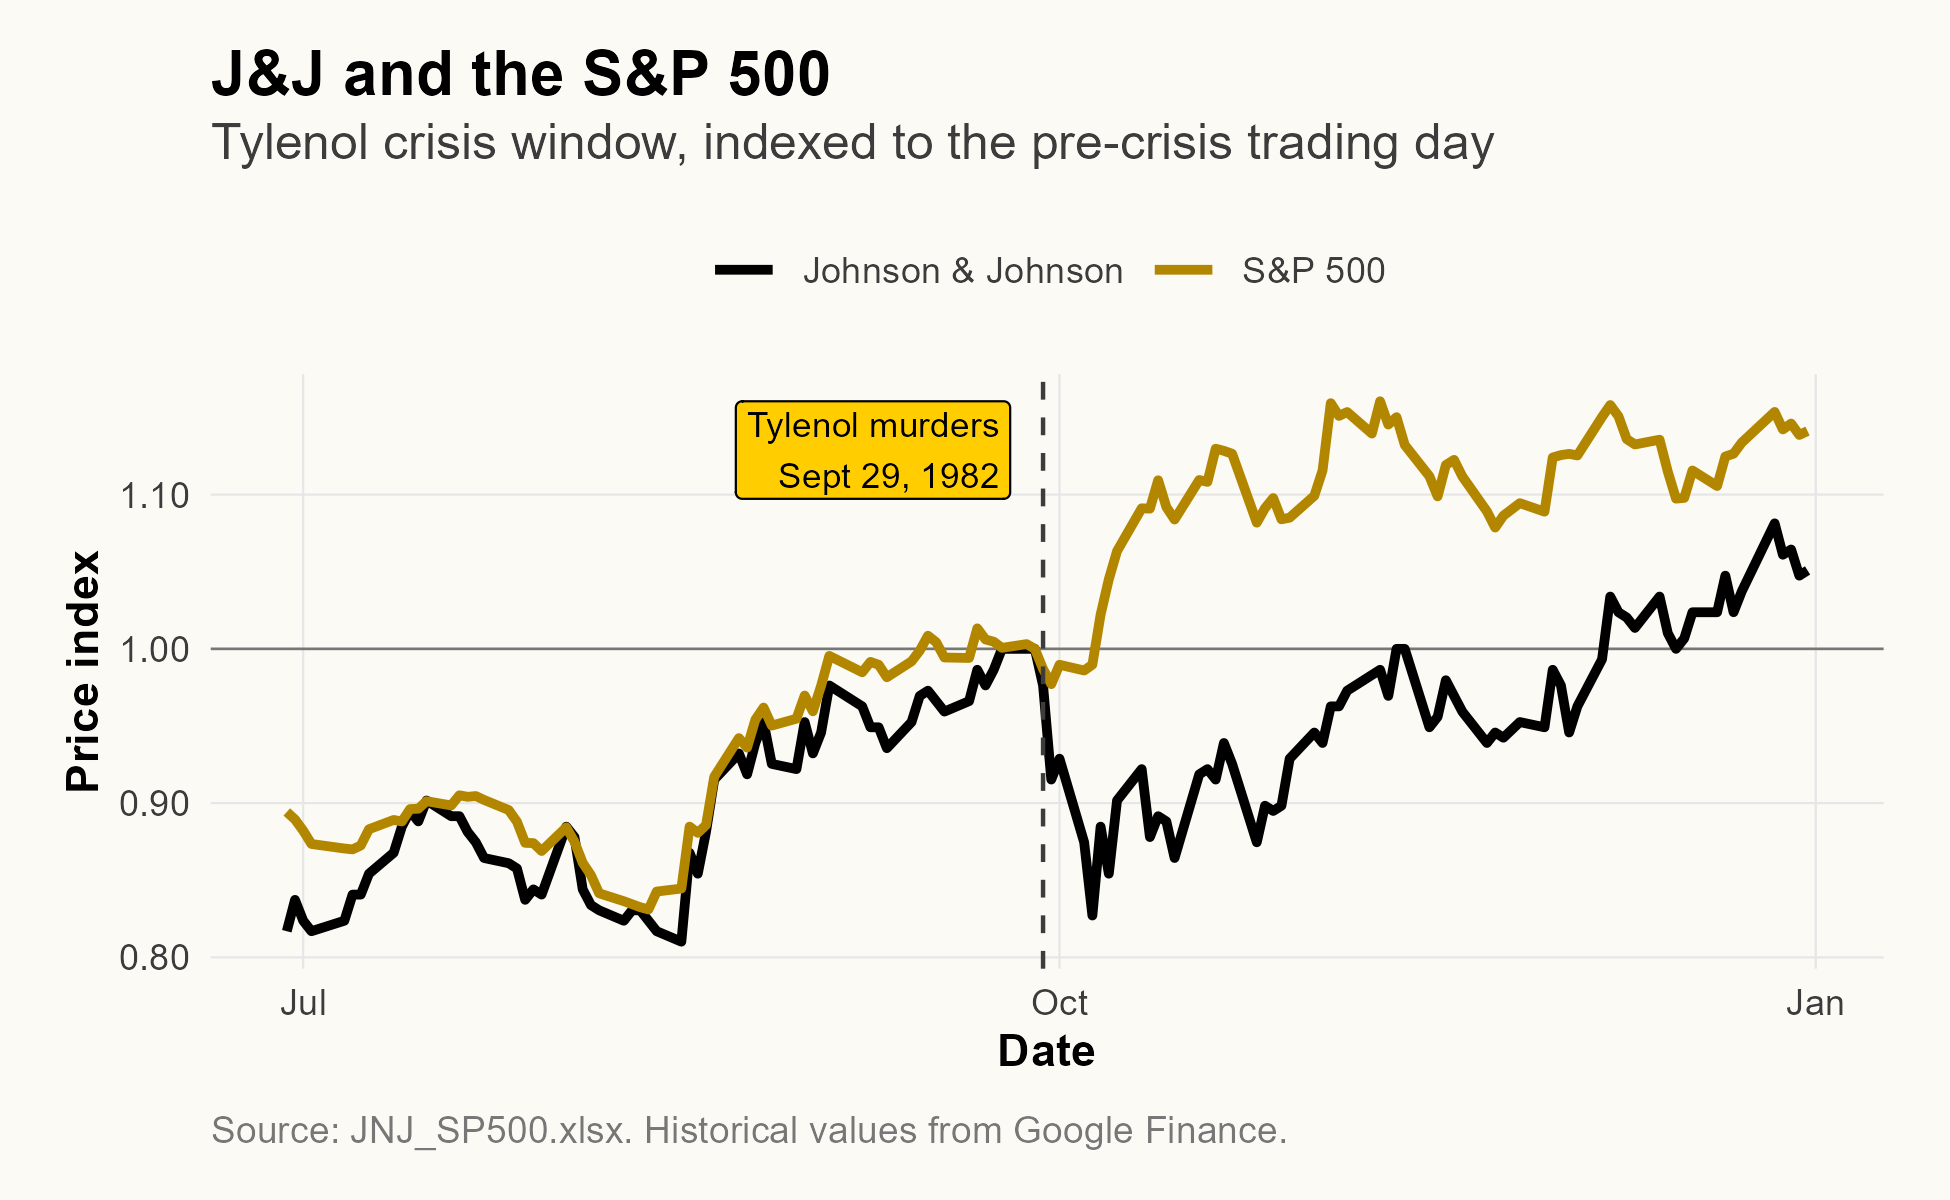
\includegraphics[width=\textwidth]{c1_jnjplot.png}
  \caption{Johnson \& Johnson's stock price fell sharply after the Tylenol murders, but the recovery by late 1982 suggests that the recall, communication strategy, and packaging redesign helped restore investor confidence.}
  \label{fig:jnj-tylenol}
  \figurenote{Both series are indexed to the last available trading day before September 29, 1982.}
\end{figure}

\section{Introduction: The Paradox of Risk Management}\label{introduction-the-paradox-of-risk-management}

Corporate risk management is a large and growing business. Firms purchase billions of dollars of insurance annually, employ sophisticated hedging strategies using derivatives, hire Chief Risk Officers\index{Chief Risk Officer (CRO)}, and establish elaborate risk management committees\index{risk committee} at the board level. Yet modern finance theory, rooted in the seminal work of Modigliani and Miller and the Capital Asset Pricing Model, suggests that under certain idealized conditions, these activities should be irrelevant to firm value. If capital markets are frictionless and investors can costlessly diversify away firm-specific risks, why should a corporation expend resources managing risks that shareholders can eliminate on their own?

This is the \emph{paradox of risk management}\index{risk management!paradox of}. In theory, risk management should not matter; in practice, it clearly does. Resolving this paradox is central to understanding enterprise risk management (ERM)\index{enterprise risk management (ERM)} and its role in corporate strategy.

The answer lies in recognizing that the assumptions underlying the irrelevance propositions---perfect capital markets, no taxes, no bankruptcy costs, symmetric information, and so on---do not hold in the real world. Each departure from these assumptions represents a \emph{friction}\index{market frictions} that can make risk management value-creating. Corporate risk management matters precisely because the idealized world of MM and CAPM does not exist. By reducing the impact of these frictions, risk management can increase firm value, lower the cost of capital, preserve financial flexibility, and improve decision-making.

This chapter proceeds in two parts. First, we carefully lay out the benchmark case: the assumptions and logic that lead to the irrelevance of risk management. Understanding this benchmark is essential; it tells us \emph{when} and \emph{why} risk management should not add value, and it provides a clear framework for identifying when it can. Second, we systematically examine the real-world frictions that break irrelevance and explain how risk management addresses each one. We conclude by introducing the \emph{cost of risk}\index{cost of risk}---a unifying concept that captures the total economic burden of uncertainty---and positioning the objective of corporate risk management as minimizing this cost subject to strategic goals.


\section{The Benchmark: Risk Management Is Irrelevant in Perfect Markets}\label{the-benchmark-risk-management-is-irrelevant-in-perfect-markets}

\subsection{The Modigliani--Miller Propositions}\label{the-modiglianimiller-propositions}

The Modigliani--Miller (MM) theorems\index{Modigliani-Miller propositions} are among the most influential results in corporate finance. In their 1958 paper, Modigliani and Miller demonstrated that, under a set of idealized assumptions, the value of a firm is independent of its capital structure. Whether a firm finances itself with debt or equity does not affect the total value available to all security holders. This result is sometimes called \emph{capital structure irrelevance}\index{capital structure irrelevance}.

The intuition is straightforward. In a perfect market, investors can replicate any capital structure on their own by borrowing or lending at the risk-free rate. If a firm is ``too conservative'' and holds little debt, an investor who prefers leverage can borrow personally to increase exposure. Conversely, if a firm is highly levered, an investor seeking less risk can lend at the risk-free rate to offset the firm's leverage. Because investors can costlessly undo the firm's financing decisions, those decisions do not affect firm value. The value of the firm is determined solely by its real assets and investment opportunities, not by how those assets are financed.

In subsequent work, Modigliani and Miller extended their analysis to dividend policy, again concluding irrelevance under the same frictionless assumptions. The logic generalizes to other corporate financial decisions, including risk management. If hedging, insurance, or other risk management activities merely rearrange cash flows without changing their expected present value, and if investors can replicate or undo these arrangements at zero cost, then risk management is irrelevant to firm value.

\subsection{The Capital Asset Pricing Model (CAPM)}\label{the-capital-asset-pricing-model-capm}

The Capital Asset Pricing Model\index{Capital Asset Pricing Model (CAPM)}, developed independently by Sharpe, Lintner, and others in the mid-1960s, provides a complementary perspective. CAPM describes the relationship between risk and expected return in equilibrium. According to CAPM, the expected return on any risky asset \emph{i} is:

\[
E[R_i] = R_f + \beta_i \left( E[R_M] - R_f \right)
\]

where:

\begin{itemize}
\tightlist
\item
  \(E[R_i]\) is the expected return on asset \emph{i},
\item
  \(R_f\) is the risk-free rate,
\item
  \(\beta_i\) measures the asset's sensitivity to the market portfolio,
\item
  \(E[R_M]\) is the expected return on the market portfolio.
\end{itemize}

The key insight of CAPM is that only \emph{systematic risk}\index{systematic risk}---risk that cannot be diversified away---is priced in equilibrium. Systematic risk, captured by beta\index{beta}, reflects the asset's covariance with the overall market. \emph{Idiosyncratic} or \emph{firm-specific} risk\index{idiosyncratic risk}, by contrast, can be eliminated by holding a diversified portfolio\index{diversification}. Because investors are assumed to hold well-diversified portfolios, they do not require compensation for bearing idiosyncratic risk.

For corporate risk management, the implication is stark: activities that reduce only firm-specific risk---such as insuring against fire, hedging commodity price exposure specific to one firm, or implementing loss control measures against operational hazards---do not reduce systematic risk and therefore do not lower the firm's cost of capital or increase its value. Investors can achieve the same risk reduction by diversifying their portfolios across many firms.

\subsection{Risk Management Irrelevance Under Perfect Markets}\label{risk-management-irrelevance-under-perfect-markets}

Combining the MM and CAPM logic, we arrive at the \emph{irrelevance of corporate risk management}\index{risk management!irrelevance of} under idealized conditions. If:

\begin{itemize}
\tightlist
\item
  Capital markets are perfect and frictionless,\index{perfect markets}
\item
  Investors can diversify away firm-specific risk costlessly,
\item
  There are no taxes, bankruptcy costs, or other distortions,
\end{itemize}

then corporate risk management decisions---hedging\index{hedging}, insurance, loss control spending---do not change firm value. Shareholders can replicate any risk profile they desire by adjusting their own portfolios. A firm that hedges its currency exposure, for example, merely substitutes stable cash flows for volatile ones without changing the expected present value of those cash flows. An investor who prefers the original, unhedged volatility can take offsetting positions in currency markets. Because risk management is redundant, it is irrelevant.

This benchmark does not mean risk management is useless or irrational. Rather, it establishes the conditions under which risk management would \emph{not} add value. It tells us that the rationale for corporate risk management must lie in violations of the perfect-market assumptions. Each friction or imperfection is a potential source of value creation through risk management.


\section{Assumptions Behind CAPM and MM Irrelevance}\label{assumptions-behind-capm-and-mm-irrelevance}

To understand when and why risk management matters, we must clearly articulate the assumptions underlying the irrelevance propositions. These assumptions define the idealized world in which risk management is redundant. In the following subsections, we list and explain these assumptions in detail.

\subsection{Detailed CAPM Assumptions}\label{detailed-capm-assumptions}

The Capital Asset Pricing Model rests on a set of strong assumptions\index{perfect markets!assumptions} about investor behavior and market structure. These assumptions are deliberately simplified to yield tractable predictions; they are not meant to be realistic descriptions of actual markets. Understanding them helps us identify where real-world departures create opportunities for value-adding risk management.

\textbf{Assumption 1: Frictionless Markets}

Markets are assumed to operate without transaction costs\index{transaction costs}, bid--ask spreads, or taxes. Investors can buy and sell any security instantly and costlessly. Securities are perfectly divisible, so investors can hold any fractional amount. There are no regulatory constraints, trading limits, or short-sale restrictions.

In such a world, adjusting one's portfolio is trivial. An investor can instantaneously and costlessly replicate or undo any risk management action a firm takes. This frictionless trading is essential to the irrelevance result: if trading were costly, investors might prefer firms to manage certain risks on their behalf.

\textbf{Assumption 2: Homogeneous Expectations}

All investors share identical beliefs about the expected returns, variances, and covariances of all assets. There is no disagreement about the probability distribution of future outcomes. Everyone uses the same information set and interprets it identically.

Homogeneous expectations ensure that all investors face the same investment opportunity set and agree on the efficient frontier. Without this assumption, different investors might value the same asset differently, and corporate risk management could serve to resolve or exploit these differences.

\textbf{Assumption 3: Single-Period Horizon}

All investors plan over a single, common time horizon. They care only about the distribution of wealth at the end of that period. There are no intermediate consumption needs, no differences in investment horizons, and no multi-period dynamic considerations.

This assumption simplifies the analysis by eliminating intertemporal concerns. In reality, firms and investors face multiple periods, varying liquidity needs, and evolving risks, which can make risk management valuable for managing cash flow timing and ensuring continuous access to capital.

\textbf{Assumption 4: Mean--Variance Preferences}

Investors care only about the mean and variance of portfolio returns.\index{mean-variance preferences} Higher expected return is desirable; higher variance is undesirable. Risk aversion is captured entirely by preferences over these two moments.

This assumption implies that investors are indifferent to higher moments (skewness, kurtosis) and that all risk is adequately summarized by variance. In practice, investors may care about downside risk, extreme events, and the shape of return distributions---concerns that motivate risk management tools like insurance and tail-risk hedging.

\textbf{Assumption 5: Risk-Free Asset and Unlimited Borrowing/Lending}

There exists a risk-free asset offering a known, certain return. All investors can borrow or lend unlimited amounts at this risk-free rate without constraints or credit limits.

In reality, borrowing rates typically exceed lending rates, and borrowing capacity is limited, especially during crises. Firms and investors face collateral constraints and varying access to credit. These imperfections can make internal cash flow stability---enhanced by risk management---valuable for maintaining investment.

\textbf{Assumption 6: All Assets Are Tradable and Marketable}

Every source of risk can be bought, sold, and held in a diversified portfolio. There are no non-traded risks such as private human capital, reputation, or firm-specific knowledge.

In practice, many important risks are not tradable. Managers' human capital is firm-specific and cannot be diversified. Reputation and customer relationships are intangible and illiquid. These non-traded risks can make managers more risk-averse than diversified shareholders, creating a role for corporate risk management to align interests.

\textbf{Assumption 7: Perfect and Symmetric Information}

All information relevant to asset valuation is costlessly and instantly available to all investors. There is no information asymmetry between managers and shareholders, or among investors. Everyone observes the same signals and interprets them identically.

In reality, managers typically know more about their firm's risks and prospects than outside investors do. This information asymmetry can lead to adverse selection and moral hazard\index{moral hazard} problems. Risk management and disclosure policies can mitigate these problems, improving firm value.

\textbf{Assumption 8: No Bankruptcy or Financial Distress Costs}

Default and financial distress are costless events. Bankruptcy is simply a transfer of ownership from equity holders to debt holders, with no loss of value in the process. There are no legal fees, no lost customers, no disrupted operations.

In practice, bankruptcy and financial distress impose substantial direct costs (legal and administrative expenses) and indirect costs (lost customers, suppliers demanding stricter terms, key employees departing). Risk management that reduces the probability of distress can therefore add value.

\textbf{Assumption 9: No Taxes or Neutral Tax Treatment}

There are no corporate or personal taxes, or taxes are neutral and symmetric (gains and losses treated identically, no progressivity, unlimited loss carryforwards and carrybacks at full value).

Real tax systems are not neutral. Corporate tax rates may be progressive, loss offsets are limited, and tax timing matters. Volatile income can increase expected taxes due to convexity and loss limitations. Risk management that smooths taxable income can reduce expected tax liabilities.

\textbf{Assumption 10: No Agency Costs or Conflicts of Interest}

Managers act perfectly in the interests of shareholders. There are no conflicts between managers and owners, or between different classes of security holders. Compensation contracts align incentives perfectly.

In reality, managers have their own objectives, which may not fully align with shareholder value maximization. Risk management and governance mechanisms help mitigate these agency problems and can increase firm value.

\subsection{Modigliani--Miller Assumptions (Overlapping with CAPM)}\label{modiglianimiller-assumptions-overlapping-with-capm}

The MM irrelevance propositions rely on similar assumptions:

\begin{enumerate}
\def\labelenumi{\arabic{enumi}.}
\tightlist
\item
  \textbf{No taxes} (or neutral, symmetric tax treatment).
\item
  \textbf{No transaction or issuance costs} for securities.
\item
  \textbf{Symmetric information} between managers and investors.
\item
  \textbf{No bankruptcy or financial distress costs.}
\item
  \textbf{Firms and individuals can borrow and lend at the same rates} (perfect capital markets).
\item
  \textbf{Investment policy is fixed and independent of financing decisions} (no underinvestment or overinvestment problems).
\end{enumerate}

The overlap between CAPM and MM assumptions is substantial. Both models rely on frictionless markets, perfect information, no taxes, and no distress costs. The irrelevance of risk management follows naturally: if shareholders can costlessly replicate or undo the firm's risk management actions, those actions do not affect firm value. The firm's value depends only on its real investment opportunities and the systematic risk of its cash flows.

\subsection{What Irrelevance Means}\label{what-irrelevance-means}

Understanding irrelevance is crucial. Irrelevance does \emph{not} mean that risk or risk management is unimportant in some absolute sense. Rather, it means that, under the stated assumptions, corporate risk management decisions do not affect firm value because they are redundant. Anything the firm does to manage risk can be undone or replicated by shareholders in their own portfolios at zero cost.

For example:

\begin{itemize}
\tightlist
\item
  If a firm hedges interest rate exposure, a shareholder who wants that exposure can take an offsetting position in interest rate derivatives.
\item
  If a firm buys fire insurance, a diversified shareholder already holds a portfolio that averages away the idiosyncratic fire risk across many firms.
\item
  If a firm smooths earnings through hedging, investors can ``see through'' the smoothing and value the firm based on its underlying cash flows.
\end{itemize}

Irrelevance is a powerful benchmark because it isolates the question: \emph{What conditions must fail for risk management to add value?} The answer is that real-world frictions---taxes, distress costs, agency problems, information asymmetries, regulatory constraints, and investment inflexibilities---break irrelevance and create opportunities for value-enhancing risk management.


\section{Real-World Frictions That Make Risk Management Matter}\label{real-world-frictions-that-make-risk-management-matter}

The value of corporate risk management arises from violations of the perfect-market assumptions. Each friction represents a wedge between the idealized benchmark and actual corporate finance. In this section, we examine the major frictions and explain how risk management can mitigate their costs, thereby increasing firm value.

\subsection{Taxes and Tax Convexity}\label{taxes-and-tax-convexity}

\textbf{The Friction: Progressive and Convex Tax Schedules}

Real corporate tax systems are not neutral.\index{taxes!and risk management} Tax rates may be progressive, rising with income. Losses and gains are not treated symmetrically: losses can often be carried forward or back, but with limitations. Net operating loss carryforwards\index{net operating loss carryforwards} may expire, and their present value is reduced by discounting and uncertainty. In some jurisdictions, the tax code includes exemptions, deductions, and credits that phase in or out, creating convexity in the effective tax schedule\index{tax convexity}.

\textbf{How Volatility Increases Expected Taxes}

When the tax function is convex, Jensen's inequality\index{Jensen's inequality} implies that the expected tax liability on a volatile stream of income exceeds the tax liability on a stable stream with the same expected value. Intuitively, in high-income years the firm pays tax at a high marginal rate, while in low-income (or loss) years, the tax benefit of losses is limited or delayed. Averaging over many periods, the volatile firm pays more in expected present-value taxes than a stable firm with identical expected income.

\textbf{Simple Example}

Consider a firm facing a progressive tax schedule:

\begin{itemize}
\tightlist
\item
  Income below \$100 million: 20\% tax rate.
\item
  Income above \$100 million: 30\% tax rate.
\end{itemize}

Firm A (stable): Earns \$100 million each year. Tax: \$20 million per year.

Firm B (volatile): Earns \$50 million in bad years, \$150 million in good years (average \$100 million). In bad years: tax = \$10 million. In good years: tax on first \$100 million = \$20 million, tax on next \$50 million = \$15 million, total = \$35 million. Average tax = \(\frac{10 + 35}{2} = \$22.5\) million.

Firm B pays \$2.5 million more in expected taxes annually solely because of volatility, even though expected pre-tax income is the same.

\textbf{How Risk Management Adds Value}

By using hedging, insurance, or other tools to smooth taxable income, risk management reduces the expected present value of taxes. Reducing income volatility shifts the firm toward the stable case, lowering the average tax rate. The tax savings increase after-tax cash flows and firm value.

This friction is one of the most straightforward and empirically supported rationales for corporate hedging and risk management.

\subsection{Costly Financial Distress and Bankruptcy}\label{costly-financial-distress-and-bankruptcy}

\textbf{The Friction: Bankruptcy Is Not Costless}

Under the MM assumptions, bankruptcy is merely a transfer of ownership from equity holders to debt holders, with no destruction of value. In reality, bankruptcy and financial distress impose significant costs:\index{financial distress!costs of}\index{bankruptcy costs}

\begin{itemize}
\tightlist
\item
  \textbf{Direct costs}: Legal fees, court costs, advisory fees, and administrative expenses. These costs can consume a substantial fraction of firm value, especially for smaller firms.
\item
  \textbf{Indirect costs}: Before and during bankruptcy, customers may flee (fearing disrupted service or warranty claims), suppliers may demand stricter payment terms or refuse to deal, key employees may depart, and the firm may lose valuable intangible assets like reputation and brand. Investment and innovation often stall. Competitors may poach market share.
\end{itemize}

Studies suggest that direct costs alone can be 3--5\% of firm value, and indirect costs can be much larger, sometimes exceeding 10--20\% of pre-distress value for firms in industries where reputation and customer confidence are critical.

\textbf{How Volatility Increases Distress Costs}

High volatility of cash flows and earnings increases the probability that the firm will face financial distress or default, especially if the firm is leveraged. The expected cost of distress is:

\[
\text{Expected Distress Cost} = \Pr(\text{Distress}) \times \text{Cost if Distressed}
\]

By increasing \(\Pr(\text{Distress})\), volatility raises the expected distress cost, reducing firm value.

\textbf{How Risk Management Adds Value}

Risk management reduces cash flow volatility, which in turn reduces the probability of distress. For example:

\begin{itemize}
\tightlist
\item
  Hedging commodity price or currency risks stabilizes operating cash flows.
\item
  Purchasing insurance\index{insurance} against property damage, liability, or business interruption\index{business interruption} ensures that large, unexpected losses do not push the firm into distress.
\item
  Managing liquidity through credit lines or cash reserves provides a buffer against shocks.
\end{itemize}

By lowering the expected present value of distress costs, risk management increases firm value. This benefit is particularly large for highly leveraged firms or firms in industries with high indirect distress costs.

\subsection{Investment Distortions and Underinvestment}\label{investment-distortions-and-underinvestment}

\textbf{The Friction: Financial Constraints and Limited Access to External Capital}

The MM framework assumes that firms can always finance positive-NPV projects by issuing securities at fair prices. In reality, external finance is costly and often limited, especially during downturns or after negative shocks. Asymmetric information and agency problems raise the cost of external capital. During crises or firm-specific shocks, access to capital markets may dry up entirely, or new equity can be issued only at a steep discount.

\textbf{The Underinvestment Problem}

When a firm faces a valuable investment opportunity but lacks internal funds and cannot raise external capital at reasonable terms, it may forgo the project. This is the \emph{underinvestment problem}\index{underinvestment problem}, famously analyzed in the context of debt overhang\index{debt overhang} and financial constraints. Missing positive-NPV projects reduces firm value.

Volatile cash flows exacerbate underinvestment. If the firm's cash flows are highly uncertain, it is more likely to find itself short of funds precisely when investment opportunities arise. Without hedging or insurance, internal funds may be depleted by unrelated shocks (e.g., commodity price swings, currency losses, catastrophic property damage), forcing the firm to pass on valuable projects.

\textbf{How Risk Management Adds Value}

Risk management smooths and stabilizes internal cash flows. By doing so, it ensures that the firm has predictable funds available to seize investment opportunities as they arise. This is sometimes described as \emph{preserving financial flexibility}\index{financial flexibility} or \emph{protecting the option to invest}.

\textbf{Simple Example}

Consider a firm with a valuable growth project requiring \$50 million. The firm's internal cash flow is either \$30 million (bad state) or \$70 million (good state), each with 50\% probability. External finance is costly or unavailable.

\begin{itemize}
\tightlist
\item
  \textbf{Without hedging}: In the bad state, the firm cannot fund the project (shortfall of \$20 million). The firm loses the NPV of the project in that state. Expected loss = 50\% of project NPV.
\item
  \textbf{With hedging}: The firm smooths cash flow to \$50 million in each state (paying in good states, receiving in bad states). Now the firm can fund the project in \emph{all} states. Expected loss = 0.
\end{itemize}

By enabling consistent investment, risk management captures the full expected NPV of the project, increasing firm value.

This rationale is empirically important. Studies find that firms with greater cash flow volatility invest less, and that hedging is positively associated with investment, especially for financially constrained firms.

\subsection{Principal--Agent Problems and Managerial Incentives}\label{principalagent-problems-and-managerial-incentives}

\textbf{The Friction: Misaligned Incentives Between Managers and Shareholders}

MM and CAPM assume that managers act perfectly in shareholders' interests. In reality, managers are agents of shareholders (the principals), and their incentives are not perfectly aligned. This creates \emph{agency costs}\index{agency costs}\index{principal-agent problem}.

Managers face firm-specific risks that they cannot diversify away:

\begin{itemize}
\tightlist
\item
  Their human capital\index{human capital!managerial} is tied to the firm. If the firm performs poorly or fails, the manager loses income, reputation, and future career prospects.
\item
  Managerial compensation is often closely tied to firm performance (salary, bonus, equity grants).
\end{itemize}

As a result, managers may be more risk-averse than well-diversified shareholders, leading them to avoid risky (but positive-NPV) projects or to over-invest in hedging and insurance beyond what shareholders would prefer.

Conversely, under some compensation structures (e.g., heavy reliance on stock options), managers may become \emph{too} risk-loving, taking excessive risks to increase the option value of their compensation (``gambling for resurrection'')\index{gambling for resurrection}.

\textbf{How Risk Management Can Align Incentives}

Well-designed risk management and governance can help align managerial risk-taking with shareholder preferences:

\begin{enumerate}
\def\labelenumi{\arabic{enumi}.}
\item
  \textbf{Reducing uncompensated managerial risk aversion}: By hedging or insuring risks that are unrelated to the firm's core strategy (e.g., commodity price risk for a non-commodity firm), risk management reduces volatility that worries managers but does not concern diversified shareholders. This frees managers to take value-creating strategic risks.
\item
  \textbf{Constraining excessive risk-taking}: Board-level risk limits, hedging policies, and enterprise-wide risk frameworks can prevent managers from ``gambling'' with firm assets when compensation incentives are misaligned. Risk committees and independent oversight complement compensation design.
\item
  \textbf{Improving performance measurement and incentive contracting}: By smoothing noise and clarifying performance, risk management makes it easier to design effective incentive contracts. Cleaner signals of managerial effort and skill improve the efficiency of compensation.
\end{enumerate}

\textbf{Example}

A CEO whose wealth is heavily invested in company stock may be reluctant to undertake a risky (but high-NPV) international expansion because failure could devastate her personal wealth. If the firm hedges exchange rate and political risks associated with the expansion, the CEO's personal risk is reduced, and she is more willing to pursue the value-creating project. The hedging realigns her incentives with those of diversified shareholders.

\subsection{Information Asymmetry and Signaling}\label{information-asymmetry-and-signaling}

\textbf{The Friction: Managers Know More Than Investors}

Perfect markets assume symmetric information. In reality, managers possess private information about the firm's risks, opportunities, and prospects. This \emph{information asymmetry}\index{information asymmetry} creates several problems:

\begin{itemize}
\tightlist
\item
  \textbf{Adverse selection}\index{adverse selection}: Investors cannot perfectly distinguish high-quality firms from low-quality ones. They demand a risk premium to compensate for uncertainty, raising the firm's cost of capital.
\item
  \textbf{Undervaluation}: Good firms may be systematically undervalued if investors cannot observe quality. This can lead to underinvestment in equity or foregone opportunities.
\item
  \textbf{Earnings opacity}: Volatile, hard-to-interpret earnings make it difficult for investors to assess managerial performance and firm fundamentals, again increasing required returns.
\end{itemize}

\textbf{How Risk Management Reduces Information Asymmetry}

Risk management can improve the transparency and credibility of the firm's reported performance:

\begin{enumerate}
\def\labelenumi{\arabic{enumi}.}
\item
  \textbf{Smoothing idiosyncratic noise}: Hedging and insurance reduce volatility from sources unrelated to managerial actions or strategic choices. This makes it easier for investors to identify the firm's core performance and prospects. For example, hedging currency risk allows investors to evaluate operating performance without the noise of exchange rate fluctuations.
\item
  \textbf{Signaling quality}\index{signaling}: A firm's willingness to commit to risk management policies can serve as a credible signal. For example, a firm that hedges consistently may signal confidence in its core business and a long-term orientation, differentiating itself from opportunistic or lower-quality competitors.
\item
  \textbf{Reducing cost of capital}\index{cost of capital}: Lower information asymmetry reduces the adverse selection premium investors demand, lowering the firm's cost of equity and debt.
\end{enumerate}

\textbf{Example}

Consider two firms with identical expected operating income but different hedging policies. Firm A hedges its commodity exposure; Firm B does not. Firm B's reported earnings are volatile, partly due to commodity price swings. Investors cannot easily separate operational performance from commodity luck. They demand a higher return to compensate for this uncertainty. Firm A's hedged earnings are more stable and informative, reducing the information premium and lowering the cost of capital.

\subsection{Contracting and Stakeholder Relationships}\label{contracting-and-stakeholder-relationships}

\textbf{The Friction: Long-Term Relationships Are Sensitive to Firm Risk}

Firms operate within a web of relationships: employees, customers, suppliers, distributors, regulators, and communities.\index{stakeholder relationships} Many of these relationships involve explicit or implicit long-term contracts\index{implicit contracts}. For example:

\begin{itemize}
\tightlist
\item
  Employees expect stable employment and career development.
\item
  Customers rely on warranties, service, and product quality.
\item
  Suppliers invest in relationship-specific assets.
\item
  Distributors commit resources to promote the firm's products.
\end{itemize}

These relationships are vulnerable to firm distress. If a firm experiences a severe negative shock, it may:

\begin{itemize}
\tightlist
\item
  Lay off workers, breaking implicit employment commitments.
\item
  Cut quality or service, damaging customer trust.
\item
  Default on supplier payments, disrupting the supply chain.
\item
  Lose regulatory licenses or face stricter oversight.
\end{itemize}

\textbf{How Volatility Damages Relationships}

High volatility increases the risk of extreme negative outcomes that jeopardize relationships. Stakeholders---who are not diversified with respect to this specific firm---will demand compensation for bearing this risk or will reduce their commitment. For example:

\begin{itemize}
\tightlist
\item
  Employees may demand higher wages to compensate for job insecurity, or top talent may leave for more stable firms.
\item
  Customers may avoid products from a financially unstable firm (especially for durable goods or products requiring after-sale support).
\item
  Suppliers may demand cash-in-advance or refuse credit.
\item
  Lenders and bondholders will demand higher interest rates.
\end{itemize}

\textbf{How Risk Management Protects Relationships}

By reducing the probability of extreme adverse outcomes, risk management helps the firm honor implicit and explicit commitments:

\begin{itemize}
\tightlist
\item
  Insurance and hedging make it more likely the firm can maintain employment during downturns.
\item
  Product liability insurance and quality controls credibly commit the firm to stand behind its products, enhancing brand and sales.
\item
  Financial stability allows the firm to negotiate better terms with suppliers and distributors.
\end{itemize}

The result is lower contracting costs and more valuable long-term relationships, increasing firm value.

\subsection{Regulatory and Rating-Agency Constraints}\label{regulatory-and-rating-agency-constraints}

\textbf{The Friction: Capital Requirements, Regulation, and Credit Ratings}

Many industries are subject to regulatory oversight that ties capital requirements or operating permissions to measures of financial stability:

\begin{itemize}
\tightlist
\item
  \textbf{Banks and insurers} face risk-based capital requirements\index{capital requirements!regulatory}. Volatile earnings and capital ratios can trigger regulatory intervention or require costly capital raises.
\item
  \textbf{Utilities} are regulated and their rate-setting depends on perceived risk and cost of capital.
\item
  \textbf{Credit ratings}\index{credit ratings}: Rating agencies\index{rating agencies} penalize earnings volatility and reward consistent risk management. Higher ratings reduce borrowing costs and improve access to capital markets.
\end{itemize}

\textbf{How Risk Management Adds Value Under Regulation}

Risk management that reduces volatility and smooths capital ratios helps firms:

\begin{itemize}
\tightlist
\item
  Maintain or improve credit ratings, lowering the cost of debt and expanding the investor base.
\item
  Avoid breaching regulatory capital thresholds, which can trigger expensive corrective actions or restrict business growth.
\item
  Demonstrate prudent governance to regulators, reducing the risk of additional regulation or penalties.
\end{itemize}

\textbf{Example}

An insurance company that uses reinsurance\index{reinsurance} and hedging to reduce underwriting volatility will have more stable surplus levels. This stability supports a higher credit rating, which in turn allows the company to write more business at better terms and reduces its cost of debt. The value created by improved ratings and regulatory standing justifies the cost of reinsurance and hedging.


\section{The Cost of Risk and the Objective of Corporate Risk Management}\label{the-cost-of-risk-and-the-objective-of-corporate-risk-management}

\subsection{Defining the Cost of Risk}\label{defining-the-cost-of-risk}

After examining the frictions individually, it is useful to introduce a unifying framework: the \emph{cost of risk}\index{cost of risk!components}. The cost of risk is the total economic burden a firm bears because its future outcomes are uncertain. It includes both direct costs (such as insurance premiums and retained losses) and indirect costs (the value destroyed by volatility through taxes, distress, agency, information, and regulatory channels).

We can express the cost of risk schematically as:

\[
\begin{aligned}
\text{Cost of Risk} ={}& \text{Expected Retained Losses} + \text{Risk Control Costs} \\
&+ \text{Risk Financing Costs} + \text{Indirect Costs of Volatility}
\end{aligned}
\]

\textbf{Components:}

\begin{enumerate}
\def\labelenumi{\arabic{enumi}.}
\item
  \textbf{Expected Retained Losses}\index{retained losses}: The present value of losses the firm will bear directly (deductibles, uninsured losses, etc.).
\item
  \textbf{Risk Control Costs}\index{loss control}: Expenditures on loss prevention, safety programs, quality control, cybersecurity, and other measures to reduce the frequency or severity of losses.
\item
  \textbf{Risk Financing Costs}\index{risk financing}: Premiums for insurance, fees for hedging instruments, costs of maintaining credit lines, and administrative costs of risk management programs.
\item
  \textbf{Indirect Costs of Volatility}: The deadweight losses arising from frictions:

  \begin{itemize}
  \tightlist
  \item
    Increased expected taxes due to convexity.
  \item
    Expected bankruptcy and distress costs.
  \item
    Underinvestment and foregone positive-NPV projects.
  \item
    Agency costs and misaligned incentives.
  \item
    Information asymmetry and higher cost of capital.
  \item
    Damaged stakeholder relationships.
  \item
    Regulatory penalties or increased capital requirements.
  \end{itemize}
\end{enumerate}

\subsection{The Objective of Corporate Risk Management}\label{the-objective-of-corporate-risk-management}

The goal of corporate risk management is \emph{not} to eliminate all risk. Risk is inseparable from return; eliminating risk would also eliminate profitable opportunities. Rather, the objective is to \textbf{minimize the total cost of risk, subject to the firm's strategic goals and risk appetite}\index{cost of risk!minimization}\index{risk appetite}.

In practice, this means:

\begin{itemize}
\tightlist
\item
  Identifying and measuring the firm's key risks.
\item
  Deciding which risks to retain\index{risk retention} (because the firm has a comparative advantage in bearing them, or because they are integral to the firm's business model), and which to transfer or mitigate\index{risk transfer}.
\item
  Selecting cost-effective tools---insurance, hedging, diversification, loss control---to manage retained risks.
\item
  Balancing the direct costs of risk management (premiums, fees, program expenses) against the reduction in indirect costs (tax savings, lower distress costs, preserved investment, etc.).
\end{itemize}

\textbf{Key Insight}: Risk management is valuable when the reduction in indirect costs exceeds the direct costs of implementing it. A firm should hedge, insure, or otherwise manage a risk if doing so reduces the total cost of risk by more than it costs to execute.

\subsection{Risk Management as Core Corporate Finance}\label{risk-management-as-core-corporate-finance}

Viewed through this lens, risk management is not a separate, specialized function. It is integral to corporate finance and strategy. Every major corporate decision---capital structure, dividend policy, investment, hedging---affects the firm's risk profile and hence the cost of risk.

Effective enterprise risk management:

\begin{itemize}
\tightlist
\item
  Frees up capital and managerial attention by reducing the drag of risk-related frictions.
\item
  Preserves financial flexibility to invest in growth and innovation.
\item
  Aligns incentives and improves governance.
\item
  Enhances transparency and lowers the cost of capital.
\end{itemize}

In short, risk management contributes to the fundamental objective of financial management: \textbf{maximizing firm value}.


\section{Roadmap for the Rest of the Book}\label{roadmap-for-the-rest-of-the-book}

This chapter has established the conceptual foundation for enterprise risk management. We began with the benchmark irrelevance propositions of Modigliani--Miller and the CAPM, which teach us that risk management would not matter in a world of perfect capital markets. We then examined the real-world frictions---taxes, bankruptcy costs, investment constraints, agency problems, information asymmetries, and regulatory pressures---that break irrelevance and create opportunities for value-enhancing risk management. Finally, we introduced the cost of risk as a unifying concept and defined the objective of risk management as minimizing this cost.

The chapters that follow build on this foundation:

\begin{itemize}
\item
  \textbf{Chapter 2: Enterprise Risk Management Frameworks} introduces the organizational and governance structures firms use to implement ERM, including risk committees, risk appetite statements, and the role of the Chief Risk Officer.
\item
  \textbf{Chapter 3: Risk Identification} explores systematic methods for discovering and cataloging the full range of risks a firm faces, from strategic and operational risks to financial and hazard risks.
\item
  \textbf{Chapter 4: Risk Quantification and Qualification} covers techniques for measuring risk, including frequency-severity analysis, loss distributions, Value-at-Risk (VaR), and scenario analysis.
\item
  \textbf{Chapter 5: Risk Appetite and the ERM Process} discusses how firms articulate their willingness to bear risk, set risk limits, and integrate risk considerations into strategic planning.
\item
  \textbf{Chapter 6: Examining the Firm's Risk Portfolio} examines how risks interact, the importance of correlations and diversification within the firm, and how to assess the aggregate risk profile.
\item
  \textbf{Chapter 7: Loss Control and Risk Reduction} analyzes investments in safety, quality, and other measures to reduce the frequency or severity of losses, including cost-benefit analysis.
\item
  \textbf{Chapter 8: Risk Financing and Alternative Risk Transfer} covers insurance, hedging, captives, and other tools for financing retained risk and transferring risk to third parties.
\item
  \textbf{Chapter 9: Corporate Risk Governance} ties together the organizational, board-level, and cultural elements that ensure effective risk management.
\end{itemize}

Throughout the book, we return repeatedly to the theme of this chapter: risk management is valuable when it reduces the cost of risk arising from real-world frictions. By the end, you will have both the conceptual framework and the practical tools to evaluate and improve risk management in any organization.

\begin{center}\rule{0.5\linewidth}{0.5pt}\end{center}

\begin{keytakeaways}
\item
  \textbf{The Irrelevance Benchmark}: Under the idealized assumptions of Modigliani--Miller and the CAPM (frictionless markets, no taxes, no bankruptcy costs, symmetric information, etc.), corporate risk management is irrelevant to firm value. Investors can costlessly replicate or undo any risk management action on their own.
\item
  \textbf{Real-World Frictions Create Value Opportunities}: Risk management becomes valuable when the perfect-market assumptions fail. Key frictions include:

  \begin{itemize}
  \tightlist
  \item
    \textbf{Taxes}: Convex and progressive tax schedules make volatile income more expensive. Smoothing taxable income reduces expected taxes.
  \item
    \textbf{Bankruptcy Costs}: Financial distress imposes direct and indirect costs. Reducing volatility lowers the probability of distress.
  \item
    \textbf{Investment Constraints}: Limited access to external capital can force firms to forgo valuable projects. Risk management preserves internal funds and financial flexibility.
  \item
    \textbf{Agency Problems}: Misaligned incentives between managers and shareholders can lead to suboptimal risk-taking. Risk management and governance help align interests.
  \item
    \textbf{Information Asymmetry}: Private information raises the cost of capital. Risk management reduces noise and signals quality.
  \item
    \textbf{Stakeholder Relationships}: Volatility damages long-term relationships with employees, customers, and suppliers. Stability protects these valuable relationships.
  \item
    \textbf{Regulation and Ratings}: Regulatory capital requirements and credit ratings reward stable performance. Risk management improves standing and lowers costs.
  \end{itemize}
\item
  \textbf{The Cost of Risk}: The total economic burden of uncertainty, comprising expected retained losses, risk control and financing costs, and indirect costs from frictions. The objective of risk management is to minimize this total cost.
\item
  \textbf{Risk Management as Strategy}: Effective risk management is central to corporate finance. It frees resources, preserves flexibility, and ultimately increases firm value by reducing the cost of risk.
\item
  \textbf{Forward Look}: Subsequent chapters provide the frameworks, tools, and governance structures to implement value-creating risk management in practice.
\end{keytakeaways}

\section*{References}
\addcontentsline{toc}{section}{References}
\begingroup
\sloppy

Froot, K. A., Scharfstein, D. S., \& Stein, J. C. (1993). Risk management: Coordinating corporate investment and financing policies. \emph{Journal of Finance}, \emph{48}(5), 1629--1658.

Jensen, M. C., \& Meckling, W. H. (1976). Theory of the firm: Managerial behavior, agency costs and ownership structure. \emph{Journal of Financial Economics}, \emph{3}(4), 305--360.

Lintner, J. (1965). The valuation of risk assets and the selection of risky investments in stock portfolios and capital budgets. \emph{Review of Economics and Statistics}, \emph{47}(1), 13--37.

Modigliani, F., \& Miller, M. H. (1958). The cost of capital, corporation finance and the theory of investment. \emph{American Economic Review}, \emph{48}(3), 261--297.

Myers, S. C. (1977). Determinants of corporate borrowing. \emph{Journal of Financial Economics}, \emph{5}(2), 147--175.

Sharpe, W. F. (1964). Capital asset prices: A theory of market equilibrium under conditions of risk. \emph{Journal of Finance}, \emph{19}(3), 425--442.

Smith, C. W., \& Stulz, R. M. (1985). The determinants of firms' hedging policies. \emph{Journal of Financial and Quantitative Analysis}, \emph{20}(4), 391--405.

\subsection*{Tylenol Case Sources}

Chicago Tylenol murders: 3 members of the Janus family dies in 1982, and pain has passed on to generations. Viewed May 19, 2026. \url{https://www.cbsnews.com/chicago/news/1982-tylenol-poisoning-murders-janus-family/}

Pace, Eric. ``TYLENOL WILL REAPPEAR IN TRIPLE-SEAL PACKAGE.'' November 12, 1982. Viewed May 19, 2026. \url{https://www.nytimes.com/1982/11/12/business/tylenol-will-reappear-in-triple-seal-package.html}

Chicago Tylenol murders. Viewed May 19, 2026. \url{https://grokipedia.com/page/Chicago_Tylenol_murders}

Johnson \& Johnson. Viewed May 19, 2026. \url{https://www.ou.edu/deptcomm/dodjcc/groups/02C2/Johnson\%20\&\%20Johnson.htm}

\endgroup
\end{document}

\input{"../chapter_02/Chapter_02_Enterprise_Risk_Management.tex"}
% !TeX root = Chapter_03_Risk_Identification.tex
% Chapter 3 — Risk Identification: Categorizing and Discovering Enterprise Risks
\documentclass[11pt,openany]{book}
\usepackage{graphicx}
\usepackage{amsmath,amssymb}
\usepackage{hanging}
\makeatletter
\def\input@path{{second_ed/style/}{../style/}}
\makeatother
\usepackage{erm_textbook_style}
\providecommand{\tightlist}{\setlength{\itemsep}{0pt}\setlength{\parskip}{0pt}}
\emergencystretch=2em

\begin{document}

\setcounter{chapter}{2}
\chapter{Risk Identification: Categorizing and Discovering Enterprise Risks}
\label{chap:risk-identification}

\begin{learningobjectives}
  \item Explain why risk identification is the foundational step in enterprise risk management.
  \item Distinguish among hazard, financial, operational, and strategic risks, and identify vivid examples of each.
  \item Explain why financial loss is not the same as financial risk, and classify business interruption correctly.
  \item Describe how risks interact across quadrant boundaries and why siloed identification fails.
  \item Apply internal and external risk identification methodologies to a real organization.
  \item Read and critically evaluate the Risk Factors section of an SEC Form~10-K.
\end{learningobjectives}

\chapteroverview{%
Risk identification is where enterprise risk management begins. Before an organization can assess, prioritize, or respond to risks, it has to see them---and seeing them completely is harder than it sounds. Risks hide in assumptions, emerge gradually from shifts in technology or regulation, and often cross the boundaries of the functions that are supposed to manage them. Chapter~2 established the frameworks and governance structures for ERM. This chapter asks what those structures are supposed to find: what categories of risk exist, where to look for them, and how to tell when you have found something important.

The chapter introduces a four-quadrant taxonomy that organizes risks into hazard, financial, operational, and strategic categories. That structure is a useful organizing device, but its purpose is identification---not administration. The goal of risk identification is not to produce four separate lists managed by four separate functions. It is to build a single, integrated picture of how the organization's risks interact. A supply chain disruption is an operational risk; if it persists, it becomes a strategic risk as customers defect; it may trigger a business interruption insurance claim that is a hazard risk dimension; and if disrupted inputs are commodity-priced, it has a financial dimension too. No one department owns all of that, and no single-category risk register captures it. Understanding the taxonomy is the precondition for seeing across it.

This chapter also addresses the practical challenge of discovering risks. Internal sources---historical losses, audit findings, performance metrics, employee input---provide one lens. External sources---peer disclosures, regulatory guidance, industry data---provide another. For public companies in the United States, the Risk Factors section of the SEC Form~10-K annual report is one of the richest public datasets of structured risk identification available, and we spend considerable time on how to read and use it.%
}

\clearpage

\begin{corporateexample}[Netflix and the Red Envelope Problem]
It started with a red envelope.
\medskip

In the early 2000s, millions of Americans got used to seeing slim red mailers from Netflix\index{Netflix} in their mailboxes. Customers went online, picked a few DVDs, and within days the discs arrived. When they were done, they slipped the discs back into the same envelopes and sent them through the U.S.\ mail. No late fees. No wandering the aisles of a video store on Friday night. For a while, it looked like the future.
\medskip
For Netflix, the DVD-by-mail business was not a side project. It was the business. By the mid-2000s, the company had millions of subscribers, growing revenues, and a clear foil in Blockbuster\index{Blockbuster}, whose brick-and-mortar rental stores suddenly seemed slow and expensive. The logistics system for buying, sorting, and shipping discs was a sophisticated operation. Wall Street liked the story. The red envelope had become a small cultural icon.

\medskip
Inside the company, however, some people were already worrying about what came next.

As early as the mid-2000s, Netflix executives and engineers were tracking a trend that had nothing to do with postal routes: the steady spread of high-speed internet connections into American homes and the rapid improvement of video compression technology. If movies and television could be delivered instantly over the internet, what would that do to a business built around putting plastic discs in the mail? The risk was strategic and operational, not just technical. If Netflix clung to DVDs too long, a rival with better streaming infrastructure could leapfrog it. If it moved too quickly, it could undermine the DVD cash flow that was funding its growth. The company faced a classic problem of disruption\index{technological disruption}: how do you intentionally erode the business model that currently pays your bills, in order to build the one that might keep you alive?

\medskip
Netflix did something that many firms struggle to do. It named this as a concrete, enterprise-level risk. In board discussions, strategic planning, and eventually in the Risk Factors section of its Form~10-K\index{Form 10-K Risk Factors}, management identified a cluster of related uncertainties: that broadband might not spread as fast as expected; that studios might restrict or overprice digital rights; that competitors with ``greater financial, marketing, and technical resources'' could outcompete Netflix in streaming; and that the shift from physical to digital distribution could alienate customers. These were not explanations written after the fact. They were forward-looking statements of risk, made while the DVD business still looked strong.

Acting on that risk identification meant spending money before the payoff was certain. Netflix began hiring engineers to build a streaming platform, negotiating licenses for online content, and experimenting with an early ``Watch Instantly'' feature---all while the red envelopes remained central to revenue. In its public filings, Netflix warned investors that the DVD business could decline faster than expected and that its future depended on successfully managing the transition. In effect, it told shareholders: the engine that powers our current earnings is at risk, and we are deliberately trying to replace it.

\medskip
The transition was messy. In 2011, Netflix tried to split its DVD and streaming services into separate brands. Customers rebelled at the price changes and confusion; the stock price plunged. But the underlying risk assessment---that physical discs were a shrinking technology and that streaming would define the market---did not change. A decade after those first experiments, the red envelopes were disappearing. Blockbuster's stores were gone. Netflix, the former mail-order DVD company, had become a global streaming platform and media producer.
\medskip
From an enterprise risk management perspective, this story is not just about innovation. It is about \textbf{identification}\index{risk identification}. Netflix recognized, early and explicitly, that its own successful business model contained a built-in obsolescence risk. It treated that recognition as a strategic risk, wrote it down in its risk disclosures, and used it to justify reallocating capital before the old model had obviously failed. The most important risks do not always arrive as sudden crises. Some arrive as slow-moving shifts in technology and behavior that turn yesterday's strengths into tomorrow's vulnerabilities---and the hardest part of managing them is simply seeing them in time.

\smallskip
\textit{Source: Netflix, Inc., Annual Report on Form~10-K for the fiscal year ended December~31, 2007, Item~1A ``Risk Factors,'' U.S.\ Securities and Exchange Commission.}
\end{corporateexample}

%--------------------------------------------------------------------
\section{The Four Quadrants of Risk}
\label{sec:four-quadrants}

Risk taxonomies help organizations ensure comprehensive identification and assign appropriate management responsibilities. The framework used in this book organizes risks into four quadrants\index{four-quadrant risk taxonomy}\index{risk taxonomy}: hazard risks, financial risks, operational risks, and strategic risks.\footnote{The four-quadrant framework has various formulations in risk management literature and practice. Some taxonomies use ``pure/speculative'' rather than ``hazard/financial,'' or collapse reputational and governance risks into a fifth category. The framework used here---hazard, financial, operational, and strategic---reflects common industry practice and aligns with the COSO ERM taxonomy.} Each quadrant has a distinct source, a characteristic set of management tools, and a different relationship to the organization's strategy. Understanding those distinctions matters---not so that every risk can be tidily filed in a single drawer, but so that the right people ask the right questions when something starts to go wrong.

One crucial point before examining each quadrant: the taxonomy describes \emph{sources} of risk, not their consequences\index{four-quadrant risk taxonomy!source versus consequence}. Almost every risk ultimately produces financial consequences---lost revenue, remediation costs, impaired assets, higher borrowing rates. That cannot be the basis for classification or every risk would end up in the same bucket. The question to ask when categorizing a risk is not ``does this cost money?'' but ``what causes this uncertainty?'' A warehouse fire is a hazard risk because the source is a physical peril, not a market price movement. A drop in the euro is a financial risk because the source is currency market dynamics, not a process failure or a strategic miscalculation. Getting the source right determines which tools apply and who is responsible.

%--------------------------------------------------------------------
\subsection{Hazard Risks}
\label{subsec:hazard-risks}

Hazard risks\index{hazard risk} are pure risks\index{pure risk}: they can only result in loss or no loss. There is no upside. When a hazard risk materializes, the organization experiences costs---property damage, legal liability, business interruption, medical expenses---but never gains. That asymmetry is the defining characteristic, and it is why hazard risks were historically the primary territory of corporate risk management, long before ERM existed as a concept.

The most vivid way to grasp what hazard risk means in practice is to picture a warehouse fire that stops shipments overnight. Production capacity is gone, customer orders cannot be fulfilled, workers cannot work, and the financial damage accumulates from the first hour. No market price shifted to cause this---the loss results entirely from a physical event. That immediacy and totality is the signature of a hazard risk event.

Property damage and natural disasters are the most straightforward hazard exposures. Fire, flood, earthquake, windstorm, and similar perils can destroy buildings, equipment, and inventory, forcing extended shutdowns while facilities are rebuilt or replaced. Climate change\index{climate change} is materially altering the hazard risk landscape by shifting the frequency and severity of extreme weather events---organizations with facilities in hurricane-exposed coastal zones, flood-prone river valleys, or wildfire-adjacent regions face risk profiles that are changing faster than historical actuarial data can track. Physical asset risks also include more mundane but persistent perils: equipment breakdown from inadequate maintenance, explosion from pressure vessel failures, water damage from burst pipes, and theft or vandalism that can be disruptive even when the direct financial loss is modest.

Liability risks\index{liability risk} form the second major branch of hazard exposure. When the organization is legally responsible for harm to others, it faces potentially open-ended financial obligations---medical expenses, lost wages, pain and suffering, punitive damages---that insurance contracts have historically been designed to absorb. Product liability\index{product liability} is among the largest exposures for manufacturers of consumer goods, medical devices, or any product that could injure a user. General liability attaches to premises conditions, operations, and completed work. Professional liability affects providers of expertise-based services---physicians, lawyers, accountants, architects, engineers---when errors cause client harm. Employment practices liability arises from discrimination, harassment, wrongful termination, and retaliation claims. Directors and officers liability covers board members and executives facing shareholder, regulatory, or employee claims. Cyber liability\index{cyber liability} is expanding fastest: organizations that suffer data breaches face liability to affected individuals, to regulators, and potentially to payment networks, with damages that can accumulate to nine or ten figures for large incidents.

Hazard risk management\index{hazard risk!management strategies} rests on four strategies that organizations combine based on cost and risk characteristics. \textbf{Risk control}\index{loss control} reduces frequency or severity: sprinkler systems, quality control procedures, safety training, and building codes all make bad outcomes less likely or less damaging when they do occur. \textbf{Insurance}\index{risk transfer} transfers the financial consequences to an insurer in exchange for a premium; the insurer can bear these risks efficiently by pooling\index{risk pooling} many independent exposures, which is precisely the market structure that makes hazard risks insurable while many other risks are not. \textbf{Risk avoidance}\index{risk avoidance} exits the activity entirely---declining to manufacture a high-liability product, choosing not to operate in a region prone to certain natural disasters. \textbf{Risk retention}\index{risk retention} accepts financial responsibility for some losses because insurance is unavailable, because expected losses are too small to insure economically, or because the organization deliberately chooses higher deductibles to reduce premium costs.

%--------------------------------------------------------------------
\subsection{Financial Risks}
\label{subsec:financial-risks}

Financial risks\index{financial risk} arise from volatility in market prices---changes in currency exchange rates, interest rates, commodity prices, and equity prices driven by supply and demand in organized financial markets. That market origin is the crucial distinction. A financial risk is not simply any risk that results in financial loss; it is specifically risk arising from price movements in financial markets. If you keep only one sentence from this section, let it be that one, because confusing financial risk with financial loss is one of the most common errors in risk classification.

Consider the clearest possible example: a U.S.\ manufacturer that imports components priced in euros has entered a contract and agreed to pay in euros in 90 days. If the dollar weakens from \$1.10 per euro to \$1.20 per euro before that payment is due, the manufacturer will pay more dollars for the same obligation---a direct and immediate loss from a market price movement, with no physical damage, no process failure, and no strategic misjudgment. That is financial risk in its most transparent form: every imported component becomes more expensive the moment the exchange rate moves, not because anything changed inside the company, but because of forces operating in global currency markets\index{foreign exchange risk}. Similarly, a company with floating-rate debt faces interest rate risk\index{interest rate risk} every time the central bank adjusts rates; a wheat producer faces commodity price risk\index{commodity price risk} from the moment seeds go in the ground until harvest is sold; a pension fund faces equity price risk\index{equity price risk} from opening bell to closing bell on every trading day.

Several characteristics set financial risks apart from the other categories. They are \textbf{two-sided}\index{financial risk!two-sided nature}: unlike hazard risks (pure downside), financial risks can produce gains as well as losses depending on which direction prices move, which means financial risk management often involves a deliberate choice about whether to hedge or to accept the exposure. They are \textbf{continuous}: financial risks persist without interruption as long as the exposure exists, rather than materializing as discrete events. They are \textbf{measurable with unusual precision}: historical price volatility, correlation between markets, and option pricing theory provide quantitative tools---value at risk, stress testing, sensitivity analysis---that are harder to apply to operational or strategic risks. And crucially, they are \textbf{hedgeable}: liquid derivatives\index{derivatives} markets exist for currencies, interest rates, and many commodities, allowing organizations to transfer price risk to counterparties willing to accept it.

Financial risk management begins with identifying which exposures are inherent to the business model and which are incidental. A U.S.\ airline that buys jet fuel is inherently exposed to fuel price risk---that exposure is inseparable from the business. The same airline's pension fund may be exposed to equity price risk through its investment portfolio---an incidental exposure that can be managed separately. Organizations must then decide which risks to hedge\index{hedging}, to what degree, and with what instruments. These decisions require understanding the company's competitive positioning---if all competitors face the same commodity price exposure and none of them hedge, hedging may confer a cost advantage in down markets but reduce returns when prices are favorable---as well as the direct costs of hedging programs and the accounting treatment of hedge positions.

%--------------------------------------------------------------------
\subsection{Operational Risks}
\label{subsec:operational-risks}

Operational risks\index{operational risk} arise from failures or inadequacies in internal processes, people, systems, or external events that disrupt the organization's ability to function. This quadrant is the broadest and the most pervasive: every business activity, at every level of the organization, involves some combination of processes, people, and systems, and any of those can fail. Unlike financial risks (which require market price exposure) or hazard risks (which require a specific physical peril), operational risks are inherent in the act of doing business.

Picture a payment processing system that crashes during peak holiday traffic, preventing customers from completing purchases for six hours on a Saturday in December. No physical asset was damaged. No market price moved. But the company cannot operate, customers defect to competitors, and revenue that cannot be recovered simply disappears. That is an operational risk event: it originates in a technology system failure, which is a failure of internal processes and infrastructure, and its consequences cascade from lost transactions to damaged customer relationships to potential regulatory scrutiny if the outage affected financial data.

Process risks\index{operational risk!process risks} arise when the way work is performed is poorly designed, inconsistently followed, or inadequate for changed circumstances. An order fulfillment process that works at normal volumes may collapse under peak demand; a financial reporting process dependent on manual data consolidation may produce material errors; a customer onboarding process designed for simple accounts may generate compliance failures when complex accounts are forced through the same steps. People risks\index{operational risk!people risks} add the dimension of human fallibility and intention: employees make errors despite good intentions, and some employees commit fraud or misconduct deliberately. Organizations that do not invest adequately in training, supervision, and workforce stability accept elevated operational risk from the people dimension even if their processes and systems are well-designed. Technology and systems risks\index{operational risk!technology risks} include outages, software defects, cybersecurity vulnerabilities\index{cyber risk}, ransomware attacks, and the integration failures that occur when disparate systems are expected to exchange data reliably over time.

Operational risk management differs structurally from financial risk management because operational risks generally cannot be hedged in financial markets. There is no derivative contract that pays off when a software system fails or when an employee commits fraud. The primary tools are controls\index{internal controls}---preventive controls that reduce the probability of failure, detective controls that identify failures quickly when they do occur, and corrective controls that restore normal operations and limit damage. Business continuity planning\index{business continuity planning} ensures that critical functions can continue or recover rapidly when disruptions occur. Internal audit\index{internal audit} provides independent assurance that controls are operating as designed. And culture\index{risk culture} matters enormously: organizations where employees feel psychologically safe raising operational concerns early, before small problems become large ones, consistently manage operational risk better than organizations where bad news is suppressed.

The Basel Committee on Banking Supervision\index{Basel Committee on Banking Supervision} defines operational risk\index{operational risk!Basel definition} as ``the risk of loss resulting from inadequate or failed internal processes, people and systems or from external events'' (Basel Committee on Banking Supervision, 2011, p.~3), a definition developed for banking but applicable broadly. That external events clause matters: supply chain disruptions caused by a supplier's factory fire, utility failures from regional weather, and transportation disruptions from geopolitical events are all operational risks even though they originate outside the organization. The pandemic\index{COVID-19 pandemic} experience of 2020--2022 illustrated this at enterprise scale---workforces suddenly unable to occupy offices, supply chains broken across multiple tiers, digital infrastructure stressed by overnight shifts to remote work. None of these were financial risk events in the technical sense; they were operational disruptions from external events that interacted with every internal process simultaneously.

\subsubsection{Business Interruption: An Operational Risk, Not a Financial Risk}
\label{subsubsec:business-interruption}

Business interruption is worth its own discussion because it is the example that most clearly exposes the source-versus-consequence distinction. When a manufacturing plant shuts down for three months because fire damaged production equipment, the company loses substantial revenue---the financial impact is real and potentially material. But business interruption\index{business interruption} is an operational and hazard risk, not a financial risk, because the loss does not result from market price changes. Exchange rates did not shift. Interest rates are irrelevant. The company's products may still command the same market prices; the problem is the company cannot produce them. The revenue disappears because the operation stopped, not because any financial market variable moved against the company.

This distinction has direct practical consequences. Financial risks can be hedged through derivatives; there is no derivative contract that compensates for production shutdown. Business interruption risk is instead managed through hazard risk controls (preventing the fires and equipment failures that cause shutdowns), business continuity planning (alternative production capacity, supplier redundancy, contingency logistics), business interruption insurance\index{business interruption!insurance} (a property coverage line that compensates for lost revenues during shutdown periods), and operational redundancy (backup facilities or systems that can absorb work when the primary operation fails). Getting the category right leads to the right toolbox; getting it wrong leads to looking for solutions in markets that do not offer them.

%--------------------------------------------------------------------
\subsection{Strategic Risks}
\label{subsec:strategic-risks}

Strategic risks\index{strategic risk} arise from fundamental uncertainty about whether the organization's strategy will succeed---whether it has chosen the right markets, business model, competitive positioning, and responses to external change to create and sustain value over time. Unlike the other three quadrants, strategic risk cannot be managed by transferring exposures to third parties or by implementing internal controls. Strategic risks must be managed through the quality of the strategy itself, through the organization's ability to monitor and adapt, and through the governance structures that ensure strategic decisions receive the scrutiny they deserve.

The most illustrative and challenging aspect of strategic risk is that it can originate entirely within the organization's current strengths. A technology whose adoption is accelerating, a distribution channel that is scaling, a customer base that is growing---each of these can simultaneously be a current asset and a future vulnerability if they are tied to a business model approaching obsolescence\index{strategic risk!business model obsolescence}. A retailer's dense network of physical stores was a competitive advantage in 1995; a decade later it was a strategic risk, because the fixed costs of that network made it harder to match e-commerce competitors on price and convenience. The risk arrived not as a crisis but as a slow repricing of what once looked like durable value.

Market and competitive risks\index{strategic risk!competitive risks} describe the pressure from rivals, substitutes, and changing customer preferences. New entrants with different cost structures or business models can undermine incumbents who have optimized for a competitive environment that is shifting beneath them. Technology and innovation risks involve uncertainty about which technological trajectories will prove dominant and how quickly. An automobile manufacturer that has spent decades investing in internal combustion engine manufacturing faces a strategic risk---not primarily a hazard or financial risk---as electrification accelerates: assets built for one technology may lose value faster than expected while capabilities required for the next are expensive to acquire. Regulatory and political risks\index{regulatory risk} can reconfigure competitive environments rapidly: carbon pricing, drug approval timelines, financial regulation, and trade policy can each alter which strategies are viable within an industry. Reputational risks\index{reputational risk}, which are often treated separately but belong in the strategic quadrant, arise when stakeholder perceptions diverge from the organization's actual conduct---and reputational damage, once it reaches a threshold, can undermine every other aspect of strategy execution simultaneously.

Strategic risks have two characteristics that distinguish them from the other quadrants. First, they are genuinely difficult to quantify---unlike financial risks (where historical price volatility is observable) or operational risks (where loss event databases exist), strategic risks involve judgments about how external environments might evolve, and reasonable experts with access to the same information can reach opposite conclusions. Second, they cannot be separated from strategic decisions: every strategy accepts some strategic risks in pursuit of some opportunities, and doing nothing is itself a strategic choice that accepts the risk of competitive obsolescence. The question is never whether to accept strategic risk but which strategic risks to accept, and whether the organization's governance structures provide adequate oversight of those choices.

%--------------------------------------------------------------------
\subsection{Risk Interdependencies and the Limits of Categorization}
\label{subsec:interdependencies}

The four-quadrant framework provides discipline for risk identification, but it is not a rigid filing system. Many of the most consequential enterprise-level risks do not live in a single category; they span categories, and the interconnections\index{risk interdependencies} between them are often more important than the individual risk elements considered separately.

A cybersecurity breach\index{cyber risk} is the clearest contemporary example. A successful attack on a company's systems involves an operational risk failure---inadequate security controls, unpatched vulnerability, or successful social engineering. The same event creates liability exposure---hazard risk---as customers or regulators seek compensation for compromised data. Depending on the industry, it may trigger regulatory investigation under data protection statutes---strategic and regulatory risk. If the breach affects investor confidence or the company's credit standing, financial risk dimensions emerge. And if the company's reputation for data security was a competitive differentiator, the breach creates strategic risk to market position. Responding adequately to a cybersecurity incident requires coordination across operations, legal, communications, finance, and strategy simultaneously---not because risk management is complicated for its own sake, but because the event itself spans all of those dimensions.

The practical implication for risk identification is this: use the taxonomy to ensure completeness---systematically ask what hazard, financial, operational, and strategic risks exist---but then step back and ask which risks interact, which events would trigger consequences in multiple quadrants simultaneously, and whether the organization's risk governance structures are capable of seeing the whole picture rather than only the slice that lands in each function's domain. The taxonomy is the starting point, not the endpoint. The goal is a single integrated view, not four tidy lists.

%====================================================================
\section{Sources of Risk and Risk Identification Methodologies}
\label{sec:sources-and-methods}

Having established the conceptual framework, the practical question is how organizations systematically discover the risks they face. Risk identification\index{risk identification} is challenging precisely because risks are diverse, often latent, and continuously evolving as both the organization and its environment change. Effective identification requires structured methodologies applied to multiple information sources, combined with processes that ensure risk identification is ongoing rather than episodic.

\subsection{Internal Sources of Risk Information}
\label{subsec:internal-sources}

Organizations contain substantial information about their risks, but it is typically fragmented across functions, systems, and individuals who do not routinely share what they know. Systematic identification draws on several internal sources\index{risk identification!internal sources}.

Historical loss data\index{historical loss data} provides evidence of risks that have already materialized. Organizations that maintain databases of losses, incidents, near-misses, and control failures can identify which events occur most frequently, where the largest losses concentrate, and whether loss patterns are changing over time. Historical data is most useful for operational and hazard risks, where loss events are relatively frequent and patterns are observable. Its chief limitation is that it reflects the past: the absence of historical losses does not mean a risk does not exist, and genuinely novel risks---a new technology platform, a new business model, a new regulatory regime---will not appear in any database.

Internal audit findings and operational metrics provide forward-looking signals. Audit findings identify control weaknesses and process deficiencies before they produce losses; a weak control is a risk even if it has not yet been exploited. Operational metrics---rising customer complaint rates, declining quality scores, increasing transaction error rates, growing employee turnover---often indicate emerging risks before those risks cross the threshold of materiality. Organizations that implement key risk indicators (KRIs)\index{key risk indicators (KRIs)} alongside their key performance indicators (KPIs) can monitor risk levels continuously rather than discovering deterioration only after financial results suffer.

Workshops, interviews, and surveys bring in the knowledge of people who are closest to where work gets done. Frontline employees often understand vulnerabilities, workarounds, and near-misses that never reach management. Facilitated risk workshops\index{risk workshops}---structured sessions where cross-functional teams systematically identify risks to specific objectives, processes, or initiatives---are particularly valuable because they force perspectives from different functions into the same conversation. Management assessment and expert judgment add the strategic and technical dimension: senior leaders understand competitive dynamics, regulatory relationships, and strategic pressures that operational employees may not; subject-matter experts in cybersecurity, legal, treasury, and compliance can identify technical risks that general management workshops will miss.

\subsection{External Sources of Risk Information}
\label{subsec:external-sources}

Internal sources show what the organization has already experienced and what its people already know. External sources\index{risk identification!external sources} provide perspective on risks the organization has not yet encountered and trends that may create emerging exposures.

Peer companies' SEC Risk Factors disclosures---discussed in depth in Section~\ref{sec:10k-risk-factors}---reveal what comparable organizations identify as significant risks. Reviewing the Risk Factors of competitors and industry peers can surface risks the organization faces but has not explicitly articulated. Industry loss data from trade associations, insurers, and specialized data providers shows which risks are significant across the industry, what loss magnitudes are plausible, and how the organization's experience compares to peers. Regulatory guidance and enforcement actions signal which risks regulators are prioritizing; when regulators take enforcement actions against peer firms, they are providing information---sometimes at considerable cost to those firms---that can inform the organization's own risk identification.

Environmental scanning\index{environmental scanning} is the broadest external source: monitoring developments in technology, competitive dynamics, regulation, macroeconomic conditions, and social trends that may create risks before they are widely visible. Organizations with mature risk identification processes assign specific responsibility for monitoring defined risk domains---technology trends, regulatory developments, competitive intelligence, geopolitical conditions---and require periodic synthesis of what has changed. The Netflix case that opens this chapter is a model of environmental scanning done well: management identified the streaming technology trend, named it explicitly as a strategic risk to the DVD business model, and built that identification into investor-facing disclosures before the disruption became obvious to everyone.

\subsection{Risk Identification Techniques}
\label{subsec:identification-techniques}

Beyond sources of information, structured techniques\index{risk identification!techniques} help ensure completeness.

Scenario analysis\index{scenario analysis} develops specific narratives about how adverse situations might unfold---a major customer defects to a competitor, a natural disaster disables the primary production facility, a cybersecurity breach compromises customer data, a key executive departs unexpectedly---and examines consequences, interdependencies, and warning signs. Scenario analysis is particularly valuable for risks that have not materialized historically and for complex multi-dimensional events that simple checklists cannot capture.

Process mapping\index{process mapping} documents business processes visually and identifies systematically where failures might occur. At each step in a mapped process, the question is: what could go wrong, what controls exist, and are those controls adequate? Process mapping is especially productive for identifying operational risks in complex, high-volume transaction environments where small error rates can produce large aggregate losses. Root cause analysis\index{root cause analysis} examines losses and near-misses to identify underlying causes rather than proximate triggers---repeatedly asking ``why?'' until the analysis reaches fundamental drivers rather than symptoms. Bow-tie analysis\index{bow-tie analysis} maps both the causal pathways leading to a risk event (threats and preventive controls) and the consequence pathways that follow it (impacts and mitigating controls), making visible how multiple causes can converge on a single event and how a single event can cascade into multiple consequences.

\subsection{Integrating Risk Identification into Organizational Processes}
\label{subsec:integration}

Effective risk identification is not a one-time project. It requires integration into the processes\index{risk identification!process integration} through which the organization makes decisions and allocates resources, so that risk identification happens continuously rather than only during dedicated risk reviews.

Strategic planning should explicitly address what risks are associated with each strategic alternative under consideration, whether the organization has the capabilities to manage those risks, and whether the risks are consistent with stated risk appetite. Annual budgeting should identify what might prevent achievement of planned performance. Project management should incorporate risk identification at project inception and ongoing reassessment throughout execution. Acquisition due diligence\index{due diligence} should systematically assess strategic fit, cultural compatibility, integration risks, and the target company's liability and operational exposures before capital is committed. Regular risk reviews---quarterly at senior management and board level, with more frequent updates from risk owners for high-priority risks---ensure that the risk register\index{risk register} reflects current conditions rather than last year's assessment.

By embedding risk identification into these processes, organizations convert it from a periodic compliance exercise into an ongoing organizational capability. The distinction matters because risks do not wait for the annual risk workshop to emerge.

%====================================================================
\section{The SEC Form~10-K Risk Factors Disclosure}
\label{sec:10k-risk-factors}

For public companies in the United States, the Risk Factors section of the annual Form~10-K report\index{Form 10-K Risk Factors} provides a structured, required disclosure of the material risks the company faces. No other public document provides comparable breadth: a single 10-K typically addresses strategic, operational, financial, regulatory, and hazard risks in a single organized section, written by management with the input of legal counsel, reviewed by the board, and filed with a regulator. For risk management practitioners and students, Risk Factors represent both a window into how companies identify and articulate their own risks and a dataset for comparative analysis across companies and industries.

\subsection{Regulatory Background and Requirements}
\label{subsec:regulatory-background}

The Risk Factors disclosure requirement has evolved over several decades. The Securities Act of 1933\index{Securities Act of 1933} and the Securities Exchange Act of 1934\index{Securities Exchange Act of 1934} established the basic disclosure framework for U.S.\ public companies but did not specifically mandate risk factor disclosure as a category. The SEC\index{Securities and Exchange Commission (SEC)} began requiring risk factors in securities offerings in the 1970s and 1980s, initially focused on smaller or riskier initial public offerings. Over time, those requirements were extended more broadly.

Regulation~S-K\index{Regulation S-K}, which codifies disclosure requirements for SEC filings, was amended in 2005 to expand risk factor requirements under Item~503(c), requiring companies to provide ``a discussion of the most significant factors that make an offering speculative or risky.'' In 2019, the SEC reorganized this requirement into Item~105\index{Regulation S-K!Item 105} of Regulation~S-K, clarifying that companies should disclose material factors ``that make an investment in the registrant or offering speculative or risky,'' should present risk factors organized under relevant headings, and should provide a summary if the risk factors section exceeds 15~pages. The 2019 amendments aimed to reduce boilerplate and improve readability by requiring logical organization and executive summaries---a tacit acknowledgment that many disclosures had become so long and generic that they obscured more than they revealed.

Current requirements under Item~105 state that risk factors should not present ``risks that could apply to any registrant or any offering'' and should ``explain how the risk affects the registrant or the securities being offered.'' The SEC has emphasized through guidance and enforcement that disclosures should be material (not every conceivable risk, but risks reasonably likely to affect investment decisions), specific (how the risk affects this company, not generic descriptions of an industry-wide phenomenon), forward-looking (potential future risks, not merely historical losses), and comprehensive across material risk categories.

\subsection{Structure and Content of Risk Factors Disclosures}
\label{subsec:structure-and-content}

Companies have discretion in how they organize risk factors\index{Form 10-K Risk Factors!structure}, subject to the requirement for logical organization with category headings. The most common organizational approach groups risks by type: ``Risks Related to Our Business and Operations,'' ``Risks Related to Financial Matters,'' ``Risks Related to Regulation and Legal Matters,'' and similar categories. Each risk factor is typically presented as a separate subsection with a descriptive heading---often written as an adverse statement, such as ``We depend on key suppliers, and disruption of supply could adversely affect our operations and financial results''---followed by explanation of why the risk exists, how it could materialize, and what the potential consequences are.

Well-written risk factors are specific to the company, quantify exposures where possible, and explain past instances where the risk has already affected results. A risk factor disclosing that a company's top five customers represent 45\% of revenue, that one of them has announced plans to bring production in-house, and that similar customer decisions in the prior year cost \$30~million in revenue tells a reader considerably more than a generic statement that ``customer concentration risk could adversely affect our business.'' The specificity requirement is where many disclosures fall short, and it is the dimension most worth examining when reading Risk Factors critically.

The content of Risk Factors varies substantially across industries\index{Form 10-K Risk Factors!industry differences} because industries have fundamentally different risk profiles. Technology companies emphasize rapid technological change, intense competition for talent, cybersecurity threats, intellectual property protection challenges, platform dependencies, and regulatory scrutiny of data privacy and market power. Manufacturers focus on supply chain and supplier dependencies, commodity input price volatility, product quality and recall risks, environmental liabilities, and labor relations. Financial institutions disclose credit risk, interest rate risk, liquidity risk, regulatory capital requirements, and the confidence-dependent nature of their franchise value. Healthcare companies emphasize FDA approval processes, patent expirations, reimbursement risks, and clinical trial failures. Reading across these industry categories using the four-quadrant framework from Section~\ref{sec:four-quadrants} is one of the more effective ways to develop fluency with risk identification.

\subsection{Using Risk Factors for Risk Identification and Analysis}
\label{subsec:using-risk-factors}

The most direct use of Risk Factors in practice is as an input for the organization's own risk identification process. When conducting enterprise risk assessment, risk managers can review peer companies' Risk Factors\index{Form 10-K Risk Factors!peer analysis} and build a consolidated inventory of risks disclosed across the industry, assess which of those risks are applicable to their organization, identify gaps between what peers are disclosing and what the organization has explicitly identified, and develop organization-specific language for risks that are applicable. This approach leverages the collective risk identification efforts of peer companies without requiring any single company to start from a blank page. It does not substitute for internal risk identification---peer companies have different strategies, geographies, and business models---but it materially reduces the likelihood of overlooking something significant.

Cross-sectional comparison across companies in the same industry reveals both the common risks that define the industry's fundamental character and the company-specific risks that differentiate individual players. Common industry risks appear across most or all companies' disclosures and represent the structural features of the competitive environment: all airlines face fuel price risk; all pharmaceutical companies face FDA approval uncertainty; all retailers face e-commerce competition. Company-specific risks appear only in one or a few disclosures and typically signal particular vulnerabilities---a single-customer concentration, a legacy technology platform, a regulatory investigation that peers are not facing. The Netflix case illustrates this: by the late 2000s, Netflix was disclosing streaming transition risk in terms that its DVD-focused competitors either had not yet recognized or were not yet willing to articulate. That asymmetry in risk identification was part of the strategic divergence that followed.

Year-over-year changes in a company's Risk Factors\index{Form 10-K Risk Factors!year-over-year changes} are a particularly underused analytical tool. Risks that are newly added or substantially expanded relative to prior periods signal that management has identified a new or growing concern---sometimes prospectively, sometimes only after an adverse event has already occurred. Retrospective studies have consistently shown that companies frequently did not disclose risks prominently until after those risks had materialized. That hindsight pattern is both a critique of how Risk Factors are often used (primarily for legal protection rather than genuine investor communication) and a reminder that absence from a Risk Factors section is not evidence that a risk does not exist.

\subsection{Limitations of Risk Factors Disclosures}
\label{subsec:limitations}

Reading Risk Factors critically requires understanding their limitations\index{Form 10-K Risk Factors!limitations}. Many disclosures contain boilerplate language\index{boilerplate disclosure} that could apply to any company in an industry---``competition in our markets is intense and may increase'' provides essentially no information to a reader trying to understand company-specific vulnerabilities. The legal incentive structure behind Risk Factors is partly responsible: the Private Securities Litigation Reform Act of 1995\index{Private Securities Litigation Reform Act} provides safe harbor protection\index{safe harbor provisions} for forward-looking statements accompanied by meaningful cautionary language, which creates an incentive to disclose broadly for legal protection rather than communicate specifically for investor clarity. The result is that many Risk Factors sections have grown long and generic over time, with 2019 SEC amendments requiring summarization partly as a corrective.

Risk Factors also typically do not quantify the likelihood or potential impact of disclosed risks. A company may disclose ``we face significant foreign exchange risk from international operations'' without indicating what proportion of revenues are international, what currencies are involved, what hedges are in place, or what magnitude of rate movement would produce a material impact on earnings. That absence of quantification makes comparative analysis harder and reduces the utility of disclosures for anyone trying to prioritize risks rather than merely catalogue them. Students conducting Risk Factors analysis should supplement the disclosures with the quantitative disclosures elsewhere in the 10-K---the Management Discussion and Analysis section\index{Management Discussion and Analysis}, financial statement footnotes, and market risk disclosures---to build the fuller picture that Risk Factors alone do not provide.

%====================================================================
\begin{keytakeaways}
  \item \textbf{Source, Not Consequence}: Risk categories are defined by what causes the uncertainty, not by the fact that risks cost money. Virtually all risks ultimately create financial consequences; that cannot be the basis for categorization.
  \item \textbf{Hazard Risks Are Pure Downside}: Physical perils, liability, and casualty losses have no upside. They are managed through insurance, controls, avoidance, and retention---tools that exist specifically because these risks are discrete, observable, and often insurable.
  \item \textbf{Financial Risk Means Market Price Volatility}: Foreign exchange, interest rate, commodity price, and equity price risks arise from market supply and demand. Their defining management tools---derivatives, hedging programs, sensitivity analysis---do not apply to other risk types.
  \item \textbf{Business Interruption Is Operational, Not Financial}: Lost revenue from a production shutdown results from inability to operate, not from market price movements. The relevant tools are continuity planning, redundancy, and business interruption insurance---not derivatives.
  \item \textbf{Operational Risk Is Everywhere}: Processes, people, systems, and external events can all fail, and their failures interact. Controls and culture are the primary defenses; there is no market for transferring most operational risk.
  \item \textbf{Strategic Risk Cannot Be Separated from Strategy}: Organizations cannot eliminate strategic risk; every strategy accepts some. The question is which strategic risks to accept, not whether to accept any.
  \item \textbf{The 10-K Risk Factors Section Is a Rich but Imperfect Dataset}: Public companies are required to disclose material, specific, organized risk factors. Those disclosures enable individual company analysis and cross-sectional comparison. Read critically---attention to specificity, quantification, year-over-year change, and what is conspicuously absent.
  \item \textbf{Integration Is the Goal}: The purpose of the four-quadrant taxonomy is to ensure comprehensive identification, not to create four separate silos. The most important analytical step is understanding how risks interact across quadrant boundaries.
\end{keytakeaways}

%====================================================================
\section*{References}
\addcontentsline{toc}{section}{References}

\begin{hangparas}{1.5em}{1}
Basel Committee on Banking Supervision. (2011). \textit{Principles for the sound management of operational risk}. BIS. \url{https://www.bis.org/publ/bcbs195.pdf}

Netflix, Inc. (2008). \textit{Annual report on Form~10-K for the fiscal year ended December~31, 2007, Item~1A ``Risk Factors.''} U.S.\ Securities and Exchange Commission. \url{https://www.sec.gov/edgar}

Private Securities Litigation Reform Act of 1995, Pub.\ L.\ No.\ 104-67, 109 Stat.\ 737 (1995).

Sarbanes-Oxley Act of 2002, Pub.\ L.\ No.\ 107-204, 116 Stat.\ 745 (2002).

Securities Act of 1933, Pub.\ L.\ No.\ 73-22, 48 Stat.\ 74 (1933).

Securities and Exchange Commission. (2005). \textit{Securities offering reform} [Final rule]. 70 Fed.\ Reg.\ 44,722.

Securities and Exchange Commission. (2019). \textit{Modernization of Regulation S-K Items~101, 103, and~105} [Final rule]. 84 Fed.\ Reg.\ 44,358.

Securities Exchange Act of 1934, Pub.\ L.\ No.\ 73-291, 48 Stat.\ 881 (1934).

17~C.F.R.\ \S~229.105 (2024). \textit{Risk factors}. \url{https://www.ecfr.gov/current/title-17/chapter-II/part-229/subpart-229.100/section-229.105}
\end{hangparas}

\end{document}

% !TeX root = Chapter_04_Risk_Quantification_Qualification.tex
% Chapter 4 — Risk Quantification and Qualification
\documentclass[11pt,openany]{book}
\usepackage{graphicx}
\usepackage{amsmath,amssymb}
\usepackage{hanging}
\makeatletter
\def\input@path{{second_ed/style/}{../style/}}
\makeatother
\usepackage{erm_textbook_style}
\providecommand{\tightlist}{\setlength{\itemsep}{0pt}\setlength{\parskip}{0pt}}
\emergencystretch=2em

% Simple display for Excel formulas and short code snippets.
% Use \excelcode{formula} for inline formulas and the excelblock
% environment for multi-line blocks (see style guide Section 18).
\newcommand{\excelcode}[1]{{\small\ttfamily #1}}
\newenvironment{excelblock}%
  {\begin{quote}\small\ttfamily\setlength{\parskip}{2pt}}%
  {\end{quote}}

\begin{document}

\setcounter{chapter}{3}
\chapter{Risk Quantification and Qualification}
\label{chap:risk-quantification}

% -----------------------------------------------------------------------
\begin{learningobjectives}
  \item Distinguish between qualitative and quantitative approaches to risk
        assessment and explain when each is most appropriate.
  \item Explain why firms cannot rely solely on intuition to understand their
        major risks and the value of systematic measurement.
  \item Compute and interpret basic risk metrics including frequency, severity,
        expected loss, variance, and standard deviation from sample data.
  \item Describe how a retailer and a manufacturer might systematically
        quantify their key operational and hazard risks.
  \item Recognize and interpret normal versus skewed loss distributions,
        including the concept of fat tails and tail risk.
  \item Use Excel tools to estimate the probability and severity distribution
        of losses and calculate a Value at Risk (VaR) measure.
  \item Explain why VaR is useful but incomplete as a risk measure and why
        qualitative judgment remains essential.
  \item Integrate quantitative risk metrics with qualitative assessments to
        support enterprise risk management decisions.
\end{learningobjectives}

% -----------------------------------------------------------------------
\chapteroverview{%
In Chapter~3, we learned how to identify and categorize risks using the
four-quadrant framework and various risk identification techniques. Knowing
that risks exist is essential, but it is only the beginning. Organizations
must also assess the \emph{magnitude} of identified risks---how likely they
are to occur and how severe their consequences might be. This chapter
addresses risk assessment through both quantitative and qualitative
approaches.

Risk quantification uses numbers, statistical methods, and models to measure
risk exposure. By analyzing historical data, organizations can estimate the
frequency of adverse events, the distribution of loss severities, and
aggregate risk exposure. Quantitative measures provide objectivity, enable
comparison across different risks, support capital allocation decisions, and
satisfy regulatory and stakeholder expectations for rigorous risk assessment.
However, quantification has limitations: it relies on historical data that may
not predict the future, it cannot easily capture rare catastrophic events, and
it requires judgment about which models and assumptions to use.

Risk qualification uses narrative descriptions, expert judgment, scenario
analysis, and visual tools like risk matrices to assess risks. Qualitative
approaches are valuable when historical data is limited, when risks are complex
and difficult to model, when stakeholder perceptions matter, and when the
organization needs to communicate about risks to non-technical audiences. This
chapter develops skills in both approaches. We begin with the fundamental
statistical concepts underlying risk measurement, work through two detailed
cases---a regional retailer and a parts manufacturer---examine loss
distributions with particular attention to skewed distributions and tail risk,
and build a workers' compensation model in Excel to calculate Value at Risk.
The chapter concludes by addressing the limits of quantitative methods and
showing how to integrate quantitative and qualitative assessments into
enterprise risk management.%
}

\clearpage

% -----------------------------------------------------------------------
% Opening Case 1: Long-Term Capital Management
% -----------------------------------------------------------------------
\begin{corporateexample}[When the Model Was the Risk: Long-Term Capital Management]

In the mid-1990s, Long-Term Capital Management (LTCM)\index{Long-Term Capital Management (LTCM)} was the most admired
hedge fund on Wall Street. Founded in 1994 by John Meriwether\index{Meriwether, John}, formerly of
Salomon Brothers, the firm assembled a team that included two Nobel
Prize-winning economists---Myron Scholes\index{Scholes, Myron} and Robert Merton\index{Merton, Robert}---along with some
of the best fixed-income traders and quantitative analysts in the world.
Investors lined up to get in. The fund charged high fees, limited withdrawals,
and cultivated an aura of exclusivity.

LTCM's strategy was ``relative-value arbitrage.'' Rather than betting on the
overall direction of markets, it looked for tiny mispricings between similar
securities---say, two government bonds with nearly identical cash flows that,
in theory, should trade at nearly the same yield. The fund would buy the
cheaper bond and short the more expensive one, expecting the spread to
converge. The individual trades had small expected profits, but LTCM multiplied
those profits through enormous leverage\index{leverage}: it borrowed heavily and used
derivatives so that a dollar of investor capital controlled many dollars of
positions.

Quantification was central to the strategy. LTCM's models used historical data
to estimate how volatile different spreads were, how correlated they were with
one another, and how likely it was that many positions would move against the
fund simultaneously. Using techniques that would later be popularized as value
at risk (VaR)\index{Value at Risk (VaR)}, the firm calculated measures like ``on 99 out of 100 days, our
losses should not exceed \$X'' or ``the probability of losing more than \$Y in
a month is less than 1 in 10,000.'' These numbers reassured investors and
justified the high leverage. If the worst-case loss was extremely unlikely, why
not borrow more to scale up the small arbitrage profits?

For a few years, the models seemed to work. Between 1994 and 1997, LTCM
generated very high returns with remarkably low reported volatility. Its VaR
numbers suggested the firm was taking far less risk than most funds holding
equities. Regulators and counterparties took comfort from the sophisticated
math and the distinguished people running it. On paper, this looked like a
textbook case of quantification done right.

In 1998, the real world refused to cooperate.

That summer, Russia defaulted on its government debt and devalued the ruble.
Investors panicked. Instead of behaving independently, prices across many
different securities moved together in a ``flight to quality'': riskier assets
were sold indiscriminately and the safest government bonds attracted all the
demand. The spreads LTCM had bet would converge suddenly blew out. Positions
that were supposed to offset one another all lost value at the same time.
Liquidity dried up; the fund could not exit its positions without pushing
prices even further against itself.

The losses escalated quickly. Over a few months in 1998, LTCM lost about
\$4.6~billion---roughly 90~percent of its capital. Trades that the models said
should almost never produce large losses did exactly that. Correlations that
had been low or negative in the historical data spiked toward one. The
``six-sigma'' or ``ten-sigma'' scenarios treated as virtually impossible turned
out to be quite possible in a crisis.

The problem was not that LTCM failed to quantify risk. It quantified risk
extensively. The failure lay in what exactly was being quantified and what
assumptions were embedded in the numbers. The VaR models assumed that the past
was a reasonable guide to the future, that return distributions were fairly
stable, and that diversification across many trades would protect the fund
because not everything would go wrong at once. They also largely ignored
liquidity risk\index{liquidity risk}---the possibility that in a stressed market, LTCM would be
unable to exit positions without enormous price impact. When those assumptions
broke down, the reassuring numbers became dangerous. High leverage magnified
the error: a position sized to be ``safe'' given a 99~percent VaR can be
catastrophic if the true distribution has fatter tails than the model allows.
LTCM's near-failure was large enough, and its links to major banks so
extensive, that the Federal Reserve Bank of New York\index{Federal Reserve Bank of New York} convened a group of large
financial institutions to organize a private rescue and avoid broader market
disruption.

For students of risk quantification, LTCM offers several lessons. Sophisticated
models do not eliminate risk; they transform model risk\index{model risk} into a central risk
factor. Quantifying risk with historical data is most fragile in exactly the
tail events that matter most. Leverage interacts dangerously with overconfident
quantification: if you size positions based on optimistic estimates of
volatility and correlation, you are effectively betting your firm on the model
being right. The LTCM episode illustrates why enterprise risk management\index{enterprise risk management (ERM)} must
ask not only ``What does the VaR say?'' but also ``What assumptions does this
number rest on, and how might they fail under stress?''

\source{Lowenstein, R. (2000). \emph{When genius failed: The rise and fall of
Long-Term Capital Management.} Random House.}

\end{corporateexample}

% -----------------------------------------------------------------------
% Opening Case 2: Moneyball
% -----------------------------------------------------------------------
\begin{corporateexample}[Moneyball: Quantification as Competitive Advantage]

\begin{quote}
\textit{``This is a very simple game. You throw the ball, you catch the ball,
you hit the ball. Sometimes you win, sometimes you lose, sometimes it rains.''}\\[2pt]
\hfill ---Ebby Calvin ``Nuke'' LaLoosh, \textit{Bull Durham} (1988)
\end{quote}

\medskip
Wouldn't it be nice to reduce some of that uncertainty?

At the start of the 2002 Major League Baseball season, the Oakland Athletics\index{Oakland Athletics}
had a problem. They had just lost three star players---Jason Giambi, Johnny
Damon, and Jason Isringhausen---to richer teams in free agency. The New York
Yankees, Boston Red Sox, and other big-market clubs could afford to pay top
dollar for proven talent. The A's could not. Their payroll was less than a
third of the Yankees', and there was no salary cap to level the playing field.

Traditional baseball wisdom said that without stars, a small-market team had
little chance. Scouts and executives judged players with a mix of experience,
intuition, and conventional statistics like batting average, runs batted in
(RBIs), and pitcher wins. These measures were familiar, but they were also
noisy and sometimes misleading. A player might have a high batting average
because of a hot streak or lucky singles; a pitcher might accumulate wins
because his team scored a lot of runs, not because he actually prevented runs
better than others.

Oakland's general manager, Billy Beane\index{Beane, Billy}, and his assistant Paul DePodesta\index{DePodesta, Paul} took
a different approach. Influenced by sabermetric research\index{sabermetrics}---most famously the
work of Bill James\index{James, Bill}---they set out to quantify what actually led to wins, and to
measure players accordingly. They treated the problem like an applied
risk-quantification exercise: given limited resources, how could they buy as
much expected run production and run prevention as possible, while managing the
risk that their measurements were wrong?

Their analysis reached several conclusions that contradicted conventional
wisdom. One of the most important was that on-base percentage
(OBP)\index{on-base percentage (OBP)}---how often a player reached base by any means, including
walks---was far more valuable than teams were paying for. Walks, which scouts
often dismissed as signs of passivity, turned out to correlate strongly with
run scoring. Another finding was that certain types of players---older hitters
with high OBP but unconventional bodies or ``ugly'' swings---were
systematically undervalued in the market.

In Moneyball\index{Moneyball} terms, the A's quantified ``player risk'' differently. Instead of
asking ``Does this player look like a star?'' they built simple models
estimating how many runs and wins a player was likely to add, given his
underlying statistics. They also considered variance: a slugger with a lot of
strikeouts might have more volatile performance than a high-OBP player, even if
both were projected to contribute similar runs. For a low-budget team, that
volatility was itself a risk---there was little room to absorb a prolonged
slump from an expensive acquisition.

Armed with these quantifications, the A's made unconventional choices. They
signed players like Scott Hatteberg, a catcher with arm problems whom they
converted to first base, largely because he reached base at a high rate but
other teams viewed him as damaged goods. They avoided paying for traditional
statistics the market overvalued, such as RBIs, which depend heavily on context
rather than individual skill.

The results were striking. In 2002, despite their low payroll, the A's won 103
games---matching the Yankees---and reached the playoffs. They did it not by
outspending rivals, but by re-pricing risk. Players the market treated as risky
or marginal were, by the A's calculations, bargains with relatively predictable
on-base skills. Conversely, many high-priced free agents were overpriced
lottery tickets.

The A's models were not perfect. Some bets failed. Injuries and random
variation still mattered. Over time, other teams copied the approach, eroding
Oakland's advantage. But the Moneyball story illustrates something that applies
well beyond baseball: better quantification of risk and value changes which
opportunities you see and which you ignore. If you measure only traditional
metrics, you may systematically overpay for familiar ``stars'' and underinvest
in boring but reliably productive alternatives. Quantification is most powerful
when paired with constraints---the A's did not try to eliminate risk but tried
to choose the mix of players that maximized expected wins per dollar under a
strict budget, much like a firm optimizing a portfolio of investments under
capital limits.

\source{Lewis, M. (2003). \emph{Moneyball: The art of winning an unfair game.}
W.\,W.\ Norton \& Company.}

\end{corporateexample}

% -----------------------------------------------------------------------
\section{Why Quantify and Qualify Risk?}
\label{sec:why-quantify}
% -----------------------------------------------------------------------

Risk assessment\index{risk assessment} is the bridge between risk identification (Chapter~3) and risk
response (future chapters). Once an organization knows what risks it faces, it
must evaluate how significant those risks are. Which risks deserve the most
management attention? Which require substantial resources for mitigation or
transfer? Which fall within the organization's risk appetite, and which exceed
acceptable levels? These questions demand systematic assessment, not mere
intuition.

\subsection{The Limitations of Intuition and Informal Assessment}
\label{subsec:intuition-limits}

Many managers have strong intuitions about risks based on experience, industry
knowledge, and pattern recognition. These intuitions are valuable---experienced
managers often detect risks that purely statistical approaches miss. But
relying solely on intuition creates several problems.

First, \textbf{human judgment is subject to systematic biases.} Psychological
research shows that people tend to overestimate the likelihood of vivid, recent,
or emotionally salient events while underestimating risks that are abstract or
unfamiliar. A manager who recently experienced a cybersecurity incident may
overestimate cyber risk while underestimating equally significant but less
visible risks. People also exhibit overconfidence\index{overconfidence}, believing their judgments are
more accurate than they actually are, and anchoring bias\index{anchoring bias}, being influenced by
initial estimates even when subsequent information suggests different
conclusions.

Second, \textbf{informal assessment makes comparison and prioritization
difficult.} If one manager says a particular risk is ``high'' while another
says a different risk is ``moderate,'' how should the organization allocate
resources between them? Without common metrics and systematic measurement,
resources may flow to whichever risks are advocated most forcefully by
influential managers rather than to risks that are objectively most
significant.

Third, \textbf{stakeholders increasingly expect rigorous, data-driven risk
assessment.} Boards of directors, regulators, rating agencies, investors, and
lenders want evidence that management understands its risk exposures
quantitatively. Regulatory frameworks for banks and insurers mandate
quantitative risk measurement and minimum capital based on risk models. Rating
agencies assess the sophistication of risk quantification when assigning credit
ratings. Informal, intuitive risk assessment no longer satisfies these
expectations.

\subsection{The Value of Quantitative Risk Measurement}
\label{subsec:quantitative-value}

Quantitative risk measurement\index{risk quantification} addresses these limitations by bringing
discipline, objectivity, and comparability to risk assessment. Several specific
benefits warrant the effort.

\textbf{Capital allocation and risk appetite.} Organizations have finite capital
and must decide how much to allocate to different business units, products, or
activities partly based on their riskiness. Risk-adjusted performance
measurement---comparing returns earned relative to risks taken---requires
quantifying risk. A business unit generating 15~percent return on capital might
appear attractive until risk measurement reveals it also involves high
volatility or potential for large losses. Defining risk appetite\index{risk appetite} also requires
quantification: statements like ``We will not accept risks that could reduce
annual earnings by more than 10~percent'' or ``We will maintain capital
sufficient to survive a 1-in-100-year loss event'' require measuring what those
thresholds mean numerically.

\textbf{Pricing and reserving.} Insurance companies must price policies based on
expected losses plus expenses and profit margin. Without quantifying expected
claim frequency and severity, insurers cannot price rationally. Similarly,
manufacturers must set warranty reserves based on expected warranty claim costs,
and retailers must establish loss prevention budgets based on expected
shrinkage. Any business decision that involves absorbing risk requires
estimating the expected cost of that risk.

\textbf{Risk transfer and insurance purchasing.} Organizations deciding how much
insurance to buy and what deductibles or retentions to accept need to understand
their loss distributions quantitatively. An organization might rationally choose
to retain small, frequent losses---because insurance for such losses is
expensive relative to expected losses---while transferring large, infrequent
losses where insurance provides genuine value. Making this decision requires
quantifying the frequency and severity of different loss scenarios.

\textbf{Regulatory compliance.} Banks must calculate risk-weighted assets and
maintain minimum capital ratios under Basel~III\index{Basel III}. These calculations require
quantitative models for credit risk, market risk, and operational risk
(Basel Committee on Banking Supervision, 2011). Insurers face similar requirements under risk-based capital
regulations. Even non-financial firms face regulatory expectations for risk
quantification in areas like environmental liability estimation, pension
liability measurement, and asset impairment testing.

\textbf{Performance monitoring and early warning.} Once risks are quantified,
organizations can establish key risk indicators (KRIs)\index{key risk indicator (KRI)}---metrics that signal
when risk exposure is increasing. If historical analysis shows that workplace
accidents increase when overtime hours exceed certain thresholds, overtime can
serve as a leading indicator of accident risk. Quantitative monitoring enables
proactive risk management rather than reactive response after losses occur.

\subsection{Quantification Beyond Finance: Non-Financial Companies}
\label{subsec:quantification-nonfinancial}

The examples in Section~\ref{subsec:quantitative-value} draw heavily from
banking and insurance, because those industries have faced the most regulatory
pressure to formalize risk measurement. But the underlying logic---measure what
you can, track it consistently, compare against benchmarks---applies just as
well to hospitals, manufacturers, retailers, sports franchises, and virtually
any organization that faces repeated, partially predictable losses.

The Moneyball story illustrates this clearly. Baseball teams had long relied on
intuition and traditional metrics to evaluate players. When the Oakland A's
began asking which statistics actually predicted run scoring---and measured
those statistics rigorously---they found systematic mispricings that the rest
of the market had missed. Their ``risk management'' was simply disciplined
measurement of what mattered, combined with a willingness to act on the numbers
when conventional wisdom pointed elsewhere.

Hospitals offer a less glamorous but equally instructive example. A hospital's
most significant operational risks include hospital-acquired infections (HAIs)\index{hospital-acquired infections},
medication errors, and preventable readmissions---all of which cause patient
harm and generate substantial financial costs. For decades, these were managed
largely through clinical intuition and periodic audits. Beginning in the 2000s,
hospitals began systematically quantifying them. The CDC's National Healthcare
Safety Network (NHSN) tracks central line-associated bloodstream infection
(CLABSI) rates expressed as infections per 1,000 catheter-days, adjusted for
patient acuity, and publishes national benchmarks. A hospital can compare its
rate against the national median, identify which units or procedures drive
excess infections, and set measurable improvement targets. The federal
government made this consequential: under the Affordable Care Act\index{Affordable Care Act}, hospitals
with excess readmission rates for conditions like heart failure and pneumonia
face direct reductions in Medicare reimbursement. A hospital that quantifies
its 30-day readmission rate at 22~percent against a national average of
15~percent for heart failure patients is no longer managing a vague quality
problem---it is managing a measurable financial exposure with identifiable
drivers (inadequate discharge planning, poor patient education, lack of
post-discharge follow-up) that can be addressed with targeted interventions.

The same logic extends to other industries. Airlines track dispatch
reliability---the percentage of flights that depart on schedule without a
mechanical delay or cancellation---as a direct operational risk indicator,
measured per 1,000 departures and compared against industry benchmarks. A
carrier discovering that one aircraft type shows dispatch reliability of
96.8~percent versus a peer average of 98.5~percent knows quantitatively where
it is underperforming and by how much. That number drives maintenance
investment decisions, fleet scheduling, and reserve aircraft positioning in a
way that ``our fleet seems unreliable this year'' simply cannot. What unifies
these examples---baseball, hospitals, airlines---is not analytical
sophistication. None required derivatives pricing or Monte Carlo simulation.
They required identifying a relevant exposure base, consistently measuring
events against that base, tracking severity or impact when events occurred, and
comparing against a benchmark. That discipline, applied consistently, changes
decisions. Without it, organizations tend to respond to the most recent vivid
incident rather than the underlying pattern---exactly the behavioral bias that
systematic quantification is designed to correct.

\subsection{The Continuing Role of Qualitative Assessment}
\label{subsec:qualitative-role}

Despite the value of quantification, qualitative assessment\index{risk qualification} remains essential.
Numbers alone do not provide complete understanding, and some risks resist
quantification entirely.

\textbf{Limited data for low-frequency, high-severity events.} Many significant
risks occur rarely, providing limited historical data. A manufacturer may have
operated for 20~years without experiencing a catastrophic equipment failure, but
that is not evidence the risk is negligible---it may simply mean the rare event
has not yet occurred. Quantifying such risks requires judgment about worst-case
scenarios, not just statistical analysis of historical losses.

\textbf{Emerging and changing risks.} Quantification relies on historical data,
but the future may differ from the past. New technologies create new risks
(cybersecurity risk evolved dramatically as information systems changed).
Regulatory changes create new compliance risks. Strategic risks often involve
unique circumstances without historical precedent. For these risks, qualitative
scenario analysis and expert judgment supplement limited quantitative data.

\textbf{Risk interdependencies and correlations.} Quantifying how different
risks interact---how a natural disaster might simultaneously disrupt supply
chains, damage facilities, and harm employees---requires assumptions about
correlations that are hard to estimate from data. Qualitative analysis through
scenario exercises and stress testing reveals interactions that purely
statistical approaches might miss.

\textbf{Communication and stakeholder engagement.} Most business leaders and
board members are not statisticians. Risk matrices, heat maps\index{heat map}, and narrative
scenario descriptions often communicate more effectively with non-technical
audiences than quantitative models. Moreover, stakeholder perceptions of risk
matter even when they diverge from statistical assessments---a risk that
stakeholders find unacceptable may require attention even if quantitative
analysis suggests it is modest. The goal is informed risk assessment, not
mathematical precision for its own sake.

% -----------------------------------------------------------------------
\section{Basic Statistical Tools for Risk Measurement}
\label{sec:statistical-tools}
% -----------------------------------------------------------------------

Risk quantification builds on fundamental concepts from statistics. This
section reviews the essential tools for measuring risk, assuming you have had
an introductory statistics course but may need a refresher. The emphasis is on
intuitive understanding and practical application, not mathematical derivation.

\subsection{Frequency, Severity, and Expected Loss}
\label{subsec:frequency-severity}

The most basic framework for quantifying risk involves three concepts\index{frequency-severity analysis}:
frequency, severity, and expected loss.

\textbf{Frequency}\index{frequency} refers to how often an adverse event occurs, typically
expressed as the number of events per unit of exposure over a defined time
period. For example:

\begin{itemize}
  \item Workplace accidents per 100 employees per year
  \item Customer slip-and-fall incidents per store per year
  \item Product defects per 10,000 units manufactured
  \item Data breach attempts per month
\end{itemize}

Frequency is estimated from historical data by counting events and dividing by
the exposure base. If a retailer with 50 stores experienced 15 slip-and-fall
incidents over the past year, the estimated frequency is
\(15 / 50 = 0.30\) incidents per store per year.

\textbf{Severity}\index{severity} refers to the magnitude of loss when an event occurs,
measured in dollars, time, or other relevant units. Severity analysis examines
the distribution of loss sizes: how severe is the typical loss? What is the
range from smallest to largest? Are there occasional very large losses that
dominate total losses even though they are infrequent?

\textbf{Expected loss}\index{expected loss} combines frequency and severity to estimate the average
total loss over a defined period:

\[
  \text{Expected Loss} = \text{Frequency} \times \text{Average Severity}
\]

For example, if a retailer expects 0.30 slip-and-fall incidents per store per
year and the average incident costs \$10,000, the expected loss per store per
year is \(0.30 \times \$10{,}000 = \$3{,}000\). For 50 stores, expected annual
loss is \$150,000. Expected loss represents the central tendency---what you
would expect on average over many years. In any single year, actual losses will
differ due to random variation. Expected loss provides the baseline for
budgeting, setting loss reserves, and determining appropriate insurance
coverage.

\subsection{Descriptive Statistics: Mean, Median, Variance, and Standard Deviation}
\label{subsec:descriptive-stats}

Beyond expected loss, several statistical measures help characterize risk
distributions.

\textbf{Mean (average)}\index{mean} is the arithmetic average of observed values. Mean
severity is the average loss size across all events. Means are intuitive and
widely used but can be heavily influenced by outliers---a few very large losses
can pull the mean upward even when most losses are small.

\textbf{Median}\index{median} is the middle value when observations are arranged in order.
Half of observations fall below the median; half above. Median severity is
often considerably lower than mean severity for loss distributions because most
losses are small while a few large losses pull up the mean. If a manufacturer
experiences 100 warranty claims ranging from \$50 to \$50,000, the median might
be \$800 while the mean might be \$2,000, pulled up by a few very large claims.

\textbf{Minimum and maximum} establish the range of historical experience. The
maximum historical loss should not be assumed to be the maximum possible loss:
larger losses than have been experienced historically can and do occur.

\textbf{Variance}\index{variance} measures dispersion around the mean. It is the average squared
deviation from the mean:

\[
  \text{Variance} = \frac{\sum_{i=1}^{n}(x_i - \bar{x})^2}{n}
\]

Variance is expressed in squared units, which is not intuitive, so it is rarely
reported directly. However, it is important conceptually because it quantifies
uncertainty---distributions with higher variance are more uncertain and risky.

\textbf{Standard deviation}\index{standard deviation} is the square root of variance, expressed in the
same units as the original data. For normally distributed data, approximately
68~percent of observations fall within one standard deviation of the mean,
95~percent within two standard deviations, and 99.7~percent within three
standard deviations. If expected annual loss is \$100,000 with standard
deviation \$30,000, actual annual losses will fall between \$70,000 and
\$130,000 in roughly 68~percent of years---assuming approximately normal
distribution. Many risk distributions are not normal, so the standard normal
percentages do not always apply, but standard deviation remains useful as a
general measure of variability.

\subsection{Correlation and Risk Aggregation}
\label{subsec:correlation}

Most organizations face multiple risks simultaneously. Total risk depends not
only on the magnitude of individual risks but also on how those risks relate to
each other---whether they tend to occur together or independently.

\textbf{Correlation}\index{correlation} measures the degree to which two variables move together,
ranging from \(-1\) to \(+1\). Positive correlation (between 0 and \(+1\))
means when one variable increases, the other tends to increase as well.
Workplace accidents and equipment breakdowns might be positively correlated if
both increase during periods of rushed production and inadequate maintenance.
Negative correlation (between 0 and \(-1\)) means when one variable increases,
the other tends to decrease. Heating costs and cooling costs are negatively
correlated---high in winter, low in summer, or vice versa. Zero correlation
means the variables move independently.

Correlation matters for risk aggregation. Consider an organization facing two
risks, each with expected loss of \$1~million and standard deviation of
\$500,000. Total expected loss is always the sum of individual expected losses:
\(\$1\text{M} + \$1\text{M} = \$2\text{M}\), regardless of correlation. Total
standard deviation depends on correlation:

\begin{itemize}
  \item If perfectly positively correlated: \(\$500{,}000 + \$500{,}000 = \$1{,}000{,}000\)
  \item If independent (correlation \(= 0\)):
        \(\sqrt{\$500{,}000^2 + \$500{,}000^2} \approx \$707{,}000\)
  \item If perfectly negatively correlated:
        \(\$500{,}000 - \$500{,}000 = \$0\)
\end{itemize}

This is the principle of \textbf{diversification}\index{diversification}: combining uncorrelated or
negatively correlated risks reduces aggregate volatility below the sum of
individual volatilities. Insurers rely on this principle---pooling many
independent risks allows them to predict aggregate losses more reliably than
individual losses. However, correlations are difficult to estimate accurately
and may change during stress periods. As the LTCM case illustrates, risks that
appear uncorrelated in normal times may become highly correlated during
crises---and that is precisely when the stakes are highest.

\subsection{Probability Distributions and Loss Distributions}
\label{subsec:loss-distributions}

A \textbf{probability distribution}\index{probability distribution} describes the likelihood of different
possible outcomes. For risk management, loss distributions\index{loss distribution} describe the
probabilities of different loss amounts. Loss distributions can be
\emph{discrete}---taking on specific distinct values, like the number of
workplace accidents in a year (0, 1, 2, 3, \ldots)---or
\emph{continuous}---taking any value within a range, like the dollar amount of
property damage or a liability settlement.

The \textbf{shape} of the loss distribution is critical for risk management.
\emph{Symmetric distributions} are balanced around the mean, with equal
probability of values above and below the mean by similar amounts. The normal
distribution (bell curve) is the most familiar example. \emph{Right-skewed
(positively skewed) distributions} have an asymmetric long tail extending toward
larger values. Most losses are relatively small, but occasional large losses
create that long right tail. The mean exceeds the median because rare large
values pull the mean upward.

Right-skewed distributions characterize many insurable risks: most workplace
accidents result in minor injuries with modest costs, but occasional serious
injuries create very large claims. Most property damage incidents are minor, but
occasional fires or natural disasters create catastrophic losses. Understanding
whether a loss distribution is symmetric or skewed is essential for risk
management. If you assume losses are normally distributed when they are actually
right-skewed, you will underestimate the probability and magnitude of large
losses---a dangerous mistake, and one that contributed materially to LTCM's
failure.

% -----------------------------------------------------------------------
\section{Case Study: Quantifying Risk at Midtown Outfitters (Retailer)}
\label{sec:midtown-outfitters}
% -----------------------------------------------------------------------

To make these statistical concepts concrete, we work through a detailed case
of risk quantification for a regional retailer. This case demonstrates how an
organization gathers data, computes basic risk metrics, and interprets the
results to inform risk management decisions.

\subsection{Company Background and Risk Landscape}
\label{subsec:midtown-background}

Midtown Outfitters\index{Midtown Outfitters} is a regional chain of 45 retail clothing stores located
across three states in the Midwest. The company operates mall-based stores,
stand-alone locations, and an e-commerce platform. Annual revenues are
approximately \$180~million with 1,200 employees (800 full-time, 400
part-time). Like all retailers, Midtown Outfitters faces multiple risk
categories identified using the four-quadrant framework from Chapter~3.

\textbf{Hazard risks} include property damage to stores, inventory, and
fixtures from fire, weather, water damage, or vandalism; general liability from
customer slip-and-fall accidents or product liability claims; employee workplace
injuries; and vehicle accidents involving company-owned delivery vehicles.

\textbf{Operational risks} include inventory shrinkage from shoplifting,
employee theft, or administrative errors; supply chain disruptions affecting
product availability; point-of-sale system failures; and employee turnover and
training costs.

\textbf{Financial risks} include credit card processing fees and chargebacks;
currency exposure from imported merchandise; and interest rate risk on
variable-rate debt.

\textbf{Strategic risks} include e-commerce competition from larger national
retailers, changing consumer preferences, lease costs and commitments for mall
locations, and seasonal demand variability.

For this case study, we focus on quantifying several hazard and operational
risks where Midtown Outfitters has historical loss data: customer slip-and-fall
incidents, inventory shrinkage, and minor property damage.

\subsection{Data Collection and Organization}
\label{subsec:midtown-data}

Midtown Outfitters' risk manager begins by gathering internal data from multiple
sources. Incident reports from a centralized database record all reported
incidents---customer accidents, employee injuries, property damage events, and
security incidents---with date, location, description, immediate costs, and
whether a claim was filed. The company's insurance broker provides detailed
loss runs\index{loss runs} (historical claims data) for general liability, property, workers'
compensation, and other coverages. Loss runs include claim date, description,
status (open or closed), paid amounts, and reserves for open claims. Accounting
systems track inventory purchases, sales, and physical inventory counts, from
which shrinkage is calculated. Industry associations and insurance providers
publish benchmark statistics for retail loss frequencies and severities,
providing context for evaluating the company's experience relative to peers.
The risk manager organizes five years of data to ensure a reasonably large
sample while remaining recent enough to reflect current operations.

\subsection{Quantifying Slip-and-Fall Incidents}
\label{subsec:midtown-slipfall}

Customer slip-and-fall incidents represent Midtown Outfitters' most frequent
general liability exposure. The risk manager follows four analytical steps.

\textbf{Step~1: Calculate Frequency.} Over five years, Midtown Outfitters
experienced 68 slip-and-fall incidents across all stores: 12 incidents in
Year~1 (40 stores operating), 15 in Year~2 (42 stores), 14 in Year~3
(44 stores), 13 in Year~4 (45 stores), and 14 in Year~5 (45 stores). Total
exposure is 215 store-years (40\,+\,42\,+\,44\,+\,45\,+\,45).

\[
  \text{Frequency} = \frac{68 \text{ incidents}}{215 \text{ store-years}}
  = 0.316 \text{ incidents per store per year}
\]

Each store experiences roughly one incident every three years. For the current
45 stores, expected annual incidents \(= 45 \times 0.316 = 14.2\).

\textbf{Step~2: Analyze Severity Distribution.} Of the 68 incidents: 52
incidents (76\%) resulted in no claim, with average cost \$300 per incident
for administrative time and minor accommodation; 12 incidents (18\%) resulted
in small claims averaging \$4,500 each; and 4 incidents (6\%) resulted in
larger claims costing \$15,000, \$22,000, \$35,000, and \$48,000 respectively.

\begin{align*}
  \text{Total costs} &= (52 \times \$300) + (12 \times \$4{,}500)
                       + (\$15{,}000 + \$22{,}000 + \$35{,}000 + \$48{,}000)\\
                     &= \$15{,}600 + \$54{,}000 + \$120{,}000 = \$189{,}600
\end{align*}

Average severity \(= \$189{,}600 / 68 = \$2{,}788\) per incident. Average
severity is pulled up by the four large claims even though most incidents
(76\%) cost only \$300. The median severity is \$300, illustrating the
right-skewed nature of the loss distribution.

\textbf{Step~3: Calculate Expected Loss.}
\[
  \text{Expected annual loss} = 0.316 \times \$2{,}788 = \$881 \text{ per store per year}
\]
For 45 stores: \(45 \times \$881 = \$39{,}645\) expected annual loss from
slip-and-fall incidents.

\textbf{Step~4: Assess Variability.} Historical annual total costs varied
considerably: Year~1 \$35,000 (including one \$22,000 claim), Year~2 \$42,000,
Year~3 \$18,000 (mostly minor incidents), Year~4 \$62,000 (including a \$35,000
claim), and Year~5 \$32,600. Mean annual loss is \$37,920 with standard
deviation approximately \$16,000. The high standard deviation relative to the
mean reflects significant year-to-year variability driven by whether any large
claims occur in a given year.

\subsection{Quantifying Inventory Shrinkage}
\label{subsec:midtown-shrinkage}

Inventory shrinkage\index{inventory shrinkage}---the difference between book inventory and physical
inventory---represents ongoing operational loss from shoplifting, employee
theft, vendor fraud, and administrative errors. Midtown Outfitters conducts
annual physical inventory counts at each store. Historical shrinkage as a
percentage of sales was: Year~1 2.1\%, Year~2 1.8\%, Year~3 2.3\%, Year~4
1.9\%, and Year~5 2.0\%, yielding an average rate of 2.02\%. With annual sales
of \$180~million, expected annual shrinkage is \(\$180\text{M} \times 2.02\% =
\$3.64\text{M}\).

Shrinkage is relatively predictable---the standard deviation of the five annual
percentages is only 0.19 percentage points---because it accumulates through
many small incidents rather than clustering in rare large events. Unlike
slip-and-fall claims, where a single large settlement can dominate a given year,
shrinkage aggregates gradually. That said, shrinkage varies considerably across
stores, and high-shrinkage locations can be identified for enhanced security,
employee training, or store design modifications.

\subsection{Quantifying Property Damage}
\label{subsec:midtown-property}

Minor property damage---vandalism, broken windows, roof leaks, fixture
damage---occurs periodically. Major losses are rare but potentially
catastrophic, creating a right-skewed distribution. Over five years, Midtown
Outfitters experienced 85 minor incidents (average cost \$1,200 each), 8
moderate incidents (average cost \$8,500 each), and 1 major incident---a store
damaged by a tornado---costing \$180,000. Total incidents were 94 over 215
store-years.

\begin{align*}
  \text{Frequency} &= 94 / 215 = 0.437 \text{ per store per year}\\
  \text{Total costs} &= (85 \times \$1{,}200) + (8 \times \$8{,}500) + \$180{,}000\\
                     &= \$102{,}000 + \$68{,}000 + \$180{,}000 = \$350{,}000\\
  \text{Average severity} &= \$350{,}000 / 94 = \$3{,}723\\
  \text{Expected annual loss} &= 0.437 \times \$3{,}723 = \$1{,}627 \text{ per store}
                                 = \$73{,}215 \text{ for 45 stores}
\end{align*}

This distribution is heavily right-skewed. Excluding the tornado, the 93 other
incidents averaged only \$1,828 in severity. The single tornado caused more
damage than all other incidents combined over five years. Most of the time,
property losses are minor and manageable; rare severe events can dominate total
losses over any multi-year period.

\subsection{Risk Matrix and Prioritization}
\label{subsec:midtown-matrix}

To integrate quantitative analysis with qualitative assessment, Midtown
Outfitters creates a \(3 \times 3\) risk matrix\index{risk matrix} plotting risks based on
likelihood (frequency) and impact (severity). Likelihood categories are high
(more than 5 incidents per year across all stores), medium (1--5 per year), and
low (fewer than 1 per year). Impact categories are high (potential single-event
loss exceeding \$100,000), medium (\$10,000--\$100,000), and low (typically
under \$10,000).

Based on the quantitative analysis: slip-and-fall incidents fall into the
Medium-Medium cell (14 expected incidents per year, most claims under \$50,000
but potential for larger); inventory shrinkage falls into the High-Low cell
(occurs continuously, each incident small, but aggregate annual impact of
\$3.64~million demands attention); minor and moderate property damage falls in
the High-Low cell; and catastrophic property events fall in the Low-High cell
(a tornado once in five years, costing \$180,000 or more). Risks in
Medium-Medium and Low-High cells warrant particular attention. Medium-Medium
risks accumulate substantial aggregate losses. Low-High risks, while rare, can
create severe financial stress if uninsured.

\subsection{Management Interpretation and Decisions}
\label{subsec:midtown-decisions}

The quantitative analysis informs several management decisions. For
\textbf{insurance purchasing}, expected annual losses from slip-and-fall
(\$39,645) and typical property damage (\$73,215) are modest relative to
revenues, suggesting these risks can be largely retained through deductibles.
However, catastrophic losses and large liability claims justify insurance for
severe events. Management decides to maintain general liability insurance with a
\$25,000 per-occurrence retention and property insurance with a \$10,000
per-occurrence deductible---retaining most frequent losses while transferring
tail risk.

For \textbf{loss prevention}, the \$3.64~million annual shrinkage represents
2\% of sales and a meaningful profit impact. Even modest reduction---from
2.02\% to 1.75\%---would save approximately \$500,000 annually, justifying
substantial investment in electronic article surveillance, employee training,
and store design modifications.

For \textbf{slip-and-fall prevention}, analysis shows frequency spikes during
winter months (ice and snow tracked into stores) and on rainy days (wet
floors). Management implements protocols for prompt floor drying, warning signs,
and enhanced entrance matting during adverse weather. Management also
establishes quarterly monitoring of shrinkage rates, incident frequencies, and
claims severity; deviations from expected levels trigger investigation. This
case illustrates the cycle of risk quantification: gather data, calculate
frequency and severity, compute expected losses and variability, use risk
matrices to prioritize, and translate analysis into management decisions.

% -----------------------------------------------------------------------
\section{Case Study: Quantifying Risk at Precision Parts Inc.\ (Manufacturer)}
\label{sec:precision-parts}
% -----------------------------------------------------------------------

Manufacturing companies face different risk profiles than retailers, with
emphasis on equipment reliability, product quality, workplace safety, and
supply chain continuity. This second case demonstrates risk quantification in a
manufacturing context.

\subsection{Company Background}
\label{subsec:precision-background}

Precision Parts Inc.\index{Precision Parts Inc.}\ manufactures metal components for the automotive and
aerospace industries. The company operates two production facilities (Michigan
and Ohio) employing 650 workers. Annual revenues are approximately
\$120~million. Production involves machining, stamping, welding, and finishing
operations using specialized equipment. Key risks include equipment breakdown
and unplanned production downtime; product defects leading to customer returns,
warranty claims, or recalls; workplace injuries in production environments; and
supply chain disruptions for raw materials (primarily specialty steel and
aluminum).

\subsection{Quantifying Equipment Breakdown and Downtime}
\label{subsec:precision-equipment}

Equipment reliability directly affects production capacity, customer deliveries,
and profitability. Precision Parts maintains detailed maintenance logs for all
equipment failures, repair times, and costs. Analysis of three years of data
for critical production equipment (CNC machines, stamping presses, welding
robots) shows 72 total failures (24, 21, and 27 in years 1--3), averaging 24
per year. Failure categories are minor failures (48 of 72, 67\%), averaging
4~hours of downtime and repaired by maintenance staff; moderate failures (18 of
72, 25\%), averaging 16~hours and requiring replacement parts; and major
failures (6 of 72, 8\%), averaging 72~hours and requiring extensive repair or
equipment replacement.

\[
  \text{Average downtime per failure}
  = \frac{(48 \times 4) + (18 \times 16) + (6 \times 72)}{72}
  = \frac{192 + 288 + 432}{72}
  = 12.67 \text{ hours}
\]

Expected annual downtime \(= 24 \times 12.67 = 304\) hours. Downtime costs
include lost contribution margin, idled labor, rush charges, and potential late
delivery penalties. Precision Parts estimates \$1,200 per hour of downtime,
yielding expected annual downtime cost of \(304 \times \$1{,}200 = \$364{,}800\).
The timing of downtime matters, however: downtime during peak demand periods
costs more than downtime during slack periods, and downtime affecting equipment
with no backup is more costly than downtime on equipment with redundancy.

\subsection{Quantifying Product Defects and Warranty Claims}
\label{subsec:precision-defects}

Product quality failures create direct costs (scrap, rework, customer returns)
and potential liability if defective parts cause customer production problems or
safety issues. Precision Parts tracks defect rates at three stages: internal
detection before shipment, customer returns after shipment, and warranty claims
after customer installation.

Over three years and 14.5~million parts produced, quality control rejected
87,000 units (0.60\% internal defect rate), yielding scrap cost of
\(0.60\% \times \$120\text{M} = \$720{,}000\) per year. Of 14.413~million
parts shipped, 5,760 were returned by customers (0.04\% return rate), with
average returns of 1,920 per year at \$180 per return (\$345,600 per year).
Of 84 warranty claims over three years (28 per year average): 64 claims (76\%)
were minor part replacements averaging \$2,500; 16 claims (19\%) were moderate
failures causing customer downtime averaging \$12,000; and 4 claims (5\%) were
major failures causing customer production disruption averaging \$45,000.

\[
  \text{Annual warranty cost}
  = \frac{(64 \times \$2{,}500) + (16 \times \$12{,}000) + (4 \times \$45{,}000)}{3}
  = \frac{\$532{,}000}{3}
  = \$177{,}333
\]

Total quality-related costs sum to approximately \$1.24~million per year
(about 1.0\% of sales). The four major warranty claims at \$45,000 each
represent only 5\% of claim frequency but 34\% of total warranty costs---a
right-skewed distribution mirroring the pattern observed in slip-and-fall claims
and property damage.

\subsection{Quantifying Workplace Injury Risk}
\label{subsec:precision-injuries}

Over three years, Precision Parts recorded 48 recordable workplace injuries
from 3.9 million total work hours. The OSHA\index{OSHA} injury rate is
\((48 / 3{,}900{,}000) \times 200{,}000 = 2.46\) per 200,000 work hours,
favorably below the manufacturing industry average of approximately 3.5,
suggesting Precision Parts' safety program is effective. Injury severity
distribution shows 32 minor injuries (67\%) averaging \$2,800 each, 12
moderate injuries (25\%) averaging \$18,000 each, and 4 serious injuries (8\%)
averaging \$62,000 each. Average annual direct injury cost is
\(\$553{,}600 / 3 = \$184{,}533\). Indirect costs---lost productivity, training
replacements, incident investigation, potential OSHA penalties---approximately
double total costs, suggesting true annual workplace injury cost around
\$370,000.

\subsection{Risk Correlations and Compounding Effects}
\label{subsec:precision-correlations}

The risk manager recognizes that manufacturing risks can be correlated\index{correlation}. During
periods of rushed production to meet delivery deadlines, equipment operates at
higher speeds and longer hours (increasing breakdown frequency), quality
pressure increases error rates, and overtime fatigue increases accident rates.
Statistical analysis reveals positive correlation between equipment breakdowns
and defect rates (correlation coefficient approximately \(+0.35\)), suggesting
common causes---rushed production and inadequate maintenance---affect both
simultaneously.

Simply adding the individual risk measures (\$364,800 + \$1,242,933 + \$184,533
\(= \$1{,}792{,}266\)) understates total risk because it ignores that bad
outcomes tend to cluster. During stress periods, equipment failures cause missed
deliveries, pressure to catch up increases defect rates, and rushed work
increases injuries. This insight leads to process improvements targeting root
causes: preventive maintenance schedules that reduce rush periods, capacity
buffers that allow normal-paced production even when demand peaks, and quality
gates that halt production if defect rates exceed thresholds.

\subsection{Qualitative Risk Assessment for Manufacturing}
\label{subsec:precision-qualitative}

Beyond quantitative analysis, Precision Parts uses qualitative tools to assess
risks that are difficult to quantify. \textbf{Scenario analysis}\index{scenario analysis} for supply
chain disruption has managers develop scenarios for supply interruptions
(supplier bankruptcy, natural disaster at a supplier facility, trade
restrictions) and estimate potential duration, workarounds available, customer
impacts, and revenue loss. The exercise reveals that critical steel supplier
concentration creates substantial risk: loss of this supplier could halt
production for weeks. \textbf{Expert elicitation}\index{expert elicitation} for catastrophic equipment
failure has maintenance engineers estimate a 2--5\% annual probability of
complete failure of the firm's custom stamping press, with potential impact of
\$2--3~million in lost contribution margin during extended downtime. This
qualitative assessment justifies maintaining spare critical components despite
high inventory costs. A \textbf{risk matrix} displays both quantitative and
qualitative assessments visually, helping senior management prioritize attention
across diverse risks. Precision Parts' experience shows that effective risk
assessment combines quantitative analysis where data exists with qualitative
judgment for low-frequency, high-consequence events and emerging risks that
lack historical data.

% -----------------------------------------------------------------------
\section{Loss Distributions and Skewness}
\label{sec:loss-distributions}
% -----------------------------------------------------------------------

Understanding the shape of loss distributions---not just the mean and standard
deviation---is crucial for risk management. This section explores normal versus
skewed distributions and explains why skewness matters.

\subsection{The Normal Distribution}
\label{subsec:normal-distribution}

The normal distribution\index{normal distribution} (bell curve) is symmetric around its mean. Values are
equally likely to fall above or below the mean by similar amounts, and the
distribution is characterized by mean = median = mode; 68~percent of values
within one standard deviation of the mean; 95~percent within two standard
deviations; and 99.7~percent within three standard deviations. Many natural
phenomena follow approximately normal distributions due to the central limit
theorem\index{central limit theorem}: when many independent small factors combine to determine an outcome,
the distribution tends toward normal. For risk management, normal distributions
are relatively ``well-behaved.'' Extreme outcomes are rare and become
exponentially less likely as you move further from the mean. A normal
distribution with mean \$100,000 and standard deviation \$20,000 has only
0.13~percent probability of exceeding \$160,000 (three standard deviations).

\subsection{Right-Skewed Distributions and Tail Risk}
\label{subsec:right-skewed}

Many insurable losses follow right-skewed distributions\index{right-skewed distribution}. Most loss events are
small, but occasional large losses create a long right tail. Key characteristics
include: mean exceeds median (rare large values pull mean upward); substantial
probability mass in the right tail; and the maximum observed loss does
\emph{not} bound future possibilities.

Consider the property damage distribution from Midtown Outfitters in
Section~\ref{subsec:midtown-property}: 85 minor incidents averaging \$1,200,
8 moderate incidents averaging \$8,500, and 1 catastrophic incident costing
\$180,000. The median severity is \$1,200, but mean severity is \$3,723. The
single tornado caused more than half of all property damage costs over five
years. Right-skewed distributions are common for property damage (most events
minor; occasional fires or catastrophes), liability claims (most claims modest;
occasional million-dollar judgments), product recalls (most quality issues
minor; occasional large-scale recalls), and operational losses (most errors
immaterial; occasional major frauds or systems failures).

\subsection{Why Skewness Matters for Risk Management}
\label{subsec:skewness-matters}

\textbf{Underestimating large loss potential.} If you assume losses follow a
normal distribution when they are actually right-skewed, you will severely
underestimate the probability of large losses. This is precisely what happened
at LTCM: models calibrated to historical volatility treated extreme events as
nearly impossible when they were, in fact, quite possible. The ``six-sigma''
events that LTCM's models dismissed as absurdly unlikely occurred because the
true distribution had fatter tails than the historical data suggested.

\textbf{Mean understates typical experience.} In right-skewed distributions,
the mean exceeds the median, so ``typical'' years experience losses below the
mean. The mean is pulled upward by occasional years with very large losses.
Budgeting based on mean losses may provide inadequate reserves in bad years.

\textbf{Tail events dominate total losses.}\index{tail risk} For highly skewed distributions, a
small percentage of events may account for most total losses. In Midtown
Outfitters' property damage experience, the single tornado (1\% of incidents)
caused 51\% of total losses. Risk management must focus on preventing or
mitigating tail events, not just managing typical losses.

\textbf{Insurance value is concentrated in tail protection.} If an organization
can absorb typical losses but not catastrophic losses, insurance provides
greatest value by covering the tail. A deductible that retains small and
moderate losses while transferring large losses aligns with this logic:
self-insure the predictable part, transfer the catastrophic risk.

\subsection{Measuring and Describing Skewness}
\label{subsec:measuring-skewness}

Statisticians measure skewness\index{skewness} formally, but qualitative assessment often
suffices for risk management. \emph{Positive skewness} (right-skewed) is
characterized by mean exceeding median and a long right tail; it is
characteristic of most insurable losses. \emph{Negative skewness} is
characterized by mean below median and a long left tail; it is less common for
losses but occurs for some financial returns. \emph{Zero skewness} (symmetric)
has mean equal to median; the normal distribution has zero skewness. Beyond
skewness, \textbf{kurtosis}\index{kurtosis} measures the fatness of tails. Distributions with
high kurtosis (leptokurtic distributions) have fatter tails than the normal
distribution---extreme events occur more frequently than a normal distribution
would predict. Many financial market returns exhibit fat tails\index{fat tails}, meaning crashes
and booms occur more often than the normal model suggests. LTCM's losses
illustrated this at an extraordinary scale.

% -----------------------------------------------------------------------
\section{Excel-Based Workers' Compensation Case: Estimating Value at Risk}
\label{sec:northland-var}
% -----------------------------------------------------------------------

This section presents a detailed teaching case suitable for Excel analysis.
The case demonstrates how to build an empirical loss distribution from
historical data and estimate Value at Risk (VaR)---a widely used summary risk
measure.

\subsection{Company Background: Northland Manufacturing}
\label{subsec:northland-background}

Northland Manufacturing\index{Northland Manufacturing} operates a metal fabrication facility employing
400 workers in production, maintenance, and administrative roles. The company
has maintained detailed workplace injury records for ten years as required by
OSHA. Management wants to quantify workers' compensation\index{workers' compensation} risk to inform
insurance purchasing decisions, retained loss budgeting, and safety program
prioritization.

\subsection{Data Description}
\label{subsec:northland-data}

Northland experienced 138 recordable workplace injuries over ten years. For
each injury, data includes year of occurrence, lost workdays (if any), medical
costs, indemnity costs (wage replacement for lost time), and total claim cost.
Table~\ref{tab:northland-annual} summarizes annual experience.

\begin{ermtable}{Annual Workers' Compensation Experience, Northland Manufacturing}[tab:northland-annual]
  \begin{tabularx}{\linewidth}{cYYcc}
    \toprule
    Year & Employees & Work Hours & Injuries & Total Cost \\
    \midrule
    1  & 380 & 760,000 & 18 & \$187,500 \\
    2  & 390 & 780,000 & 12 & \$142,800 \\
    3  & 395 & 790,000 & 15 & \$256,400 \\
    4  & 400 & 800,000 & 11 & \$128,900 \\
    5  & 400 & 800,000 & 16 & \$198,600 \\
    6  & 410 & 820,000 & 14 & \$172,300 \\
    7  & 405 & 810,000 & 13 & \$283,700 \\
    8  & 400 & 800,000 & 10 & \$115,800 \\
    9  & 395 & 790,000 & 15 & \$224,500 \\
    10 & 400 & 800,000 & 14 & \$189,200 \\
    \midrule
    \textbf{Total} & \textit{3{,}975 avg.} & 7{,}950{,}000 & 138 & \$1{,}899{,}700 \\
    \bottomrule
  \end{tabularx}
  \tablenote{Data are hypothetical and intended for instructional purposes.}
\end{ermtable}

The individual claim distribution shows 98 claims (71\%) as minor injuries,
medical-only with no lost time, ranging from \$800 to \$5,000 with mean
\$2,400; 32 claims (23\%) as moderate injuries with some lost time, ranging
from \$6,000 to \$20,000 with mean \$11,500; and 8 claims (6\%) as serious
injuries with extended lost time, ranging from \$25,000 to \$75,000 with mean
\$42,000.

\subsection{Step-by-Step Excel Analysis}
\label{subsec:northland-excel}

\textbf{Step~1: Calculate Frequency Rate.}

\[
  \text{Rate per 200{,}000 hours}
  = \frac{138}{7{,}950{,}000} \times 200{,}000 = 3.47 \text{ injuries per 200,000 hours}
\]

Per employee per year: \(138 / (3{,}975 \times 10) \approx 0.00347\), or
3.47 per 1,000 employees per year. For the current workforce of 400 employees,
expected annual injuries \(= 400 \times 0.00347 \approx 14\), consistent with
the historical average.

\begin{excelblock}
=COUNT(injuries)/SUM(work\_hours)       \% frequency per hour\\
=Current\_employees * Frequency * 2000  \% expected annual injuries
\end{excelblock}

\textbf{Step~2: Build Severity Distribution.} Average severity across all 138
claims is \(\$1{,}899{,}700 / 138 = \$13{,}765\). Median severity is
approximately \$2,800 (71\% of claims fall below \$5,000). The mean
(\$13,765) exceeds the median (\$2,800) by nearly 5$\times$, confirming
right-skewed distribution.

\begin{excelblock}
=AVERAGE(claim\_amounts)  \% mean severity\\
=MEDIAN(claim\_amounts)   \% median severity
\end{excelblock}

\textbf{Step~3: Estimate Expected Annual Loss.}

\[
  \text{Expected annual loss} = 14 \text{ injuries} \times \$13{,}765
  = \$192{,}710
\]

Historical annual losses ranged from \$115,800 (Year~8) to \$283,700 (Year~7),
with mean \$189,970 and standard deviation approximately \$53,000. The expected
loss of \$192,710 aligns closely with the historical mean, as expected.

\textbf{Step~4: Simulate Annual Loss Distribution.} Two approaches exist.
The \emph{historical simulation approach}\index{historical simulation} uses the historical annual losses
directly. Sorted from smallest to largest: \$115,800; \$128,900; \$142,800;
\$172,300; \$187,500; \$189,200; \$198,600; \$224,500; \$256,400; \$283,700.
The \emph{Monte Carlo simulation approach}\index{Monte Carlo simulation} simulates many possible years by
randomly drawing the number of injuries (using a Poisson distribution\index{Poisson distribution} calibrated
to historical frequency) and then randomly drawing a severity for each injury
from the historical severity distribution, repeating 10,000 times to build a
full distribution of possible annual losses.

\begin{excelblock}
Column A: Simulation number (1 to 10,000)\\
Column B: Random injuries: =POISSON.DIST(14,RAND(),FALSE)\\
Column C: For each injury, random severity via lookup table\\
Column D: Total annual loss: =SUM(injury severities for that year)\\
\medskip
90th percentile: =PERCENTILE(Column\_D, 0.90)\\
95th percentile: =PERCENTILE(Column\_D, 0.95)
\end{excelblock}

\subsection{Calculating Value at Risk}
\label{subsec:northland-var-calc}

\textbf{Value at Risk (VaR)}\index{Value at Risk (VaR)} answers the question: how bad could losses be in
a bad year? Specifically, VaR at a given confidence level (say, 95\%) is the
threshold that losses will exceed with only 5\% probability.

\textbf{VaR at 90\% confidence:} The loss level exceeded in only 10\% of
years. From the sorted historical data, approximately \$256,400 (the ninth
largest loss in ten years).

\begin{excelblock}
=PERCENTILE.INC(annual\_losses, 0.90)  \% returns approximately \$256,400
\end{excelblock}

\emph{Interpretation:} With 90\% confidence, annual workers' compensation
losses will not exceed \$256,400, assuming future resembles past.

\textbf{VaR at 95\% confidence:} With only ten data points, interpolation is
required.

\begin{excelblock}
=PERCENTILE.INC(annual\_losses, 0.95)  \% returns approximately \$270,000
\end{excelblock}

\textbf{VaR at 99\% confidence:} With only ten years of data, we have not
observed a 1-in-100-year event, so estimation requires distributional
assumptions. Using a fitted lognormal\index{lognormal distribution} or gamma distribution calibrated to our
data, we might estimate the 99\% VaR at \$400,000--\$500,000.

\subsection{Interpreting and Using VaR}
\label{subsec:northland-interpretation}

\textbf{Risk budgeting and capital planning.} To be 95\% confident of having
sufficient reserves, Northland should maintain approximately \$270,000 in
reserves or insurance coverage beyond expected losses. This does not mean the
company will spend \$270,000---in most years it will spend considerably less.
It means setting aside enough to handle a bad-but-not-catastrophic year.

\textbf{Insurance deductible selection.} If Northland retains losses up to
\$150,000 (below the 90\% VaR), it will be able to cover losses from its own
resources in more than 90\% of years. Losses exceeding \$150,000---occurring
perhaps once every 6--10 years---would be covered by insurance. This structure
balances the cost of retaining predictable frequency against the protection
value of transferring tail severity.

\textbf{Comparative risk assessment.} VaR enables comparing different risks on
a common basis. If workplace injury VaR (95\%) is \$270,000 while property
damage VaR (95\%) is \$150,000, workplace injury represents the greater tail
risk and may warrant more management attention and resources.

% -----------------------------------------------------------------------
\section{Value at Risk: Usefulness and Limitations}
\label{sec:var-limitations}
% -----------------------------------------------------------------------

VaR has become the most widely used summary risk measure in finance and
increasingly in enterprise risk management. Understanding both its value and
its limitations is essential for proper use.

\subsection{Why VaR Is Appealing}
\label{subsec:var-appeal}

\textbf{Simplicity and clarity.} VaR condenses a complex distribution into a
single number that is easy to communicate: ``Losses will not exceed \$X with
probability Y\%.'' This simplicity makes VaR understandable to senior
management and boards without statistical training.

\textbf{Common risk language.} VaR provides a standardized metric for
comparing different risks across the enterprise, over time, and across
companies. A bank can compare market risk VaR, credit risk VaR, and operational
risk VaR on common terms. A non-financial firm can compare workers' compensation
VaR against property VaR using the same methodology.

\textbf{Forward-looking downside focus.} Unlike average losses (which describe
central tendency), VaR focuses on adverse outcomes---how bad things might be.
This aligns with risk management's purpose of preparing for adverse scenarios
rather than simply describing historical experience.

\textbf{Regulatory acceptance.} Basel banking regulations require VaR
calculations for market risk. Insurance solvency regulations use similar tail
risk measures. Regulatory acceptance has driven widespread adoption and
standardization across industries.

\subsection{Limitations of VaR}
\label{subsec:var-limits}

Despite these advantages, VaR has significant limitations\index{Value at Risk (VaR)!limitations}. The LTCM story in
the opening case illustrates what can go wrong.

\textbf{VaR says nothing about losses beyond the threshold.} VaR at 95\%
confidence tells you the threshold exceeded 5\% of the time, but it does not
tell you \emph{how much} losses might exceed that threshold. Consider two
portfolios: Portfolio~A has 95\% VaR of \$1~million and losses ranging from
\$1~million to \$1.2~million in the worst 5\% of years; Portfolio~B has the
same 95\% VaR but losses ranging from \$1~million to \$10~million in the worst
5\% of years. Both portfolios have identical VaR. Portfolio~B is far riskier.
VaR alone does not distinguish these cases.

\textbf{Model and assumption dependence.} VaR estimates depend heavily on
which model and assumptions are used. Historical simulation VaR assumes the
future resembles the past. Parametric VaR assumes losses follow a particular
distribution. Different methods can yield substantially different estimates for
the same underlying risk. LTCM's models assumed stable correlations; when
correlations spiked in 1998, the models were badly wrong and the firm was
catastrophically leveraged against that error.

\textbf{Data limitations.} VaR estimates are unreliable when historical data is
limited, particularly when estimating high-confidence VaR (99\% or higher) that
requires predicting rare events. With only ten years of data, estimating 99\%
VaR requires extreme extrapolation.

\textbf{Stress correlations.} VaR models typically estimate correlations from
normal market conditions. During crises, correlations increase as multiple
problems emerge simultaneously. VaR models may systematically underestimate
aggregate risk during stress periods---precisely when accurate risk measurement
matters most.

\textbf{Incentive effects.} Because VaR is a threshold measure, traders or
managers might structure positions that minimize VaR while taking substantial
risk just beyond the threshold---satisfying risk limits while actually
increasing danger.

\subsection{Complementary Risk Measures}
\label{subsec:complementary-measures}

\textbf{Expected Shortfall (Conditional VaR or CVaR)}\index{Expected Shortfall (ES)} is the average loss given
that losses exceed VaR. It answers: if we have a bad year (losses exceeding
VaR), how bad will it be on average? For Northland Manufacturing, VaR (90\%) is
\$256,400. Expected Shortfall (90\%) = average of losses exceeding \$256,400 =
\((\$256{,}400 + \$283{,}700) / 2 = \$270{,}050\). When annual losses exceed
the 90\% threshold, they average \$270,000---not drastically more severe than
the threshold, suggesting the tail is not extremely fat for this dataset.

\textbf{Stress testing and scenario analysis}\index{stress testing}\index{scenario analysis} develop specific adverse scenarios
(``What if a major fire destroys our primary facility?'' or ``What if our
largest customer declares bankruptcy?'') and assess impacts. Scenarios
complement VaR by exploring specific threats that might not appear likely based
on historical data but represent genuine vulnerabilities.

\textbf{Sensitivity analysis}\index{sensitivity analysis} tests how risk measures change if key assumptions
change. If VaR estimates are highly sensitive to assumed distribution or
correlation assumptions, this reveals model uncertainty requiring caution in
relying on the point estimate.

\subsection{Integrating VaR into Risk Management}
\label{subsec:var-integration}

\textbf{Use VaR for relative comparisons and trends.} Track how VaR changes
over time as risk exposure evolves. Compare VaR across different business units
or risk types. VaR is more reliable for these comparative purposes than for
precise absolute risk quantification.

\textbf{Supplement with stress testing.} Develop worst-case scenarios beyond
VaR thresholds. If VaR (99\%) is \$500,000, ask: what is our maximum possible
loss if everything goes wrong simultaneously? This is the question LTCM's
management failed to take seriously enough.

\textbf{Back-test VaR estimates.}\index{back-testing} Compare actual losses to VaR predictions. If
VaR (95\%) should be exceeded 5\% of the time but is actually exceeded 15\% of
the time, the model is mis-calibrated and requires adjustment.

\textbf{Maintain qualitative judgment.} VaR should inform decisions, not make
them automatically. Quantitative measures discipline thinking but do not
replace it. A model that says the loss threshold is \$270,000 does not tell you
what to do about it---that requires judgment about the firm's financial
capacity, strategic priorities, and risk appetite.

% -----------------------------------------------------------------------
\section{Limits of Quantitative Measures and the Role of Qualitative Assessment}
\label{sec:qual-quant-integration}
% -----------------------------------------------------------------------

\subsection{When Quantification Is Most Valuable}
\label{subsec:when-quantification}

Quantification works best when sufficient historical data exists---frequent,
relatively homogeneous events such as workplace accidents, warranty claims, and
minor property damage generate data amenable to statistical analysis; when the
future resembles the past---stable processes and environments mean historical
patterns will likely continue; when risks are measurable in common units so
losses can be expressed in dollars, enabling aggregation and comparison; and
when stakeholders expect quantification, as when regulators, boards, or
investors require numerical risk assessments.

\subsection{When Qualitative Assessment Is Essential}
\label{subsec:when-qualitative}

\textbf{Rare, unprecedented, or emerging risks.} Catastrophic equipment
failures, novel cybersecurity threats, strategic disruptions from new
competitors, or regulatory changes may have little or no historical precedent.
Quantifying these risks requires expert judgment, scenario analysis, and
structured discussion rather than statistical modeling.

\textbf{Complex, interconnected risks.} When multiple risks interact in ways
that are difficult to model quantitatively, scenario workshops where diverse
experts explore ``what if'' questions can reveal vulnerabilities that
statistical models miss.

\textbf{Reputational and intangible risks.} Damage to brand reputation, loss
of customer trust, or erosion of company culture create real consequences but
resist precise measurement. Qualitative assessment through stakeholder
interviews, sentiment analysis, and narrative scenario development provides
insight that numbers alone cannot.

\textbf{Black swan events.}\index{black swan events} Extremely rare, catastrophic events that have never
occurred---or occurred so rarely that statistical analysis provides little
guidance---require qualitative scenario thinking rather than extrapolation from
historical data. Climate change creating unprecedented weather patterns,
pandemics, geopolitical shocks, and financial market crashes all fall in this
category. LTCM's management did not adequately ask what would happen if
liquidity evaporated across all markets simultaneously---a scenario without
close historical precedent.

\subsection{Integrating Quantitative and Qualitative Assessment}
\label{subsec:qq-integration}

The most effective risk assessment uses both approaches systematically.
\textbf{Use quantitative analysis as foundation}: for risks with adequate data,
compute frequency, severity, expected loss, and variability. This provides
objective baseline assessment and enables tracking changes over time.
\textbf{Overlay qualitative judgment}: subject matter experts adjust
quantitative estimates based on factors not captured in historical data---changes
in operations, new controls, emerging threats, or risk correlations. Expert
judgment refines rather than replaces statistical analysis.
\textbf{Communicate with both numbers and narratives}: present risk assessment
to decision-makers using quantitative metrics and qualitative descriptions.
Different audiences respond differently, and narratives make the numbers
interpretable. \textbf{Use risk matrices and heat maps}\index{risk matrix}\index{heat map} to plot risks on axes
of likelihood and impact, enabling prioritization and a portfolio view of all
organizational risks. \textbf{Review and update regularly}: as new data
accumulates, update quantitative models; as the business environment changes,
update qualitative assessments.

\subsection{The Art and Science of Risk Assessment}
\label{subsec:art-science}

Risk assessment is both art and science. The science involves rigorous data
analysis, statistical methods, and systematic processes. The art involves
judgment about assumptions, interpretation of results, assessment of factors
not captured quantitatively, and communication that drives action. Effective
risk managers develop both capabilities: the technical skills to conduct
quantitative analysis properly and the judgment to recognize when quantification
misleads, when assumptions are questionable, and when qualitative insight should
override quantitative models. The Moneyball analogy is apt here: the Oakland
A's did not stop using scouts. They used quantitative metrics to discipline what
the scouts were looking for, and they maintained qualitative judgment about fit,
character, and factors their models could not capture. The best risk managers
do the same.

\begin{center}\rule{0.5\linewidth}{0.5pt}\end{center}

% -----------------------------------------------------------------------
\begin{keytakeaways}
\item
  \textbf{Risk Quantification vs.\ Risk Qualification}: Quantification uses
  data and statistics to measure risk objectively; qualification uses judgment,
  scenarios, and narrative assessment. Both are necessary; neither is
  sufficient alone.
\item
  \textbf{Frequency, Severity, and Expected Loss}: How often adverse events
  occur (frequency) and how costly each event is (severity) combine to
  determine expected loss. Standard deviation measures variability around that
  expectation; higher standard deviation means greater uncertainty.
\item
  \textbf{Quantification Applies Broadly}: The frequency-severity framework is
  not limited to financial institutions. Hospitals, airlines, manufacturers,
  and sports franchises have all improved resource allocation by measuring
  adverse events rigorously against a relevant exposure base and comparing
  against benchmarks.
\item
  \textbf{Correlations Shape Aggregate Risk}: Uncorrelated risks diversify,
  reducing aggregate volatility below the sum of individual volatilities.
  Correlated risks compound, especially in stress periods---as LTCM
  discovered. Historical correlations may not hold during crises.
\item
  \textbf{Skewed Distributions and Tail Risk}: Many insurable losses follow
  right-skewed distributions. Mean severity exceeds median severity; tail
  events can dominate total losses despite being rare. Assuming normality when
  distributions are skewed leads to systematic underestimation of catastrophic
  loss potential.
\item
  \textbf{Value at Risk (VaR)}: VaR estimates a threshold that losses will
  exceed with only small probability (e.g., 5\%). It is useful for capital
  planning, insurance purchasing, and stakeholder communication. But VaR
  ignores losses beyond the threshold, depends heavily on models and
  assumptions, and fails most conspicuously when it matters most.
\item
  \textbf{LTCM as a Cautionary Model}: Sophisticated quantification at LTCM
  transformed model risk into the central risk factor. The assumptions that
  made the VaR numbers reassuring---stable distributions, low cross-asset
  correlations, liquid exit markets---all failed simultaneously in 1998. Sizing
  positions based on optimistic model estimates under high leverage is
  effectively betting the firm on the model being right.
\item
  \textbf{Qualitative Judgment Remains Essential}: Rare events, emerging risks,
  and complex interdependencies resist quantification. Stress testing, scenario
  analysis, and expert elicitation address what historical data cannot. The
  goal is informed risk assessment, not mathematical precision for its own
  sake.
\end{keytakeaways}

% -----------------------------------------------------------------------
\begin{keyterms}
  \item[\keyterm{Expected loss}]
    The average loss anticipated over a specified period, calculated as
    frequency \(\times\) average severity.
  \item[\keyterm{Expected Shortfall (ES)}]
    The average loss given that losses exceed the VaR threshold; also called
    Conditional VaR (CVaR).
  \item[\keyterm{Frequency}]
    The rate at which loss events occur, typically expressed as number of
    events per unit of exposure per time period.
  \item[\keyterm{Key risk indicator (KRI)}]
    A metric that signals changes in risk exposure, enabling proactive
    monitoring rather than reactive response after losses occur.
  \item[\keyterm{Kurtosis}]
    A statistical measure of the fatness of distribution tails; high kurtosis
    indicates more frequent extreme events than the normal distribution
    predicts.
  \item[\keyterm{Loss distribution}]
    The probability distribution describing the likelihood of different loss
    amounts.
  \item[\keyterm{Mean}]
    The arithmetic average of a set of values.
  \item[\keyterm{Median}]
    The middle value when observations are arranged in order; half fall below
    and half above.
  \item[\keyterm{Monte Carlo simulation}]
    A computational technique using random sampling to simulate many possible
    outcomes and estimate probability distributions.
  \item[\keyterm{Normal distribution}]
    A symmetric, bell-shaped probability distribution characterized by mean
    and standard deviation; also called the Gaussian distribution.
  \item[\keyterm{Right-skewed distribution}]
    An asymmetric distribution with a long tail extending toward larger values;
    mean exceeds median.
  \item[\keyterm{Risk qualification}]
    Risk assessment using narrative descriptions, expert judgment, scenarios,
    and categorical ratings rather than numerical measurements.
  \item[\keyterm{Risk quantification}]
    Risk assessment using numerical data, statistical methods, and mathematical
    models to measure risk exposure.
  \item[\keyterm{Severity}]
    The magnitude of loss when an adverse event occurs, typically measured in
    dollars.
  \item[\keyterm{Skewness}]
    A statistical measure of the asymmetry of a probability distribution.
  \item[\keyterm{Standard deviation}]
    A measure of dispersion around the mean; the square root of variance,
    expressed in the same units as the data.
  \item[\keyterm{Stress testing}]
    Analysis of how risk exposures and outcomes would change under specified
    adverse scenarios.
  \item[\keyterm{Tail risk}]
    The risk of extreme losses occurring in the tails of a distribution,
    particularly the right tail for loss distributions.
  \item[\keyterm{Value at Risk (VaR)}]
    The maximum loss expected with a given confidence level over a specified
    time period; the threshold that losses will exceed with only small
    probability.
  \item[\keyterm{Variance}]
    A measure of dispersion around the mean, calculated as the average squared
    deviation from the mean.
\end{keyterms}

% -----------------------------------------------------------------------
\begin{shortanswerquestions}
\item A company experiences an average of 12 workplace accidents per year among
  300 employees, and each accident costs \$8,500 on average. Calculate:
  (a) frequency per employee per year; (b) expected annual loss; and
  (c) expected cost per employee per year.

\item An organization faces two risks: Risk~A has expected loss \$200,000 with
  standard deviation \$50,000; Risk~B has expected loss \$300,000 with standard
  deviation \$80,000. If the risks are independent (uncorrelated), what is the
  expected total loss? Estimate the standard deviation of total loss.

\item A company calculates that its VaR (95\%) for workers' compensation losses
  is \$450,000. Using the Northland Manufacturing case as a model, explain in
  plain English what this means and what it does \emph{not} tell you.

\item Referring to the Midtown Outfitters case (Section~\ref{sec:midtown-outfitters}),
  the company is deciding whether to increase its general liability insurance
  deductible from \$10,000 to \$25,000 per occurrence. Using the slip-and-fall
  data, what factors should inform this decision?
\end{shortanswerquestions}

% -----------------------------------------------------------------------
\begin{discussionquestions}
\item Explain why organizations cannot rely solely on managerial intuition for
  risk assessment. What problems does systematic risk quantification address?

\item Distinguish between risk quantification and risk qualification. When is
  each approach most appropriate? Provide a concrete example of a risk that
  would be best assessed primarily through qualitative methods.

\item A retailer's historical slip-and-fall claims show mean severity of
  \$12,000 and median severity of \$3,500. What does this tell you about the
  shape of the loss distribution? What does it imply for how the company should
  budget for, insure, and manage this risk?

\item In the Precision Parts case (Section~\ref{sec:precision-parts}), the risk
  manager noted positive correlation between equipment breakdowns and product
  defects. Explain why this correlation might exist and what it implies for risk
  management strategy.

\item Value at Risk is widely used but has significant limitations. Using the
  LTCM case as a reference, describe three important limitations of VaR and
  explain how risk managers should address each.

\item How does the Moneyball story illustrate the principles of risk
  quantification? What is the analogous challenge facing managers who rely on
  traditional qualitative judgment rather than systematic measurement?

\item Explain how quantitative risk measures (expected loss, VaR,
  frequency/severity statistics) integrate with qualitative risk assessment
  (scenarios, expert judgment, risk matrices) in a comprehensive ERM system.

\item A manufacturing company has never experienced a catastrophic fire at its
  main production facility but recognizes this as a significant potential risk.
  Why is quantitative analysis alone insufficient for assessing this risk? What
  qualitative approaches would complement limited quantitative data?

\item Choose a non-financial industry of your choice. Describe how the
  frequency-severity framework might be applied to a major risk that industry
  faces. What data would you collect? What decisions would the analysis inform?
  What limitations would you face?
\end{discussionquestions}

% -----------------------------------------------------------------------
\begin{minicase}{Workers' Compensation Risk Analysis: Northland Manufacturing}

Using the data described in Section~\ref{sec:northland-var} (Northland
Manufacturing), complete the following analysis in Excel.

\textbf{Part 1: Basic Calculations.} Create a spreadsheet with annual data for
Years~1--10 (columns for year, employees, work hours, injuries, and total
annual cost). Calculate total injuries and work hours over ten years, average
injuries per year, and average cost per year. Then compute frequency metrics:
injuries per 200,000 work hours; injuries per employee per year; and expected
injuries for a current workforce of 400 employees.

\textbf{Part 2: Severity Analysis.} Create a table showing the claim size
distribution (minor, moderate, and serious categories with counts, percentages,
and average costs). Calculate mean severity across all 138 claims and median
severity. Verify that the weighted average of your category means equals the
overall mean.

\textbf{Part 3: Expected Loss.} Calculate expected annual loss two ways:
(1) the mean of the historical annual cost column; and (2) frequency times
average severity. The two values should be very close---if they differ
substantially, check your frequency and severity calculations.

\textbf{Part 4: Value at Risk.} Sort annual losses from smallest to largest.
Calculate VaR (90\%) using
\excelcode{=PERCENTILE.INC(annual\_losses, 0.90)} and VaR (95\%) using
\excelcode{=PERCENTILE.INC(annual\_losses, 0.95)}. Identify which historical
year(s) exceeded each threshold. Create a histogram of annual losses with VaR
thresholds marked.

\textbf{Part 5: Interpretation.} In a text box or separate sheet, write
2--3 paragraphs addressing: What is the expected annual workers' compensation
cost for Northland? With 95\% confidence, what is the maximum annual cost the
company should budget for? If Northland wants to retain losses up to \$175,000
and insure above that amount, what percentage of historical years would have
triggered insurance coverage? What recommendations would you make to management
about insurance purchasing, safety programs, and budgeting?

\medskip
\textbf{Deliverable:} Submit your Excel workbook with clear labels, formulas
(not hard-coded values), and interpretation text.

\medskip
\textbf{Bonus Challenge (Optional):} Implement a simple Monte Carlo simulation.
Use \excelcode{RAND()} and a lookup table to simulate 1,000 years of losses.
For each simulated year, randomly determine the number of injuries (using the
historical rate) and randomly assign severities (using the empirical
distribution). Calculate VaR from your simulated distribution and compare to
VaR calculated from the ten-year historical data. Why might the two estimates
differ? Which do you trust more?

\end{minicase}

% -----------------------------------------------------------------------
\section*{References}
\addcontentsline{toc}{section}{References}
\begingroup
\sloppy

\begin{hangparas}{1.5em}{1}

Basel Committee on Banking Supervision. (2011). \emph{Basel~III: A global
regulatory framework for more resilient banks and banking systems.} Bank for
International Settlements. \url{https://www.bis.org/publ/bcbs189.pdf}

Centers for Disease Control and Prevention. (2023). \emph{National Healthcare
Safety Network (NHSN) overview.} U.S.\ Department of Health and Human
Services. \url{https://www.cdc.gov/nhsn/}

Centers for Medicare \& Medicaid Services. (2022). \emph{Hospital Readmissions
Reduction Program (HRRP).} U.S.\ Department of Health and Human Services.
\url{https://www.cms.gov/medicare/quality/value-based-programs/hrrp}

Lewis, M. (2003). \emph{Moneyball: The art of winning an unfair game.}
W.\,W.\ Norton \& Company.

Lowenstein, R. (2000). \emph{When genius failed: The rise and fall of
Long-Term Capital Management.} Random House.

\end{hangparas}

\endgroup
\end{document}

% !TeX root = Chapter_05_Risk_Appetite_ERM_Process.tex
% Chapter 5 — Risk Appetite and the ERM Process
\documentclass[11pt,openany]{book}
\usepackage{graphicx}
\usepackage{amsmath,amssymb}
\usepackage{hanging}
\makeatletter
\def\input@path{{second_ed/style/}{../style/}}
\makeatother
\usepackage{erm_textbook_style}
\providecommand{\tightlist}{\setlength{\itemsep}{0pt}\setlength{\parskip}{0pt}}
\emergencystretch=2em

\begin{document}

\setcounter{chapter}{4}
\chapter{Risk Appetite and the ERM Process}
\label{chap:risk-appetite}

% -----------------------------------------------------------------------
\begin{learningobjectives}
  \item Define risk appetite and distinguish it from risk capacity, risk
        tolerance, and risk limits.
  \item Explain how risk appetite fits into the overall ERM process---and why,
        in practice, a firm often cannot set meaningful appetite until it has
        first identified and quantified its risks.
  \item Describe how mature ERM programs work from appetite downward, using it
        as the starting point for identification, assessment, and response
        decisions.
  \item Articulate risk appetite both qualitatively (through narrative
        statements) and quantitatively (through metrics, limits, and
        thresholds).
  \item Translate high-level risk appetite statements into specific, actionable
        limits and key risk indicators across different organizational levels.
  \item Describe how different types of organizations---a technology firm, an
        insurer, a regulated utility---establish different risk appetites
        aligned with their distinct strategies.
  \item Explain the critical role of governance, culture, and incentives in
        ensuring that stated risk appetite reflects actual risk-taking behavior.
  \item Identify common pitfalls in risk appetite frameworks and explain how
        appetite failures have contributed to notable corporate crises.
\end{learningobjectives}

% -----------------------------------------------------------------------
\chapteroverview{%
In Chapters~3 and~4, we learned to identify and quantify risks---determining
what risks an organization faces and how significant they are. This chapter
asks the natural next question: now that you know your risks, how do you
decide which to accept, which to reduce, which to transfer, and which to
avoid? The answer requires clarity about \emph{risk appetite}---the amount
and types of risk the organization is willing to accept in pursuit of its
strategic objectives.

Risk appetite is the bridge between risk assessment and risk response. When it
is clearly defined and effectively communicated, employees understand which
opportunities to pursue aggressively and which risks demand caution. When it
is vague, inconsistent, or disconnected from actual decision-making,
organizations drift into taking risks they do not fully understand or
absorbing exposures that threaten their viability.

There is a sequencing puzzle worth addressing upfront. Textbook treatments of
ERM---including the COSO framework---place risk appetite at or near the
beginning of the ERM cycle: set strategy, define appetite, then go identify
and assess risks. This makes logical sense. But firms building an ERM program
from scratch face a genuine chicken-and-egg problem: you cannot set a
meaningful numerical appetite for operational risk if you have never measured
what your operational losses look like. In practice, most organizations go
through one or more cycles of identification and quantification before they
can articulate appetite with enough specificity to be useful. Once the program
matures---once you have the data, the models, and the institutional
vocabulary---the ERM cycle runs as the textbooks describe. You start with
appetite and ask whether the risks you are currently carrying fit within it.
The adidas case that opens this chapter illustrates that mature state: a global
company that has built the ERM infrastructure and now uses aggregate risk
simulation to compare its portfolio against stated appetite thresholds. The
lesson is not that COSO has the sequence wrong. It is that getting to the point
where appetite genuinely drives the process takes time, data, and
organizational learning.%
}

\clearpage

% -----------------------------------------------------------------------
% Opening Corporate Example: adidas
% -----------------------------------------------------------------------
\begin{corporateexample}[adidas and the Question of Aggregate Exposure]

It was not a crisis year at adidas\index{adidas}. That was precisely what made the moment
interesting. The company was not fighting for survival, not facing a
spectacular product failure, and not explaining a scandal on the front page of
every newspaper. Instead, it was doing something harder to see---and in some
ways harder to explain: trying to make thousands of ordinary business decisions
in a world where success required taking risk, but taking too much could damage
the brand, weaken the balance sheet, or leave management reacting too late.

By 2025, adidas was operating in a business environment that changed almost
weekly. Consumer tastes are volatile. Social media could turn a product into a
global hit or a public embarrassment in a matter of days. A sourcing problem in
one country could slow deliveries across several regions. Tariffs, logistics
bottlenecks, and geopolitical tensions could change the economics of a product
line after the shoes had already been designed and the marketing budget
committed. At the same time, the company could not afford to become timid. In
its annual report, adidas put the issue plainly: to remain competitive and
achieve sustainable success, it consciously takes risks and continuously
explores opportunities.

That sentence captured the tension facing senior management. A company like
adidas cannot win by avoiding uncertainty. It has to decide which athletes to
back, which product styles to scale, which digital bets to make, which markets
to push harder, and which supply-chain changes are worth the cost. Every one
of those decisions carries upside and downside. Too little risk, and the
company drifts. Too much risk, and the company exposes itself to cash-flow
pressure, reputational damage, or strategic overreach.

Inside the company, those choices did not arrive in one tidy package. They came
from all directions---a regional leader wanting faster expansion in a promising
market, a product team arguing for a bigger push behind a heating category, a
sourcing executive pressing to diversify suppliers even at temporary cost, a
digital group demanding more investment in personalization and e-commerce. None
of these ideas looked reckless individually. The problem was what happened when
they were added together. One more investment here, one more product push
there, one more market entry somewhere else---each move could make sense on its
own. But what did they look like in aggregate? At what point did healthy
ambition become more exposure than the company should be carrying?

adidas had an answer, and it was more formal than many outsiders would expect
from a sneaker and apparel company. The company defined \emph{risk appetite}\index{risk appetite} as
the maximum level of risk it was willing to take, and it linked that appetite to
liquidity targets. It also defined \emph{risk capacity}\index{risk capacity} as the maximum level of
risk it could absorb before insolvency became a threat. Those definitions
changed the conversation. Managers were no longer debating strategy in purely
qualitative terms---they were being asked to think about boundaries.

The company's ERM system gathered information from across the business,
including senior and middle management, market research, consumer surveys, trend
scouting, business partner feedback, and internal process reviews. Risks were
evaluated by potential impact and likelihood, then classified as minor,
moderate, or major. The company also considered nonfinancial effects:
reputational damage, brand image, employer value proposition, and people's
health and safety. By the time an issue reached the top of the house, it had
gone through a process. Risk owners identified problems and possible responses.
Enterprise Risk Management consolidated and evaluated them. Executive Board
members and senior leaders reviewed the most relevant risks in their areas.
Then the company aggregated the risk portfolio using stochastic simulation\index{stochastic simulation},
comparing total exposure not only to risk capacity but also to risk appetite.
The rule was explicit: the company's risk appetite must not be exceeded with a
likelihood of at least 95~percent, and its risk capacity must not be exceeded
with a likelihood of at least 99~percent.

The authority structure was equally explicit. Major risks without additional
mitigating action could be accepted only by the entire Executive Board. One
business unit's enthusiasm was not enough. The company had built a system that
forced strategy to answer to limits.

There was another complication. Some of the most important risks at adidas were
not easy to measure with the same precision as cash flow. A failed launch could
hurt earnings. A breakdown in compliance could hurt the brand. A labor or
workplace issue could affect reputation and employee trust. A cyber incident
could interrupt operations and create regulatory trouble simultaneously. The
company's report acknowledged this complexity by explicitly including
compliance, culture, human resources, and ESG topics in its risk identification
process. The model was quantitative, but the business was not reducible to
spreadsheets.

The real story at adidas was not about one dramatic collapse. It was about
discipline---a global consumer company trying to remain bold without becoming
careless, trying to chase growth without pretending uncertainty could be wished
away, and trying to convert risk appetite from a slogan into a managerial
boundary. Somewhere between excessive caution and overconfidence, the company
was trying to draw a line, and then run fast without crossing it.

\source{adidas AG. (2025). \emph{Annual report 2024: Risk and opportunity
report.} adidas AG. \url{https://www.adidas-group.com/}}

\end{corporateexample}

% -----------------------------------------------------------------------
\section{Why Risk Appetite Matters}
\label{sec:why-appetite-matters}
% -----------------------------------------------------------------------

Every organization faces risks---uncertainties that could affect its ability to
achieve objectives. Some risks are inherent to the business model: a bank faces
credit risk from lending, a manufacturer faces product quality risk, a
technology company faces innovation risk. Others are incidental or controllable.
The fundamental question of enterprise risk management\index{enterprise risk management (ERM)} is not whether to take
risks---organizations must take risks to create value---but \textbf{which risks
to take, in what amounts, and under what conditions}.

\subsection{Risk Appetite as Strategic Choice}
\label{subsec:appetite-strategic-choice}

Risk appetite embodies a deliberate choice about risk-taking. Consider two banks
operating in the same market with similar customer bases. Bank~A pursues
aggressive growth in commercial real estate lending, accepting higher credit risk
in exchange for higher returns. Bank~B emphasizes residential mortgages and
consumer lending with strict underwriting standards, accepting lower returns in
exchange for lower credit risk and more stable earnings. Neither appetite is
inherently right or wrong. Each reflects different strategic priorities:
Bank~A seeks growth and higher returns for shareholders willing to accept
volatility; Bank~B seeks stability and steady dividends for shareholders who
prioritize predictability. What matters is not which appetite is chosen, but
whether it is chosen consciously, communicated clearly, translated into limits,
and monitored.

Problems arise when organizations lack clear risk appetite or when actual
risk-taking diverges from stated appetite. If Bank~A's loan officers,
incentivized by volume-based compensation, underwrite loans with risk
characteristics exceeding what the bank's capital can absorb, the bank drifts
outside its risk capacity even if it remains technically within stated appetite.
If Bank~B's executives publicly describe the bank as ``conservative'' while
privately pressuring lenders to compete aggressively for market share, the
revealed appetite contradicts the stated appetite---creating confusion and
potentially dangerous risk-taking that surfaces only when losses accumulate.

\subsection{The Consequences of Unclear Risk Appetite}
\label{subsec:consequences-unclear-appetite}

Organizations without clear risk appetite face several predictable problems.

\textbf{Decision-making paralysis or inconsistency.} When employees do not
understand which risks management wants them to take and which to avoid, they
either delay decisions waiting for approval or make inconsistent decisions based
on individual judgment. A sales team unsure whether to pursue a large customer
with marginal credit quality may lose the opportunity by delaying, or may extend
credit that management later rejects, damaging customer relationships.

\textbf{Unintended risk concentration.} Different business units, each pursuing
its own version of acceptable risk, may inadvertently create aggregate exposures
that exceed what the enterprise can tolerate. A financial institution where
multiple trading desks each take positions in emerging markets creates
enterprise-level concentration risk even if no single desk exceeds its
individual limits. This is precisely the aggregation problem that adidas's
stochastic simulation was designed to surface.

\textbf{Misallocation of capital and resources.} Without clarity about which
risks create the most value, organizations may allocate too much capital to
low-value risks (because they are familiar) and too little to value-creating
risks (because they are uncomfortable). An insurer might focus excessive
attention on controlling small operational expenses while inadequately managing
catastrophe exposure.

\textbf{Reactive crisis management.} Organizations without defined risk appetite
typically manage risks reactively, responding to losses after they occur. This
reactive mode is costly: problems that could have been prevented through clear
appetite and limits instead require expensive remediation and create reputational
damage that proactive governance would have avoided.

\textbf{Regulatory and stakeholder concerns.} Regulators, rating agencies,
investors, and other stakeholders increasingly expect organizations to articulate
risk appetite clearly. Regulatory frameworks for banks (Basel~III\index{Basel III}) and insurers
(Solvency~II\index{Solvency II}, ORSA) explicitly require risk appetite statements. Organizations
unable to articulate coherent risk appetite face regulatory scrutiny and may
struggle to maintain stakeholder confidence.

\subsection{Risk Appetite and Value Creation}
\label{subsec:appetite-value-creation}

Effective risk appetite enables value creation in several interconnected ways.
It \textbf{empowers informed risk-taking}: clear appetite gives employees
confidence to pursue opportunities within appetite without seeking approval for
every decision. A lending officer who understands the bank's appetite for small
business credit can approve loans meeting established criteria, accelerating
decisions and improving customer service. It \textbf{optimizes the risk-return
trade-off}: organizations create value by accepting risks offering favorable
risk-adjusted returns while avoiding risks with inadequate compensation. And it
\textbf{aligns the organization}: risk appetite translates the board's strategic
vision into operational guidance throughout the firm, ensuring that thousands of
individual decisions collectively support strategic objectives rather than
working at cross-purposes.

% -----------------------------------------------------------------------
\section{Defining Risk Appetite and Related Concepts}
\label{sec:defining-appetite}
% -----------------------------------------------------------------------

Risk appetite exists within a family of related concepts that are often
confused. Precision in terminology matters: these words are frequently used
interchangeably in conversation but they refer to distinct things, and
conflating them leads to frameworks that look coherent on paper but provide no
operational guidance.

\subsection{Risk Appetite: Core Definition}
\label{subsec:appetite-definition}

\textbf{Risk appetite}\index{risk appetite} is the amount and type of risk an organization is willing
to pursue or retain in pursuit of its strategic objectives. It is forward-looking
and strategic---describing what risks the organization wants to take going
forward, not what risks it currently faces.

Several aspects of this definition warrant emphasis. First, ``amount and type''
means appetite encompasses both quantitative dimensions (how much risk) and
qualitative dimensions (what kinds of risk). A technology company might have
high appetite for product development risk but low appetite for data privacy
violations. An insurer might have moderate appetite for underwriting risk but
zero appetite for fraud in claims processing. Second, ``willing to pursue or
retain'' covers both risks the organization actively seeks---a bank pursues
credit risk by lending because lending generates revenue---and risks it accepts
as unavoidable consequences of its business model. Third, risk appetite is
inherently subjective. There is no objectively ``correct'' appetite. What
matters is whether the chosen appetite is appropriate given the organization's
strategy and circumstances, clearly articulated, translated into operational
guidance, and consistent with actual risk-taking behavior.

\subsection{Risk Capacity: The Maximum Boundary}
\label{subsec:risk-capacity}

\textbf{Risk capacity}\index{risk capacity} is the maximum level of risk the organization can assume
before breaching constraints that would threaten its viability or violate
stakeholder requirements. Risk capacity represents an absolute ceiling---the
organization cannot exceed it, regardless of whether risks within that ceiling
offer attractive returns.

Common capacity constraints include \emph{capital constraints} (the maximum loss
the organization can absorb before capital falls below regulatory requirements
or below levels acceptable to rating agencies), \emph{liquidity constraints} (the
maximum stress scenario survivable without running out of cash), and
\emph{strategic constraints} (losses or reputational damage that would
fundamentally impair the ability to execute strategy). The critical relationship
between appetite and capacity is this: \textbf{risk appetite should always be
set meaningfully below risk capacity.} If appetite equals capacity, there is no
safety margin---any adverse outcome immediately threatens viability.

Consider a bank with \$200~million of loss-absorbing capacity. Rather than
setting appetite at \$200~million, it might set appetite at \$100~million,
maintaining substantial buffer for unexpected losses or multiple risks
materializing simultaneously. adidas expressed this structure explicitly: risk
appetite must not be exceeded with at least 95~percent likelihood, and risk
capacity must not be exceeded with at least 99~percent likelihood---two distinct
thresholds with intentional distance between them.

\subsection{Risk Tolerance: Acceptable Variation Around Objectives}
\label{subsec:risk-tolerance}

\textbf{Risk tolerance}\index{risk tolerance} is the acceptable range of variation or deviation in
performance relative to specific objectives. While risk appetite describes the
risks the organization is willing to take overall, risk tolerance specifies how
much variation around particular objectives is acceptable.

Risk tolerance is typically expressed as ranges or acceptable deviations from
targets: ``Annual earnings may vary by $\pm$15\% from budget without triggering
management action.'' ``Product defect rates may not exceed 0.5\%.'' ``The
organization will not operate any facility with a lost-time injury rate
exceeding twice the industry average.'' Risk tolerance is more granular and
operational than risk appetite. An organization might have overall moderate
appetite for operational risk but specific tolerances that vary widely: narrow
tolerance for safety incidents, wider tolerance for minor process errors, and
zero tolerance for fraud.

\subsection{Risk Limits: Operational Constraints}
\label{subsec:risk-limits}

\textbf{Risk limits}\index{risk limits} are specific, quantitative constraints applied at the
business unit, portfolio, or activity level to ensure aggregate risk-taking
remains within appetite and tolerance. Limits are the most operational
manifestation of risk appetite---they translate high-level statements into daily
decision rules.

Common limit types include \emph{position limits} (maximum exposure to a
particular risk factor), \emph{concentration limits} (maximum percentage of
total portfolio in any single counterparty, industry, or geography), \emph{stop-
loss limits} (maximum acceptable loss before a position must be reduced or
closed), and \emph{authorization limits} (different organizational levels with
different authorities to approve transactions or commitments). Limits should
cascade from enterprise risk appetite: the board and CEO establish enterprise
appetite, which senior risk management translates into limits for business units,
which business unit leaders translate into sub-limits for specific activities or
portfolios. Each level is consistent with limits at higher levels, ensuring that
even if every unit operates at its maximum limit, aggregate risk remains within
appetite.

\subsection{The Hierarchy: Capacity, Appetite, Tolerance, and Limits}
\label{subsec:hierarchy}

These four concepts form a hierarchy\index{risk appetite!hierarchy} from strategic to operational.

\begin{managerialinsight}[Risk Appetite Hierarchy]

\begin{center}
\begin{tabular}{c p{0.82\linewidth}}
 & \textbf{Risk Capacity}\quad
   {\small\color{ERMMidGray}Maximum boundary---the organization cannot exceed
   this without threatening viability.}\\[6pt]
 & \quad$\downarrow$\\[4pt]
 & \textbf{Risk Appetite}\quad
   {\small\color{ERMMidGray}Strategic choice about willingness to accept
   risk in pursuit of objectives.}\\[6pt]
 & \quad$\downarrow$\\[4pt]
 & \textbf{Risk Tolerance}\quad
   {\small\color{ERMMidGray}Acceptable variation or deviation around specific
   performance objectives.}\\[6pt]
 & \quad$\downarrow$\\[4pt]
 & \textbf{Risk Limits}\quad
   {\small\color{ERMMidGray}Operational constraints on activities, portfolios,
   and transactions.}\\
\end{tabular}
\end{center}

\medskip
When a board says ``we have low appetite for reputational risk,'' this says
something strategic but provides no operational guidance by itself. Translating
that statement into behavior requires tolerance (how much variation in brand
perception metrics is acceptable) and limits (specific approval requirements or
prohibitions on actions that carry reputational exposure). All four levels must
be populated before stated appetite actually influences decisions.

\end{managerialinsight}

% -----------------------------------------------------------------------
\section{Risk Appetite in the ERM Cycle}
\label{sec:appetite-erm-cycle}
% -----------------------------------------------------------------------

Risk appetite operates throughout the enterprise risk management cycle\index{enterprise risk management (ERM)!cycle}, from
strategy formulation through monitoring. But where exactly it fits---and when
organizations can actually use it effectively---depends heavily on how mature
the ERM program is.

\subsection{The Sequence in Theory and in Practice}
\label{subsec:sequence-theory-practice}

The COSO\index{COSO} ERM framework presents the cycle in a logical sequence: strategy and
objective-setting (where appetite is established) precedes risk identification,
which precedes risk assessment, which precedes risk response and monitoring.
This sequence makes conceptual sense. If you know your appetite before you start
identifying risks, you can focus identification efforts on what matters---risks
that could push you near or beyond your limits. If you know your appetite during
assessment, you can calibrate how much analytical effort to invest. If you know
your appetite during response, you have a clear criterion for choosing among
avoidance, reduction, transfer, and acceptance.

In practice, a firm building an ERM program for the first time faces a genuine
sequencing problem. You cannot set a meaningful numerical appetite for
operational risk if you have never measured what your operational losses look
like. You cannot express catastrophe appetite as a specific Value at Risk
threshold if you have never modeled your catastrophe exposure. You cannot define
concentration limits for credit risk if you have never mapped your counterparty
exposures. The numbers required to make appetite operational do not exist until
the identification and quantification work has been done.

The result is that most firms go through the cycle partially in reverse during
the early stages of ERM development. They identify and quantify risks
first---building the data, the models, and the vocabulary---and then circle back
to articulate appetite with the benefit of that knowledge. A manufacturer that
has never tracked its product liability loss experience can say it has ``low
appetite for product liability risk,'' but that statement has no operational
teeth. After two or three years of systematic data collection and loss analysis,
the same statement can be converted into: ``We target expected product liability
losses below 0.3\% of revenue, and we will not ship products with estimated
expected liability exposure exceeding \$2~million without executive review.''
That is a usable appetite statement. The conceptual framework came first, but
the operational specifics followed from quantification. None of this means the
COSO sequence is wrong---it describes the mature state that ERM programs should
aspire to. The practical implication is simply that organizations should not
wait until they have a fully articulated appetite statement before beginning
identification and quantification. Those activities are prerequisites, not
sequels.

\subsection{The Mature ERM Cycle: Appetite as Starting Point}
\label{subsec:mature-erm-cycle}

Once a firm has the data infrastructure, models, and institutional experience to
make appetite operational, the cycle does run as the textbooks describe. Each
year's ERM process begins with the board and senior management reviewing and
reaffirming---or revising---the firm's risk appetite alongside strategic
planning. That appetite then genuinely drives the subsequent steps.
\textbf{Risk identification}\index{risk identification} is informed by appetite: the organization
identifies not just what risks exist but whether those risks are consistent with
appetite, focusing attention on risks that could approach or exceed stated
thresholds. \textbf{Risk assessment}\index{risk assessment} is prioritized by appetite: greater
analytical effort goes to risks at or near the boundary. \textbf{Risk response}
is guided by appetite: the comparison of each assessed risk against appetite
provides the decision criterion. And \textbf{monitoring and review} maintains
discipline: ongoing measurement of key risk indicators relative to appetite
limits enables proactive management, and periodic reviews ensure appetite
remains aligned with current strategy and circumstances.

adidas's process illustrates this mature cycle operating as designed. The
company did not treat risk appetite as a compliance document filed once a year.
It used stochastic simulation to compare its aggregate risk portfolio against
appetite thresholds on an ongoing basis, with clear governance about who could
authorize risks that approached the boundary.

\subsection{Risk Appetite and Risk Identification}
\label{subsec:appetite-identification}

Connecting risk appetite to risk identification ensures the organization does not
inadvertently drift into taking risks inconsistent with strategic intentions.
Identification should ask three questions: What risks is the organization
\emph{seeking}---risks actively pursued because they create value? What risks
is it \emph{inheriting}---risks arising as byproducts of the business model,
not sought for their own sake? And what risks \emph{fall outside appetite}---
risks that require explicit action rather than default acceptance?

The third question is the one most organizations struggle with. Identifying that
a risk falls outside appetite is uncomfortable if the activity creating that
risk is profitable. But that discomfort is the point. If the identification
process does not surface risks outside appetite, it is unlikely that the
response process will address them.

\subsection{Risk Appetite in Risk Assessment}
\label{subsec:appetite-assessment}

Risk assessment should evaluate not just expected losses but the probability of
losses exceeding appetite or threatening capacity. A risk with expected annual
loss of \$1~million might be acceptable, but if there is a 10~percent
probability of losses exceeding \$50~million---the organization's risk
capacity---the risk demands attention regardless of its expected value. Risk
appetite also shapes how conservative the modeling assumptions should be:
organizations with low appetite for particular risks may use more conservative
distributional assumptions, effectively building in a margin of safety at the
modeling stage rather than relying entirely on limits to provide that margin.

\subsection{Risk Appetite Driving Risk Response}
\label{subsec:appetite-response}

Risk response\index{risk response} is where appetite has its most direct influence. The basic
decision rule is to compare each assessed risk to appetite and select responses
that maintain the organization's risk profile within appetite while maximizing
risk-adjusted value creation.

\begin{itemize}
  \item \textbf{Avoid} risks outside appetite that cannot otherwise be managed
        to acceptable levels.
  \item \textbf{Reduce} risks that could exceed appetite under adverse scenarios,
        through controls, process improvements, or operational changes.
  \item \textbf{Transfer or share} risks within capacity but at the high end of
        appetite, through insurance, outsourcing, or hedging.
  \item \textbf{Accept} risks well within appetite that offer attractive
        risk-adjusted returns---without imposing excessive approval layers that
        would undermine the strategy those risks are meant to support.
\end{itemize}

That last point deserves emphasis. Organizations that set conservative appetite
for risks that are actually central to their strategy will use ERM to obstruct
value creation rather than support it. A technology company with high appetite
for product development risk should not require multiple approval layers before
launching a new feature. Doing so converts risk appetite from a strategic
enabler into a bureaucratic bottleneck.

\subsection{Risk Appetite in Monitoring and Review}
\label{subsec:appetite-monitoring}

Ongoing monitoring ensures risk-taking remains within appetite and flags when
circumstances require appetite revision. Key practices include monitoring risk
exposures against limits through regular reporting (monthly or quarterly) to
senior management and the board; establishing key risk indicators (KRIs)\index{key risk indicator (KRI)} that
provide early warning of increasing risk before losses materialize; investigating
any appetite breaches to understand whether they reflect a single large event,
gradual drift, or incorrectly calibrated limits; and reviewing appetite at least
annually as part of strategic planning. Risk appetite is not static---as
strategy evolves, as markets change, and as organizational capabilities develop,
appetite may need adjustment. Setting appetite once and never revisiting it is
one of the most common and consequential failures in risk appetite programs.

% -----------------------------------------------------------------------
\section{Translating Risk Appetite into Limits, Tolerances, and Metrics}
\label{sec:translating-appetite}
% -----------------------------------------------------------------------

Risk appetite becomes operational only when translated from high-level statements
into specific, measurable limits and decision rules. This cascading process is
one of the most challenging aspects of implementation but also one of the most
critical.

\subsection{The Cascading Process}
\label{subsec:cascading}

The translation\index{cascading} typically runs through four levels.

\textbf{Level~1: Board and CEO establish enterprise-level appetite.} The board
articulates appetite for the enterprise as a whole through narrative statements
about types of risks the organization will and will not accept, quantitative
thresholds for capital adequacy or earnings volatility, and explicit linkage to
strategic objectives and risk capacity. Example: ``The bank will maintain
Tier~1 capital ratio of at least 10\% under all reasonably foreseeable scenarios
and will not accept risks that could reduce annual earnings by more than 20\% in
any single year.''

\textbf{Level~2: Chief Risk Officer translates to enterprise risk limits.}\index{Chief Risk Officer (CRO)}
The CRO converts enterprise appetite into aggregate limits for major risk
categories: maximum Value at Risk for market risks, maximum concentration by
counterparty or geography for credit risks, maximum expected loss for
operational risks, capital allocation to business units reflecting their risk
profiles.

\textbf{Level~3: Business unit leaders establish unit-level limits.} Each
business unit receives a risk budget\index{risk budget}---how much risk it may take given its
capital allocation and contribution to enterprise risk profile. Business unit
leaders allocate their budget across product lines, establish risk policies, and
set approval authorities based on transaction size or risk characteristics. The
commercial lending division, for example, might receive authorization for
expected annual credit losses up to \$50~million and allocate that budget across
industry sectors with specific concentration limits.

\textbf{Level~4: Front-line managers and staff receive specific decision rules.}
At the most operational level, the framework provides concrete rules: maximum
loan size by credit rating, required collateral for different borrower types,
pricing grids linking rates to risk characteristics, prohibited transactions or
customer types. A lending officer may approve loans up to \$2~million for
investment-grade borrowers independently, require supervisory approval for
\$2--5~million loans, and have no authority above \$5~million.

\subsection{Characteristics of Effective Limits}
\label{subsec:effective-limits}

Effective limits are \textbf{specific and measurable}: ``maximum credit exposure
to any single counterparty shall not exceed 2\% of capital'' is usable; ``we
have low appetite for credit risk'' is not. They are \textbf{linked to higher-
level appetite} with clear logic, so that if every unit operates at its maximum
limit simultaneously, aggregate risk remains within enterprise appetite. They
are \textbf{balanced}---tight enough to prevent excess risk but loose enough to
permit normal business operations. Limits too restrictive stifle legitimate
activity and invite circumvention. They come with \textbf{escalation
procedures} specifying what happens when breached: immediate escalation,
documentation, and required corrective action. And they are \textbf{regularly
reviewed}: limits become obsolete as business mix changes or market conditions
evolve.

\subsection{Key Risk Indicators}
\label{subsec:kris}

In addition to limits, organizations use key risk indicators\index{key risk indicator (KRI)}---metrics providing
early warning of increasing risk exposure or deteriorating controls before losses
materialize. The distinction between leading and lagging indicators matters.
Leading indicators\index{leading indicators} predict future risk: declining credit quality of new loan
originations, increasing customer complaints, rising employee turnover.
Lagging indicators\index{lagging indicators} measure outcomes after the fact: actual losses, safety
incidents, system outages. Effective KRI frameworks emphasize leading indicators
and maintain multiple threshold levels---green (normal range, no action
required), yellow (heightened monitoring and management attention required),
and red (immediate management action required)---monitored regularly and
reported to risk management and business unit leaders.

% -----------------------------------------------------------------------
\section{Qualitative Articulation of Risk Appetite}
\label{sec:qualitative-appetite}
% -----------------------------------------------------------------------

While quantitative limits are essential for operational risk management,
qualitative statements provide context, communicate organizational values, and
address risks that resist precise quantification.

\subsection{The Role of Narrative Risk Appetite Statements}
\label{subsec:narrative-statements}

Narrative statements\index{risk appetite!statement} serve several purposes that numbers alone cannot fulfill.
They \textbf{express philosophy and values}: ``We will not knowingly conduct
business with counterparties engaged in human trafficking or modern slavery''
expresses an ethical stance, not a quantified threshold. They \textbf{address
hard-to-quantify risks}: reputational risk, strategic risk, and many operational
risks resist precise measurement. A company might state ``we have very low
appetite for reputational risks arising from environmental harm or social
injustice'' without specifying an exact metric, because reputation is multi-
dimensional and context-dependent. They \textbf{provide strategic context} that
helps employees interpret specific limits: knowing that a growth-stage company
has high appetite for product development risk but low appetite for regulatory
violations gives employees a framework for judgment in situations not covered
by specific rules. And they \textbf{communicate to non-technical audiences}
such as boards, employees, customers, and the public in accessible language.

\subsection{Components of Effective Risk Appetite Statements}
\label{subsec:appetite-statement-components}

Effective qualitative statements typically include an overall risk philosophy,
appetite articulated by category, linkage to capacity, and governance
expectations.

\textbf{Overall risk philosophy} establishes the general stance.

\begin{quote}
\emph{Conservative financial institution:} ``We pursue sustainable, long-term
value creation through disciplined risk-taking. We emphasize stability of
earnings and capital preservation over aggressive growth.''
\end{quote}

\begin{quote}
\emph{Growth-oriented technology company:} ``We embrace uncertainty and risk as
inherent to innovation and market leadership. We pursue bold strategic
initiatives, accepting that some will fail, in service of breakthrough successes.
However, we do not compromise on operational excellence, ethical conduct, or
customer trust.''
\end{quote}

Category-specific statements translate philosophy into guidance. An operational
risk statement for a manufacturer might read: ``We have very low appetite for
operational risks affecting employee safety, product quality, or environmental
compliance. We will invest proactively in safety equipment and quality control
even when not legally required. We accept higher appetite for operational risks
affecting administrative processes where failures create inconvenience but not
safety or quality consequences.'' Note that effective appetite statements explain
the \emph{why}---the strategic rationale behind the appetite level---not just
the level itself.

\subsection{Visual Tools: Matrices and Heat Maps}
\label{subsec:visual-tools}

Visual tools complement narrative statements. Risk appetite matrices\index{risk matrix} plot risks
on axes of likelihood and impact, with color zones indicating appetite: green
(within appetite, pursue actively or accept), yellow (at boundary, manage
carefully with active monitoring), and red (outside appetite, avoid or mitigate).
Risk heat maps\index{heat map} display multiple risks simultaneously, communicating risk profile
quickly to boards and senior management. Appetite-versus-actual exposure charts
show how much ``room'' the organization has to take additional risk in each
category---or where exposures already exceed appetite and require reduction.
These tools make risk appetite tangible and facilitate discussion among
stakeholders with different perspectives on risk.

% -----------------------------------------------------------------------
\section{Quantitative Articulation of Risk Appetite}
\label{sec:quantitative-appetite}
% -----------------------------------------------------------------------

Qualitative statements provide essential context. Quantitative metrics enable
precise monitoring and enforcement. Effective risk appetite frameworks use both.

\subsection{Linking Risk Appetite to Financial Metrics}
\label{subsec:financial-metrics}

Organizations typically express quantitative appetite in relation to financial
metrics that matter to stakeholders.

\textbf{Capital-based metrics:} ``The bank will maintain Tier~1 capital ratio
of at least 10\%, exceeding the regulatory minimum of 8\% by at least 2
percentage points. Economic capital consumption shall not exceed 85\% of
available capital, maintaining a 15\% buffer.''

\textbf{Earnings-based metrics:} ``The company will accept annual earnings
volatility (standard deviation) of up to 15\% of mean earnings, but will
structure the business to avoid any single-year earnings decline exceeding
25\%.''

\textbf{Liquidity-based metrics:} ``The company will maintain liquid assets
equal to at least 120\% of obligations due within 90 days. No single funding
source shall represent more than 20\% of total funding.''

\textbf{Ratings-based metrics:} ``The company targets maintaining a credit
rating of A~or better. We will not knowingly take actions that credit rating
agencies indicate would likely result in a downgrade below A$-$.''

\subsection{Value at Risk as a Risk Appetite Metric}
\label{subsec:var-appetite}

Value at Risk (VaR)\index{Value at Risk (VaR)}, introduced in Chapter~4, is widely used to express risk
appetite quantitatively. Organizations establish VaR limits consistent with
their appetite and capacity. A trading desk might have a daily VaR (99\%)
limit of \$2~million, with aggregate trading VaR not to exceed \$15~million.
An insurer might set catastrophe exposure such that the 1-in-250-year event
loss shall not exceed 25\% of total capital.

VaR's limitations---discussed in Chapter~4---are equally relevant here.
VaR says nothing about losses beyond the threshold; two organizations with
identical VaR~(95\%) could face very different worst-case outcomes.
Risk appetite frameworks should complement VaR with \emph{Expected Shortfall}\index{Expected Shortfall (ES)}
(the average loss given that losses exceed VaR), \emph{stress testing}\index{stress testing} under
specific adverse scenarios, and \emph{concentration limits} preventing over-
reliance on any single exposure.

adidas's\index{adidas} rule---that risk appetite must not be exceeded with a likelihood of at
least 95~percent---is essentially a VaR-style constraint applied at the
enterprise level through stochastic simulation. The 99~percent threshold for
risk capacity is a complementary tail risk constraint. This two-threshold
structure directly addresses VaR's core limitation by providing a more
conservative boundary for the catastrophic tail.

\subsection{Economic Capital and Capital Adequacy}
\label{subsec:economic-capital}

\textbf{Economic capital}\index{economic capital} is the amount of capital the organization needs to
hold to remain solvent at a specified confidence level given its actual risk
profile. Unlike regulatory capital (which follows standardized formulas),
economic capital is tailored to the organization's specific risks. Organizations
use it to ensure capital adequacy with a buffer above the regulatory floor, to
create risk-adjusted performance measurement (return on economic capital makes
different risks comparable), and to enable rational capital allocation (capital
flows to activities generating returns exceeding their cost of capital adjusted
for risk). A business unit requesting capital allocation must demonstrate
expected returns exceeding the hurdle rate given economic capital consumed,
preventing misallocation to low-risk-adjusted-return activities simply because
they are familiar or profitable in absolute terms.

\subsection{Concentration Limits}
\label{subsec:concentration-limits}

Concentration risk\index{concentration risk}---excessive exposure to any single counterparty, industry,
geography, or risk factor---can violate appetite even when individual exposures
are modest. Concentration limits\index{concentration limits} prevent over-reliance on any single element
and are among the most operationally useful appetite instruments because they
can be monitored against real-time data. Common structures include: ``Credit
exposure to any single counterparty shall not exceed 5\% of capital.'' ``No
single industry sector shall represent more than 20\% of total credit
portfolio.'' ``No more than 40\% of revenue shall derive from any single
country.'' ``No single customer shall represent more than 10\% of annual
revenue.'' These translate the appetite for diversification\index{diversification}---inherently a
qualitative concept---into constraints that can be tracked, reported, and
enforced.

\subsection{Scenario Analysis and Reverse Stress Testing}
\label{subsec:scenario-reverse-stress}

Beyond probabilistic measures, risk appetite should incorporate scenario-based
constraints. \textbf{Scenario analysis}\index{scenario analysis} evaluates specific adverse events---
natural disaster affecting a major facility, largest customer bankruptcy, cyber
breach compromising customer data, major product recall, key executive
departure---and risk appetite defines maximum acceptable impact: ``Under any
single scenario, total losses shall not exceed 15\% of capital.''

\textbf{Reverse stress testing}\index{reverse stress testing} works in the opposite direction: rather than
assuming a scenario and calculating impact, it identifies scenarios that would
cause the organization to fail and assesses whether those scenarios are
plausible. Example: ``What combination of credit losses, market movements, and
operational failures would reduce capital below regulatory minimum?'' If the
answer is ``a 30\% default rate in commercial real estate combined with a
\$50~million operational loss,'' management must ask: How likely is this
scenario? If even modestly plausible, should we reduce concentration, increase
capital, or purchase protection? Reverse stress testing is particularly useful
for identifying risks that do not appear in standard quantitative models---the
scenarios that break the assumptions rather than the assumptions that describe
normal distributions.

% -----------------------------------------------------------------------
\section{Risk Appetite for Different Types of Firms}
\label{sec:appetite-by-firm-type}
% -----------------------------------------------------------------------

Risk appetite is not one-size-fits-all. Different industries, business models,
and strategic positions require fundamentally different appetites. This section
presents three contrasting cases demonstrating how appetite varies across
organizational contexts. The comparison across them makes a simple but important
point: there is no universally correct appetite. What matters is whether the
chosen appetite is coherent, communicated, and enforced.

\subsection{InnovateTech: High-Growth Technology Company}
\label{subsec:innovatetech}

\textbf{Company overview.} InnovateTech\index{InnovateTech} is a venture-capital-backed SaaS company
in the AI and machine learning space. Founded five years ago, it has grown to
500 employees and \$150~million annual recurring revenue. The company is pre-
profitability, investing heavily in product development and market expansion,
with a planned IPO within 18--24 months.

\textbf{High appetite for:}
\begin{itemize}\tightlist
  \item \emph{Product development risk}: ``We embrace product development failure
        as part of our innovation model. A 40\% project success rate is
        acceptable given the upside of successful products.''
  \item \emph{Market risk}: aggressive customer acquisition investment and
        customer churn risk as market position is established.
  \item \emph{Talent competition risk}: significant equity dilution to attract top
        AI engineers, accepted as the price of competitive advantage.
\end{itemize}

\textbf{Moderate appetite for:} technology infrastructure risk. Platform
reliability affects customer retention, warranting moderate investment in
uptime, but five-nines reliability is unnecessary for a pre-IPO SaaS company.

\textbf{Low or zero appetite for:}
\begin{itemize}\tightlist
  \item \emph{Data privacy and security}: zero tolerance for customer data
        breaches; heavy cybersecurity investment is non-negotiable regardless
        of cost.
  \item \emph{Regulatory and compliance risk}: as IPO approaches, the company
        cannot afford financial reporting or securities law problems.
  \item \emph{Intellectual property risk}: trade secrets are the primary asset;
        zero appetite for IP theft or inadvertent disclosure.
\end{itemize}

\textbf{The operational translation matters.} Product teams have autonomy to
experiment within approved budgets without approval for every decision---enabling
speed while maintaining aggregate investment discipline. But cybersecurity controls
are prescribed in specific technical detail: encryption requirements, multi-factor
authentication, quarterly external audits, tested incident response plans, minimum
cyber insurance coverage. The contrast between these two domains reflects the
appetite structure directly.

A decision inconsistent with InnovateTech's stated appetite: deferring
cybersecurity upgrades to reduce costs before IPO. The short-term financial
benefit is real. The violation of zero-tolerance data security appetite is
equally real.

\subsection{Midwest Property \& Casualty: Established Regional Insurer}
\label{subsec:midwest-pc}

\textbf{Company overview.} Midwest P\&C\index{Midwest Property and Casualty} is a regional property and casualty
insurer operating in 12 Midwestern states, focused on personal auto, homeowners,
and small commercial property. With market capitalization of \$2~billion, annual
premiums of \$1.2~billion, and strategic objectives emphasizing consistent
underwriting profit and stable dividend growth, its appetite reflects obligations
to policyholders and regulators established over 75 years of operation.

\textbf{Moderate appetite for:} underwriting risk (accepted as the core
business, with target combined ratio of 96\% and tolerance up to 105\% in soft
market conditions) and investment risk (primarily investment-grade fixed income
matching liability duration, with limited allocation to equities for long-term
growth).

\textbf{Carefully managed appetite for:} catastrophe risk from Midwestern perils
(tornado, hail, severe storm), managed through per-policy limits, geographic
aggregate limits, and reinsurance capping per-event retention at \$75~million
(less than 10\% of capital), with capital maintained to withstand a 1-in-250-year
event without regulatory breach.

\textbf{Low or zero appetite for:} operational failures affecting claims handling
(the company competes on service quality), regulatory compliance (zero tolerance),
and liquidity or solvency risk (capital maintained at least 25\% above regulatory
minimums, with quarterly stress testing).

A decision consistent with Midwest P\&C's appetite: purchasing catastrophe
reinsurance covering 90\% of losses from events exceeding \$75~million, even
though reinsurance is expensive and reduces short-term earnings, because tail
catastrophe risk exceeds stated appetite. The discipline is intentional.

A decision inconsistent with Midwest P\&C's appetite: dramatically undercutting
competitors to gain market share. Volume purchased at the cost of underwriting
quality violates the discipline that moderate underwriting risk appetite requires.

\subsection{PowerGrid: Regulated Electric Utility}
\label{subsec:powergrid}

\textbf{Company overview.} PowerGrid\index{PowerGrid} is an investor-owned electric utility
serving 2~million customers across three states. As a regulated utility, its
rates are set by state public utility commissions, its allowed return on equity
is 9.5\%, and its operating licenses depend on regulatory approval. With
\$15~billion in assets and public service obligations embedded in its mission,
its appetite reflects a fundamentally different relationship to risk than either
InnovateTech or Midwest P\&C.

\textbf{Zero appetite for:} safety incidents causing serious injury or death
(operations that cannot be conducted safely are shut down rather than the risk
accepted), environmental violations, and regulatory compliance failures that could
jeopardize operating licenses.

\textbf{Very low appetite for:} reliability risk (capital investment in grid
hardening and storm resilience does not require traditional return-on-investment
justification---reliability is part of the mission) and financial volatility
(stable, predictable earnings expected by regulators and shareholders, with fuel
price hedging to limit earnings variation beyond weather-driven fluctuations).

\textbf{Moderate appetite for:} regulatory lag---the timing gap between when
costs are incurred and when rates adjust is accepted as inherent to the business
model, managed through rate case planning and regulatory engagement.

A decision consistent with PowerGrid's appetite: investing \$500~million in grid
hardening before regulators mandate it, because reliability is central to mission.

A decision inconsistent with PowerGrid's appetite: deferring routine maintenance
to reduce short-term costs. The cost savings are visible in the current period;
the resulting increase in reliability and safety risk is not---until something
fails.

The comparison across InnovateTech, Midwest P\&C, and PowerGrid makes the
point directly. InnovateTech needs high product development risk appetite to
pursue its strategy; PowerGrid's zero safety tolerance is equally correct given
its obligations. There is no universal benchmark. What these three organizations
share is that their appetites are coherent, explicit, and linked to strategy
rather than inherited by default.

% -----------------------------------------------------------------------
\section{Governance, Culture, and Communication}
\label{sec:governance-culture}
% -----------------------------------------------------------------------

Risk appetite on paper---even when well-articulated and translated into limits---
does not ensure effective risk management. Governance structures\index{risk governance}, cultural norms,
incentive systems, and communication practices determine whether stated appetite
reflects actual behavior.

\subsection{Board and Senior Management Roles}
\label{subsec:board-management-roles}

The board\index{board of directors!risk oversight} has ultimate responsibility for setting and approving risk appetite.
Approval should be formal---by the full board or board risk committee---annually
as part of strategic planning, not delegated entirely to management. Beyond
approval, the board should receive regular reporting (typically quarterly) showing
current risk exposures relative to limits and any breaches. When management
proposes strategies that would push risk toward appetite limits, the board should
probe whether management has adequately considered downside scenarios.

The CEO aligns strategy with board-approved appetite and holds business unit
leaders accountable for operating within their assigned risk budgets. The CRO\index{Chief Risk Officer (CRO)}
translates appetite into operational frameworks, maintains enterprise risk
dashboards, and provides independent challenge. This last function requires both
technical credibility and organizational support. A CRO who reports to the CFO
rather than the CEO, with no direct access to the board, is structurally unable
to exercise independent judgment when business units push for risks that approach
or exceed appetite. The organizational positioning of the CRO is therefore not
merely an administrative matter---it determines whether independent risk challenge
is possible.

\subsection{Incentives and Compensation Alignment}
\label{subsec:incentives}

Risk appetite will be systematically ignored if employee incentives\index{incentive compensation} reward
behavior inconsistent with it. Several design principles matter. Balance short-
term and long-term incentives: if compensation is based entirely on annual
performance, employees may take risks that boost short-term results while
creating long-term vulnerabilities; deferred compensation and multi-year vesting
schedules encourage consideration of long-term consequences. Include risk-
adjusted performance metrics: a business unit generating 20\% return on equity
while consuming enormous risk appetite should not be rewarded equally to one
generating 15\% while using moderate appetite. Include claw-back provisions\index{claw-back provisions} for
executives and business leaders whose current-year results later prove to have
been produced by risks that subsequently materialized. Avoid pure volume-based
compensation for sales or origination staff---compensating loan officers on
volume without regard to credit quality is a nearly guaranteed path toward
appetite drift. And explicitly reward risk identification and escalation: if
employees fear raising concerns, risks accumulate unreported until they become
crises.

\subsection{Risk Culture}
\label{subsec:risk-culture}

\textbf{Risk culture}\index{risk culture} is the shared values, beliefs, and norms that influence
how people think about and respond to risk. Culture is communicated through
stories (what gets celebrated or punished), role models\index{tone at the top} (how leaders actually
behave), and systems (what gets measured and rewarded). A strong risk culture
aligns behavior with appetite even when explicit rules or supervision are absent.

Characteristics of strong risk culture include: \emph{awareness} (employees at
all levels understand major risks and how their decisions affect risk profile);
\emph{open communication} (bad news travels up the chain promptly without fear
of dismissal or retaliation); \emph{accountability} (violations face consequences
regardless of seniority or past performance); \emph{long-term thinking}
(decisions consider sustainability rather than just next quarter); and
\emph{ethical foundation} (risk management is grounded in integrity, with legal
compliance treated as a floor, not a ceiling).

Cultural red flags that signal stated and revealed appetite have diverged:
``Leadership talks about risk management but rewards pure results.'' ``Risk
management is treated as a compliance burden.'' ``Concerns are dismissed as
excessive caution.'' Consistent limit breaches without meaningful consequences.
Once an organization's culture has drifted this way, technical improvements to
the appetite framework accomplish little. The problem is behavioral, not
documentary.

% -----------------------------------------------------------------------
\section{Common Pitfalls and Failures in Risk Appetite Frameworks}
\label{sec:pitfalls}
% -----------------------------------------------------------------------

Many organizations establish risk appetite frameworks on paper but fail to make
them effective. The failures are well-documented and largely predictable.

\textbf{Vagueness and lack of specificity.} Statements like ``we are a
conservative organization'' or ``we take only well-compensated risks'' mean
nothing concrete without supporting metrics. The fix: combine qualitative context
with quantitative boundaries. ``Conservative'' might mean ``we target debt-to-
equity below 0.5 and maintain capital exceeding regulatory requirements by at
least 30\%.''

\textbf{Internal inconsistency.} A company that states ``we have low appetite for
risk'' while pursuing aggressive growth targets requiring substantial risk-taking
has not reconciled strategy and appetite. Employees get contradictory signals and
default to whichever interpretation is rewarded. The fix: test for consistency
during strategic planning---if the organization cannot achieve its strategic
objectives within stated risk appetite, either strategy or appetite must change.
Pretending otherwise produces the worst of both worlds.

\textbf{Disconnect from limits and decision-making.} Board-level appetite
statements that are never translated into operational limits have no influence on
actual behavior. A bank that approves risk appetite including ``no excessive
concentration'' but has no specific concentration limits and no monitoring is not
managing concentration risk---it is writing documents. The fix: systematic
cascading, with each level of limits documented with explicit derivation from
higher-level appetite.

\textbf{Failure to update.} Risk appetite set once and never revised becomes
obsolete as strategy evolves, markets change, or organizational capabilities
improve. A technology startup's risk appetite appropriate for year two is
probably inappropriate for year ten when it has public shareholders expecting
stable earnings. Annual review tied to strategic planning is the minimum.

\textbf{Overreliance on a single metric.}\index{Value at Risk (VaR)!limitations} Using VaR as the sole expression of
appetite ignores that VaR says nothing about losses beyond the threshold
(Chapter~4). An organization might have comfortable VaR while holding positions
with extreme tail risk. The fix: use multiple complementary measures---VaR for
normal risk, Expected Shortfall for tail severity, stress testing for specific
scenarios, concentration limits, and qualitative assessment of risks that resist
quantification.

\textbf{``Stated'' versus ``revealed'' appetite.}\index{risk appetite!stated versus revealed} The most damaging failure is
when stated and actual appetite persistently diverge and leadership does not
address it. Signs: management publicly describes conservative risk management
while rewarding aggressive results; risk policies are routinely waived without
documentation; limit breaches recur without consequence; employees who raise
concerns are marginalized. The fix is leadership alignment---consistent messaging,
visible consequences for violations, compensation systems reflecting
risk-adjusted performance, and honest culture assessments to gauge whether stated
appetite matches experienced reality.

\subsection{Case Example: Risk Appetite in the 2008 Financial Crisis}
\label{subsec:financial-crisis}

The 2008 financial crisis\index{financial crisis of 2008} provides numerous examples of organizations whose
stated risk appetites diverged dramatically from actual risk-taking. Many
financial institutions claimed conservative risk management while taking enormous
risks in subprime mortgages, mortgage-backed securities, and complex derivatives.
Common failures included: inadequate capital relative to actual risks (regulatory
minimums were satisfied on paper while actual risk exposures far exceeded what
capital could absorb); VaR limits that failed to capture correlation risk (when
markets became highly correlated in 2008, losses exceeded limits by multiples);
incentive systems rewarding volume and short-term profits without adjusting for
long-term risk; boards without expertise to understand complex structured
products; CROs without authority to challenge business lines; and stress tests
that failed to imagine severe combined adverse events---a 30\% national decline
in housing prices combined with rising unemployment and frozen credit markets.
Regulatory reforms following the crisis---enhanced capital requirements under
Basel~III\index{Basel III}, mandatory stress testing, and explicit requirements for risk appetite
statements---aim to prevent recurrence by making risk appetite more rigorous,
explicit, and enforceable (Basel Committee on Banking Supervision, 2011).

\begin{center}\rule{0.5\linewidth}{0.5pt}\end{center}

% -----------------------------------------------------------------------
\begin{keytakeaways}
\item
  \textbf{Risk Appetite Is Strategic Choice, Not Risk Aversion}: Risk appetite
  is the amount and type of risk an organization willingly pursues or retains in
  pursuit of strategic objectives. Organizations must take risk to create value;
  the question is which risks, how much, and under what conditions.
\item
  \textbf{Capacity Sets the Ceiling, Appetite Sets the Operating Level}: Risk
  capacity is the absolute maximum---breaching it threatens viability. Risk
  appetite should be set meaningfully below capacity to maintain a buffer
  against unexpected adverse events or multiple risks materializing
  simultaneously.
\item
  \textbf{The Sequencing Puzzle}: In theory, appetite precedes risk
  identification and assessment. In practice, most firms need to cycle through
  identification and quantification before they can articulate appetite with
  operational specificity. This is normal. Mature ERM programs eventually
  operate as the textbooks describe---starting with appetite and using it to
  drive everything downstream.
\item
  \textbf{Appetite Must Cascade}: Board-level statements provide direction but
  become operational only when translated into limits and decision rules at the
  business unit and front-line levels. Statements that are never operationalized
  have no influence on behavior regardless of how carefully they are worded.
\item
  \textbf{Qualitative and Quantitative Are Complementary}: Narrative statements
  provide context, express values, and address hard-to-quantify risks.
  Quantitative metrics---VaR limits, capital ratios, concentration limits,
  earnings volatility thresholds---enable precise monitoring and enforcement.
  Neither alone is sufficient.
\item
  \textbf{Different Strategies Require Different Appetites}: There is no
  universally correct appetite. A high-growth technology firm, an established
  insurer, and a regulated utility appropriately have very different appetites
  aligned with their distinct strategies, obligations, and stakeholder
  expectations.
\item
  \textbf{Governance and Culture Are As Important As Technical Design}:
  Board oversight, CRO independence, aligned incentives, and a culture where
  bad news travels upward freely determine whether stated appetite reflects
  actual behavior. A well-designed framework in a poorly aligned culture
  produces documents, not risk management.
\item
  \textbf{Common Pitfalls Are Predictable}: Vagueness, internal inconsistency,
  failure to cascade, failure to update, overreliance on VaR, and cultural
  misalignment between stated and revealed appetite undermine many frameworks.
  Awareness of these patterns enables proactive prevention.
\end{keytakeaways}

% -----------------------------------------------------------------------
\begin{keyterms}
  \item[\keyterm{Cascading}]
    The process of translating enterprise-level risk appetite into progressively
    more specific limits and policies at lower organizational levels.
  \item[\keyterm{Claw-back provisions}]
    Compensation terms allowing recovery of previously paid bonuses if risks
    later materialize or if performance is restated.
  \item[\keyterm{Concentration risk}]
    Excessive exposure to any single counterparty, industry, geography, or risk
    factor.
  \item[\keyterm{Economic capital}]
    The amount of capital an organization needs to hold to remain solvent at a
    specified confidence level given its actual risk profile.
  \item[\keyterm{Expected Shortfall (Conditional VaR)}]
    The average loss given that losses exceed the VaR threshold; measures tail
    severity beyond the VaR boundary.
  \item[\keyterm{Key Risk Indicator (KRI)}]
    A metric providing early warning of increasing risk exposure or deteriorating
    controls, monitored against thresholds triggering management action.
  \item[\keyterm{Reverse stress testing}]
    Identifying scenarios that would cause organizational failure and assessing
    whether those scenarios are plausible.
  \item[\keyterm{Risk appetite}]
    The amount and type of risk an organization is willing to pursue or retain
    in pursuit of its strategic objectives.
  \item[\keyterm{Risk budget}]
    The allocation of permissible risk-taking capacity to business units or
    activities.
  \item[\keyterm{Risk capacity}]
    The maximum level of risk an organization can assume before breaching
    constraints that threaten its viability or violate stakeholder requirements.
  \item[\keyterm{Risk culture}]
    The shared values, beliefs, and norms influencing how people think about and
    respond to risk throughout an organization.
  \item[\keyterm{Risk governance}]
    The structures, processes, and accountabilities for risk oversight, including
    board responsibilities, management roles, and risk function authority.
  \item[\keyterm{Risk limits}]
    Specific, quantitative constraints applied at the business unit, portfolio,
    or activity level to ensure aggregate risk-taking remains within appetite.
  \item[\keyterm{Risk tolerance}]
    The acceptable range of variation or deviation in performance relative to
    specific objectives.
  \item[\keyterm{Stress testing}]
    Analysis evaluating potential losses under specific adverse scenarios,
    complementing probabilistic measures like VaR.
  \item[\keyterm{Tone at the top}]
    The attitudes, values, and behaviors demonstrated by board and senior
    management regarding risk, which profoundly influence organizational culture.
  \item[\keyterm{Value at Risk (VaR)}]
    The maximum loss expected with a given confidence level over a specified
    time horizon; the threshold that losses will exceed with only small
    probability.
\end{keyterms}

% -----------------------------------------------------------------------
\begin{discussionquestions}
\item Explain the difference between risk appetite and risk capacity. Why should
  risk appetite be set meaningfully below capacity? What might happen if
  appetite equals capacity?

\item Distinguish between risk tolerance and risk limits. Provide an example
  showing how an organization might express tolerance as a range around
  objectives and then translate that tolerance into specific operational limits.

\item A regional bank states ``We have moderate appetite for credit risk.''
  Translate this statement into at least three specific, measurable limits that
  loan officers and credit administrators could use in daily decisions.

\item Explain the ``chicken-and-egg'' problem in ERM sequencing: risk appetite
  is supposed to precede risk identification and quantification in theory, but
  in practice a firm may not be able to set meaningful appetite until after it
  has done identification and quantification work. What should a firm building
  an ERM program from scratch do about this?

\item Using the mini-cases in Section~\ref{sec:appetite-by-firm-type}, explain
  why InnovateTech has high appetite for product development risk while
  PowerGrid has zero tolerance for safety risk. What strategic and contextual
  factors explain these differences?

\item A company's board approves risk appetite including ``We will maintain a
  diversified customer base; no single customer shall exceed 10\% of revenue.''
  However, the company's largest customer represents 22\% of revenue and is
  highly profitable. The CEO argues: ``This customer is important and reliable;
  enforcing the 10\% limit would harm earnings.'' How should the board respond?

\item Describe three specific observable behaviors or organizational systems
  that would reveal whether an organization's stated risk appetite aligns with
  its actual risk culture---or whether stated and revealed appetite have
  diverged.

\item How might compensation and incentive systems undermine formal risk
  appetite? Design a compensation structure for commercial lending officers at
  a bank that would support a conservative credit risk appetite without
  eliminating motivation to grow the loan portfolio.

\item Research a corporate risk failure of your choice (the 2008 financial
  crisis, BP Deepwater Horizon, Boeing 737~MAX, or another event). Identify
  how weaknesses in risk appetite contributed to the failure. Was appetite
  poorly defined? Was it ignored? Did incentives reward behavior inconsistent
  with appetite? Did governance fail to enforce it?

\item Explain the relationship between the risk quantification tools studied
  in Chapter~4 (frequency, severity, expected loss, VaR) and risk appetite.
  How do organizations use quantitative risk measures to express appetite, and
  how does appetite influence which risks get measured and how carefully?
\end{discussionquestions}

% -----------------------------------------------------------------------
\begin{minicase}{Developing Risk Appetite for TechManufacture Inc.}

\textbf{Company Description}

TechManufacture Inc.\ designs and manufactures electronic components for the
automotive, aerospace, and consumer electronics industries. Annual revenue is
\$750~million, the company has 2,500 employees and equity of \$200~million,
and it operates three manufacturing facilities (two in the United States, one
in Mexico) with a global supply chain. The company is publicly traded with
stable ownership, has been profitable for 15 consecutive years with average
return on equity of 12\%, and carries an investment-grade credit rating
(BBB$+$) with a debt-to-equity ratio of 0.6.

\medskip
\textbf{Strategic objectives for the next 3--5 years:}
\begin{enumerate}\tightlist
  \item Grow revenue 8\% annually through deeper penetration of existing
        customers and selective new customer acquisition.
  \item Maintain operating margins of 10--12\% through efficiency and pricing
        discipline.
  \item Invest in automation and digital manufacturing to reduce costs and
        improve quality.
  \item Expand product offerings into adjacent technologies (sensors, embedded
        software) requiring new capabilities.
  \item Maintain a strong balance sheet and investment-grade credit rating;
        continue paying stable quarterly dividends.
\end{enumerate}

\medskip
\textbf{Major risks:} Customer concentration (top~5 customers represent 55\%
of revenue); supply chain dependence on Asian suppliers with two disruptions in
the past five years; technology and innovation risk from new product development;
product liability risk from defective components; workplace safety risk in
manufacturing operations; cybersecurity risk from digital transformation;
foreign exchange exposure from sourcing and some revenues; and talent
competition for engineering and skilled manufacturing staff.

\medskip
\textbf{Part~1: Qualitative Risk Appetite Statements.} Develop qualitative
risk appetite statements covering at least five major risk categories. For
each: write a 2--3 sentence appetite statement explaining the level (high,
moderate, or low) and the strategic rationale; explain how this appetite aligns
with TechManufacture's strategic objectives; and identify any risks within the
category where appetite differs from the general category stance.

\textbf{Part~2: Quantitative Risk Limits and Metrics.} Translate your
qualitative statements into at least five specific, measurable risk limits or
key risk indicators. For each: state the metric and threshold; explain how it
implements the relevant appetite statement from Part~1; and describe what
management action should occur if the limit is approached or breached.

\textbf{Part~3: Governance and Communication.} Briefly describe: how
TechManufacture's board and CEO should monitor adherence to risk appetite (what
reports, what frequency, what escalation triggers); one specific way
TechManufacture could align employee compensation or incentives with risk
appetite; and one cultural or communication initiative that would help all 2,500
employees understand and apply risk appetite in daily decisions.

\medskip
\textbf{Submission requirements:} 3--5 pages, professional business writing
(this is a document you might present to TechManufacture's board), reasoning
linked to strategy and risk management principles from this chapter.

\textbf{Evaluation criteria:} Alignment (appetite linked coherently to strategy
and context); specificity (statements and limits specific enough to guide actual
decisions); consistency (qualitative statements and quantitative limits mutually
reinforcing); comprehensiveness (multiple risk types and organizational levels
addressed); practical feasibility; and communication quality.

\end{minicase}

% -----------------------------------------------------------------------
\section*{References}
\addcontentsline{toc}{section}{References}
\begingroup
\sloppy

\begin{hangparas}{1.5em}{1}

adidas AG. (2025). \emph{Annual report 2024: Risk and opportunity report.}
adidas AG. \url{https://www.adidas-group.com/}

Basel Committee on Banking Supervision. (2011). \emph{Basel~III: A global
regulatory framework for more resilient banks and banking systems.} Bank for
International Settlements. \url{https://www.bis.org/publ/bcbs189.pdf}

Committee of Sponsoring Organizations of the Treadway Commission. (2017).
\emph{Enterprise risk management---Integrating with strategy and performance.}
COSO. \url{https://www.coso.org/}

International Organization for Standardization. (2018). \emph{ISO~31000:2018
Risk management---Guidelines} (2nd~ed.). ISO.
\url{https://www.iso.org/standard/65694.html}

National Association of Insurance Commissioners. (2012). \emph{Risk management
and own risk and solvency assessment model act.} NAIC.
\url{https://content.naic.org/}

\end{hangparas}

\endgroup
\end{document}

% !TeX root = Chapter_06_Risk_Portfolio.tex
% Chapter 6 — Examining the Firm's Risk Portfolio
\documentclass[11pt,openany]{book}
\usepackage{graphicx}
\usepackage{amsmath,amssymb}
\usepackage{hanging}
\makeatletter
\def\input@path{{second_ed/style/}{../style/}}
\makeatother
\usepackage{erm_textbook_style}
\graphicspath{{second_ed/rscripts/chapter6/}{../rscripts/chapter6/}}
\providecommand{\tightlist}{\setlength{\itemsep}{0pt}\setlength{\parskip}{0pt}}
\emergencystretch=2em

\begin{document}

\setcounter{chapter}{5}
\chapter{Examining the Firm's Risk Portfolio}
\label{chap:risk-portfolio}

% -----------------------------------------------------------------------
\begin{learningobjectives}
  \item Define a firm's risk portfolio and explain why examining risks
        individually misses critical enterprise-level insights about total
        risk exposure.
  \item Construct a comprehensive risk inventory or risk register that
        systematically categorizes all material enterprise risks by type,
        exposure, and ownership.
  \item Explain correlation, covariance, and statistical dependence between
        risks, and describe how risk interdependencies affect total portfolio
        risk.
  \item Apply quantitative risk aggregation techniques, including
        variance-based aggregation and correlation-based methods, to estimate
        total enterprise risk.
  \item Understand conceptually how Monte Carlo simulation constructs
        aggregate loss distributions for the entire risk portfolio.
  \item Calculate and interpret portfolio diversification benefits, explaining
        why total portfolio risk is typically less than the sum of individual
        risks.
  \item Interpret enterprise-level Value at Risk (VaR), economic capital
        requirements, and stress test results in the context of risk appetite
        established by the board.
  \item Recognize organizational and technical challenges in implementing
        portfolio-level risk management, including data quality issues,
        correlation estimation difficulties, and siloed organizational
        structures.
\end{learningobjectives}

% -----------------------------------------------------------------------
\chapteroverview{%
In Chapters~3 and~4, we learned to identify and quantify individual risks. In
Chapter~5, we explored risk appetite---how much risk the organization is
willing to accept in pursuit of strategic objectives. A natural question now
arises: \emph{what is our total risk position across all risks?} If we know
each individual risk's magnitude, and we know our overall risk appetite, how
do we assess whether our combined exposure fits within appetite?

Answering that question requires moving from analyzing risks one at a time to
examining the firm's \emph{risk portfolio}---the totality of all material
risks the organization faces, considered together as an integrated whole. Just
as investors evaluate stocks not in isolation but as portfolios, firms must
understand how their various risks interact, combine, and potentially offset
one another.

The portfolio perspective changes risk management in three ways. First, it
reveals that total firm risk is not the sum of individual risks. When risks
are imperfectly correlated, the firm benefits from
\emph{diversification}---total portfolio risk is less than the sum of the
parts. When risks are highly correlated, the opposite happens: concentrations
and hidden dependencies create \emph{amplification effects} in which multiple
risks materialize simultaneously. The Maersk case that opens this chapter is a
vivid example of the second possibility. A single piece of malware, entering
through a tax-software update in one country, simultaneously triggered
operational, supply chain, customer service, and reputational losses across an
entire global enterprise---because all of those exposures shared a dependency
that no individual risk assessment had surfaced.

Second, portfolio analysis enables rational \emph{capital allocation}. If we
know each business unit's contribution to total portfolio risk, accounting for
correlations, we can allocate capital proportionally and require risk-adjusted
returns. Third, portfolio thinking supports better \emph{strategic decisions}.
When evaluating a new market, an acquisition, or a product launch, the
relevant question is not only ``what risk does this create?'' but ``how does
this new risk correlate with the risks we already carry?''

This chapter develops portfolio thinking systematically: defining the risk
portfolio, building the risk register, estimating correlations, aggregating
risks quantitatively, measuring diversification benefits, stress testing the
total portfolio, and connecting everything back to the risk appetite framework
of Chapter~5. A comprehensive case study walks through portfolio construction
from start to finish, and the chapter closes with the organizational and
technical challenges of making all this work in practice.%
}

\clearpage

% -----------------------------------------------------------------------
% Opening Corporate Example: Maersk and NotPetya
% -----------------------------------------------------------------------
\begin{corporateexample}[Maersk and NotPetya --- When Cyber Risk Repriced the Whole Portfolio]

In late June 2017, A.P. M\o ller--Maersk\index{Maersk}, the world's largest container
shipping company, was running 76 port terminals and about 800 vessels
worldwide, moving nearly one-fifth of global container capacity. With more
than 75{,}000 employees in 130 countries, Maersk was deeply embedded in world
trade. Cyber threats appeared on its risk maps---but as an IT problem, not as
an enterprise-level hazard capable of simultaneously crippling revenue streams
and operations across continents.

The NotPetya\index{NotPetya} malware entered Maersk's network through a seemingly routine
compliance action: a Ukrainian office used the tax software M.E.Doc, which
attackers had seeded with backdoors. Once inside, NotPetya used the
EternalBlue exploit and the Mimikatz credential-harvesting tool to jump across
unsegmented, outdated Windows machines worldwide. Within minutes, Maersk's
global operations were compromised.

The impact was immediate. Terminal operating systems serving 17 of Maersk's
76 ports were wiped clean. Shipping ground to a halt---crane operators lost
track of which containers to move, refrigerated cargo had to be managed by
hand to avoid spoilage, and normal computer-assisted coordination vanished. At
the Port of Los Angeles, Maersk's APM Terminal closed for days while ships
queued at anchor. Booking systems went down. The company resorted to paper
records and consumer messaging apps in an effort to keep cargo moving.

As IT teams scrambled to disconnect the network and begin recovery, they
discovered that the attack had wiped out every global domain controller.
Maersk had assumed its synchronized backups provided resilience; it had not
planned for simultaneous erasure. Global restoration became possible only when
a single offline backup was located---on a server in Ghana that had lost power
during the attack. An employee physically carried the hard drive from Ghana to
Nigeria, then to the United Kingdom, where recovery operations finally began.
Rebuilding 4{,}000 servers and 45{,}000 PCs took about ten days; lingering
effects lasted months.

The financial losses were severe. Maersk reported \$200--300~million in direct
impacts---a figure widely believed by staff to be conservative. The White
House, attributing the attack to Russia, later cited \$10~billion in total
global damages across all affected firms. The deeper lesson was structural:
NotPetya disrupted multiple Maersk businesses at once, from logistics and port
operations to internal booking systems, demonstrating how a ``technical''
cyber risk\index{cyber risk} could trigger system-wide, correlated losses across operational,
financial, and reputational lines.

After the event, Maersk overhauled its technology portfolio and its risk
approach---approving nearly every new cyber defense its staff requested,
including rapid upgrades, network segmentation, and robust, geographically
distributed backups. Leadership recast resilience not merely as risk
management but as a source of competitive advantage.

Maersk's NotPetya experience stands as a striking documentation of how digital
attacks can cause globally linked business interruptions, and as a lesson in
the need for true portfolio-wide risk assessment---especially of latent
dependencies that only a system shock reveals.

\source{Columbia University School of International and Public Affairs (2022);
Greenberg (2018a, 2018b); Los Angeles Times (2017).}

\end{corporateexample}

% -----------------------------------------------------------------------
\section{From Individual Risks to Portfolio Perspective}
\label{sec:portfolio-perspective}
% -----------------------------------------------------------------------

\subsection{The Limits of Individual Risk Analysis}
\label{subsec:limits-individual}

Traditional risk management operates in silos\index{siloed risk management}. Treasury manages foreign
exchange and interest rate risk. The insurance department manages property,
liability, and workers' compensation. IT manages cybersecurity. Each function
identifies, measures, and mitigates its risks using specialized expertise and
tools.

The specialized approach has real advantages---deep expertise, focused
attention, clear accountability. But managing risks in isolation creates
predictable blind spots.

\textbf{Failure to see aggregate exposure.} An organization might conclude
that each individual risk is acceptable in isolation yet face unacceptable
total exposure. Before June 2017, Maersk could have looked at its cyber risk,
its port operations risk, its customer service exposure, and its reputational
risk separately and judged each one manageable. What no silo could see was
that all four shared a single point of failure: an unsegmented global IT
network. The same pattern appears in less dramatic settings. A manufacturer
may find property risk, product liability risk, and supply chain risk each
manageable individually---until a single earthquake in a region containing its
facilities, suppliers, and customers triggers all three at once.

\textbf{Missed diversification opportunities.} Managing risks separately also
hides natural offsets. A global company with euro revenues and dollar costs
holds a natural currency hedge---recognizing it might reduce hedging costs. A
company with both growth and defensive businesses may find that portfolio
volatility is lower than either business alone because their earnings move
differently across the economic cycle.

\textbf{Suboptimal capital allocation.} Without understanding each risk's
contribution to total portfolio risk, organizations allocate capital
inefficiently. A business unit generating high returns while adding little to
total portfolio risk (because its risks are uncorrelated with everything else)
deserves more capital than a unit with comparable returns but highly
correlated risks that amplify total exposure.

\textbf{Inability to assess risk appetite compliance.} Risk appetite is
typically defined at the enterprise level---maximum acceptable annual loss,
minimum capital ratio, maximum earnings volatility. Determining whether the
organization actually operates within appetite requires aggregating all risks
into a total exposure. Individual risk assessments cannot answer an
enterprise-level question.

\subsection{The Portfolio Metaphor from Finance}
\label{subsec:portfolio-metaphor}

The intellectual foundation for portfolio risk management comes from modern
portfolio theory\index{modern portfolio theory}. Harry Markowitz\index{Markowitz, Harry} demonstrated in 1952 that investors should
evaluate securities not by their individual risk-return characteristics but by
their contribution to portfolio risk and return. The key insight:
\textbf{diversification reduces risk} when asset returns are imperfectly
correlated.

A simple example makes the point. An investor holds two stocks, each with
expected return of 10\% and standard deviation of 20\%. If the stocks are
perfectly correlated, the portfolio also has a 20\% standard deviation. If
they are uncorrelated, portfolio standard deviation falls to 14.1\%---a 29\%
reduction in risk with no sacrifice in expected return. The benefit arises
purely from combining imperfectly correlated assets.

Enterprise risk management applies the same logic to corporate risks. A
retailer facing both demand uncertainty and commodity cost uncertainty might
find that recessions reduce demand and commodity prices together, so falling
costs partially offset falling sales. That negative correlation is a natural
hedge\index{natural hedge}---invisible to anyone studying either risk alone.

The portfolio perspective transforms risk management from defensive
loss-prevention into strategic risk optimization: selecting the combination of
risks that best supports objectives given constraints on capacity and
appetite.

\subsection{What Changes with Portfolio Thinking}
\label{subsec:portfolio-shifts}

Adopting a portfolio perspective requires several conceptual shifts.

\textbf{From minimizing individual risks to optimizing total risk.} Risk
management is not about eliminating every exposure. Some risks create value
and should be pursued; others are byproducts of the business model and should
be managed efficiently. Portfolio thinking asks: given our strategy, what
combination of risks optimizes risk-adjusted value creation within our
capacity and appetite?

\textbf{From risk mitigation to risk allocation.} Instead of viewing risk
management primarily as buying insurance or hedging exposures, portfolio
thinking emphasizes how much risk to allocate to each activity. Capital
allocation becomes a risk management tool---units that deliver superior
risk-adjusted returns and contribute favorably to diversification receive more
capital.

\textbf{From point-in-time assessment to dynamic monitoring.} A risk portfolio
is not static. Business mix changes, market conditions evolve, new risks
emerge. Portfolio risk management requires continuous monitoring of exposures,
correlations, and concentrations, with periodic rebalancing.

\textbf{From functional silos to enterprise integration.} Treasury, insurance,
IT, operations, and business units must share data, coordinate analysis, and
accept enterprise-level decisions even when those decisions disadvantage
individual units. This is usually the hardest shift of the four, and we return
to it in Section~\ref{sec:implementation}.

% -----------------------------------------------------------------------
\section{What Is a Risk Portfolio?}
\label{sec:what-is-portfolio}
% -----------------------------------------------------------------------

\subsection{Defining the Risk Portfolio}
\label{subsec:defining-portfolio}

A firm's \textbf{risk portfolio}\index{risk portfolio} is the totality of all material risks the
organization faces, considered together as an integrated system. The portfolio
includes:

\textbf{All material risk types:} financial risks (market, credit, liquidity),
operational risks (process failures, technology, human error), hazard risks
(property damage, liability, business interruption), strategic risks
(competitive threats, innovation failures, M\&A), and compliance and
regulatory risks.

\textbf{Quantified exposures:} for each risk, measures of exposure---expected
loss, standard deviation, Value at Risk, or other metrics from the assessment
process (Chapter~4).

\textbf{Risk interdependencies:} correlations, dependencies, and potential
interactions between risks. This is what distinguishes portfolio analysis from
merely listing risks.

\textbf{Risk ownership and accountability:} each material risk should have an
identified owner\index{risk owner}---a business unit, function, or individual responsible for
managing that risk within established limits.

\subsection{Risk Categories in the Portfolio}
\label{subsec:risk-categories}

Most organizations organize their portfolios using taxonomies that group
similar risks. Common frameworks include:

\textbf{COSO ERM categories}\index{COSO} (COSO, 2017):
\begin{itemize}\tightlist
  \item Strategic risks (affecting strategy and objectives)
  \item Operations risks (affecting operational execution)
  \item Reporting risks (affecting reliability of information)
  \item Compliance risks (affecting adherence to laws and regulations)
\end{itemize}

\textbf{Financial services industry categories:}
\begin{itemize}\tightlist
  \item Credit risk
  \item Market risk (interest rate, foreign exchange, equity, commodity)
  \item Liquidity risk
  \item Operational risk
  \item Insurance/underwriting risk (for insurers)
  \item Strategic/business risk
\end{itemize}

\textbf{Categorization by controllability:}
\begin{itemize}\tightlist
  \item Controllable risks (process risks, quality risks, human error)
  \item Partially controllable risks (customer credit risk, vendor reliability)
  \item External risks (market prices, natural disasters, regulatory changes)
\end{itemize}

The specific taxonomy matters less than \textbf{comprehensive coverage} (no
material risks overlooked) and \textbf{consistency} (everyone uses the same
definitions and classifications).

\subsection{Materiality: What Belongs in the Portfolio?}
\label{subsec:materiality}

Not every conceivable risk belongs in the portfolio---only \textbf{material}
risks that could significantly affect objectives or threaten viability.
Materiality criteria typically include \emph{financial magnitude} (risks that
could generate losses exceeding a threshold---1\% of revenue, 5\% of capital,
or specific dollar amounts), \emph{strategic importance} (risks that, even if
financially modest, could affect competitive position, reputation, or
strategic objectives), \emph{regulatory significance} (risks regulators
explicitly require the organization to assess and manage), and
\emph{stakeholder concern} (risks important to investors, rating agencies,
customers, or other stakeholders, even if management views them as minor).

A practical approach establishes materiality thresholds\index{materiality threshold} during risk
identification (Chapter~3) and includes in the portfolio all risks meeting any
criterion. For large organizations, the portfolio might contain 20--50
material risks; for smaller or simpler firms, 10--15 might suffice.

% -----------------------------------------------------------------------
\section{Why Risk Aggregation Matters for Enterprise Decision-Making}
\label{sec:why-aggregation}
% -----------------------------------------------------------------------

Risk aggregation\index{risk aggregation}---combining individual risks into a total portfolio
view---serves three enterprise purposes.

\subsection{Economic Capital and Capital Allocation}
\label{subsec:economic-capital-allocation}

\textbf{Economic capital}\index{economic capital} is the amount of capital the firm needs to hold to
remain solvent at a specified confidence level given its total risk profile.
Unlike regulatory capital (which follows standardized formulas), economic
capital reflects the firm's actual risks and their interactions.

Calculating economic capital requires aggregation:

\begin{enumerate}\tightlist
  \item Measure each individual risk (expected loss and distribution shape)
  \item Estimate correlations between risks
  \item Aggregate risks to determine the total loss distribution
  \item Economic capital = loss threshold at the chosen confidence level
        (e.g., 99.5\% VaR) minus expected loss
\end{enumerate}

Example: a bank assesses three major risk types:
\begin{itemize}\tightlist
  \item Credit risk: expected loss \$50M, VaR(99\%) = \$200M
  \item Market risk: expected loss \$10M, VaR(99\%) = \$80M
  \item Operational risk: expected loss \$15M, VaR(99\%) = \$100M
\end{itemize}

If the bank simply summed VaRs, it would need \$380M of capital. But if these
risks are imperfectly correlated (credit--market correlation 0.4,
credit--operational 0.2, market--operational 0.1), aggregation yields
portfolio VaR(99\%) of about \$280M---roughly \$100M less than the simple sum.
That \$100M is the \textbf{diversification benefit}\index{diversification benefit}: the savings from risks
not materializing simultaneously.

Once economic capital is determined at the portfolio level, it can be
\textbf{allocated} to business units based on each unit's contribution to
total portfolio risk. Units that add substantial risk relative to their
earnings should receive less capital or be required to generate higher returns
on what they receive.

\subsection{Risk Appetite Compliance}
\label{subsec:appetite-compliance}

Risk appetite\index{risk appetite!compliance} (Chapter~5) is typically stated in enterprise-level terms:
``annual losses shall not exceed 15\% of capital with 95\% confidence''; ``we
will maintain a Tier~1 capital ratio of at least 10\%.'' Assessing compliance
requires knowing \textbf{total portfolio risk}, not just individual risks. A
firm might be within appetite on every individual risk yet exceed appetite in
aggregate.

This is exactly the machinery the adidas\index{adidas} case in Chapter~5 described: the
company aggregated its risk portfolio using stochastic simulation and compared
total exposure against both its risk appetite (95\% threshold) and its risk
capacity (99\% threshold). Aggregation is what converts an appetite statement
from aspiration into a testable constraint.

Example: a manufacturer sets appetite at ``maximum annual loss of \$100M with
95\% confidence'' and faces four major risks with individual VaR(95\%) of
\$40M, \$35M, \$30M, and \$25M. The simple sum is \$130M---apparently over
appetite. But if the risks are largely uncorrelated (a product defect tells
you nothing about a cyber attack), proper aggregation might yield portfolio
VaR(95\%) = \$75M, comfortably within appetite. Without aggregation,
management might unnecessarily reduce risks that are perfectly acceptable in
portfolio context.

The reverse error is worse. If the same four risks were concentrated in a
single earthquake-prone region, portfolio VaR could approach the full \$130M.
Failure to aggregate would create false comfort---each risk ``within
appetite'' individually while the enterprise sat well outside it. Maersk's
experience was a version of this error: each affected business line's exposure
looked tolerable on its own; the shared IT dependency made the true aggregate
exposure enormous.

\subsection{Strategic Decisions and Portfolio Optimization}
\label{subsec:strategic-decisions}

Major strategic decisions change the risk portfolio:

\begin{itemize}\tightlist
  \item \textbf{Acquisitions} add the target's risks; correlations determine
        whether the deal increases or decreases total risk
  \item \textbf{New market entry} adds market-specific risks; geographic
        diversification may reduce total risk if the new market is
        uncorrelated with existing ones
  \item \textbf{Product line expansion} adds product-specific risks;
        diversification into uncorrelated products reduces total risk
  \item \textbf{Divestitures} remove risks; selling a highly correlated
        business may not reduce total risk proportionally
\end{itemize}

Example: a U.S.-based manufacturer considers two expansion strategies.
\textbf{Option~A} expands U.S. manufacturing capacity to serve growing
domestic demand. \textbf{Option~B} builds manufacturing in Asia to serve Asian
markets.

Option~A adds capacity and market risk highly correlated with the existing
U.S. business---same economy, same demand drivers. If the U.S. economy
weakens, both existing and new operations suffer together. Option~B adds risks
tied to Asian economic conditions, likely less correlated with U.S.
operations. Asian demand may hold up when U.S. demand weakens, or vice versa.

The choice depends on strategy, but portfolio analysis makes the trade-off
explicit: Option~A is simpler but concentrates risk; Option~B is more complex
but diversifies it. Management can make an informed decision only with
portfolio-level analysis.

% -----------------------------------------------------------------------
\section{Mapping and Inventorying the Firm's Risk Portfolio}
\label{sec:risk-register}
% -----------------------------------------------------------------------

Constructing a risk portfolio begins with a systematic inventory of all
material risks. The output is a \textbf{risk register}\index{risk register}---a structured database
documenting each risk.

\subsection{Building the Risk Register}
\label{subsec:building-register}

A comprehensive risk register includes, for each material risk:

\textbf{Risk identification information:} a unique identifier (R01, R02,
etc.); a short descriptive name (``Commercial credit risk,'' ``Cyber data
breach''); a category from the established taxonomy; and a brief narrative
describing the risk and its potential consequences.

\textbf{Risk ownership and accountability:} the risk owner (business unit,
function, or individual accountable for managing the risk) and the
second-line risk management or compliance function providing oversight.

\textbf{Risk exposure metrics:} expected annual loss; standard deviation;
Value at Risk (95\% or 99\%); maximum possible loss; and current exposure
(loan portfolio size, insured values, transaction volumes).

\textbf{Qualitative assessments:} likelihood rating (Low, Medium, High,
Critical); impact rating (Minor, Moderate, Major, Catastrophic); risk velocity
(how quickly the risk can materialize); and controllability.

\textbf{Risk response and control information:} key controls or mitigants in
place; residual risk after controls; and the treatment strategy (avoid,
reduce, transfer, accept).

\textbf{Risk correlation notes:} qualitative or quantitative assessment of
dependencies with other risks, and common external drivers affecting multiple
risks.

\subsection{Risk Register Example}
\label{subsec:register-example}

Table~\ref{tab:risk-register} illustrates a partial risk register for a
mid-sized manufacturing company.

\begin{ermtable}{Partial risk register for a mid-sized manufacturing company}[tab:risk-register]
\begin{tabularx}{\textwidth}{@{}clllrrY@{}}
\toprule
\textbf{ID} & \textbf{Risk Name} & \textbf{Category} & \textbf{Owner} &
\textbf{Exp.\ Loss} & \textbf{VaR(95\%)} & \textbf{Key Correlations} \\
\midrule
R01 & Product liability & Operational & COO & \$8M & \$40M & High corr.\ w/ R04 \\
R02 & Property damage & Hazard & Facilities & \$5M & \$35M & High corr.\ w/ R03 \\
R03 & Business interruption & Hazard & Facilities & \$12M & \$45M & High corr.\ w/ R02 (0.9) \\
R04 & Product recalls & Operational & Quality & \$6M & \$50M & High corr.\ w/ R01 \\
R05 & Cyber data breach & Operational & IT & \$3M & \$25M & Mod.\ corr.\ w/ R06 \\
R06 & Reputational damage & Strategic & CEO & \$10M & \$60M & Many correlations \\
R07 & Supply chain disruption & Operational & Supply Chain & \$15M & \$55M & Mod.\ corr.\ w/ R02, R03 \\
R08 & Foreign exchange risk & Market & Treasury & \$4M & \$20M & Low corr.\ w/ operations \\
R09 & Interest rate risk & Market & Treasury & \$2M & \$15M & Low corr.\ w/ operations \\
R10 & Key talent loss & Strategic & HR & \$5M & \$30M & Low corr.\ w/ most risks \\
\bottomrule
\end{tabularx}
\tablenote{Likelihood and impact ratings omitted for space. Expected loss and
VaR figures are annual.}
\end{ermtable}

Several patterns are worth noticing:

\begin{itemize}\tightlist
  \item \textbf{Property damage (R02) and business interruption (R03) are
        highly correlated} because the same event---fire, natural
        disaster---typically causes both
  \item \textbf{Product liability (R01) and recalls (R04) correlate strongly}
        because defective products drive both
  \item \textbf{Financial market risks (R08, R09) correlate weakly with
        operational risks}, providing diversification
  \item \textbf{Reputational risk (R06) potentially correlates with many
        risks} because nearly any failure can damage reputation
\end{itemize}

\subsection{The Risk Mapping Process}
\label{subsec:mapping-process}

Building the register is an ongoing enterprise process, not a one-time
exercise:

\begin{enumerate}\tightlist
  \item \textbf{Annual comprehensive review:} risk committees or the ERM
        function conduct enterprise-wide risk identification using the methods
        of Chapter~3---workshops, scenario analysis, SWOT, review of 10-K risk
        factors.
  \item \textbf{Quarterly updates:} business unit leaders and risk owners
        update exposures, reassess likelihood and impact, and note changes in
        correlations or controls.
  \item \textbf{Event-triggered updates:} acquisitions, divestitures, new
        product launches, significant losses, and regulatory changes trigger
        immediate updates.
  \item \textbf{Validation and challenge:} second-line functions (ERM,
        internal audit) validate that the register is complete, the metrics
        reasonable, and the correlations properly assessed.
  \item \textbf{Board oversight:}\index{board of directors!risk oversight} the board risk committee reviews the
        register at least annually, confirming that all material risks are
        identified and aggregate exposure aligns with appetite.
\end{enumerate}

\subsection{Common Pitfalls in Risk Inventories}
\label{subsec:register-pitfalls}

Several problems routinely undermine risk registers.

\textbf{Incomplete coverage.} Emerging risks get missed because they don't fit
traditional categories---cyber risk before it was widely recognized, climate
risk, pandemic risk. Maersk's pre-2017 risk maps included cyber threats; what
they missed was the enterprise-wide dependency structure that turned an IT
incident into a global business interruption.

\textbf{Inconsistent measurement.} If credit risk is measured as VaR(95\%) and
operational risk as maximum loss, they cannot be compared or aggregated.

\textbf{Stale information.} Registers created once and never updated lose
relevance rapidly.

\textbf{Lack of granularity.} Defining risks too broadly (``operational
risk'') without breaking them into components loses useful information.

\textbf{Ignoring correlations.} Treating related risks as independent leads to
underestimating total portfolio risk---the most consequential error of the
five.

A well-maintained register is the foundation for everything that follows:
aggregation, stress testing, capital allocation, and appetite compliance
monitoring.

% -----------------------------------------------------------------------
\section{Understanding Risk Correlations and Dependencies}
\label{sec:correlations}
% -----------------------------------------------------------------------

Correlation is the statistical concept that distinguishes portfolio analysis
from risk listing. Understanding how risks move together---or fail
to---is essential for estimating total portfolio risk.

\subsection{Correlation: Definition and Interpretation}
\label{subsec:correlation-definition}

\textbf{Correlation}\index{correlation} (denoted \(\rho\), the Greek letter rho) measures the
degree to which two variables move together, ranging from \(-1\) to \(+1\):

\textbf{\(\rho = +1\) (perfect positive correlation):} the two risks always
move together and proportionally. Perfectly correlated risks provide zero
diversification benefit---they are effectively the same risk. Example:
property damage and business interruption from the same hurricane are nearly
perfectly correlated; in practice \(\rho \approx 0.9\) to \(1.0\).

\textbf{\(\rho = 0\) (zero correlation):} the risks move independently.
Knowing one outcome tells you nothing about the other. Zero-correlated risks
provide maximum diversification benefit. Example: whether a company
experiences a data breach tells you nothing about whether oil prices will
rise.

\textbf{\(\rho = -1\) (perfect negative correlation):} the risks always move
in opposite directions. Negative correlation creates natural hedges. Example:
a company with euro revenues and dollar costs---euro appreciation increases
revenue value while dollar costs hold steady. In practice \(\rho\) is rarely
close to \(-1\).

\textbf{Intermediate positive correlation (\(0 < \rho < 1\)):} most business
risk pairs fall here. Example: credit risk and market risk at a bank often
correlate around 0.3 to 0.5---economic downturns hurt both markets and
borrowers, but some defaults occur for idiosyncratic reasons.

\subsection{Why Correlation Affects Portfolio Risk}
\label{subsec:correlation-portfolio-risk}

Correlation determines whether total portfolio risk is greater than, equal to,
or less than the sum of its parts. For a portfolio with two risks:

\[
\text{Portfolio Variance} = \sigma_1^2 + \sigma_2^2 + 2\rho\,\sigma_1\sigma_2
\]

The third term---the \textbf{covariance term}\index{covariance}---does the work:

\begin{itemize}\tightlist
  \item If \(\rho = 0\), the covariance term vanishes and portfolio variance
        is just the sum of individual variances. Diversification appears
        because standard deviation grows with the square root of variance, not
        linearly.
  \item If \(\rho = +1\), the covariance term is maximized and portfolio
        standard deviation equals the sum of individual standard deviations.
        No diversification.
  \item If \(\rho\) is negative, the covariance term reduces portfolio
        variance below the sum. Maximum diversification.
\end{itemize}

\textbf{Numerical example.} Two risks, each with expected loss \$10M and
standard deviation \$5M:

\emph{Case 1: \(\rho = 1\).} Portfolio expected loss = \$20M. Portfolio SD =
\$5M + \$5M = \$10M. No diversification benefit.

\emph{Case 2: \(\rho = 0\).} Portfolio expected loss = \$20M. Portfolio
variance = \(25 + 25 = 50\), so portfolio SD = \(\sqrt{50}\) = \$7.07M.
Diversification benefit = \$2.93M (a 29\% reduction in SD).

\emph{Case 3: \(\rho = -0.5\).} Portfolio expected loss = \$20M. Portfolio
variance = \(25 + 25 + 2(-0.5)(5)(5) = 25\), so portfolio SD = \$5M.
Diversification benefit = \$5M (a 50\% reduction).

Note what does not change across the three cases: expected loss.
Diversification reduces volatility, not the mean. The central insight:
\textbf{diversification reduces risk whenever correlation is less than
perfect, and the lower the correlation, the greater the benefit.}

\subsection{Constructing a Correlation Matrix}
\label{subsec:correlation-matrix}

For portfolios with more than two risks, correlations are organized in a
\textbf{correlation matrix}\index{correlation matrix}---a table of pairwise correlations.
Table~\ref{tab:correlation-five} shows an example for five risks.

\begin{ermtable}{Example correlation matrix for five risks}[tab:correlation-five]
\begin{tabular}{@{}lccccc@{}}
\toprule
 & \textbf{R1: Credit} & \textbf{R2: Market} & \textbf{R3: Oper.} &
\textbf{R4: Property} & \textbf{R5: Cyber} \\
\midrule
R1: Credit      & 1.00 & 0.40 & 0.20 & 0.10 & 0.15 \\
R2: Market      & 0.40 & 1.00 & 0.10 & 0.05 & 0.05 \\
R3: Operational & 0.20 & 0.10 & 1.00 & 0.25 & 0.60 \\
R4: Property    & 0.10 & 0.05 & 0.25 & 1.00 & 0.15 \\
R5: Cyber       & 0.15 & 0.05 & 0.60 & 0.15 & 1.00 \\
\bottomrule
\end{tabular}
\end{ermtable}

Reading the matrix:
\begin{itemize}\tightlist
  \item \textbf{Diagonal elements equal 1.00}---every risk correlates
        perfectly with itself
  \item \textbf{The matrix is symmetric}---correlation between R1 and R2
        equals correlation between R2 and R1
  \item \textbf{Credit and market risk correlate 0.40}---both respond to
        economic conditions
  \item \textbf{Operational and cyber risk correlate 0.60}---cyber incidents
        are a species of operational failure
  \item \textbf{Property and market risk correlate only 0.05}---physical
        damage is unrelated to financial markets
\end{itemize}

\subsection{Estimating Correlations in Practice}
\label{subsec:estimating-correlations}

How do we estimate correlations\index{correlation!estimating} between risks, especially with limited
historical loss data? Four methods, in roughly increasing order of
subjectivity:

\textbf{Method 1: Historical statistical analysis.} With sufficient data (at
least 20--30 observations), calculate sample correlations directly from time
series of losses. Objective and data-driven, but past correlations may not
predict future ones, and rare risks have too little data.

\textbf{Method 2: Expert judgment and workshops.} Convene risk owners and ask,
for each risk pair: ``If Risk~A materializes at high severity, does that make
Risk~B more likely or more severe?'' Use coarse scales (0, 0.25, 0.50, 0.75,
1.0) rather than false precision, and document the rationale. Applicable even
without data, but subjective and prone to underestimating tail correlations.

\textbf{Method 3: Scenario-based analysis.} Identify scenarios (recession,
natural disaster, cyber attack, pandemic) and assess which risks materialize
in each. Risks that co-occur across scenarios are positively correlated.
Intuitive and good at capturing common drivers, though dependent on scenario
selection.

\textbf{Method 4: External benchmarks.} Use estimates from industry studies,
regulatory models, or academic research. Typical benchmark ranges:
\begin{itemize}\tightlist
  \item Credit and market risk: 0.30--0.50
  \item Operational risks within the same category: 0.40--0.70
  \item Operational and market risks: 0.10--0.30
  \item Hazard risks from the same source: 0.80--0.95
  \item Unrelated risks: 0.00--0.20
\end{itemize}

\textbf{Best practice: triangulate.} Start with historical data where
available, supplement with expert judgment, test with scenario analysis,
compare to external benchmarks, document assumptions, and review annually.

\subsection{Tail Dependence and Correlation Breakdown}
\label{subsec:tail-dependence}

A critical limitation of standard correlation: \textbf{correlations often
increase during stress}. Risks that appear uncorrelated in normal times can
become highly correlated in a crisis.

The 2008 financial crisis\index{financial crisis of 2008} is the canonical example. Institutions that assumed
credit--market correlations of 0.4 based on normal-period data discovered
correlations approaching 0.8 or higher as the crisis intensified, producing
losses far beyond model predictions. This phenomenon---extreme outcomes
occurring together more often than normal-period correlation predicts---is
called \textbf{tail dependence}\index{tail dependence}.

Maersk's NotPetya\index{Maersk}\index{NotPetya} experience is tail dependence in operational form. In normal
times, an IT outage at a Ukrainian office, a terminal slowdown in Los Angeles,
and a booking system delay in Copenhagen would be independent, minor events.
The malware revealed that all three sat on a common dependency, so when the
shock came they were not three small losses but one enormous, perfectly
correlated one. The latent dependency existed all along; only the system shock
made it visible.

The implication: standard correlation-based aggregation may \textbf{understate
risk precisely when accurate assessment matters most}. More sophisticated
methods (copulas, discussed below) can capture tail dependence, but estimating
tail behavior remains hard when extreme events are rare.

A practical, conservative approach: when using correlation-based aggregation
for appetite or capital calculations, stress-test the correlation
assumptions---recalculate portfolio risk assuming all correlations increase by
0.2 or 0.3. This gives a more conservative estimate of potential portfolio
losses under stress.

% -----------------------------------------------------------------------
\section{Quantitative Risk Aggregation Techniques}
\label{sec:aggregation-techniques}
% -----------------------------------------------------------------------

With individual risk measures and correlation estimates in hand, we can
aggregate risks into total portfolio metrics. Four methods follow, from
simplest to most sophisticated.

\subsection{Method 1: Simple Summation (Conservative Upper Bound)}
\label{subsec:simple-summation}

The simplest method: sum all individual risk exposures.

\[
\text{Portfolio Risk} = \text{Risk}_1 + \text{Risk}_2 + \cdots + \text{Risk}_n
\]

Example: a firm faces five risks with VaR(95\%) of \$50M, \$40M, \$30M, \$25M,
and \$20M. Simple sum: portfolio VaR = \$165M.

This treats all risks as perfectly correlated (\(\rho = 1\)), providing an
\textbf{upper bound} on portfolio risk. Actual portfolio risk will be lower
unless all risks truly move in lockstep.

\emph{Advantages:} simple, requires no correlation estimates, conservative,
useful as a benchmark.

\emph{Disadvantages:} overstates portfolio risk, ignores diversification
entirely, and may lead to excess capital or unnecessary risk reduction.

\emph{Use case:} quick sanity check; first-pass assessment when correlations
are unknown; regulatory calculations that intentionally deny diversification
credit.

\subsection{Method 2: Variance-Covariance Aggregation}
\label{subsec:variance-covariance}

The \textbf{variance-covariance method}\index{variance-covariance aggregation} accounts for correlations using the
relationship between portfolio variance and individual variances and
covariances. For a portfolio with \(n\) risks:

\[
\text{Portfolio Variance}
  = \sum_{i=1}^{n} \sigma_i^2
  + \sum_{i \neq j} \rho_{ij}\,\sigma_i\,\sigma_j
\qquad\text{and}\qquad
\text{Portfolio SD} = \sqrt{\text{Portfolio Variance}}
\]

\textbf{Two-risk example.} Risk~1: expected loss \$10M, SD \$5M. Risk~2:
expected loss \$15M, SD \$8M. Correlation 0.30.

\begin{align*}
\text{Portfolio expected loss} &= 10 + 15 = \$25\text{M} \\
\text{Portfolio variance} &= 5^2 + 8^2 + 2(0.30)(5)(8) = 25 + 64 + 24 = 113 \\
\text{Portfolio SD} &= \sqrt{113} = \$10.63\text{M}
\end{align*}

Compared to the simple sum (\$5M + \$8M = \$13M), the diversification benefit
is \$2.37M, an 18\% reduction.

\textbf{Multi-risk example.} For larger portfolios the same calculation runs
through matrix algebra, handled by software (Excel matrix functions, R,
Python, or ERM systems). Consider the five risks in
Table~\ref{tab:five-risk-inputs}.

\begin{ermtable}{Inputs for the five-risk aggregation example}[tab:five-risk-inputs]
\begin{tabular}{@{}lrr@{}}
\toprule
\textbf{Risk} & \textbf{Expected Loss} & \textbf{Std.\ Dev.} \\
\midrule
R1 & \$20M & \$10M \\
R2 & \$15M & \$8M \\
R3 & \$12M & \$6M \\
R4 & \$8M  & \$5M \\
R5 & \$10M & \$7M \\
\bottomrule
\end{tabular}
\end{ermtable}

With an assumed correlation matrix (most pairwise correlations between 0.05
and 0.50):

\begin{itemize}\tightlist
  \item Portfolio expected loss = \$65M
  \item Portfolio SD (via matrix algebra) = \$23M
  \item Simple sum of SDs = \$36M
  \item \textbf{Diversification benefit = \$13M (36\% reduction)}
\end{itemize}

The large benefit arises because most pairwise correlations are well below
1.0, allowing individual volatilities to partially offset.

\emph{Advantages:} accounts for diversification explicitly; mathematically
well-understood; computationally efficient; widely used.

\emph{Limitations:} assumes risks are approximately normally distributed (may
understate tail risk); correlation is a linear measure that misses complex
dependencies; requires correlation estimates; a single correlation number
cannot capture state-dependent behavior.

\subsection{Method 3: Monte Carlo Simulation}
\label{subsec:monte-carlo}

\textbf{Monte Carlo simulation}\index{Monte Carlo simulation} aggregates risks when normality is
questionable or dependencies are complex. The conceptual process:

\begin{enumerate}\tightlist
  \item \textbf{Define a distribution for each risk.} Based on data or
        judgment, specify each risk's loss distribution---lognormal for
        credit, right-skewed with a long tail for property,
        low-frequency/high-severity for cyber.
  \item \textbf{Specify correlations.} Input the correlation matrix.
  \item \textbf{Simulate one scenario.} Draw a random loss for each risk from
        its distribution, respecting correlations; sum across risks to get
        total portfolio loss for that trial.
  \item \textbf{Repeat many times.} Run 10{,}000 or 100{,}000 trials, building
        a large sample of possible portfolio outcomes.
  \item \textbf{Analyze the aggregate loss distribution.} From the simulated
        losses, compute expected loss (mean), portfolio SD, VaR (the 95th or
        99th percentile), and visualize the distribution.
\end{enumerate}

\textbf{Illustration.} A company faces three risks:
\begin{itemize}\tightlist
  \item \textbf{Risk~A (credit):} expected loss \$10M, lognormal, SD \$8M
  \item \textbf{Risk~B (operational):} expected loss \$5M, compound
        frequency-severity, SD \$12M (high volatility from rare large events)
  \item \textbf{Risk~C (market):} expected loss \$8M, approximately normal,
        SD \$6M
\end{itemize}

Correlations: A--B: 0.25, A--C: 0.40, B--C: 0.10.

\emph{Trial 1:} A draws \$7M, B draws \$2M (no large event), C draws \$9M.
Total: \$18M.

\emph{Trial 2:} A draws \$15M, B draws \$45M (a large operational event), C
draws \$12M. Total: \$72M.

After 10{,}000 trials:
\begin{itemize}\tightlist
  \item Portfolio expected loss: \$23M (close to the sum of individual
        expected losses---diversification affects spread, not the mean)
  \item Portfolio SD: \$16M (less than the sum of SDs)
  \item Portfolio VaR(95\%): \$48M; VaR(99\%): \$68M
  \item Shape: right-skewed---occasional large losses from Risk~B drive the
        tail
  \item Maximum simulated loss: \$120M
\end{itemize}

\emph{Advantages:} handles non-normal distributions naturally; captures tail
risk more accurately than variance-covariance for skewed risks; flexible
enough for complex dependencies; produces the full loss distribution, not just
summary statistics.

\emph{Limitations:} requires specifying distributions for every risk; results
depend entirely on input assumptions---garbage in, garbage out; can convey
false precision if the underlying models are wrong.

Monte Carlo is the preferred method when risks are skewed or fat-tailed, when
tail risk is critical (insurers, financial institutions), and when resources
exist to build and validate models. This is the approach adidas described in
its annual report---stochastic simulation of the aggregate portfolio against
appetite and capacity thresholds.

\subsection{Method 4: Copula-Based Aggregation (Conceptual Overview)}
\label{subsec:copulas}

\textbf{Copulas}\index{copula} are mathematical tools that separate the modeling of
individual risk distributions (the marginals) from the modeling of
dependencies between them. The separation allows more flexible dependence
structures than a single correlation number permits.

Correlation's key limitation is that it assumes dependence is linear and
constant across all severity levels. Copulas relax this: a copula can model
weak dependence in normal times and strong dependence (tail dependence) in
extreme events---precisely the pattern observed in 2008 and at Maersk.

A copula describes how percentiles of different distributions relate: if
Risk~A is at its 90th percentile, how likely is Risk~B to be at its 90th
percentile too? Different copula families imply different structures:
\begin{itemize}\tightlist
  \item \textbf{Gaussian copula:}\index{copula!Gaussian} dependence consistent with multivariate
        normality (similar to variance-covariance)
  \item \textbf{t-copula:} fatter tails and more tail dependence
  \item \textbf{Clayton copula:} stronger dependence in the lower tail
  \item \textbf{Gumbel copula:} stronger dependence in the upper tail
\end{itemize}

In practice, large financial institutions use copulas for regulatory capital
and internal models; insurers use them to aggregate catastrophe risks; most
non-financial companies rely on variance-covariance or Monte Carlo with
standard correlations unless tail dependence is critical.

The key point for students: copulas refine how we model dependencies but don't
change the fundamental concept---\textbf{portfolio risk depends on both
individual risks and how they interact}.

% -----------------------------------------------------------------------
\section{Building the Aggregate Loss Distribution}
\label{sec:aggregate-distribution}
% -----------------------------------------------------------------------

The output of aggregation is the \textbf{aggregate loss distribution}\index{aggregate loss distribution}---the
probability distribution of total losses across all risks. This distribution
is the foundation for portfolio-level metrics and decision-making.

\subsection{What the Aggregate Loss Distribution Shows}
\label{subsec:what-distribution-shows}

The aggregate loss distribution describes the expected total loss (the mean),
the volatility of total losses (the standard deviation), the probability of
large losses (the right tail), and the maximum credible loss (the extreme
right tail---always uncertain). Figure~\ref{fig:gmc-aggregate} in
Section~\ref{sec:gmc-case} shows a simulated aggregate loss distribution for
the chapter's comprehensive case study, with the key thresholds marked.

\subsection{Comparing Individual and Aggregate Distributions}
\label{subsec:comparing-distributions}

A powerful way to see diversification: overlay individual risk distributions
with the aggregate portfolio distribution. Each individual distribution shows
high variance and a long right tail. The aggregate distribution is smoother
and tighter relative to its mean---though potentially still right-skewed if
any risk carries extreme tail events.

Why? Two reasons. \textbf{Diversification:} when risks are imperfectly
correlated, simultaneous extreme losses across all risks are unlikely; most
scenarios mix bad years for some risks with normal years for others.
\textbf{The Central Limit Theorem (partially):}\index{central limit theorem} aggregating many risks pushes
the center of the distribution toward normality, though the tails stay fat if
any component risk has extreme outcomes.

\subsection{Key Metrics from the Aggregate Distribution}
\label{subsec:key-metrics}

Once the aggregate distribution is constructed, we extract decision-making
metrics:

\textbf{Expected Portfolio Loss (EPL):} the mean of total portfolio
losses---typically close to the sum of individual expected losses, since
diversification affects volatility more than the mean.

\textbf{Portfolio Standard Deviation:} \(\sqrt{\text{Var(Portfolio)}}\). Due
to diversification, portfolio SD is less than the sum of individual SDs unless
all correlations equal 1.

\textbf{Portfolio Value at Risk:}\index{portfolio VaR} Portfolio VaR(X\%) = the loss threshold
exceeded in only \((100 - X)\%\) of scenarios. Example: portfolio VaR(95\%) =
\$85M means annual losses exceed \$85M in only 5\% of years.

\textbf{Portfolio Expected Shortfall (Tail VaR):}\index{Expected Shortfall (ES)} ES(X\%) = average loss given
that losses exceed VaR(X\%). If VaR(95\%) = \$85M and ES(95\%) = \$110M: in
the worst 5\% of years, losses average \$110M.

\textbf{Economic Capital:} VaR(X\%) \(-\) Expected Loss. If expected loss =
\$45M and VaR(99\%) = \$125M, economic capital = \$80M---the capital needed to
absorb unexpected losses at the 99\% confidence level.

\subsection{Interpreting the Aggregate Distribution for Management}
\label{subsec:interpreting-distribution}

The aggregate distribution translates technical analysis into statements
boards can act on:

\begin{itemize}\tightlist
  \item \textbf{Risk profile summary:} ``Expected annual losses across all
        risks are \$65M. In 95 of 100 years, losses will not exceed \$150M. In
        the worst 5\% of years, losses average \$185M.''
  \item \textbf{Risk appetite compliance:} ``Our VaR(95\%) is \$150M, below
        our appetite limit of \$180M---but the buffer is only \$30M.''
  \item \textbf{Capital adequacy:} ``Our economic capital requirement at 99\%
        confidence is \$135M. With equity of \$500M, we hold substantial
        buffer.''
  \item \textbf{Sensitivity to assumptions:} ``If all correlations increase by
        0.3 under stress, VaR(95\%) rises from \$150M to \$180M---reaching our
        appetite limit. We should monitor correlation changes carefully.''
\end{itemize}

This translation from risk metrics to business language is what makes
portfolio analysis useful rather than merely impressive.

% -----------------------------------------------------------------------
\section{Diversification Benefits and Portfolio Risk Reduction}
\label{sec:diversification}
% -----------------------------------------------------------------------

One of the most important insights from portfolio analysis:
\textbf{diversification reduces risk without sacrificing expected returns}\index{diversification}.

\subsection{Quantifying Diversification Benefit}
\label{subsec:quantifying-diversification}

\textbf{Diversification benefit}\index{diversification benefit} is the reduction in portfolio risk relative
to the simple sum of individual risks:

\[
\text{Diversification Benefit}
  = \left(\text{Sum of Individual Risks}\right)
  - \left(\text{Portfolio Risk}\right)
\]

Or as a percentage\index{diversification ratio}:

\[
\text{Diversification Benefit \%}
  = \left[1 - \frac{\text{Portfolio Risk}}
                   {\text{Sum of Individual Risks}}\right] \times 100\%
\]

\textbf{Example.} A firm faces four risks with VaR(95\%) of \$40M, \$35M,
\$30M, and \$25M. Simple sum: \$130M. With moderate correlations
(\(\rho = 0.35\) for every pair), variance-covariance aggregation gives
portfolio VaR(95\%) = \$94M.

Diversification benefit = \$130M \(-\) \$94M = \$36M (28\% reduction).

Interpretation: because the four risks are imperfectly correlated, the chance
that all experience extreme losses simultaneously is low. The \$36M is capital
the firm does not need to hold---or additional risk it can accept within its
appetite.

\subsection{Factors Affecting Diversification}
\label{subsec:diversification-factors}

\textbf{Correlation level.} Lower average correlations mean greater
diversification. At average correlation 0, benefit is maximized; at 1, it
vanishes. Negative correlations create exceptionally strong diversification
but are rare in practice.

\textbf{Number of risks.} More risks mean more diversification, with
diminishing returns. The 5th uncorrelated risk added to a 4-risk portfolio
helps meaningfully; the 100th added to 99 barely registers.

\textbf{Risk heterogeneity.} Combining different types of risks---operational
plus market plus credit---yields low correlations and strong diversification.
A portfolio of all operational risks diversifies only modestly.

\textbf{Tail vs.\ center.} Diversification often provides less benefit in the
extreme tails, where correlations rise (tail dependence). Moderate losses
diversify well; catastrophic scenarios may not.

\subsection{Strategic Implications of Diversification}
\label{subsec:diversification-strategy}

\textbf{Geographic diversification.}\index{diversification!geographic} Revenue from the U.S., Europe, and Asia
produces lower earnings volatility than U.S.-only revenue, provided regional
economies are imperfectly correlated. Diversification also enables more
aggressive growth in each market individually, because aggregate risk stays
manageable.

\textbf{Product diversification.} A manufacturer producing both luxury goods
(sensitive to high-end consumer confidence) and basic industrial components
(sensitive to manufacturing activity) has steadier total earnings than a pure
play in either.

\textbf{Business model diversification.} A financial firm combining retail
banking (steady, relationship-based) with investment banking (volatile,
transaction-based) smooths total earnings.

\textbf{The diversification-focus trade-off.} Diversification reduces risk but
can dilute strategic focus and management attention. Portfolio analysis makes
the trade-off explicit, allowing a deliberate decision rather than an
intuitive one.

\subsection{Limits of Diversification}
\label{subsec:diversification-limits}

\textbf{Systematic risk cannot be diversified away.}\index{systematic risk} Risks driven by common
factors---the economic cycle, industry trends, regulatory change---hit
everything at once. A retailer with stores across the country still faces
nationwide recession risk.

\textbf{Correlation regimes shift.} Diversification measured in normal times
may evaporate in crises.

\textbf{Hidden common dependencies.} Maersk's port terminals on four
continents looked geographically diversified. Operationally they were---a
storm in Rotterdam does not close Los Angeles. Digitally they were one system.
Diversification analysis is only as good as the dependency map underneath it,
and the most dangerous dependencies are the ones no silo owns.

\textbf{Operational complexity.} Managing a highly diversified portfolio
requires sophisticated systems, governance, and talent. Complexity itself
creates risk.

\textbf{Opportunity cost.} Capital and attention spread across diversified
businesses may earn less than concentration on core strengths.

Effective portfolio management weighs diversification benefits against all of
these.

% -----------------------------------------------------------------------
\section{Stress Testing and Scenario Analysis for the Total Portfolio}
\label{sec:stress-testing}
% -----------------------------------------------------------------------

While VaR and standard deviation describe portfolio risk under typical
conditions, \textbf{stress testing}\index{stress testing} evaluates portfolio performance under
extreme but plausible adverse scenarios.

\subsection{Why Stress Test the Portfolio?}
\label{subsec:why-stress-test}

Stress testing addresses the known weaknesses of probabilistic measures.

\textbf{VaR understatement.} VaR built on historical data may not capture
unprecedented events. The 2008 crisis exceeded many institutions' VaR(99\%)
predictions. NotPetya exceeded anything in Maersk's loss history---because
nothing like it had ever happened to Maersk.

\textbf{Tail dependencies.} Correlations rise under stress, causing multiple
risks to materialize together. Standard correlation-based models miss this.

\textbf{Scenarios boards worry about.} Even statistically unlikely events---a
pandemic, a cyberattack on critical infrastructure, a geopolitical
shock---demand explicit evaluation when the consequences would be existential.

\textbf{Intuitive communication.} Executives may struggle with VaR(99\%) but
readily engage with ``if we experience a severe recession, what do we lose?''

\subsection{Designing Portfolio Stress Tests}
\label{subsec:designing-stress-tests}

Effective programs combine several scenario types.

\textbf{Historical scenarios.}\index{stress testing!historical scenarios} Replay past crises against the current
portfolio: the 2008 financial crisis (credit spreads, equity declines,
liquidity freeze), COVID-19 (revenue collapse, supply chain disruption), the
2011 Japan earthquake and tsunami (catastrophic property loss plus supply
chain impacts), NotPetya (simultaneous IT, operational, and customer-facing
failure). Methodology: identify the key variable movements during the crisis
and apply them to current exposures.

\textbf{Hypothetical scenarios.}\index{stress testing!hypothetical scenarios} Design severe but plausible events not yet
experienced: a cyberattack disabling operations for two weeks; a two-year
recession with GDP down 5\%; a major recall combined with liability
litigation; simultaneous natural disasters in multiple operating regions.
Define the narrative, identify affected risks, estimate impacts, aggregate.

\textbf{Sensitivity analysis.}\index{sensitivity analysis} Vary key parameters: increase all correlations
by 0.2; increase all standard deviations by 50\%; double the largest single
risk.

\textbf{Reverse stress tests.}\index{reverse stress testing} Work backwards from failure: define failure
(capital below regulatory minimum, covenant breach, loss of a critical
license), identify the combination of events that would cause it, and assess
that combination's plausibility.

\subsection{Example: Portfolio Stress Test}
\label{subsec:stress-test-example}

A manufacturing company has the portfolio shown in
Table~\ref{tab:stress-portfolio}.

\begin{ermtable}{Risk portfolio for the stress testing example}[tab:stress-portfolio]
\begin{tabularx}{\textwidth}{@{}lrrY@{}}
\toprule
\textbf{Risk} & \textbf{Expected Loss} & \textbf{VaR(95\%)} &
\textbf{Key Drivers} \\
\midrule
Credit (customer defaults) & \$15M & \$45M & Economic cycle \\
Market (FX exposure)       & \$8M  & \$25M & Exchange rates \\
Property damage            & \$5M  & \$35M & Natural disasters \\
Cyber breach               & \$3M  & \$30M & IT vulnerabilities \\
Supply chain disruption    & \$18M & \$60M & Supplier reliability, geopolitics \\
Product liability          & \$10M & \$40M & Quality control \\
\bottomrule
\end{tabularx}
\end{ermtable}

\textbf{Baseline (normal conditions):} portfolio expected loss \$59M;
portfolio VaR(95\%) = \$135M after accounting for correlations.

\textbf{Stress Scenario 1: Severe recession.} Credit losses triple (\$45M
\(\rightarrow\) \$135M); FX volatility doubles (\$25M \(\rightarrow\) \$50M);
supply chain disruption rises with supplier bankruptcies (\$60M
\(\rightarrow\) \$90M); correlations among credit, market, and supply chain
rise from 0.3 to 0.6. \textbf{Stressed portfolio loss: \$260M.}

\textbf{Stress Scenario 2: Major cyber incident with reputational damage.}
Cyber breach at extreme severity (\$100M, far beyond the \$30M VaR); product
liability rises with reputational damage (\$40M \(\rightarrow\) \$70M);
customer credit risk rises as confidence erodes (\$45M \(\rightarrow\) \$65M).
\textbf{Stressed portfolio loss: \$240M.} Note the structure of this
scenario---a cyber event cascading into customer and reputational losses---is
exactly the Maersk pattern.

\textbf{Stress Scenario 3: Correlated natural disaster and supply chain
failure.} Disaster strikes the primary facility (property = \$100M); the same
event disrupts suppliers (\$150M); business interruption follows (\$80M);
property--supply chain correlation = 0.9 for this event. \textbf{Stressed
portfolio loss: \$350M.}

\textbf{Comparison to appetite (limit \$200M):}
\begin{itemize}\tightlist
  \item Baseline VaR(95\%): \$135M --- within appetite
  \item Severe recession: \$260M --- exceeds appetite
  \item Cyber scenario: \$240M --- exceeds appetite
  \item Natural disaster scenario: \$350M --- far exceeds appetite
\end{itemize}

\textbf{Management implications.} Under normal conditions the portfolio is
fine; under stress it is not. The gap drives action: additional insurance
(property, cyber), geographic supplier diversification, a larger capital
buffer, and emergency credit lines.

\subsection{Integrating Stress Tests into Governance}
\label{subsec:stress-test-governance}

\textbf{Frequency:} quarterly or semi-annually for routine tests; annually for
comprehensive scenarios; immediately after major market or operational
disruptions.

\textbf{Board reporting:} scenarios tested, estimated losses under each,
comparison to appetite and capacity, recommended actions.

\textbf{Limit-setting:} some organizations maintain stress limits alongside
normal VaR limits: ``portfolio VaR(95\%) shall not exceed \$180M, and
portfolio loss under the severe recession scenario shall not exceed \$250M.''

\textbf{Action triggers:} if any stress scenario exceeds appetite, a required
action plan; if any scenario exceeds 75\% of capacity, board notification and
strategic review.

% -----------------------------------------------------------------------
\section{Integrating Risk Portfolio Analysis with Risk Appetite}
\label{sec:integrating-appetite}
% -----------------------------------------------------------------------

Portfolio analysis becomes actionable when explicitly linked to the risk
appetite framework of Chapter~5.

\subsection{Portfolio Metrics as Risk Appetite Measures}
\label{subsec:portfolio-appetite-metrics}

Organizations articulate appetite using portfolio-level metrics.

\textbf{VaR-based appetite:} ``Portfolio VaR(95\%, annual) shall not exceed
\$200M.'' Portfolio analysis computes current VaR; if below the limit, there
is room for additional risk. If approaching it, new risks must be evaluated
for their portfolio contribution.

\textbf{Economic capital-based appetite:} ``Economic capital consumption shall
not exceed 85\% of available capital.'' With \$500M available, the limit is
\$425M; if current consumption is \$350M, \$75M of capacity remains.

\textbf{Volatility-based appetite:} ``Annual earnings standard deviation shall
not exceed 15\% of expected earnings.'' With expected earnings of \$300M,
appetite allows SD up to \$45M.

\textbf{Stress-based appetite:} ``Under the severe recession scenario, losses
shall not reduce capital below regulatory minimums plus a 20\% buffer.''
Stress tests evaluate compliance.

\subsection{New Risk Evaluation: Incremental Portfolio Impact}
\label{subsec:marginal-var}

When considering new activities, the relevant question is not ``how risky is
this activity?'' but \textbf{``how much does this activity add to our total
portfolio risk?''}\index{marginal VaR} The answer depends on the new risk's size and its
correlation with existing risks.

\[
\text{Marginal VaR (Risk } i\text{)}
  = \text{Portfolio VaR (with Risk } i\text{)}
  - \text{Portfolio VaR (without Risk } i\text{)}
\]

\textbf{Example.} Current portfolio VaR(95\%) = \$150M, against an appetite of
\$200M. Two potential expansions, each with standalone VaR(95\%) = \$40M:

\begin{itemize}\tightlist
  \item \textbf{Option A: expand in the current geographic market.}
        Correlation with existing business = 0.8. Portfolio VaR with A =
        \$175M. Marginal VaR = \$25M.
  \item \textbf{Option B: expand in a new geographic market.} Correlation with
        existing business = 0.3. Portfolio VaR with B = \$165M. Marginal VaR =
        \$15M.
\end{itemize}

Same standalone risk; very different portfolio consequences. If both projects
offer similar returns, Option~B is preferable---less risk added per unit of
expected return. Both fit within the \$200M appetite, but Option~A consumes
\$25M of the remaining \$50M headroom while Option~B consumes only \$15M.

This is the analysis that converts strategy debates from ``is this project
risky?'' into ``what does this project do to us?''

\subsection{Capital Allocation Using Portfolio Analysis}
\label{subsec:capital-allocation}

Risk-adjusted performance measurement\index{capital allocation} allocates economic capital to business
units based on their contribution to portfolio risk, then evaluates returns on
allocated capital.

\textbf{Process:}
\begin{enumerate}\tightlist
  \item Calculate total portfolio economic capital (from portfolio VaR at the
        chosen confidence level)
  \item Calculate each unit's marginal contribution to portfolio VaR
  \item Allocate capital proportionally to marginal contributions
  \item Measure risk-adjusted return:
        \textbf{RAROC = Net Income / Allocated Capital}\index{Risk-Adjusted Return on Capital (RAROC)}
\end{enumerate}

\textbf{Example.} Total portfolio economic capital = \$400M, three business
units (Table~\ref{tab:raroc}).

\begin{ermtable}{Capital allocation and RAROC for three business units}[tab:raroc]
\begin{tabular}{@{}lcrrr@{}}
\toprule
\textbf{Unit} & \textbf{Contribution to Portfolio VaR} &
\textbf{Capital Allocation} & \textbf{Net Income} & \textbf{RAROC} \\
\midrule
A & 50\% & \$200M & \$30M & 15\% \\
B & 30\% & \$120M & \$18M & 15\% \\
C & 20\% & \$80M  & \$12M & 15\% \\
\bottomrule
\end{tabular}
\end{ermtable}

All three units generate equal risk-adjusted returns despite very different
absolute earnings. If the cost of capital is 12\%, all three create value. If
Unit~B earned only \$12M, its RAROC would be 10\%---below the cost of
capital---suggesting it destroys value relative to the risk it adds.

The framework supports rational strategy: grow units with RAROC above the cost
of capital; shrink or divest units below it; direct scarce capital to the
highest risk-adjusted returns.

% -----------------------------------------------------------------------
\section{Practical Implementation: Tools and Organizational Challenges}
\label{sec:implementation}
% -----------------------------------------------------------------------

Portfolio risk management is elegant in theory. Implementation is where most
programs struggle.

\subsection{Data Challenges}
\label{subsec:data-challenges}

\textbf{Data integration across silos.} Risks live in different functions with
different systems and metrics. Aggregation requires consistent measurement
(same confidence levels and horizons), a central repository, and regular
collection and validation processes.

\textbf{Historical loss data limitations.} Cyber, strategic, and reputational
risks lack long loss histories, making statistical estimation difficult.

\textbf{Correlation data.} Estimating correlations---especially tail
correlations---requires judgment when data is sparse.

\emph{Solution approaches:} implement an ERM information system integrating
data across functions; standardize metrics organization-wide (e.g., all risks
as VaR(95\%, annual)); supplement thin data with external benchmarks, expert
judgment, and scenarios; document assumptions and present ranges rather than
false precision.

\subsection{Model Risk and Validation}
\label{subsec:model-risk}

All portfolio models rest on assumptions---distributions, correlations,
parameters. \textbf{Model risk}\index{model risk}---the risk that the model is wrong---is itself
a risk to manage.

\emph{Sources:} incorrect distributional assumptions (normality where the
truth is fat-tailed); unstable parameters; normal-period correlations applied
to stress scenarios; programming and data errors.

\emph{Mitigation:} independent validation by parties who did not build the
model; backtesting\index{back-testing} (if actual losses frequently exceed modeled VaR, the model
understates risk); sensitivity analysis; multiple models (if methods diverge,
find out why); conservative buffers on model outputs.

\subsection{Organizational and Cultural Challenges}
\label{subsec:organizational-challenges}

\textbf{Siloed structures.}\index{siloed risk management} Functionally organized risk management resists the
enterprise view. \emph{Solution:} a central ERM function with authority to
aggregate, report to the CEO and board, and challenge business unit
decisions---with the CRO holding a dotted-line to the board risk committee for
independence.

\textbf{``My risk is unique'' syndrome.} Risk owners resist standardization,
insisting their risks cannot be measured like others'. \emph{Solution:}
respect legitimate differences while insisting on a common measurement
framework; engage risk owners in correlation estimation so they contribute
expertise while accepting enterprise discipline.

\textbf{Lack of expertise.} Portfolio analysis requires quantitative
skills---statistics, simulation, modeling---that may be scarce outside
financial firms. \emph{Solution:} hire or develop analytical talent; use
consultants for initial builds; leverage vendor software; train business
leaders in portfolio concepts even if they never run the calculations.

\textbf{Resistance to capital allocation discipline.} Units accustomed to
capital by precedent or politics resist risk-based allocation.
\emph{Solution:} implement gradually---transparency first (publish
risk-adjusted returns for information), then link to capital and compensation;
build credibility by demonstrating better decisions; secure visible CEO and
board support.

It is worth noting what changed at Maersk after NotPetya: not just technology,
but authority. Leadership approved nearly every cyber defense its staff
requested and recast resilience as competitive advantage. The shock realigned
the organization around the enterprise view in a way that years of risk
reports had not. Better---and far cheaper---to make that shift before the
shock.

\subsection{Technology and Tools}
\label{subsec:technology-tools}

\textbf{Excel-based approaches.} Small and mid-sized companies can implement
portfolio management in Excel: register as a table, variance-covariance via
matrix functions, simple Monte Carlo via random number generation. Low cost,
flexible, transparent---but manual, error-prone, and hard to scale.

\textbf{Specialized ERM software.} Vendor platforms offer register management,
scoring and heat maps, built-in aggregation engines, dashboards, and workflow.
Professional and scalable, at the cost of money and implementation complexity.

\textbf{Programming tools (R, Python).} Organizations with analytical
resources can build custom models: full control over methods, integration with
other systems, access to sophisticated techniques (copulas, machine learning).
Powerful, but requires programming expertise and maintenance.

\textbf{Best practice:} match tool sophistication to organizational maturity
and risk complexity. Start simple and evolve as portfolio risk management
becomes embedded in governance.

% -----------------------------------------------------------------------
\section{Case Study: Constructing a Risk Portfolio for Global Manufacturing Co.}
\label{sec:gmc-case}
% -----------------------------------------------------------------------

This comprehensive case demonstrates portfolio construction from start to
finish.

\subsection{Company Background}
\label{subsec:gmc-background}

\textbf{Global Manufacturing Co.\ (GMC)}\index{Global Manufacturing Co. (GMC)} is a diversified manufacturer with
three segments:
\begin{itemize}\tightlist
  \item \textbf{Automotive components} (45\% of revenue): parts for major
        automakers; cyclical
  \item \textbf{Industrial equipment} (35\% of revenue): machinery for
        factories and construction; moderately cyclical
  \item \textbf{Consumer products} (20\% of revenue): small appliances and
        home goods; less cyclical
\end{itemize}

Annual revenue \$5~billion; EBITDA \$600M; equity \$2~billion; debt
\$1~billion; operations in North America, Europe, and Asia.

\textbf{Strategic objectives:} stable earnings growth of 8--10\% annually;
maintain the BBB+ investment-grade rating; ROIC above 12\%.

\textbf{Risk appetite (board-approved):}
\begin{itemize}\tightlist
  \item ``Portfolio VaR(95\%, annual) shall not exceed \$375M''
  \item ``Economic capital consumption shall not exceed 60\% of total equity
        (\$1.2B of \$2B)''
  \item ``Under a severe recession scenario, losses shall not threaten debt
        covenant compliance''
\end{itemize}

\subsection{Risk Inventory and Assessment}
\label{subsec:gmc-inventory}

GMC's ERM team conducts enterprise risk identification and builds the register
in Table~\ref{tab:gmc-register}.

\begin{ermtable}{GMC's enterprise risk register}[tab:gmc-register]
\begin{tabularx}{\textwidth}{@{}cllrrrY@{}}
\toprule
\textbf{ID} & \textbf{Risk Name} & \textbf{Category} &
\textbf{Exp.\ Loss} & \textbf{Std.\ Dev.} & \textbf{VaR(95\%)} &
\textbf{Notes} \\
\midrule
R1 & Customer credit risk & Financial & \$30M & \$25M & \$75M & Auto customers; cyclical \\
R2 & Foreign exchange risk & Financial & \$15M & \$30M & \$65M & Revenue/costs in multiple currencies \\
R3 & Commodity price risk & Financial & \$20M & \$35M & \$80M & Steel, aluminum, plastics \\
R4 & Property damage & Hazard & \$8M & \$15M & \$35M & Factories, warehouses \\
R5 & Product liability & Operational & \$12M & \$20M & \$55M & Defects, recalls \\
R6 & Supply chain disruption & Operational & \$25M & \$40M & \$95M & Supplier failures, logistics \\
R7 & Cyber/IT disruption & Operational & \$10M & \$25M & \$65M & Ransomware, data breach, system failure \\
R8 & Strategic/competitive risk & Strategic & \$18M & \$30M & \$70M & Loss of major customer, new competition \\
\bottomrule
\end{tabularx}
\end{ermtable}

Total expected loss (sum): \$138M. Total VaR(95\%) if simply summed: \$540M.

\subsection{Correlation Assessment}
\label{subsec:gmc-correlations}

Through workshops with business leaders and analysis of historical data, the
risk team estimates the correlation matrix in Table~\ref{tab:gmc-correlations}.

\begin{ermtable}{GMC's estimated correlation matrix}[tab:gmc-correlations]
\begin{tabular}{@{}lcccccccc@{}}
\toprule
 & \textbf{R1} & \textbf{R2} & \textbf{R3} & \textbf{R4} & \textbf{R5} &
\textbf{R6} & \textbf{R7} & \textbf{R8} \\
\midrule
R1 & 1.00 & 0.30 & 0.40 & 0.10 & 0.20 & 0.35 & 0.15 & 0.50 \\
R2 & 0.30 & 1.00 & 0.25 & 0.05 & 0.10 & 0.20 & 0.10 & 0.20 \\
R3 & 0.40 & 0.25 & 1.00 & 0.10 & 0.15 & 0.30 & 0.05 & 0.35 \\
R4 & 0.10 & 0.05 & 0.10 & 1.00 & 0.30 & 0.60 & 0.20 & 0.10 \\
R5 & 0.20 & 0.10 & 0.15 & 0.30 & 1.00 & 0.25 & 0.15 & 0.25 \\
R6 & 0.35 & 0.20 & 0.30 & 0.60 & 0.25 & 1.00 & 0.20 & 0.40 \\
R7 & 0.15 & 0.10 & 0.05 & 0.20 & 0.15 & 0.20 & 1.00 & 0.20 \\
R8 & 0.50 & 0.20 & 0.35 & 0.10 & 0.25 & 0.40 & 0.20 & 1.00 \\
\bottomrule
\end{tabular}
\end{ermtable}

\textbf{Key correlation insights:}
\begin{itemize}\tightlist
  \item Customer credit (R1), commodity prices (R3), and strategic risk (R8)
        correlate moderately (0.35--0.50)---all driven by the economic cycle
        and industry conditions
  \item Property damage (R4) and supply chain disruption (R6) correlate
        strongly (0.60)---a single natural disaster could cause both
  \item Foreign exchange (R2) and cyber (R7) correlate weakly with most
        risks---diversification opportunities
  \item Average correlation \(\approx 0.25\) across the portfolio
\end{itemize}

\subsection{Portfolio Aggregation}
\label{subsec:gmc-aggregation}

Using the variance-covariance method with the correlation matrix:

\begin{itemize}\tightlist
  \item \textbf{Portfolio expected loss:} \$138M (sum of individual expected
        losses)
  \item \textbf{Portfolio standard deviation:} \$130M (via the
        variance-covariance formula)
  \item \textbf{Portfolio VaR(95\%):} \$352M (normal approximation:
        \(138 + 1.645 \times 130 \approx 352\))
\end{itemize}

\textbf{Comparison:}
\begin{itemize}\tightlist
  \item Simple sum VaR: \$540M
  \item Portfolio VaR: \$352M
  \item \textbf{Diversification benefit: \$188M (35\% reduction)}
\end{itemize}

\textbf{Risk appetite compliance:} the \$375M limit versus portfolio VaR of
\$352M---within appetite, with \textbf{\$23M of remaining capacity}.
Compliant, but not comfortably so.

\subsection{Monte Carlo Validation}
\label{subsec:gmc-monte-carlo}

To validate the variance-covariance results and better capture tail risk, GMC
runs a Monte Carlo simulation: a right-skewed distribution for each risk
(gamma for most risks, lognormal\index{lognormal distribution} for the heavy-tailed supply chain and cyber
risks), correlated draws via a Gaussian copula\index{copula!Gaussian} on the correlation matrix,
50{,}000 trials.

\textbf{Results:}
\begin{itemize}\tightlist
  \item Portfolio expected loss: \$137M (close to variance-covariance)
  \item Portfolio SD: \$116M (close)
  \item Portfolio VaR(95\%): \$357M (slightly above
        variance-covariance---tail skewness)
  \item Portfolio VaR(99\%): \$556M (the tail extends far beyond the normal
        approximation of \$440M)
  \item Maximum simulated loss (worst of 50{,}000): over \$2B
\end{itemize}

\textbf{Insights:} the two methods agree closely at the 95\% level, validating
the approach. But Monte Carlo reveals a much fatter tail: VaR(99\%) is more
than \$100M above what normality would suggest, and the single worst trial
exceeds \$2B. That worst-case figure should be read carefully---it is driven
almost entirely by the lognormal tail assumptions for cyber and supply chain
risk, a reminder that the extreme tail of any aggregate model is dominated by
modeling choices rather than data. The tail is where stress testing takes
over. Figure~\ref{fig:gmc-aggregate} shows the simulated aggregate loss
distribution.

\begin{figure}[htbp]
  \centering
  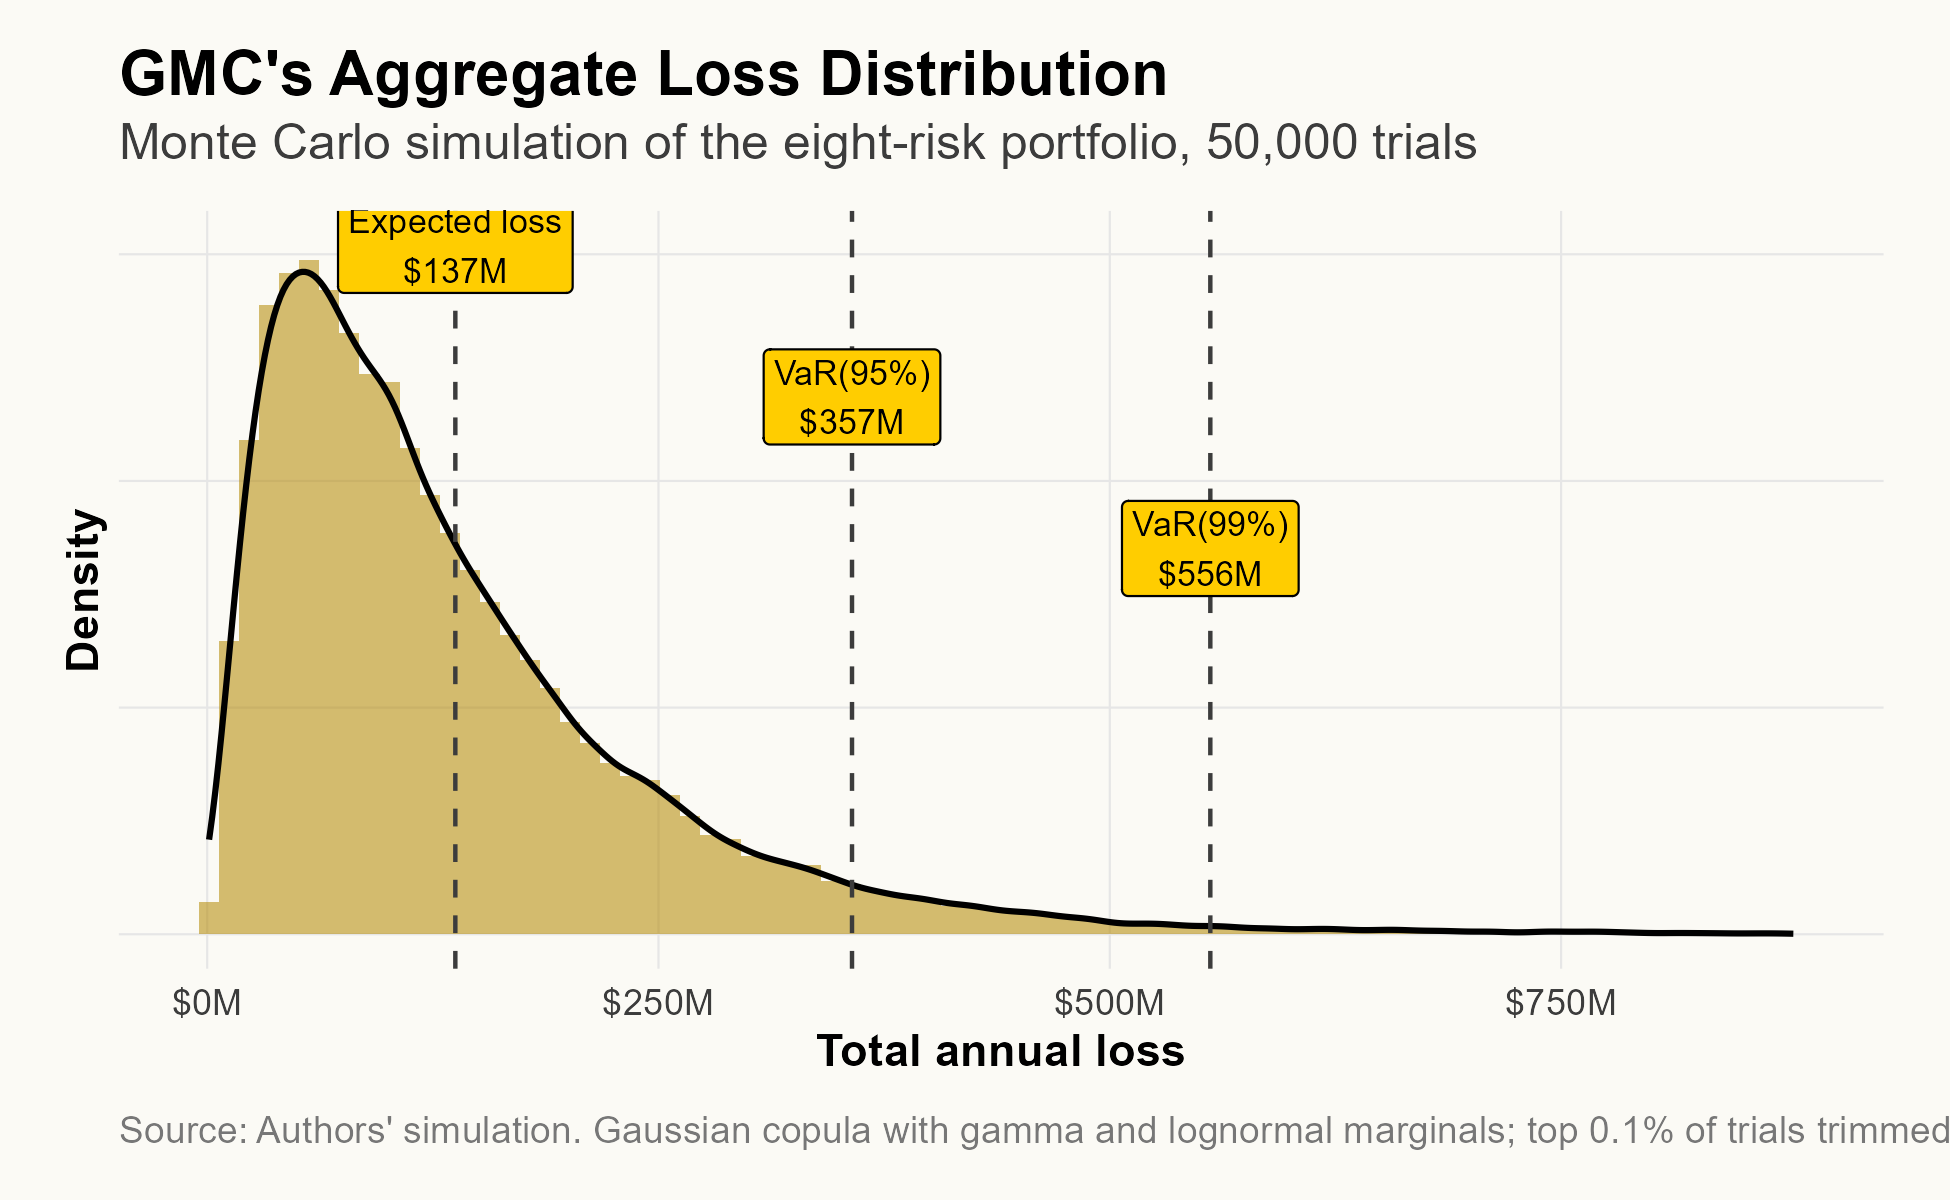
\includegraphics[width=\textwidth]{c6_aggregate_loss.png}
  \caption{GMC's simulated aggregate loss distribution. The distribution is
  strongly right-skewed: expected loss is \$137M, but VaR(95\%) is \$357M and
  VaR(99\%) is \$556M, well beyond what a normal approximation would predict.}
  \label{fig:gmc-aggregate}
  \figurenote{Monte Carlo simulation with 50{,}000 trials using a Gaussian
  copula on the correlation matrix in Table~\ref{tab:gmc-correlations}, with
  gamma marginals for most risks and lognormal marginals for supply chain and
  cyber risk. The top 0.1\% of trials is trimmed for display.}
\end{figure}

\subsection{Stress Testing}
\label{subsec:gmc-stress}

GMC designs three stress scenarios\index{stress testing}.

\textbf{Stress Scenario 1: Severe global recession.} Customer credit losses
triple (\$75M \(\rightarrow\) \$225M); commodity prices spike then collapse
(\$80M \(\rightarrow\) \$140M); strategic risk rises as customers cancel
contracts (\$70M \(\rightarrow\) \$120M); correlations among R1, R3, R8 rise
to 0.70. \textbf{Total portfolio loss: \$475M.}

\textbf{Stress Scenario 2: Major supply chain disruption.} Supply chain
disruption at the extreme---a geopolitical event (\$200M); property damage
from the same event (\$80M); product liability rises as substitute parts cause
defects (\$90M); cyber risk rises amid operational chaos (\$80M).
\textbf{Total portfolio loss: \$510M.}

\textbf{Stress Scenario 3: Combined moderate stress.} All risks at their 90th
percentiles---worse than expected, but no single catastrophe. \textbf{Total
portfolio loss: \$380M.}

\textbf{Conclusions:} under normal conditions (VaR(95\%) = \$352M), GMC is
within appetite. Under severe recession, losses (\$475M) exceed appetite and
consume nearly a quarter of equity. Under the supply chain crisis, losses
(\$510M) threaten covenant compliance. Even combined moderate stress (\$380M)
slightly exceeds appetite, though it is survivable.

\subsection{Management Actions and Portfolio Optimization}
\label{subsec:gmc-actions}

Portfolio analysis drives a concrete agenda.

\textbf{Risk mitigation:}
\begin{itemize}\tightlist
  \item Purchase additional property insurance with higher limits, capping R4
        at \$20M
  \item Expand the supplier diversification program, targeting a 20\%
        reduction in R6 VaR
  \item Increase commodity hedging (R3) to reduce volatility
\end{itemize}

\textbf{Capital and appetite:}
\begin{itemize}\tightlist
  \item Maintain current capital (\$2B equity) given the thin \$23M margin
        against the appetite limit
  \item Defer acquisition plans until portfolio risk falls---any new
        acquisition would push VaR above appetite
  \item Request board approval for a temporary appetite increase to \$425M if
        a strategic opportunity arises, with a 12-month plan to return
\end{itemize}

\textbf{Monitoring:}
\begin{itemize}\tightlist
  \item Quarterly portfolio VaR reporting to the board risk committee, with
        trend analysis
  \item Semi-annual stress testing with updated scenarios
  \item Ongoing monitoring of correlation changes
\end{itemize}

\textbf{Capital allocation and performance:}
\begin{itemize}\tightlist
  \item Allocate economic capital by marginal VaR contribution: Automotive
        45\% (\$540M), Industrial 35\% (\$420M), Consumer 20\% (\$240M)
  \item Measure RAROC per segment against a 12\% hurdle
  \item Include a risk-adjusted return metric in segment leaders' incentive
        compensation
\end{itemize}

\textbf{Result:} portfolio risk management transforms GMC's risk function from
a compliance exercise into a strategic tool informing capital allocation,
mitigation priorities, and growth decisions. The board sees its total risk
position relative to appetite---which is precisely what enterprise risk
management\index{enterprise risk management (ERM)} is for.

\begin{center}\rule{0.5\linewidth}{0.5pt}\end{center}

% -----------------------------------------------------------------------
\begin{keytakeaways}
\item
  A risk portfolio is the totality of material risks the firm faces,
  considered together with their interdependencies.
\item
  Total portfolio risk depends on individual risk magnitudes, correlations
  among risks, and the number of risks---it is not the sum of the parts.
\item
  Diversification reduces portfolio risk when correlations are less than
  perfect; benefits of 30--50\% relative to simple summation are typical.
\item
  Correlation (\(\rho\)) measures linear dependence between risks, ranging
  from \(-1\) to \(+1\); most business risk pairs fall between 0 and 0.6.
\item
  Risk aggregation methods include simple summation (conservative upper
  bound), variance-covariance (efficient, assumes normality), Monte Carlo
  simulation (flexible, handles skewed distributions), and copulas (capture
  tail dependence).
\item
  Correlations rise under stress; tail dependence means diversification is
  weakest exactly when it is needed most---as Maersk's NotPetya experience
  demonstrated, latent common dependencies can convert apparently independent
  exposures into one correlated loss.
\item
  Portfolio VaR, economic capital, and stress test results provide the
  enterprise-level metrics needed to assess compliance with board risk
  appetite.
\item
  Marginal contribution analysis identifies how much each risk or business
  unit adds to portfolio VaR, enabling rational capital allocation and
  risk-adjusted performance measurement (RAROC).
\item
  Stress testing complements probabilistic measures by evaluating extreme
  scenarios---historical, hypothetical, and reverse stress tests.
\item
  Implementation requires integrated data, correlation estimation discipline,
  model validation, and organizational commitment; the hardest problems are
  organizational, not mathematical.
\end{keytakeaways}

This chapter completes the core ERM technical toolkit: identify risks
(Chapter~3), quantify them individually (Chapter~4), establish appetite
(Chapter~5), and aggregate risks into portfolio views (Chapter~6). Subsequent
chapters explore risk response strategies and organizational implementation.

% -----------------------------------------------------------------------
\begin{keyterms}
  \item[\keyterm{Aggregate loss distribution}]
    The probability distribution of total losses across all risks in the
    portfolio, reflecting individual distributions and their correlations.
  \item[\keyterm{Copula}]
    A mathematical function separating the modeling of individual risk
    distributions from the modeling of dependencies, allowing flexible
    structures including tail dependence.
  \item[\keyterm{Correlation (\(\rho\))}]
    A statistical measure of the degree to which two variables move together,
    ranging from \(-1\) (perfect negative) to \(+1\) (perfect positive), with
    0 indicating independence.
  \item[\keyterm{Correlation matrix}]
    A table showing pairwise correlations between all risks in a portfolio,
    with diagonal elements equal to 1.
  \item[\keyterm{Covariance}]
    The expected value of the product of two variables' deviations from their
    means; Covariance(X,Y) = Correlation(X,Y) \(\times\) SD(X) \(\times\)
    SD(Y).
  \item[\keyterm{Diversification benefit}]
    The reduction in total portfolio risk relative to the simple sum of
    individual risks, arising from imperfect correlation.
  \item[\keyterm{Diversification ratio}]
    The ratio of portfolio risk to the sum of individual risks; values below 1
    indicate diversification benefit.
  \item[\keyterm{Economic capital}]
    The capital required to remain solvent at a specified confidence level
    given the firm's total risk portfolio.
  \item[\keyterm{Marginal VaR}]
    The incremental contribution of an individual risk to total portfolio
    VaR---portfolio VaR with the risk minus portfolio VaR without it.
  \item[\keyterm{Materiality threshold}]
    Criteria determining which risks are significant enough for the portfolio,
    based on financial magnitude, strategic importance, or regulatory
    requirements.
  \item[\keyterm{Monte Carlo simulation}]
    A computational technique generating thousands of random scenarios to
    construct empirical distributions of portfolio outcomes, accounting for
    risk distributions and correlations.
  \item[\keyterm{Portfolio VaR}]
    Value at Risk for the entire portfolio---the threshold loss exceeded with
    only a specified probability, accounting for diversification.
  \item[\keyterm{Reverse stress testing}]
    Working backwards from failure to identify what combination of events
    would cause it, then assessing plausibility.
  \item[\keyterm{Risk aggregation}]
    The process of combining individual risks to estimate total enterprise
    risk, accounting for correlations and dependencies.
  \item[\keyterm{Risk-Adjusted Return on Capital (RAROC)}]
    Net income divided by allocated economic capital, enabling return
    comparisons across units with different risk profiles.
  \item[\keyterm{Risk portfolio}]
    The totality of all material risks an organization faces, considered
    together as an integrated system including exposures and
    interdependencies.
  \item[\keyterm{Risk register}]
    A structured database documenting all material risks with identification,
    ownership, exposure metrics, correlations, and controls.
  \item[\keyterm{Stress testing}]
    Analysis evaluating portfolio performance under specific adverse scenarios
    that probabilistic measures may not capture.
  \item[\keyterm{Tail dependence}]
    The tendency for extreme losses across multiple risks to occur together
    more frequently than normal-period correlation predicts; correlations
    increase during crises.
  \item[\keyterm{Variance-covariance aggregation}]
    A method for calculating portfolio variance from individual risk variances
    and covariances (or correlations), based on portfolio theory.
\end{keyterms}

% -----------------------------------------------------------------------
\begin{discussionquestions}
\item \textbf{Conceptual:} Explain why examining risks individually rather
  than as a portfolio can lead to poor risk management decisions. Provide two
  specific examples of insights that portfolio analysis reveals that
  individual risk analysis misses.

\item \textbf{Conceptual:} Distinguish between correlation and tail
  dependence. Why does tail dependence matter for risk management even if
  normal-period correlations are low? How does the Maersk NotPetya case
  illustrate the distinction?

\item \textbf{Calculation:} Two risks each have expected loss of \$20M and
  standard deviation of \$10M. Calculate portfolio expected loss and standard
  deviation under three correlation assumptions: \(\rho = 1.0\),
  \(\rho = 0.5\), and \(\rho = 0\). Interpret the diversification benefit in
  each case.

\item \textbf{Application:} A company's current portfolio has VaR(95\%) =
  \$150M. The company is evaluating two potential acquisitions, each with
  standalone VaR(95\%) = \$50M. Acquisition~A correlates 0.8 with the current
  portfolio; Acquisition~B correlates 0.2. Without detailed calculations,
  explain qualitatively which acquisition adds more to portfolio risk and why.

\item \textbf{Integration:} Explain how portfolio VaR relates to risk appetite
  (Chapter~5). If a company's appetite is ``maximum annual loss shall not
  exceed \$200M with 95\% confidence,'' how does the company use portfolio
  analysis to assess compliance?

\item \textbf{Comparison:} Compare simple summation, variance-covariance
  aggregation, and Monte Carlo simulation as aggregation methods. What are the
  advantages and limitations of each? When is each most appropriate?

\item \textbf{Interpretation:} A company calculates portfolio VaR(95\%) =
  \$120M using the variance-covariance method and \$145M using Monte Carlo.
  What might explain the difference? Should management be concerned?

\item \textbf{Case analysis:} In the Global Manufacturing Co.\ case
  (Section~\ref{sec:gmc-case}), the diversification benefit was \$188M (35\%
  reduction). Identify three specific risk pairs with low correlation that
  contributed most to this benefit and explain why their correlation is low.

\item \textbf{Critical thinking:} A board member says ``If we have limited
  risk capacity, we should eliminate or reduce every risk as much as
  possible.'' Using portfolio concepts, explain why this reflects flawed
  reasoning. What should the board focus on instead?

\item \textbf{Strategy:} A manufacturing company operates only in the United
  States. Management proposes expansion into Europe and Asia. Using portfolio
  concepts, explain how this expansion might actually reduce total firm risk
  even though it adds new risks (foreign exchange, political, operational
  complexity). Under what conditions would expansion increase risk?

\item \textbf{Stress testing:} Design three stress test scenarios for a
  regional bank's risk portfolio. For each, identify which risks would be
  affected and how correlations might change under stress. Explain why these
  scenarios are more informative than relying solely on VaR.

\item \textbf{Organizational:} You are the newly appointed CRO of a company
  that has traditionally managed risks in functional silos (Treasury,
  Insurance, Operations). The CEO has asked you to implement portfolio risk
  management. Identify three major organizational or cultural challenges you
  expect and propose specific strategies to overcome each.
\end{discussionquestions}

% -----------------------------------------------------------------------
\begin{minicase}{Portfolio Risk Exercise --- TechRetail Corp}

\textbf{Scenario:} You are the risk analyst for \textbf{TechRetail Corp}, an
e-commerce and logistics company. The company has identified six material
risks (Table~\ref{tab:techretail-risks}) and estimated their correlations
(Table~\ref{tab:techretail-correlations}).

\begin{ermtable}{TechRetail's material risks}[tab:techretail-risks]
\begin{tabular}{@{}cllrr@{}}
\toprule
\textbf{ID} & \textbf{Risk Name} & \textbf{Expected Loss} &
\textbf{Std.\ Dev.} & \textbf{VaR(95\%)} \\
\midrule
R1 & Cyber/data breach        & \$15M & \$25M & \$60M \\
R2 & Warehouse accidents      & \$8M  & \$12M & \$28M \\
R3 & Delivery vehicle crashes & \$10M & \$15M & \$35M \\
R4 & Product liability        & \$12M & \$18M & \$42M \\
R5 & IT system failure        & \$5M  & \$10M & \$22M \\
R6 & Reputational damage      & \$7M  & \$20M & \$45M \\
\bottomrule
\end{tabular}
\end{ermtable}

\begin{ermtable}{TechRetail's correlation matrix}[tab:techretail-correlations]
\begin{tabular}{@{}lcccccc@{}}
\toprule
 & \textbf{R1} & \textbf{R2} & \textbf{R3} & \textbf{R4} & \textbf{R5} &
\textbf{R6} \\
\midrule
R1 & 1.00 & 0.15 & 0.10 & 0.20 & 0.70 & 0.60 \\
R2 & 0.15 & 1.00 & 0.40 & 0.30 & 0.10 & 0.20 \\
R3 & 0.10 & 0.40 & 1.00 & 0.50 & 0.10 & 0.25 \\
R4 & 0.20 & 0.30 & 0.50 & 1.00 & 0.15 & 0.70 \\
R5 & 0.70 & 0.10 & 0.10 & 0.15 & 1.00 & 0.50 \\
R6 & 0.60 & 0.20 & 0.25 & 0.70 & 0.50 & 1.00 \\
\bottomrule
\end{tabular}
\end{ermtable}

TechRetail's risk appetite: ``Portfolio VaR(95\%) shall not exceed \$180M.''

\medskip
\textbf{Part~1: Simple Aggregation (10 points).} Calculate total portfolio VaR
using simple summation (assuming perfect correlation). Does this exceed risk
appetite? By how much?

\medskip
\textbf{Part~2: Correlation Analysis (20 points).}
\begin{enumerate}[label=\alph*)]\tightlist
  \item Identify the two risks with the highest correlation. Explain
        intuitively why these risks might be highly correlated given
        TechRetail's business.
  \item Identify the two risks with the lowest correlation. Explain why these
        risks are largely independent.
  \item Based on the correlation matrix, which two risks offer the greatest
        diversification benefit when combined? Justify your answer.
\end{enumerate}

\medskip
\textbf{Part~3: Portfolio Calculation (30 points).} Using the
variance-covariance method:
\begin{enumerate}[label=\alph*)]\tightlist
  \item Calculate portfolio expected loss (simple sum of individual expected
        losses)
  \item Calculate portfolio variance using:
        \(\text{Portfolio Variance} = \sum \sigma_i^2 +
        \sum\sum \rho_{ij}\,\sigma_i\,\sigma_j\) for all \(i \neq j\)
  \item Calculate portfolio standard deviation =
        \(\sqrt{\text{Portfolio Variance}}\)
  \item Estimate portfolio VaR(95\%) using the normal approximation:
        VaR = Expected Loss + 1.645 \(\times\) Portfolio SD
\end{enumerate}
(Note: For the full calculation, use a spreadsheet or calculator. Show at
least the setup and a few sample calculations even if you don't compute the
final number by hand.)

\medskip
\textbf{Part~4: Diversification Benefit (20 points).}
\begin{enumerate}[label=\alph*)]\tightlist
  \item Calculate the diversification benefit: Simple Sum VaR \(-\) Portfolio
        VaR (from Parts~1 and~3)
  \item Calculate diversification benefit as a percentage:
        \([1 - (\text{Portfolio VaR} / \text{Simple Sum VaR})] \times 100\%\)
  \item Is the portfolio VaR within risk appetite? How much risk capacity
        remains?
\end{enumerate}

\medskip
\textbf{Part~5: Strategic Decision (20 points).} TechRetail is considering
launching same-day drone delivery. The new service would add:

R7: Drone accidents --- Expected Loss \$6M, Standard Deviation \$15M,
VaR(95\%) estimated \$35M

Estimated correlations with existing risks:
\begin{itemize}\tightlist
  \item R1 (Cyber): 0.40 (drones depend on IT systems, vulnerable to cyber)
  \item R2 (Warehouse): 0.25 (some connection through logistics operations)
  \item R3 (Vehicle crashes): 0.60 (both transportation risks)
  \item R4 (Product liability): 0.45 (drone accidents could damage products)
  \item R5 (IT failure): 0.55 (drones heavily IT-dependent)
  \item R6 (Reputational): 0.50 (drone accidents attract media attention)
\end{itemize}

Without performing full calculations, answer qualitatively:
\begin{enumerate}[label=\alph*)]\tightlist
  \item How do you expect R7 to affect portfolio VaR? Will it increase by the
        full \$35M standalone VaR, or by less due to diversification? Explain
        your reasoning with reference to the correlations.
  \item Should TechRetail approve the new service from a risk portfolio
        perspective if it offers attractive returns? What additional analysis
        would you recommend before a final decision?
\end{enumerate}

\medskip
\textbf{Submission format:} You may use Excel, a calculator, or show work by
hand. Submit calculations, answers, and written explanations (2--3 pages
total). Partial credit for methodology even if calculations contain errors.

\end{minicase}

% -----------------------------------------------------------------------
\section*{Advanced Challenge: Monte Carlo Portfolio Simulation}
\addcontentsline{toc}{section}{Advanced Challenge: Monte Carlo Portfolio Simulation}

For students comfortable with Excel or programming (R/Python):

\textbf{Task:} Build a Monte Carlo simulation for TechRetail's 6-risk
portfolio:

\begin{enumerate}\tightlist
  \item In Excel, create correlated normal random variables for the 6 risks
        using the Cholesky decomposition method or Excel's built-in
        correlation tools
  \item For each simulation trial (at least 1{,}000 trials), generate
        correlated losses for all 6 risks and sum to get total portfolio loss
  \item From the simulated portfolio losses: calculate the mean (portfolio
        expected loss), the standard deviation (portfolio SD), and the 95th
        percentile (portfolio VaR(95\%)); create a histogram of the portfolio
        loss distribution
  \item Compare your Monte Carlo results to the variance-covariance results
        from the main exercise
  \item Write a brief summary (1 page) discussing: How closely do Monte Carlo
        and variance-covariance results agree? What are the advantages of
        Monte Carlo for this problem? How would you modify the simulation to
        better capture tail risk?
\end{enumerate}

\textbf{Optional extension:} Introduce non-normal distributions (e.g.,
lognormal for R1 cyber risk to capture right-skew) and observe how the
portfolio distribution changes.

% -----------------------------------------------------------------------
\section*{References}
\addcontentsline{toc}{section}{References}
\begingroup
\sloppy

\begin{hangparas}{1.5em}{1}

Columbia University School of International and Public Affairs. (2022).
\emph{NotPetya: A Columbia University case study.} Columbia SIPA.
\url{https://www.sipa.columbia.edu/sites/default/files/2022-11/NotPetya%20Final.pdf}

Committee of Sponsoring Organizations of the Treadway Commission. (2017).
\emph{Enterprise risk management---Integrating with strategy and performance.}
COSO. \url{https://www.coso.org/}

Greenberg, A. (2018a, August 22). The untold story of NotPetya, the most
devastating cyberattack in history. \emph{WIRED}.
\url{https://www.wired.com/story/notpetya-cyberattack-ukraine-russia-code-crashed-the-world/}

Greenberg, A. (2018b, February 15). The White House blames Russia for
NotPetya, the ``most costly cyberattack in history.'' \emph{WIRED}.
\url{https://www.wired.com/story/white-house-russia-notpetya-attribution/}

International Organization for Standardization. (2018). \emph{ISO~31000:2018
Risk management---Guidelines} (2nd~ed.). ISO.
\url{https://www.iso.org/standard/65694.html}

Los Angeles Times. (2017, August 17). Maersk cyberattack closes Port of Los
Angeles terminal. \emph{Los Angeles Times}.
\url{https://www.latimes.com/business/la-fi-maersk-cyberattack-20170817-story.html}

Markowitz, H. (1952). Portfolio selection. \emph{The Journal of Finance,
7}(1), 77--91.

\end{hangparas}

\endgroup
\end{document}

% !TeX root = Chapter_07_Loss_Control_Risk_Reduction.tex
% Chapter 7 — Loss Control and Risk Reduction
\documentclass[11pt,openany]{book}
\usepackage{graphicx}
\usepackage{amsmath,amssymb}
\usepackage{hanging}
\makeatletter
\def\input@path{{second_ed/style/}{../style/}}
\makeatother
\usepackage{erm_textbook_style}
\providecommand{\tightlist}{\setlength{\itemsep}{0pt}\setlength{\parskip}{0pt}}
\emergencystretch=2em

\begin{document}

\setcounter{chapter}{6}
\chapter{Loss Control and Risk Reduction}
\label{chap:loss-control}

% -----------------------------------------------------------------------
\begin{learningobjectives}
  \item Explain the frequency-severity framework and how loss control
        interventions target each component independently or in combination.
  \item Calculate the expected return on investment (ROI) of loss control
        investments using pre-control and post-control frequency and severity
        data.
  \item Apply the hierarchy of controls framework (elimination
        \(\rightarrow\) substitution \(\rightarrow\) engineering
        \(\rightarrow\) administrative \(\rightarrow\) PPE) to analyze
        workplace hazards and select optimal control strategies.
  \item Design loss control programs tailored to different industry
        environments including manufacturing, retail, construction, and
        healthcare operations.
  \item Measure loss control effectiveness using standard metrics including
        Total Recordable Incident Rate (TRIR), Days Away/Restricted/Transfer
        Rate (DART), and Experience Modification Rate (EMR).
  \item Evaluate tradeoffs between risk financing (insurance, retention) and
        risk reduction (loss control investment) using total cost of risk
        analysis.
  \item Integrate loss control decisions with the risk appetite and portfolio
        management frameworks from Chapters~5 and~6.
\end{learningobjectives}

% -----------------------------------------------------------------------
\chapteroverview{%
The first six chapters of this book were mostly about understanding risk:
naming it, measuring it, deciding how much of it the organization can stand,
and seeing how individual exposures combine into a portfolio. This chapter is
about changing it. Loss control---the systematic application of techniques to
reduce the frequency and severity of losses---is the point in the ERM cycle
where analysis turns into physical and procedural intervention: a machine
guard, a sprinkler head, a permit system, a sensor in a hallway outlet.

The economics are the heart of the chapter, and they are surprisingly
favorable. Well-chosen loss control investments routinely return several
hundred percent annually with payback periods under a year, yet they often
face more skepticism in capital budgeting than production investments with far
weaker returns. We develop the tools to make the case rigorously: the total
cost of risk framework, frequency-severity ROI analysis, and the NIOSH
hierarchy of controls for choosing among interventions. Industry cases from
manufacturing, retail, construction, and healthcare show the same logic
working in very different hazard environments, and a set of standard metrics
(TRIR, DART, EMR) lets you verify whether a program actually worked rather
than merely sounding good.

A theme runs through the chapter: loss control does not just shrink expected
losses---it reshapes the entire loss distribution that Chapters~4 and~6 taught
you to analyze. The opening case shows an insurer doing exactly that, one
small plastic device at a time. An appendix at the end of the chapter develops
the full financial theory---discounting, taxes, insurance pricing dynamics,
real options, and portfolio effects---for readers who want to see how the
simplified ROI model connects to corporate finance.%
}

\clearpage

% -----------------------------------------------------------------------
% Opening Corporate Example: Crestline Mutual
% -----------------------------------------------------------------------
\begin{corporateexample}[Crestline Mutual and the House That Didn't Burn]

On a hot July afternoon, the Collins house looked like every other two-story
in the subdivision---vinyl siding, a small porch, a swing in the backyard.
Behind the walls, the wiring carried twenty years of changes: a do-it-yourself
ceiling fan, an extra outlet in the garage, holiday lights that had once
pushed a circuit harder than the builder intended. The lights still worked and
the breakers hadn't tripped in months. If you had asked Mark Collins about
fire risk, he would have pointed to the grill on the deck. The wires in the
walls felt like background---unseen, assumed sound.

At Crestline Mutual\index{Crestline Mutual}, his home insurer, those same houses showed up
differently. On the company's loss reports, electrical fires in single-family
homes were a stubborn line: not the most frequent cause of loss, but
disproportionately severe when they appeared. For years Crestline had managed
the risk the usual ways---higher rates for older homes, discounts for smoke
alarms, the occasional inspector with a clipboard noting extension cords under
rugs. Then a small technology vendor arrived with a different pitch: instead
of pricing around electrical-fire risk, what if Crestline could help prevent
the fires?

The device was simple to look at---a box the size of a night-light that
plugged into an ordinary outlet and ``listened'' to the home's electrical
system, analyzing subtle patterns in current and voltage that signal arcing,
loose connections, or failing equipment before visible signs appear. The
actuarial team asked for data. In a large multi-year pilot with other
carriers, across more than a million home-years of experience, homes with the
devices had measurably fewer electrical-fire claims than a matched control
group---and the devices had led electricians to dozens of serious faults that
likely would have become fires. It was not a magic shield, but it was one of
the few loss-control ideas that came to the table with measured reductions in
both the probability of loss and, in some cases, the size of losses when fires
still occurred. Crestline launched its own program in several states where
electrical-fire severity ran high.

Mark and his wife accepted the free ``smart fire-prevention'' benefit by
email, plugged the device into a hallway outlet, and forgot about it. One
Sunday evening in October, Mark's phone buzzed: the system had detected
repeated arcing events on a circuit feeding the garage. The lights weren't
flickering; the breakers were fine; it was easy to think ``spam.'' But the
follow-up call from the monitoring service was specific enough to feel
serious. Two days later, an electrician pulled a receptacle free behind the
workbench and found one terminal charred, the plastic cracked, the wood in the
box darkened. Years earlier someone had back-stabbed the wires into the
outlet, and the connection had loosened over time. ``This,'' he said, holding
it up, ``is the kind of thing that smolders for a while before it lights
something up.'' The repair took less than an hour. Crestline covered part of
the bill.

When Crestline's analysts later compared loss experience between participating
homes and a control group, the divergence they had hoped for began to emerge.
Electrical-fire claims still happened---randomness had not disappeared---but
they were less frequent in houses with the devices, and a higher share of the
fires that did occur were contained to a room or a single appliance instead of
consuming the structure. The shape of the loss distribution was changing, not
because Crestline had written different words in a policy form, but because
the underlying risk in thousands of homes was slightly, measurably safer. In
the annual planning deck, the program appeared as a line item: an investment
in technology and service, a modest shift in expected loss costs. In
neighborhoods like the Collins', it looked quieter---a small device glowing in
a hallway outlet, occasionally catching the moment when a hidden fault can
still be fixed with a screwdriver and a new outlet instead of a fire truck and
an adjuster.

\source{Insurance Information Institute, \emph{The Efficacy and Return on
Investment of Loss Prevention Programs: Background, Methods, and Results}
(2025); Whisker Labs loss-prevention program data.}
\end{corporateexample}

% =======================================================================
\section{From Risk Identification to Risk Reduction}
\label{sec:loss-control-imperative}

\subsection{The Loss Control Imperative}

In Chapters~3 through~6 we focused on understanding and measuring risk:
identifying risk categories, quantifying frequency and severity distributions,
setting risk appetite thresholds, and analyzing how individual risks aggregate
into enterprise-level exposures. That work is essential, but it is only half
of the ERM equation. A risk register, however carefully quantified, never
prevented a fire. Once an organization understands its risks, it must decide
what to do about them.

The traditional ERM risk response framework offers four options: avoid,
reduce, transfer, or accept (COSO, 2017). Risk avoidance\index{risk avoidance}---simply not engaging
in activities that create risk---is occasionally appropriate but often means
forgoing profitable business. Risk transfer\index{risk transfer} through insurance and contracts
moves financial consequences to third parties, at a cost and often with
limited coverage for the worst scenarios. Risk acceptance\index{risk acceptance}---consciously
retaining risk within appetite boundaries---is necessary for risks that cannot
be economically avoided, reduced, or transferred. This chapter focuses on the
remaining response: risk reduction through loss control.

Loss control\index{loss control} encompasses all activities designed to reduce either the
frequency (likelihood) of loss events or the severity (magnitude) of losses
when events occur. Unlike risk transfer, which shifts financial consequences
after losses materialize, loss control changes the underlying physical and
operational reality so that losses happen less often or do less damage. The
Crestline program in the opening case is a clean example: the insurer did not
reprice the risk or rewrite the policy form---it changed the probability that
a loose terminal becomes a structure fire. Effective loss control programs
deliver benefits well beyond direct loss reduction: lower insurance premiums
through improved experience ratings, better operational efficiency, stronger
employee morale and retention, improved regulatory compliance, reduced
litigation exposure, and protection of brand reputation (Occupational Safety
and Health Administration [OSHA], 2016).

\subsection{Loss Control in the ERM Framework}

Loss control decisions must be integrated with the broader ERM framework
established in prior chapters. An organization's risk appetite\index{risk appetite}---the amount
and type of risk it is willing to accept in pursuit of objectives
(Chapter~5)---directly influences loss control priorities. Risks that fall
outside appetite boundaries demand aggressive control measures regardless of
whether the controls clear an ROI hurdle; risks comfortably within tolerance
may require only monitoring and basic preventive practices. Recall from
Chapter~5 that appetite becomes genuinely operational only after
identification and quantification mature---loss control is where that maturity
pays off, because a firm that knows its loss distributions can target control
spending where appetite is binding.

Portfolio effects also matter. In Chapter~6 we saw how risks correlate and
aggregate---and how a single event like NotPetya at Maersk can ripple across
what looked like independent exposures. Loss control investments should
prioritize high-severity risks and risks that correlate strongly with other
exposures, since controlling these delivers both direct benefits and
diversification improvements to the overall portfolio. A manufacturing
facility fire is a hazard risk with direct property damage, but it also
triggers business interruption losses (operational), potential customer
contract penalties (financial), and possible regulatory scrutiny if
environmental releases occur (strategic/reputational). Preventing that fire
through sprinkler systems and hot-work permits creates value across multiple
risk categories simultaneously.

The quantification tools from Chapter~4 provide the analytical foundation.
Frequency-severity data, loss distributions, and Value at Risk (VaR)\index{Value at Risk (VaR)}
calculations let organizations estimate the expected financial benefit of
proposed controls and compare it to implementation cost. This cost-benefit
discipline transforms loss control from an intuitive ``safety is good''
platitude into a capital allocation decision that can be defended in the same
room, with the same rigor, as any other investment.

% =======================================================================
\section{The Economics of Loss Control}
\label{sec:loss-control-economics}

\subsection{The Total Cost of Risk Framework}

Organizations often view risk management costs narrowly, focusing on insurance
premiums and large retained losses. This limited perspective obscures the true
economic impact of risk and leads to suboptimal decisions. The total cost of
risk (TCOR)\index{total cost of risk (TCOR)} framework provides a comprehensive view by summing all
risk-related expenditures and opportunity costs (Risk and Insurance Management
Society [RIMS], 2008):\footnote{Total cost of risk calculations vary by
organization and methodology. RIMS provides comprehensive guidance in the
\emph{RIMS Benchmark Survey} published annually. Organizations should develop
consistent TCOR definitions to enable valid year-over-year comparisons.}

\[
\begin{split}
\text{Total Cost of Risk} = {}& \text{Direct Losses} + \text{Loss Control Costs}
  + \text{Risk Transfer Costs} \\
  & + \text{Administrative Costs} + \text{Indirect Costs}
\end{split}
\]

Where:

\begin{itemize}\tightlist
  \item \textbf{Direct Losses} = retained losses not covered by insurance
        (deductibles, self-insured retentions, uninsured losses)
  \item \textbf{Loss Control Costs} = engineering improvements, safety
        equipment, training programs, inspections, safety personnel
  \item \textbf{Risk Transfer Costs} = insurance premiums, letters of credit,
        surety bonds, contractual risk transfer costs
  \item \textbf{Administrative Costs} = risk management department salaries,
        consultants, claims adjusters, legal defense
  \item \textbf{Indirect Costs} = business interruption, productivity losses,
        damaged reputation, opportunity costs, employee morale impacts
\end{itemize}

For many organizations, the total cost of risk runs from 1\% to 5\% of
revenue, with higher percentages in hazard-intensive industries such as
construction, transportation, and manufacturing (RIMS, 2008). Notice the
structure of the tradeoff: loss control appears as a cost in the framework but
simultaneously reduces direct losses, lowers risk transfer costs (through
better insurance pricing), and shrinks indirect costs (through fewer
disruptions). The goal is to minimize TCOR, not to minimize any single
component---a point that matters when a CFO asks why the safety budget is
growing.

\subsection{Loss Control Return on Investment}
\label{subsec:loss-control-roi}

Loss control investments should be evaluated with the same financial
discipline applied to other capital expenditures. The expected annual benefit
equals the reduction in expected losses plus any reduction in insurance
premiums or other risk costs:

\[
\begin{split}
\text{Annual Benefit} = {}& (\text{Pre-Control Expected Loss} -
  \text{Post-Control Expected Loss}) \\
  & + \text{Premium Savings} + \text{Indirect Benefit}
\end{split}
\]

Expected loss, as introduced in Chapter~4, equals the product of frequency and
severity. Loss control can reduce either or both components:

\[
\text{Expected Loss} = \text{Frequency} \times \text{Average Severity}
\]

Simple return on investment (ROI)\index{return on investment (ROI)} compares annual benefits to the control
investment:

\[
\text{ROI} = \frac{\text{Annual Benefit} - \text{Annualized Control Cost}}
  {\text{Annualized Control Cost}}
\]

And simple payback period\index{payback period} measures how long it takes for cumulative benefits
to recover the initial investment:

\[
\text{Payback Period} = \frac{\text{Initial Investment}}{\text{Annual Benefit}}
\]

Consider a warehouse operation experiencing forklift-pedestrian collisions at
a frequency of 8 incidents per year with an average cost of \$12{,}000 per
incident (medical expenses, lost time, equipment damage, OSHA penalties).
Pre-control expected annual loss is \(8 \times \$12{,}000 = \$96{,}000\). The
risk manager proposes installing pedestrian barriers, high-visibility
markings, and proximity warning systems at a cost of \$45{,}000, combined with
annual refresher training costing \$3{,}000. Based on industry data and vendor
specifications, these controls are expected to reduce incident frequency by
75\% (to 2~incidents per year) and average severity by 30\% (to \$8{,}400 per
incident) due to lower-speed collisions and improved emergency response.

Post-control expected annual loss \(= 2 \times \$8{,}400 = \$16{,}800\).
Annual loss reduction \(= \$96{,}000 - \$16{,}800 = \$79{,}200\). Annualized
control cost \(= (\$45{,}000\,/\,\text{10-year equipment life}) + \$3{,}000
\text{ annual training} = \$7{,}500\). Annual ROI
\(= (\$79{,}200 - \$7{,}500)\,/\,\$7{,}500 = 956\%\). Simple payback period
\(= \$45{,}000\,/\,\$79{,}200 = 0.57\) years (approximately 7~months). An
investment returning over nine times its annual cost, while also protecting
employees and reducing regulatory exposure, would be extraordinary anywhere
else in the capital budget. In loss control, it is not unusual.

The same arithmetic scales up. Crestline's\index{Crestline Mutual} fire-prevention program was, at
bottom, this calculation run across thousands of homes: device and monitoring
costs per household on one side; reduced fire frequency, reduced fire
severity, and avoided claim-adjustment expense on the other. The insurer's
advantage was a portfolio large enough to make the loss reductions
statistically visible---a luxury the single warehouse above does not have,
which is why industry data and vendor studies, not just internal experience,
inform the frequency and severity assumptions.

\subsection{Diminishing Returns and Optimal Investment}

Loss control investments typically exhibit diminishing marginal returns\index{diminishing returns}. The
first safety improvements---eliminating the most obvious hazards, addressing
the highest-frequency incidents---deliver substantial loss reduction per
dollar invested. As an organization moves toward more sophisticated or
comprehensive controls, each incremental dollar yields progressively smaller
reductions. Eventually, additional loss control spending exceeds the
achievable benefit, and resources should shift to other risk management
strategies.

The optimal loss control investment level minimizes total cost of risk. Too
little investment leaves the organization exposed to preventable losses and
high insurance premiums. Too much consumes resources that could create value
elsewhere. This optimization must consider not only direct financial returns
but also regulatory requirements (which set minimum control standards), risk
appetite constraints (which may mandate controls even for
low-frequency/high-severity risks that fail traditional ROI tests), and
stakeholder expectations regarding employee safety and community
responsibility. The appendix to this chapter develops this optimization
formally, including the time value of money, tax effects, and the option value
of deferring or expanding control programs.

% =======================================================================
\section{Frequency Reduction Techniques}
\label{sec:frequency-reduction}

\subsection{The Logic of Frequency Control}

Frequency reduction\index{frequency reduction} aims to decrease the number of loss events during a given
time period. In the frequency-severity framework from Chapter~4, frequency
control shifts the loss count distribution leftward, reducing the mean number
of events while ideally not affecting the severity distribution (how large
losses are when they occur). Frequency control is particularly valuable for
high-frequency, low-severity risks where the cumulative impact of many small
losses creates significant cost and operational disruption. It is also the
half of the Crestline story that worked through early warning: the device's
alerts converted incipient fires into electrician visits, removing events from
the loss count entirely.

From a safety management perspective, many frequency reduction techniques
focus on preventing the unsafe acts and unsafe conditions that create loss
potential. The U.S. Bureau of Labor Statistics reports that in 2022, private
industry employers reported approximately 2.7~million nonfatal workplace
injuries and illnesses, or 2.7~cases per 100 full-time workers (U.S. Bureau of
Labor Statistics [BLS], 2023a). While this represents improvement from
historical levels, the economic burden remains substantial when considering
both direct costs (medical, compensation) and indirect costs (productivity,
morale, training replacements). Effective frequency reduction systematically
addresses the precursors to these incidents.

\subsection{Engineering-Based Frequency Reduction}

Engineering controls\index{engineering controls} physically prevent hazardous events from occurring by
eliminating the opportunity for human error or equipment failure to create
loss. Examples include:

\textbf{Machine Guarding.}\index{machine guarding} Physical barriers that prevent worker contact with
dangerous machine components such as rotating shafts, cutting blades, or pinch
points. OSHA\index{OSHA} requires machine guarding under 29~CFR~1910.212, and properly
designed guards can eliminate most machine-contact injuries without reducing
productivity (OSHA, 2007).

\textbf{Interlocks and Fail-Safes.} Devices that prevent equipment operation
unless safe conditions exist. A punch press that requires two-hand activation
ensures both hands are away from the danger zone; an emergency stop button
immediately de-energizes equipment when pressed. Industrial robots often use
light curtains that stop motion if broken by a body part entering the danger
zone.

\textbf{Automatic Safety Systems.} Fire suppression systems that activate
without human intervention, emergency shutdown systems that respond to
abnormal conditions, and ventilation systems that maintain safe atmospheric
conditions. The National Fire Protection Association (NFPA) reports that
automatic sprinkler systems activate in 88\% of fires large enough to trigger
them and control or extinguish the fire in 96\% of these activations,
dramatically reducing both fire frequency and severity (NFPA, 2021).

\textbf{Physical Separation.} Barriers, guardrails, and bollards that separate
workers from hazardous areas or prevent vehicle-pedestrian conflicts.
Warehouse operations commonly use bollard posts to protect structural columns
and create safe pedestrian walkways separated from forklift traffic lanes.

\subsection{Procedural and Administrative Frequency Reduction}
\label{subsec:admin-frequency}

Administrative controls\index{administrative controls} establish rules, procedures, and work practices that
reduce loss frequency by standardizing safe behaviors and requiring deliberate
assessment before high-risk activities:

\textbf{Lockout/Tagout (LOTO).}\index{lockout/tagout (LOTO)} Procedures that ensure machinery is properly
shut down and isolated from energy sources before maintenance or servicing,
preventing unexpected startup that could injure workers. OSHA's Control of
Hazardous Energy standard (29~CFR~1910.147) requires LOTO programs for
equipment with hazardous energy sources. OSHA estimates LOTO compliance
prevents approximately 120 fatalities and 50{,}000 injuries annually (OSHA,
2002).

\textbf{Permit Systems.}\index{permit systems} Hot work permits (for welding, cutting, grinding),
confined space entry permits, excavation permits, and similar authorization
procedures that require hazard assessment, preparation, and monitoring before
high-risk work begins. Permits force deliberate planning and often require
multiple approvals, reducing the likelihood that workers proceed into
dangerous situations unprepared.

\textbf{Pre-Task Planning and Job Safety Analysis (JSA).}\index{job safety analysis (JSA)} Structured processes
where work teams analyze tasks, identify hazards, and agree on control
measures before beginning work. JSA breaks complex jobs into steps, examines
hazards at each step, and specifies safe procedures and required personal
protective equipment (PPE).

\textbf{Inspection and Audit Programs.} Regular workplace inspections identify
emerging hazards before they cause losses. Effective inspection programs
combine scheduled comprehensive audits with ongoing informal observations by
supervisors and safety committees. Leading organizations empower all employees
to report hazards and near-miss incidents without fear of blame, creating an
early-warning system for frequency control.

\subsection{Training and Competency Development}

Training\index{safety training} ensures workers understand hazards, recognize high-risk situations,
and possess the knowledge and skills to perform tasks safely. OSHA requires
training for numerous specific hazards including hazardous materials (Hazard
Communication Standard, 29~CFR~1910.1200), powered industrial trucks
(forklifts, 29~CFR~1910.178), fall protection, and confined spaces (OSHA,
2015).

Effective training goes beyond annual classroom sessions to include hands-on
practice, job-specific mentoring, and regular refreshers. Forklift operator
certification, for example, requires both classroom instruction on safety
principles and practical driving exercises demonstrating proficiency in
maneuvering, load handling, and emergency procedures. Research consistently
demonstrates that well-trained workers experience lower injury frequencies
than untrained or poorly trained peers performing similar work (NIOSH, 2015).

Training effectiveness depends on reinforcement through supervision and safety
culture. Organizations with strong safety cultures---where leadership visibly
prioritizes safety, workers feel comfortable reporting hazards, and safe
practices are consistently recognized---achieve lower injury frequencies than
organizations that view safety as merely regulatory compliance (OSHA, 2016).
This cultural dimension of frequency control complements technical and
procedural measures by shaping the day-to-day decisions that either prevent or
create loss opportunities.

% =======================================================================
\section{Severity Control Strategies}
\label{sec:severity-control}

\subsection{The Logic of Severity Control}

Severity control\index{severity control} aims to reduce the magnitude of loss when an adverse event
occurs. While frequency control prevents events from happening, severity
control accepts that some events are inevitable and focuses on limiting their
damage. In the frequency-severity framework, severity controls compress the
severity distribution, reducing both the average loss and the tail risk
(extreme losses) without necessarily affecting how often events occur. The
Crestline data showed this signature clearly: among participating homes, fires
still occurred, but a higher share were contained to a room or a single
appliance---the right tail of the severity distribution had been pulled in.

Severity control is especially valuable for low-frequency, high-severity
risks---the catastrophic exposures that threaten organizational viability.
Natural disasters, major fires, large liability claims, and catastrophic
equipment failures may be difficult to prevent entirely (low frequency-control
leverage) but often can be contained or mitigated through planning,
redundancy, and rapid response (high severity-control leverage). Insurance
actuaries and risk managers often focus on maximum foreseeable loss (MFL)\index{maximum foreseeable loss (MFL)} or
probable maximum loss (PML)\index{probable maximum loss (PML)}---estimates of worst-case scenarios---when
designing severity controls for property, business interruption, and liability
exposures.

\subsection{Property Damage Severity Control}

For physical property exposures, severity control focuses on limiting fire
spread, containing hazardous material releases, and protecting critical
assets:

\textbf{Automatic Sprinkler Systems.}\index{automatic sprinkler systems} As noted in Section~3.2, sprinklers
dramatically reduce fire severity. NFPA data indicate that sprinklers reduce
the average property loss per fire by 60\% to 70\% compared to unsprinklered
buildings, and civilian fire deaths are 87\% lower in sprinklered buildings
(NFPA, 2021). Sprinklers exemplify dual-purpose controls: they provide modest
frequency reduction (some small fires are extinguished immediately) and
substantial severity reduction (major fires are controlled until firefighters
arrive).

\textbf{Fire-Resistant Construction and Compartmentation.} Fire-rated walls,
doors, and floor-ceiling assemblies slow fire spread, allowing time for
evacuation and suppression. Compartmentation divides large buildings into
smaller fire-rated sections, preventing a fire originating in one area from
destroying the entire facility. Building codes typically require increasing
levels of fire resistance for larger buildings, higher occupancies, and
structures storing hazardous materials.

\textbf{Separation of High-Value Property.} Distributing critical assets
across multiple locations reduces the maximum possible loss from any single
event. A manufacturer might maintain inventory in several regional warehouses
rather than one central facility, ensuring that a fire or natural disaster at
one location does not eliminate all inventory and halt all production. Data
centers routinely establish geographically separated backup facilities to
ensure business continuity if the primary site is destroyed.

\textbf{Secondary Containment and Spill Control.} For operations involving
hazardous materials, secondary containment systems (berms, dikes, double-walled
tanks) prevent spills from spreading beyond the immediate area and
contaminating soil, groundwater, or surface water. Environmental cleanup costs
often dwarf the value of the spilled material itself, making containment
highly cost-effective severity control. The U.S. Environmental Protection
Agency's Spill Prevention, Control, and Countermeasure (SPCC) regulations
require containment systems for oil storage facilities (40~CFR Part~112).

\subsection{Injury Severity Control}

For occupational injuries, severity control minimizes the physical harm and
financial cost when incidents occur:

\textbf{Emergency Medical Response.} Immediate access to first aid, automated
external defibrillators (AEDs), and trained emergency responders reduces
injury severity by providing rapid treatment during the critical first minutes
after an incident. The American Heart Association reports that immediate CPR
and defibrillation can increase survival rates for sudden cardiac arrest by
50\% or more (American Heart Association, 2020). Workplaces with trained first
responders and well-stocked medical supplies typically experience shorter
disability durations and lower medical costs per injury.

\textbf{Early Return-to-Work Programs.}\index{return-to-work programs} Modified-duty and transitional work
programs allow injured workers to return to productive activity before full
recovery, reducing wage replacement costs and preventing the physical
deconditioning and psychological distress associated with prolonged work
absence. Workers' compensation research consistently shows that early
return-to-work programs reduce claim durations by 30\% to 50\% and improve
long-term recovery outcomes (National Council on Compensation Insurance
[NCCI], 2017).

\textbf{Claims Management and Medical Cost Containment.}\index{claims management} Active management of
injury claims---prompt reporting, selection of appropriate medical providers,
case management for serious injuries, fraud detection---significantly reduces
workers' compensation severity. Organizations with dedicated claims
professionals and preferred provider networks typically achieve 20\% to 30\%
lower medical costs per claim than organizations with passive claims handling
(NCCI, 2017).

\textbf{Personal Protective Equipment (PPE).}\index{personal protective equipment (PPE)} While PPE is the least effective
control in the hierarchy (Section~\ref{sec:hierarchy}), it provides important
severity reduction when engineering and administrative controls cannot fully
eliminate exposure. Hard hats reduce traumatic brain injury severity, safety
glasses prevent eye injuries, hearing protection limits noise-induced hearing
loss, and cut-resistant gloves reduce laceration severity. The key limitation
of PPE is that it requires consistent proper use by individual workers, making
it vulnerable to human error and unsuitable as the primary control for serious
hazards.

\subsection{Business Interruption Severity Control}

Physical damage often triggers business interruption\index{business interruption}---the inability to
operate and generate revenue. Business interruption severity can exceed direct
property damage costs, particularly for businesses with high fixed costs,
time-sensitive operations, or contracts with penalty clauses for
non-performance. Recall from Chapter~6 how NotPetya turned a single malware
infection into a fleet-wide operational shutdown at Maersk: the direct damage
was to software, but the severity came from the interruption. Controls
include:

\textbf{Redundancy and Backup Systems.} Duplicate production equipment, backup
power generators, redundant information technology systems, and alternative
suppliers allow operations to continue or resume quickly after disruptions.
The cost of redundancy must be weighed against both the likelihood and
consequences of interruption. High-revenue operations with thin margins often
justify substantial redundancy investment; lower-revenue operations may accept
greater interruption risk. Maersk's post-NotPetya investments in network
segmentation and recovery capacity are severity controls in exactly this
sense---they would not prevent the next infection, but they would contain it.

\textbf{Emergency Response and Business Continuity Planning.}\index{business continuity planning} Pre-established
plans, trained response teams, and regular drills enable organizations to
mobilize quickly when disruptions occur, minimizing downtime duration.
Effective plans identify critical functions, prioritize recovery sequences,
pre-position necessary resources, and establish clear command structures and
communication protocols. Organizations with tested business continuity plans
typically resume operations two to three times faster than organizations
attempting ad hoc recovery (Federal Emergency Management Agency [FEMA], 2021).

\textbf{Supply Chain Diversification.}\index{supply chain diversification} Dependence on sole-source suppliers
creates vulnerability to interruption if that supplier experiences production
problems, quality failures, natural disasters, or financial distress.
Qualifying alternative suppliers and maintaining relationships with backup
vendors adds administrative cost but dramatically reduces business
interruption severity when primary suppliers fail. Chapter~6's portfolio
analysis flagged supply chain concentration as a correlated operational risk
deserving priority attention; supplier diversification is the loss control
response to that finding.

% =======================================================================
\section{Engineering Controls and Physical Safeguards}
\label{sec:engineering-controls}

\subsection{Machine Guarding and Point-of-Operation Protection}

Machine-related injuries have declined significantly since OSHA began
enforcing machine guarding requirements in the 1970s, but powered machinery
remains a major source of workplace injuries. OSHA's machine guarding
standards (29~CFR~1910.212) require that ``one or more methods of machine
guarding shall be provided to protect the operator and other employees in the
machine area from hazards such as those created by point of operation, ingoing
nip points, rotating parts, flying chips and sparks'' (OSHA, 2007).

Effective guards must prevent workers from reaching into danger zones while
allowing necessary material feeding, operation, and maintenance. Common guard
types include:

\textbf{Fixed Guards.} Permanent barriers that require tools for removal,
suitable for operations with consistent material handling. Sheet metal guards
over belt drives, chain drives, and gear mechanisms exemplify fixed guarding.

\textbf{Interlocked Guards.} Movable guards connected to machine controls, so
the machine cannot operate unless the guard is closed, and the machine stops
if the guard opens during operation. Interlocked guards allow access for setup
and maintenance while preventing exposure during powered operation.

\textbf{Adjustable Guards.} Guards that accommodate varying material sizes,
common on woodworking machinery like table saws and band saws. Operators
adjust the guard for each operation, requiring training and discipline to
maintain protection.

\textbf{Self-Adjusting Guards.} Guards that automatically accommodate
different material sizes by moving out of the way when material passes, then
returning to the protective position. Woodworking and metalworking machines
often use self-adjusting guards to balance protection with operational
flexibility.

Point-of-operation guarding specifically protects the area where material
processing occurs---where the cutting, forming, bending, or assembling action
happens. Power presses and similar equipment require especially robust
point-of-operation protection due to their extreme hazard. Common solutions
include two-hand control systems (requiring both hands on control buttons,
ensuring hands are away from the danger zone), light curtains (photoelectric
sensors that stop the machine if the light beam is broken), and
pull-back/restraint devices (physical mechanisms that pull the operator's
hands away from the danger zone when the machine cycles).

\subsection{Electrical Safety Controls}

Electrical hazards cause approximately 120 worker deaths and thousands of
non-fatal injuries annually in the United States (BLS, 2023b). Electrical
safety controls focus on preventing shock, electrocution, and electrical
fires:

\textbf{Ground Fault Circuit Interrupters (GFCIs).} Devices that detect
current imbalances indicating electrical leakage (which may be flowing through
a person's body) and immediately interrupt power. OSHA requires GFCIs on
construction sites and in other environments where workers may contact
electrical equipment with wet conditions or grounded surfaces
(29~CFR~1926.404). GFCIs prevent fatal electrocution from ground faults,
reducing shock deaths by more than 50\% where deployed (OSHA, 2016).

\textbf{Lockout/Tagout for Electrical Work.} As discussed in
Section~\ref{subsec:admin-frequency}, LOTO procedures ensure electrical
equipment is de-energized and cannot be re-energized unexpectedly before
workers perform maintenance, reducing electrocution risk during servicing.

\textbf{Insulation and Guarding of Energized Parts.} Electrical panels,
switchgear, and conductors must be insulated or enclosed to prevent accidental
contact. OSHA's electrical standards (29~CFR~1910, Subpart~S) specify required
clearances, warning signs, and training for workers who may be exposed to
energized electrical parts.

\textbf{Arc Flash Protection.} High-amperage electrical equipment can create
explosive arc flash events releasing intense heat, light, and pressure. Arc
flash risk assessment, equipment labeling, proper arc-rated PPE, and safe work
practices reduce arc flash injury severity. The National Fire Protection
Association's NFPA~70E standard provides comprehensive guidance for electrical
safety in workplaces (NFPA, 2021).

The monitoring technology in the opening case belongs to this family.
Continuous waveform analysis is, in effect, an engineering control for a
hazard that traditional controls reach only at inspection intervals: it
watches the electrical system between inspections and converts a slow,
invisible deterioration into an actionable alert.

\subsection{Fall Protection Systems}

Falls from elevation cause the most construction worker
deaths---approximately 350 fatalities annually---and thousands of serious
injuries across all industries (BLS, 2023b). OSHA requires fall protection\index{fall protection}
when workers are exposed to falls of six feet or more in construction
(29~CFR~1926.501) and four feet or more in general industry (29~CFR~1910.23).
Fall protection approaches include:

\textbf{Guardrails.} Passive systems (requiring no worker action) consisting
of top rails, mid-rails, and toe boards that physically prevent falls from
open edges, floor openings, and elevated platforms. Guardrails provide the
most reliable protection because they do not depend on individual worker
compliance.

\textbf{Personal Fall Arrest Systems.} Full-body harnesses connected via
lanyards or lifelines to secure anchor points. If a fall occurs, the system
arrests the fall within a short distance, preventing impact with lower levels.
Fall arrest systems require proper training, daily inspection, and careful
attention to anchorage strength and fall clearance calculations. They are less
preferable than guardrails because they rely on consistent proper use.

\textbf{Fall Restraint Systems.} Similar to fall arrest but designed to
prevent the worker from reaching the fall hazard by limiting travel distance.
Restraint systems avoid the shock load and injury potential of actual fall
arrest but require precise setup for the specific work location.

\textbf{Safety Nets.} Nets positioned beneath elevated work areas to catch
falling workers. Nets are commonly used in steel erection and bridge
construction where guardrails and personal systems are impractical. Nets must
meet strength and mesh size requirements and be positioned close enough
beneath work areas to limit fall distance.

For ground-level work, slip-and-fall prevention focuses on housekeeping
(keeping floors clean, dry, and free of obstacles), appropriate flooring
materials (non-slip surfaces in wet areas), adequate lighting, proper
footwear, and immediate cleanup of spills. Slip-and-fall claims represent a
major liability exposure for retail stores, restaurants, hotels, and other
public accommodations.

% =======================================================================
\section{Administrative Controls and Behavioral Interventions}
\label{sec:admin-controls}

\subsection{Safety Culture and Leadership Engagement}

Engineering controls and physical safeguards provide the foundation for loss
control, but organizational culture determines whether those controls are
consistently maintained and whether workers follow safe practices in
situations where engineering solutions alone cannot eliminate risk. Safety
culture\index{safety culture}---the shared values, beliefs, and norms regarding safety that
characterize an organization---has emerged as a critical factor distinguishing
low-injury from high-injury organizations performing similar work (OSHA,
2016).\footnote{OSHA's Voluntary Protection Programs (VPP) recognize employers
with exemplary safety management systems. VPP sites demonstrate comprehensive
implementation of hierarchy controls, systematic measurement, and sustained
performance typically 50\% better than industry average.}

Research consistently identifies leadership commitment as the strongest
predictor of safety culture. When senior executives visibly prioritize safety,
allocate resources to safety initiatives, participate in safety activities,
and hold managers accountable for safety performance, workers perceive safety
as a genuine organizational value rather than regulatory compliance theater.
Conversely, when leaders emphasize production and cost reduction while giving
safety only rhetorical support, workers correctly conclude that safety is
secondary and adjust their behavior accordingly.

Effective safety leadership practices include executive safety walks (visible
presence in operational areas, asking workers about hazards and listening to
concerns), regular safety performance reviews at board and executive meetings
(examining leading and lagging indicators in detail), linking compensation to
safety outcomes for managers and executives (making safety a financial
incentive, not just production), and celebrating safety achievements
(recognizing individuals and teams who identify hazards, implement
improvements, or sustain incident-free performance).

\subsection{Behavioral Safety Programs}

Behavioral safety programs\index{behavioral safety programs} systematically observe worker behaviors, provide
feedback, and reinforce safe practices. The underlying premise is that unsafe
behaviors (taking shortcuts, failing to use PPE, disabling guards, proceeding
without proper preparation) precede many injuries, and modifying these
behaviors reduces injury frequency. Behavioral safety techniques include:

\textbf{Safety Observations.} Trained observers watch workers performing
tasks, note safe and unsafe behaviors using standardized checklists, and
provide immediate non-punitive feedback. Observation data is aggregated to
identify patterns and prioritize interventions. The emphasis is on
understanding why workers choose unsafe behaviors (time pressure, inadequate
tools, poor ergonomics, lack of knowledge) rather than simply blaming
individuals.

\textbf{Near-Miss Reporting Systems.}\index{near-miss reporting} Programs that encourage workers to
report close calls---situations where an injury or property damage nearly
occurred but didn't---without fear of discipline. Near-misses typically
outnumber actual injuries by ratios of 10:1 or higher, providing a much larger
dataset for identifying and correcting hazardous conditions and behaviors
before injuries result. Heinrich's Safety Triangle\index{Heinrich's Safety Triangle}, though its specific ratios
are debated, illustrates the concept: many unsafe conditions and behaviors
(the triangle base) lead to fewer minor injuries (middle), which occasionally
escalate to serious injuries or fatalities (tip) (NIOSH,
2015).\footnote{The Heinrich Safety Triangle has been challenged by modern
research suggesting ratios vary by industry and that near-misses do not always
predictably precede serious injuries. Nonetheless, near-miss reporting
provides valuable hazard intelligence even if specific ratios are uncertain.}

\textbf{Positive Reinforcement.} Recognizing and rewarding safe behaviors,
hazard reporting, and safety suggestions. Positive reinforcement creates
cultural momentum toward safety by making safety engagement visible and
valued. Recognition can range from verbal praise and certificates to safety
awards, prizes, or financial bonuses for sustained safe performance.

\textbf{Safety Committees and Worker Involvement.} Worker participation in
safety committees, hazard assessments, and improvement projects gives
employees voice in safety decisions and taps their frontline knowledge of
risks and practical solutions. OSHA actively encourages worker participation
in safety programs and views worker engagement as a key element of effective
safety management systems (OSHA, 2016).

\subsection{Leading and Lagging Indicators}
\label{subsec:leading-lagging}

Organizations measure safety performance using both lagging indicators\index{lagging indicators}
(outcomes that have occurred) and leading indicators\index{leading indicators} (proactive activities
that predict future outcomes). Sole reliance on lagging indicators creates two
problems: they reflect past performance and may not predict future risk, and
in organizations with low injury frequency, lagging indicators provide sparse
data, making performance trends difficult to identify.

\textbf{Lagging indicators} include:

\begin{itemize}\tightlist
  \item \textbf{Total Recordable Incident Rate (TRIR):}\index{Total Recordable Incident Rate (TRIR)} number of
        OSHA-recordable injuries and illnesses per 100 full-time workers
        annually. TRIR = (number of recordable cases \(\times\) 200{,}000) /
        total hours worked by all employees. The 200{,}000 constant represents
        100 workers working 40~hours per week for 50~weeks.
  \item \textbf{Days Away, Restricted, or Transferred (DART) rate:}\index{DART rate} subset of
        TRIR focusing on more serious cases involving days away from work,
        restricted duty, or job transfer. DART = (number of DART cases
        \(\times\) 200{,}000) / total hours worked.
  \item \textbf{Lost workday rate:} days of work lost due to injury or illness
        per 100 full-time workers.
  \item \textbf{Experience Modification Rate (EMR):}\index{Experience Modification Rate (EMR)} workers' compensation
        insurance modifier comparing an organization's actual losses to
        expected losses for similar organizations. EMR = 1.0 is average;
        EMR \(<\) 1.0 indicates better-than-average experience; EMR \(>\) 1.0
        indicates worse-than-average. EMR directly affects insurance premiums
        (NCCI, 2017).
\end{itemize}

\textbf{Leading indicators} include training hours per employee and the
percentage of workers current on required training, the number of safety
observations completed, near-miss reports submitted per employee, hazards
identified and corrected through inspections, safety suggestion participation
rates, the percentage of pre-task planning forms completed, permit compliance
rates, and time to hazard correction after identification.

Leading indicators enable proactive management by revealing process weaknesses
before injuries occur. Organizations with mature safety programs typically
track balanced scorecards incorporating both leading and lagging indicators,
recognizing that investment in leading activities (training, inspections,
maintenance) drives lagging results (lower injury rates, lower costs). The
Crestline program had exactly this structure: anomalies flagged and faults
corrected were the leading indicators; fire claims, months later, were the
lagging confirmation.

% =======================================================================
\section{The Hierarchy of Controls Framework}
\label{sec:hierarchy}

\subsection{NIOSH Hierarchy of Controls}

The National Institute for Occupational Safety and Health (NIOSH)\index{NIOSH} hierarchy of
controls\index{hierarchy of controls} provides a systematic framework for selecting the most effective
control measures for workplace hazards. The hierarchy ranks control options
from most to least effective, based on how reliably they reduce risk and how
vulnerable they are to human error or equipment failure (NIOSH, 2015):

\textbf{1. Elimination.}\index{hierarchy of controls!elimination} Physically remove the hazard entirely. If a hazardous
material is not present, or a hazardous process is not performed, the risk
disappears. Elimination provides absolute protection and requires no ongoing
maintenance or worker compliance. Example: a manufacturer eliminates
hexavalent chromium exposure by reformulating paint to remove chromium
compounds. Elimination is the ideal control but often infeasible for core
production processes.

\textbf{2. Substitution.}\index{hierarchy of controls!substitution} Replace a hazardous material, process, or equipment
with a less hazardous alternative. Substitution reduces risk without
eliminating the work activity. Example: substituting water-based solvents for
volatile organic compound (VOC) solvents reduces fire, health, and
environmental risks while maintaining cleaning effectiveness. Substitution
requires careful analysis to ensure the replacement does not introduce new
hazards.

\textbf{3. Engineering Controls.}\index{hierarchy of controls!engineering controls} Isolate people from hazards using physical
barriers, ventilation, automation, or equipment redesign. Engineering controls
reduce risk without relying on worker behavior change. Examples: machine
guards, local exhaust ventilation capturing welding fumes, automated material
handling replacing manual lifting, enclosed processes preventing exposure to
hazardous chemicals. Engineering controls are highly reliable because they
function passively or automatically.

\textbf{4. Administrative Controls.}\index{hierarchy of controls!administrative controls} Modify work procedures, training,
rotation, or scheduling to reduce exposure. Administrative controls depend on
information, training, and discipline. Examples: job rotation to reduce
repetitive motion exposure, lockout/tagout procedures, hot work permits,
reduced shift length in hot environments. Administrative controls are less
reliable than engineering controls because they require consistent human
compliance.

\textbf{5. Personal Protective Equipment (PPE).}\index{hierarchy of controls!personal protective equipment (PPE)} Provide equipment worn by
workers to shield them from hazards. PPE is the last line of defense because
it does not reduce the hazard itself and depends entirely on proper selection,
fit, maintenance, and consistent use by individual workers. Examples: safety
glasses, hearing protection, respirators, gloves, protective clothing, fall
arrest harnesses. PPE is appropriate as supplementary protection or when
higher-level controls are infeasible, but should not be the primary control
for serious hazards.

\subsection{Applying the Hierarchy in Practice}

The hierarchy guides control selection by directing attention first to the
most effective options. When evaluating control strategies for a specific
hazard, risk managers and safety professionals should systematically consider
each level of the hierarchy, preferably implementing controls from multiple
levels to create defense-in-depth\index{defense-in-depth}.

\textbf{Example: Controlling Noise Exposure in a Manufacturing Facility.}
A stamping press generates 95~dBA noise, exceeding OSHA's 90~dBA action level
(29~CFR~1910.95). Workers exposed to this noise face hearing loss risk.
Applying the hierarchy:

\emph{Elimination:} Can the stamping process be eliminated? If stamping is
essential for production, elimination is infeasible.

\emph{Substitution:} Can a quieter alternative process produce equivalent
parts? If hydraulic presses are significantly quieter than mechanical presses
for this application, substitution may be economically viable during equipment
replacement cycles. Can different materials or part designs reduce stamping
noise?

\emph{Engineering controls:} Can the press be enclosed in a sound-dampening
structure? Can vibration damping materials be added to dies and structure? Can
the press be relocated farther from workers, or workers relocated farther from
the press? Engineering controls reducing press noise to below 85~dBA would
eliminate the hazard for most workers.

\emph{Administrative controls:} Can worker exposure time be limited through
job rotation, reducing cumulative noise dose below action levels? Can
maintenance schedules and equipment upgrades prioritize noise reduction? Can
high-noise work be scheduled for times when fewer workers are present?
Administrative controls provide partial protection but require ongoing
management attention.

\emph{PPE:} Hearing protection (earplugs or earmuffs) attenuates noise
reaching workers' ears. If higher-level controls reduce noise to 90~dBA, PPE
can provide the additional 5~dBA reduction to reach safe levels. PPE alone
would require workers to wear protection consistently throughout exposure,
making enforcement and training critical. Many organizations use PPE as backup
protection even when engineering controls are in place, creating redundant
defense.

The comprehensive solution might include some engineering controls
(enclosures, damping materials), administrative controls (maintenance
procedures, high-noise-area signage), and PPE (hearing protection required in
designated high-noise zones), illustrating defense-in-depth combining multiple
hierarchy levels.

\subsection{Economic Considerations in Hierarchy Application}

Higher-hierarchy controls (elimination, substitution, engineering) typically
require larger upfront investments but deliver more reliable, permanent risk
reduction with lower ongoing costs. Lower-hierarchy controls (administrative,
PPE) usually have lower upfront costs but require sustained expenditures for
training, monitoring, replacement, and enforcement. The hierarchy thus aligns
technical effectiveness with long-term economics: the most effective controls
often prove most economical over equipment lifecycles or multi-year periods.

OSHA regulations embody hierarchy principles by requiring feasible engineering
and administrative controls before relying on PPE. For example, OSHA's
respiratory protection standard (29~CFR~1910.134) states ``the employer shall
use engineering controls and work practices to reduce and maintain employee
exposure to respiratory hazards to within the limits specified\ldots when such
controls are not feasible or while they are being instituted, the employer
shall provide respirators.'' This regulatory framework prevents employers from
choosing inexpensive PPE when more effective controls are feasible.

% =======================================================================
\section{Loss Control in Different Industries}
\label{sec:industries}

The hierarchy and the ROI arithmetic are general; the hazards are not. This
section works through four industry cases---manufacturing, retail,
construction, and healthcare---using the same analytical template each time:
establish the baseline frequency and severity, design controls, estimate the
post-control profile, and compute the return. Watch how the ROI varies across
settings, and why even the lowest figure still clears any reasonable hurdle
rate.

\subsection{Manufacturing: Machine Guarding ROI}
\label{subsec:mercer}

\textbf{Mercer Tool \& Stamping, Inc.}\index{Mercer Tool and Stamping} operates a 150-employee metal
fabrication facility producing precision-machined components for aerospace and
automotive customers. Over a three-year period, the company experienced
18~machine-related injuries ranging from minor lacerations to a serious hand
injury requiring hospitalization and reconstructive surgery. Total direct
costs (workers' compensation medical and indemnity payments) reached
\$287{,}000, and estimated indirect costs (supervisor time, investigations,
training replacements, production disruption, OSHA recordkeeping) added
approximately \$340{,}000, for combined costs of \$627{,}000 over three years,
or \$209{,}000 annually.

The safety manager conducted a comprehensive hazard assessment identifying
14~machines with inadequate guarding: lathes, mills, punch presses, grinders,
and saws. Many guards had been removed or modified to facilitate material
loading and never reinstalled, or were original equipment that did not meet
current standards. Working with a machine guarding specialist, the company
developed a \$125{,}000 capital improvement program including:

\begin{itemize}\tightlist
  \item Installation of interlocked barrier guards on punch presses
        (\$32{,}000)
  \item Light curtain point-of-operation protection on two large presses
        (\$28{,}000)
  \item Fixed guarding for rotating shafts, pulleys, and belts on legacy
        equipment (\$18{,}000)
  \item Adjustable blade guards on table saws and band saws (\$12{,}000)
  \item Training program on guard use and maintenance (\$15{,}000)
  \item Annual guard inspection and maintenance program (\$20{,}000 initial
        cost; \$8{,}000 annually thereafter)
\end{itemize}

The CFO questioned whether this investment was justified, particularly during
a year of tight capital budgets. The safety manager prepared a cost-benefit
analysis.

\textbf{Pre-control frequency:} 18 incidents / 3~years = 6 per year.
\textbf{Expected post-control frequency:} industry data and vendor studies
suggest comprehensive guarding reduces machine contact injuries by 80--90\%.
Conservative estimate: \(6 \times 0.20 = 1.2\) incidents per year.

\textbf{Pre-control average severity:} \$287{,}000 / 18 incidents
\(\approx\) \$15{,}944 medical/indemnity per incident. Including indirect
costs: (\$287{,}000 + \$340{,}000) / 18 \(\approx\) \$34{,}833 total per
incident.
\textbf{Expected post-control severity:} remaining incidents are likely less
severe (minor cuts rather than amputations) due to improved guarding.
Estimated severity reduction: 40\%. Post-control severity:
\(0.60 \times (\$627{,}000 / 18) = \$20{,}900\) per incident.

\textbf{Expected annual loss reduction} (working from the exact three-year
totals to avoid rounding error):
\begin{align*}
\text{Pre-control:} \quad & \$627{,}000 / 3 = \$209{,}000 \\
\text{Post-control:} \quad & 1.2 \times \$20{,}900 = \$25{,}080 \\
\text{Annual savings:} \quad & \$209{,}000 - \$25{,}080 = \$183{,}920
\end{align*}

\textbf{Annualized control cost:} capital investment amortized over the
10-year expected equipment life: \$125{,}000 / 10 = \$12{,}500; annual
maintenance \$8{,}000; total annual cost \$20{,}500.

\textbf{ROI calculation:}
\begin{align*}
\text{Annual ROI} &= (\$183{,}920 - \$20{,}500)\,/\,\$20{,}500 = 797\% \\
\text{Simple payback period} &= \$125{,}000\,/\,\$183{,}920 = 0.68
  \text{ years (approximately 8 months)}
\end{align*}

The CFO approved the investment, recognizing both the financial return and the
organizational responsibility to protect workers. Three years
post-implementation, the company had experienced only one machine-related
injury (a minor laceration requiring first aid), compared to the predicted
3.6~incidents over that period, suggesting actual performance exceeded the
conservative projection. Workers' compensation EMR improved from 1.24 to 0.89,
reducing annual premiums by \$67{,}000---a benefit not included in the
original analysis. The company also used the improved safety record in
marketing to aerospace customers requiring supplier safety certifications.
(The appendix to this chapter revisits this case with full after-tax NPV
analysis, showing that even the impressive 797\% simple ROI understates the
value created.)

\subsection{Retail: Slip-and-Fall Prevention}
\label{subsec:midtown}

\textbf{Midtown Foods}\index{Midtown Foods}, a regional supermarket chain with 22 stores, faced
escalating slip-and-fall\index{slip-and-fall prevention} liability claims. Over five years, the company
averaged 18 customer slip-and-fall claims per year with an average settled
cost of \$32{,}000 per claim (combining small settlements for minor injuries,
larger settlements for serious fractures, and allocated defense costs). Total
annual slip-fall cost: \(18 \times \$32{,}000 = \$576{,}000\). General
liability insurance premiums had increased 40\% over three years due to poor
loss experience.

The risk manager analyzed claim data, identifying three primary causes:
(1)~entrance areas during wet weather (47\% of claims), (2)~the produce
department where fruit and vegetable spillage created slippery floors (28\% of
claims), and (3)~customer restrooms (14\% of claims). Armed with this
analysis, the risk manager developed a \$180{,}000 loss control program
implemented over two years:

\textbf{Entrance improvements (\$95{,}000):}
\begin{itemize}\tightlist
  \item Commercial-grade entrance matting systems extending 15~feet into
        vestibules and store interiors, capturing moisture from shoes
  \item Roof extensions creating covered outdoor areas, reducing water
        tracking
  \item Floor dryers and wet-floor signage protocols during wet weather
  \item Entrance inspection checklist requiring hourly checks during rain/snow
\end{itemize}

\textbf{Produce department improvements (\$45{,}000):}
\begin{itemize}\tightlist
  \item Anti-fatigue rubber mats with drainage holes in high-spill areas
        behind produce counters
  \item Rapid spill response protocol: employees carry radio-dispatched spill
        kits; response target 2~minutes
  \item Elimination of bulk grape displays (highest spillage product);
        pre-packaged grapes only
  \item Increased cleaning frequency from twice daily to four times daily
        during peak hours
\end{itemize}

\textbf{Restroom improvements (\$25{,}000):}
\begin{itemize}\tightlist
  \item Non-slip floor tiles replacing ceramic tiles during scheduled restroom
        renovations
  \item Hand dryer upgrades reducing water on floors from dripping hands
  \item Hourly restroom inspections with signed checklists
\end{itemize}

\textbf{Training and culture (\$15{,}000):}
\begin{itemize}\tightlist
  \item Employee training emphasizing spill response, hazard awareness, and
        customer service recovery after incidents
  \item Monthly safety meetings reviewing slip-fall incidents and control
        effectiveness
  \item Incentive program for stores with zero slip-fall claims over a quarter
\end{itemize}

Note the hierarchy at work: the grape decision is elimination (the hazard is
simply gone), the matting and flooring are engineering controls, and the
inspection checklists are administrative---defense-in-depth rather than
reliance on any single layer.

Results after two years: post-control frequency of 8 claims per year (down
from 18, a 56\% reduction) and post-control severity of \$28{,}000 per claim
(down from \$32{,}000, a 13\% reduction due to quicker responses limiting fall
severity and early settlement negotiations reducing defense costs).

\begin{align*}
\text{Pre-control annual loss:} \quad & 18 \times \$32{,}000 = \$576{,}000 \\
\text{Post-control annual loss:} \quad & 8 \times \$28{,}000 = \$224{,}000 \\
\text{Annual savings:} \quad & \$352{,}000
\end{align*}

Annualized control cost: capital amortized over 10 years (\$18{,}000) plus
ongoing annual cost for additional cleaning labor and inspections
(\$22{,}000), totaling \$40{,}000.

\begin{align*}
\text{ROI} &= (\$352{,}000 - \$40{,}000)\,/\,\$40{,}000 = 780\% \\
\text{Payback} &= \$180{,}000\,/\,\$352{,}000 = 0.51
  \text{ years (approximately 6 months)}
\end{align*}

The insurance carrier recognized the improvements by reducing general
liability premiums 22\% at the next renewal (approximately \$95{,}000 annual
premium savings)---an additional benefit beyond direct loss reduction. Over
the five-year period following program implementation, Midtown Foods averaged
only 7 claims per year with average cost of \$26{,}000, sustaining the
improvement and validating the control investments.

\subsection{Construction: Fall Protection Systems}
\label{subsec:summit}

Falls from elevation cause more construction worker deaths than any other
hazard---approximately 350 fatalities annually in the United States,
representing one-third of all construction deaths (BLS, 2023b).
\textbf{Summit Commercial Builders}\index{Summit Commercial Builders}, a 220-employee commercial contractor,
faced both regulatory pressure from OSHA citations for fall protection
violations and rising workers' compensation costs from non-fatal fall
injuries.

Over three years, the company experienced 24 fall-related workers'
compensation claims (averaging 8~per year) with costs ranging from \$8{,}000
for minor sprains requiring physical therapy to \$385{,}000 for a fall from a
second-story deck resulting in spinal injuries and permanent disability.
Average cost per fall claim: \$58{,}000. Additionally, OSHA citations for fall
protection violations totaled \$247{,}000 in fines over the three-year period.
Combined annual costs: \((8 \times \$58{,}000) + (\$247{,}000 / 3) =
\$546{,}000\) annually.

The company's safety director proposed a comprehensive fall protection program
requiring \$340{,}000 investment over two years:

\textbf{Equipment purchase (\$185{,}000):}
\begin{itemize}\tightlist
  \item Personal fall arrest systems (harnesses, lanyards, self-retracting
        lifelines) for all workers exposed to elevation hazards
  \item Guardrail systems (temporary railing for slab edges, roof edges)
  \item Ladder safety cages and stabilizers
  \item Mobile elevated work platforms (scissor lifts, aerial lifts) replacing
        extension ladder use for repetitive work
\end{itemize}

\textbf{Training and competent person development (\$95{,}000):}
\begin{itemize}\tightlist
  \item OSHA 10-hour and 30-hour construction safety training for all workers
        and supervisors
  \item Specialized fall protection competent person training for
        15~supervisors qualified to evaluate fall hazards, select appropriate
        protection, and oversee installation
  \item Annual fall protection refresher training
  \item Training on proper inspection and use of fall arrest equipment
\end{itemize}

\textbf{Administrative systems (\$60{,}000):}
\begin{itemize}\tightlist
  \item Fall protection plans required for each project, identifying elevation
        hazards and specifying control measures
  \item Pre-task planning incorporating fall hazard assessment for every task
  \item Daily equipment inspection program with documentation
  \item Incentives for supervisors and crews maintaining fall protection
        compliance
\end{itemize}

Results after full two-year implementation: post-control frequency of 2.5 fall
claims per year (down from 8, a 69\% reduction); post-control severity of
\$42{,}000 per claim (down from \$58{,}000, a 28\% reduction reflecting fewer
high-elevation falls and improved incident response); and zero fall protection
citations in the subsequent three years.

\begin{align*}
\text{Pre-control annual loss:} \quad & \$546{,}000 \\
\text{Post-control annual loss:} \quad & (2.5 \times \$42{,}000) + \$0
  \text{ citations} = \$105{,}000 \\
\text{Annual savings:} \quad & \$441{,}000
\end{align*}

Annualized control cost: capital amortized over 7~years of equipment useful
life (\$340{,}000 / 7 = \$48{,}571) plus ongoing annual costs for training,
equipment maintenance, and administrative time (\$35{,}000), totaling
\$83{,}571.

\begin{align*}
\text{ROI} &= (\$441{,}000 - \$83{,}571)\,/\,\$83{,}571 = 428\% \\
\text{Payback} &= \$340{,}000\,/\,\$441{,}000 = 0.77
  \text{ years (approximately 9 months)}
\end{align*}

Beyond direct financial returns, Summit Commercial Builders used the improved
safety record in pre-qualification for major projects. Many sophisticated
building owners and construction managers now require contractors to
demonstrate safety performance (TRIR, EMR, OSHA citation history) during
bidding. Summit's safety improvements qualified the company for larger,
higher-margin institutional and industrial projects previously inaccessible,
creating strategic value exceeding the direct loss control ROI.

\subsection{Healthcare: Workplace Violence Prevention}
\label{subsec:hospital}

Healthcare workers face elevated workplace violence\index{workplace violence prevention} risk, particularly in
emergency departments, psychiatric units, and long-term care facilities. The
U.S. Bureau of Labor Statistics reports that healthcare and social assistance
workers experience workplace violence injuries at rates four times higher than
private-sector averages (BLS, 2023a). \textbf{Community Regional Medical
Center}\index{Community Regional Medical Center}, a 425-bed hospital, experienced increasing workplace violence
incidents including patient-on-staff assaults, threats, and aggressive
behavior.

Analysis of five years of incident reports revealed 142 reportable workplace
violence incidents (averaging 28 per year) resulting in 37 workers'
compensation injuries (averaging 7.4 per year). While many incidents caused no
physical injury, they created substantial indirect costs: staff turnover,
security responses, police reports, incident investigations, counseling
services, and decreased employee morale. Direct workers' compensation costs
for violence-related injuries averaged \$18{,}000 per claim. Estimated total
annual cost including direct and indirect: \$350{,}000.

The hospital implemented a comprehensive violence prevention program over
18~months at a cost of \$425{,}000:

\textbf{Environmental design (\$215{,}000):}
\begin{itemize}\tightlist
  \item Emergency department redesign: curved reception desk preventing
        patients from cornering staff, panic buttons at all workstations,
        reinforced security glass at triage
  \item Psychiatric unit improvements: anti-ligature fixtures, secure
        medication rooms, breakaway door hinges
  \item Improved lighting in parking areas and external pathways
  \item Furniture selection emphasizing items difficult to weaponize
\end{itemize}

\textbf{Staff training (\$115{,}000):}
\begin{itemize}\tightlist
  \item De-escalation techniques training for all patient-contact staff,
        teaching verbal strategies to reduce patient agitation
  \item Restraint team training for specialized response to violent situations
  \item Threat recognition and situational awareness training
  \item Active shooter and lockdown drills
\end{itemize}

\textbf{Administrative controls and response (\$95{,}000):}
\begin{itemize}\tightlist
  \item Violence risk screening at patient admission, flagging patients with
        violence history
  \item Security officer presence in the emergency department during
        high-volume hours
  \item Buddy system for patient care in high-risk situations
  \item Post-incident support program including counseling, time off, incident
        review
  \item Incident reporting system capturing all violence events (not just
        injuries) to enable pattern analysis
\end{itemize}

Results after full implementation: total incidents decreased to 16 per year
(43\% reduction); workers' compensation injuries decreased to 3.2 per year
(57\% reduction); and severity fell to \$14{,}500 per claim (a 19\% reduction
reflecting less severe injuries from better de-escalation and response).

\begin{align*}
\text{Pre-control annual loss:} \quad & \$350{,}000 \\
\text{Post-control annual loss:} \quad & (3.2 \times \$14{,}500) +
  \$120{,}000 \text{ indirect} = \$166{,}400 \\
\text{Annual savings:} \quad & \$183{,}600
\end{align*}

Annualized control cost: capital amortized over 10~years (\$42{,}500) plus
annual ongoing cost for training, security, and program coordination
(\$48{,}000), totaling \$90{,}500.

\begin{align*}
\text{ROI} &= (\$183{,}600 - \$90{,}500)\,/\,\$90{,}500 = 103\% \\
\text{Payback} &= \$425{,}000\,/\,\$183{,}600 = 2.3 \text{ years}
\end{align*}

While this ROI is lower than the manufacturing or retail examples, hospital
leadership viewed the program as successful given the difficulty of
quantifying intangible benefits: improved staff retention (avoiding nursing
turnover costs of \$40{,}000+ per RN), enhanced hospital reputation, the
ethical duty to provide a safe work environment, and reduced liability
exposure for employee injury claims. Employee satisfaction survey scores for
``hospital takes safety seriously'' improved from 61\% to 84\%
agree/strongly agree, suggesting culture benefits beyond measurable injury
reduction. The comparison with the earlier cases is instructive: a 103\% ROI
would be a celebrated outcome in most corporate capital budgets, yet it is the
\emph{weakest} result in this section---a reminder of how unusual loss control
economics are.

% =======================================================================
\section{Measuring Loss Control Effectiveness}
\label{sec:measurement}

If Chapter~4's Moneyball lesson was that disciplined measurement beats
intuition, loss control is where the lesson gets applied to safety. A program
that cannot demonstrate its effect in the numbers is indistinguishable from a
program that has no effect. This section covers the standard metrics that make
loss control performance visible, comparable, and accountable.

\subsection{Standard Safety Metrics}
\label{subsec:safety-metrics}

\textbf{Total Recordable Incident Rate (TRIR):}\index{Total Recordable Incident Rate (TRIR)}

\[
\text{TRIR} = \frac{\text{Number of OSHA Recordable Cases} \times 200{,}000}
  {\text{Total Hours Worked}}
\]

OSHA-recordable cases include work-related deaths, injuries involving days
away from work or restricted work, and injuries requiring medical treatment
beyond first aid (29~CFR~1904).\footnote{OSHA injury and illness recordkeeping
requirements are specified in 29~CFR Part~1904. All employers with more than
10~employees must maintain OSHA~300 logs recording work-related injuries and
illnesses, with exemptions for certain low-hazard industries.} The 200{,}000
constant normalizes the rate to 100 full-time equivalent employees working
2{,}000 hours each annually. TRIR enables direct comparison between
organizations of different sizes.

Example: a manufacturer with 450 employees working 900{,}000 hours annually
experiences 18 recordable injuries. TRIR \(= (18 \times 200{,}000)\,/\,
900{,}000 = 4.0\). This rate can be compared to the BLS industry average for
similar manufacturing.

\textbf{Days Away, Restricted, or Transferred (DART) rate:}\index{DART rate}

\[
\text{DART} = \frac{\text{Number of DART Cases} \times 200{,}000}
  {\text{Total Hours Worked}}
\]

DART focuses on more serious cases involving days away from work, job
restrictions, or job transfers due to work-related injury or illness. DART
rates are typically 30--50\% of TRIR, since many recordable incidents involve
only medical treatment without lost or restricted time. Low DART relative to
TRIR suggests most injuries are minor; high DART relative to TRIR suggests
injuries tend toward severity.

\textbf{Lost workday rate:}

\[
\text{Lost Workday Rate} = \frac{\text{Total Days Away from Work} \times
  200{,}000}{\text{Total Hours Worked}}
\]

This metric captures injury duration, not just frequency. Two organizations
with identical TRIR and DART might have different lost workday rates if one
experiences longer-duration injuries.

\textbf{Experience Modification Rate (EMR):}

EMR\index{Experience Modification Rate (EMR)}, also called the experience modifier or mod, adjusts workers' compensation\index{workers' compensation}
insurance premiums based on an organization's loss experience relative to
similar organizations.\footnote{Experience modification rates are calculated
by rating bureaus (primarily NCCI for most states, with some states operating
independent rating bureaus). EMR calculation methodology weights claim
frequency heavily, creating strong incentive for frequency reduction even for
smaller claims.} Insurance actuaries calculate EMR by comparing actual losses
(claims paid and reserved) to expected losses predicted from industry data for
the organization's size and classification codes:

\[
\text{EMR} = \frac{\text{Actual Losses} \times \text{Credibility} +
  \text{Expected Losses} \times (1 - \text{Credibility})}
  {\text{Expected Losses}}
\]

Simplified conceptually: EMR = Actual Losses / Expected Losses.

EMR = 1.00 represents average experience; EMR \(<\) 1.00 indicates
better-than-average safety performance and results in premium discounts;
EMR \(>\) 1.00 indicates worse-than-average performance and results in premium
surcharges. A manufacturing company with EMR = 0.75 pays 25\% less than the
manual rate (base premium), while a similar company with EMR = 1.35 pays 35\%
more than manual rate (NCCI, 2017).

EMR is particularly useful for evaluating loss control effectiveness because
it directly links to insurance costs and incorporates both frequency and
severity. Organizations can estimate EMR impact on premiums:

\[
\text{Premium} = \text{Manual Premium} \times \text{EMR} \times
  \text{Other Modifiers}
\]

Reducing EMR from 1.25 to 0.95 with a \$500{,}000 manual premium saves
\(\$500{,}000 \times (1.25 - 0.95) = \$150{,}000\) annually.

\subsection{Leading Indicators for Proactive Management}

Relying solely on lagging indicators\index{lagging indicators} (TRIR, DART, EMR) creates challenges.
Lagging indicators reflect past performance that cannot be changed and provide
limited data for organizations with low injury frequencies. A manufacturing
facility might operate 18~months without a recordable injury, appearing safe
but potentially accumulating hazards undetected until an incident occurs.
Leading indicators\index{leading indicators} provide early warning by measuring proactive safety
activities expected to prevent future injuries:

\textbf{Training completion rate.} Percentage of employees current on required
training (e.g., forklift certification, hazard communication, confined space).
Target: 100\% for high-risk activities, 95\%+ for general training.

\textbf{Inspection frequency and corrective action closure rate.} Number of
safety inspections completed relative to schedule; percentage of identified
hazards corrected within target timeframes. Persistent open hazards signal
erosion of loss control effectiveness.

\textbf{Near-miss reporting rate.} Number of near-miss reports per
100~employees. Higher rates often indicate better hazard awareness and
reporting culture, not increased danger. Organizations typically receive
10--30 near-miss reports for every recordable injury, creating a larger
dataset for identifying trends.

\textbf{Safety observation completion.} Number of behavior-based safety
observations completed by supervisors and trained observers. Target rates vary
by program design but typically aim for one observation per employee per month
in high-hazard environments.

\textbf{Pre-task planning compliance.} Percentage of high-risk work activities
preceded by documented job safety analysis or pre-task planning. Target: 100\%
for high-hazard work, 80\%+ for moderate-hazard routine work.

\textbf{Preventive maintenance completion.} Percentage of scheduled equipment
maintenance completed on time. Deferred maintenance correlates with equipment
failures, creating both property damage and injury risk. Target: 95\%+.

Organizations developing balanced scorecards track 5--10 leading indicators
alongside 3--5 lagging indicators, creating monthly or quarterly dashboards
that reveal trends and enable proactive intervention before lagging indicators
deteriorate.

\subsection{Benchmarking Against Industry Standards}

The U.S. Bureau of Labor Statistics publishes annual injury and illness data
by industry using North American Industry Classification System (NAICS) codes,
enabling organizations to compare their TRIR and DART to industry averages
(BLS, 2023a). For example, 2022 data shows approximate rates of:

\begin{itemize}\tightlist
  \item All private industry: TRIR = 2.7, DART = 1.2
  \item Manufacturing: TRIR = 3.2, DART = 1.5
  \item Retail trade: TRIR = 3.0, DART = 1.4
  \item Healthcare and social assistance: TRIR = 4.5, DART = 2.2
  \item Construction: TRIR = 2.4, DART = 1.5
\end{itemize}

Organizations with rates significantly above industry averages should
investigate root causes and prioritize loss control improvements.
Organizations performing better than industry averages have opportunities to
use superior safety performance for competitive advantage in contracting,
insurance negotiations, and talent recruitment.

Workers' compensation insurers and industry associations often provide
additional benchmarking\index{benchmarking} resources. NCCI publishes loss experience by industry
classification, and organizations like the National Safety Council (NSC) and
industry-specific associations provide member benchmarking surveys. These
resources help risk managers establish realistic improvement targets and
identify best practices from high-performing peers.

One caution about control groups: Crestline could compare participating homes
against a matched control group, which is the gold standard for attributing a
change in losses to a program. Most firms cannot run controlled experiments on
themselves. Benchmarking against industry rates, and tracking leading
indicators alongside lagging ones, is the practical substitute---imperfect,
but far better than declaring victory after one good year.

% =======================================================================
\section{Risk Financing vs.\ Risk Reduction Tradeoffs}
\label{sec:financing-tradeoffs}

\subsection{The Total Cost of Risk Optimization}

As introduced in Section~\ref{sec:loss-control-economics}, organizations
minimize total cost of risk\index{total cost of risk (TCOR)!optimization} by balancing loss control investments, insurance
spending, and retained losses. This optimization requires understanding the
relationships among these components.

\textbf{More loss control investment} leads to fewer and less severe losses
(lower retained losses), better loss experience (lower insurance premiums
through improved EMR and underwriter discounts), and may enable higher
deductibles or self-insured retentions (further premium savings)---but loss
control investments have diminishing returns, and eventually additional
spending exceeds the achievable benefit.

\textbf{Less loss control investment} produces more and more severe losses
(higher retained losses), poor loss experience (higher premiums through worse
EMR, underwriter surcharges, and possible coverage restrictions), and requires
lower deductibles to avoid catastrophic retained exposures (higher
premiums)---though some baseline losses may be inevitable and economically
unpreventable.

The optimal strategy lies between these extremes. At low loss control
investment levels, each additional dollar typically returns \$3--\$10 in
reduced losses and premiums (the high-ROI region). As investment increases,
marginal returns decline until eventually additional loss control spending
exceeds marginal benefits. The optimal point minimizes the sum of control
costs plus expected retained losses plus premium costs.

\subsection{Practical Application: Deductible and Loss Control Interaction}
\label{subsec:deductible-interaction}

Organizations frequently evaluate insurance deductible increases to reduce
premiums. Higher deductibles\index{deductibles} create financial incentive for loss control by
increasing retained loss exposure. This creates an opportunity for strategic
packages combining deductible increases (immediate premium savings) with loss
control investments (reducing retained losses over time). Working through the
numbers carefully matters here, because the retention math is easy to get
wrong: a claim adds retained cost only up to its own settlement value, capped
at the deductible.

\textbf{Example.} A retail chain carries general liability insurance with a
\$25{,}000 per-claim deductible and an \$850{,}000 annual premium. The
insurance carrier offers a \$100{,}000 per-claim deductible option for
\$625{,}000 premium---\$225{,}000 in annual savings. Historical experience
shows 32 claims annually averaging \$45{,}000 in total incurred cost
(\$1{,}440{,}000 ground-up). Of the 32 claims, 20 settle below the \$25{,}000
deductible (averaging \$13{,}800, or \$276{,}000 in total), 8 settle between
\$25{,}000 and \$100{,}000 (averaging \$60{,}000), and 4 exceed \$100{,}000.

\emph{Current retained losses:} the 20 small claims are retained in full
(\$276{,}000), and the 12 larger claims each cost the company its \$25{,}000
deductible (\$300{,}000). Total retained: \$576{,}000 annually (an average of
\$18{,}000 per claim).

\emph{With the \$100{,}000 deductible (no loss control):} the 8 mid-sized
claims become fully retained, adding \(\$60{,}000 - \$25{,}000 = \$35{,}000\)
each (\$280{,}000), and the 4 large claims each add the additional \$75{,}000
layer between the old and new deductible (\$300{,}000). Additional retained
exposure: \$580{,}000, bringing total retained losses to \$1{,}156{,}000.

Net economics of the deductible change alone: premium savings of \$225{,}000
against increased retained losses of \$580{,}000---a net cost increase of
\$355{,}000. The deductible increase alone is clearly unattractive.

Now suppose the retailer simultaneously invests in slip-and-fall prevention
(per Section~\ref{subsec:midtown}), reducing frequency from 32 to 15 claims
annually with \$570{,}000 in total ground-up losses: 10 claims below
\$25{,}000 (totaling \$140{,}000), 4 claims between \$25{,}000 and \$100{,}000
(totaling \$230{,}000), and 1 large claim of \$200{,}000.

\emph{Retained losses with loss control and the \$100{,}000 deductible:}
\(\$140{,}000 + \$230{,}000 + \$100{,}000\) (the large claim capped at the
deductible) \(= \$470{,}000\). The annualized loss control cost is \$40{,}000.

Table~\ref{tab:deductible-strategies} compares total annual cost across the
three strategies.

\begin{ermtable}{Deductible and loss control strategies compared}[tab:deductible-strategies]
\begin{tabularx}{\linewidth}{@{}Yrrrr@{}}
\toprule
\textbf{Strategy} & \textbf{Premium} & \textbf{Retained} &
\textbf{Control} & \textbf{Total} \\
\midrule
Current (\$25K deductible, no control) & \$850{,}000 & \$576{,}000 & --- &
\$1{,}426{,}000 \\
\$100K deductible alone & \$625{,}000 & \$1{,}156{,}000 & --- &
\$1{,}781{,}000 \\
\$100K deductible + loss control & \$625{,}000 & \$470{,}000 & \$40{,}000 &
\$1{,}135{,}000 \\
\bottomrule
\end{tabularx}
\tablenote{Retained losses computed from the claim-size distributions
described in the text; loss control cost is the annualized program cost from
Section~8.2.}
\end{ermtable}

The combined strategy saves \$291{,}000 annually relative to the status quo,
while the deductible increase alone would have \emph{cost} \$355{,}000. The
sequencing lesson is the point: loss control does the heavy lifting, and the
higher deductible becomes safe to take only after the underlying risk has been
reduced. Many sophisticated organizations pursue this bundled approach,
negotiating multi-year insurance agreements that incorporate loss control
commitments and deductible structures that evolve as loss experience
improves---and insurers, who would otherwise carry the risk, often co-fund the
controls, as Crestline did with its device program.

\subsection{Self-Insurance and Captive Insurance Considerations}

Large organizations with diversified risks and strong balance sheets
increasingly retain substantial risk through self-insurance\index{self-insurance} programs or
captive insurance\index{captive insurance} companies (subsidiaries established to insure parent company
risks). These arrangements provide greater control over claims management and
capture underwriting profit (premiums exceeding losses and expenses) that
otherwise flows to commercial insurers.

Self-insurance and captives create strong loss control incentives because the
organization directly bears the financial consequences of losses---there is no
insurance company to transfer costs to. Organizations retaining substantial
risk typically invest heavily in loss control, claims management, and safety
personnel, recognizing that superior risk management creates direct
bottom-line value. Conversely, organizations relying primarily on commercial
insurance may underinvest in loss control if premium pricing does not fully
reflect their loss experience (common in small organizations with limited
insurance pricing credibility).

The decision to retain risk\index{risk retention} through self-insurance depends on loss
predictability, risk appetite, financial capacity, and risk management
capability. From a loss control perspective, self-insurance programs succeed
when combined with professional risk management functions, robust loss control
programs, and management commitment to safety as a strategic priority.

% =======================================================================
\section{Occupational Safety and Workers' Compensation Case Study}
\label{sec:riverside-case}

\subsection{Riverside Metal Products: Baseline Risk Profile}

\textbf{Riverside Metal Products}\index{Riverside Metal Products} operates a metal fabrication facility with
150 employees. Applying the workers' compensation\index{workers' compensation} VaR\index{Value at Risk (VaR)} methodology developed in
Chapter~4 (the Northland Manufacturing case) to five years of its own loss
history, the company's risk manager assembled the following pre-control risk
profile:

\begin{itemize}\tightlist
  \item Number of employees: 150
  \item Total hours worked: 300{,}000
  \item Workers' compensation claims: 12.5 per year (average)
  \item Average claim cost: \$12{,}400
  \item Expected annual loss: \(12.5 \times \$12{,}400 = \$155{,}000\)
  \item Standard deviation of annual loss: \$38{,}000
  \item 95\% VaR (from historical simulation): \$225{,}000
  \item TRIR: \((12.5 \times 200{,}000)\,/\,300{,}000 = 8.3\)
  \item EMR: 1.42
  \item Annual workers' compensation premium: \$285{,}000 (elevated due to
        poor EMR)
\end{itemize}

A TRIR of 8.3 against a manufacturing industry average near 3.2 told the story
bluntly: Riverside was hurting its workers at more than twice the industry
rate, and paying for it twice---once in claims and once in premium surcharges.
Analysis of the 12.5 annual claims revealed three dominant patterns:
musculoskeletal strains (40\% of claims, from manual material handling,
awkward postures, and repetitive motions); lacerations and contusions (35\% of
claims, from machine contact, hand tool injuries, and struck-by incidents);
and slips, trips, and falls on the same level (18\% of claims, from
housekeeping issues, cluttered walkways, and uneven surfaces).

The safety committee developed a three-year loss control program targeting
these hazard categories.

\subsection{Loss Control Interventions and Costs}

\textbf{Year 1 interventions (\$145{,}000):}

\emph{Ergonomics and material handling (\$75{,}000):} powered lift assists for
heavy parts (hoists, vacuum lifters, scissor lift tables); adjustable-height
workstations allowing sit-stand flexibility; anti-fatigue mats at standing
workstations; ergonomics training emphasizing proper lifting techniques and
work organization; and job rotation to reduce cumulative repetitive strain
exposure.

\emph{Machine guarding (\$45{,}000):} comprehensive guarding assessment and
corrections; point-of-operation protection for punch presses and shears; fixed
guards for rotating equipment (motors, drives, shafts); and training on guard
use, adjustment, and maintenance.

\emph{Housekeeping and floor safety (\$15{,}000):} designated material staging
areas reducing aisle obstruction; additional trash and scrap containers; floor
marking for walkways, hazard areas, and material storage; and non-slip floor
coating in machining areas exposed to coolant mist.

\emph{Administrative (\$10{,}000):} weekly toolbox safety talks; incident
investigation training for supervisors; a near-miss reporting program with
recognition incentives; and monthly safety committee meetings with action item
tracking.

\textbf{Years 2--3 interventions (\$85{,}000 total):}

\emph{Equipment upgrades (\$50{,}000):} replacement of the manual pallet jack
with a powered walk-behind model; a programmable conveyor system reducing
manual material transfers; an automated parts cleaning system replacing manual
solvent wiping; and improved tool storage and work area organization.

\emph{Behavior-based safety program (\$20{,}000):} training for supervisors in
safety observation techniques; implementation of a peer observation program
(50 observations monthly minimum); safety perception surveys to assess culture
and identify improvement opportunities; and a recognition program for hazard
reporting and safe behaviors.

\emph{Medical management (\$15{,}000):} a preferred provider network
establishing relationships with occupational medicine clinics; an early
return-to-work program with transitional duty options; post-offer employment
screening for physical demands; and on-site first aid and injury triage by
trained personnel.

\textbf{Ongoing annual costs (\$22{,}000):} equipment maintenance and
replacement, training updates and new-hire orientations, safety committee time
and activities, and program coordination by a safety specialist (partial FTE).

\subsection{Post-Control Results}

After three-year program implementation, Riverside tracked five years of
post-control performance:

\begin{itemize}\tightlist
  \item Workers' compensation claims: 4.2 per year (66\% frequency reduction)
  \item Average claim cost: \$9{,}800 (21\% severity reduction from better
        early treatment and faster return-to-work)
  \item Expected annual loss: \(4.2 \times \$9{,}800 = \$41{,}160\)
  \item Standard deviation: \$22{,}000 (reduced volatility)
  \item 95\% VaR (updated simulation): \$78{,}000 (65\% reduction from
        pre-control)
  \item TRIR: \((4.2 \times 200{,}000)\,/\,300{,}000 = 2.8\) (below the
        industry average of 3.2; substantial improvement)
  \item DART: 1.2 (reflecting more minor, short-duration injuries)
  \item EMR: improved from 1.42 to 0.87 over the five-year period (reflecting
        the three-year experience window and one-year lag in EMR calculation)
  \item Annual workers' compensation premium: \$165{,}000 (42\% reduction from
        pre-control reflecting improved EMR and loss history)
\end{itemize}

Note what happened to the whole distribution, not just the mean. Expected loss
fell 73\%, but the 95\% VaR fell 65\% and the standard deviation fell
42\%---the program compressed the tail as well as shifting the center. This is
the same signature Crestline observed across its insured homes, here visible
within a single firm's loss experience.

\subsection{Financial Analysis}
\label{subsec:riverside-financial}

\textbf{Investment summary:} total capital investment over Years 1--3 of
\$230{,}000; annual ongoing costs of \$22{,}000; annualized capital (10-year
amortization) of \$23{,}000; total annual cost of \$45{,}000.

\textbf{Annual benefits:}
\begin{align*}
\text{Direct loss reduction:} \quad & \$155{,}000 - \$41{,}160 = \$113{,}840 \\
\text{Premium savings:} \quad & \$285{,}000 - \$165{,}000 = \$120{,}000 \\
\text{Total annual benefit:} \quad & \$233{,}840
\end{align*}

\textbf{Financial metrics:}
\begin{align*}
\text{Annual ROI} &= (\$233{,}840 - \$45{,}000)\,/\,\$45{,}000 = 420\% \\
\text{Payback period} &= \$230{,}000\,/\,\$233{,}840 = 0.98
  \text{ years (approximately 12 months)} \\
\text{Five-year cumulative savings} &= \$233{,}840 \times 5 - \$230{,}000 -
  (\$22{,}000 \times 5) = \$829{,}200
\end{align*}

\textbf{Additional unquantified benefits:} OSHA compliance improvements
reducing citation risk; improved recruitment and retention of skilled workers;
higher productivity from ergonomic improvements and reduced disruptions;
enhanced reputation in the industry and with customers; and management
attention freed from injury investigations and crisis response to focus on
production improvement.

This case demonstrates several key principles:

\begin{enumerate}\tightlist
  \item \textbf{Frequency and severity both matter.} The program addressed
        both through different mechanisms---engineering and administrative
        controls reduced frequency, while medical management reduced severity.
  \item \textbf{Loss control drives insurance savings.} The EMR improvement
        delivered premium reductions slightly exceeding the direct loss
        savings, roughly doubling total financial benefit.
  \item \textbf{Systematic approach beats piecemeal efforts.} Addressing
        multiple hazard categories comprehensively produced synergistic
        benefits and culture change beyond what isolated interventions would
        achieve.
  \item \textbf{Measurement enables management.} Tracking leading indicators
        (observations, near-misses, training) and lagging indicators (TRIR,
        claims, costs) provided early warning of effectiveness and enabled
        mid-course corrections.
  \item \textbf{Payback periods for safety are often remarkably short.}
        Twelve-month payback competes with most other capital investments, yet
        safety projects often face greater scrutiny than similar-return
        production investments.
\end{enumerate}

% =======================================================================
\begin{keytakeaways}
\item
  \textbf{Economics justify loss control}: Total cost of risk optimization
  balances loss control investment against expected losses and insurance
  costs. High-quality loss control investments typically deliver 100--1{,}000\%
  ROI with payback periods under two years, making safety among the best
  financial investments organizations can make.
\item
  \textbf{Frequency and severity are independent targets}: Loss control can
  reduce how often losses occur (frequency reduction through hazard
  elimination, procedural controls, training) or how severe losses are when
  they occur (severity control through fire suppression, emergency response,
  claims management). Comprehensive programs address both dimensions---and, as
  the Crestline and Riverside cases showed, reshape the entire loss
  distribution, including the tail.
\item
  \textbf{The hierarchy of controls prioritizes effectiveness}: Elimination,
  substitution, and engineering controls provide more reliable, permanent risk
  reduction than administrative controls and PPE because they do not depend on
  consistent human behavior. Though higher-hierarchy controls often require
  larger upfront investment, they deliver superior long-term economics.
\item
  \textbf{Measurement drives accountability}: Standard metrics including TRIR,
  DART, and EMR enable benchmarking, target-setting, and progress tracking.
  Leading indicators (training, inspections, near-misses) provide proactive
  management capability before lagging indicators deteriorate.
\item
  \textbf{Culture amplifies technical controls}: Engineering safeguards and
  administrative procedures provide the foundation, but organizational culture
  determines whether controls are maintained and whether workers follow safe
  practices where engineering alone cannot eliminate risk.
\item
  \textbf{Loss control integrates with ERM}: Loss control decisions must align
  with risk appetite frameworks, considering portfolio effects and strategic
  priorities. Risks outside appetite boundaries demand aggressive control;
  risks that correlate with other exposures deserve priority.
\item
  \textbf{Risk financing and risk reduction are complements, not substitutes}:
  Deductible increases, self-insurance, and captives become economical only
  after the underlying risk has been controlled. The sequencing matters:
  control first, then retain.
\end{keytakeaways}

% -----------------------------------------------------------------------
\begin{keyterms}
  \item[\keyterm{Administrative controls}] Risk control measures that modify
    work procedures, training, scheduling, or supervision to reduce exposure
    to hazards; less reliable than engineering controls because they depend on
    human compliance.
  \item[\keyterm{DART (Days Away, Restricted, or Transferred)}] OSHA metric
    measuring serious workplace injuries resulting in days away from work,
    restricted duty, or job transfer, calculated per 100 full-time workers.
  \item[\keyterm{Elimination}] Complete removal of a hazard from the
    workplace, the most effective control in the hierarchy because it
    eliminates risk entirely.
  \item[\keyterm{Engineering controls}] Physical modifications to equipment,
    processes, or workplaces that eliminate or isolate hazards without relying
    on worker behavior (machine guards, ventilation, automation, barriers).
  \item[\keyterm{Experience Modification Rate (EMR)}] Workers' compensation
    insurance modifier comparing an organization's actual losses to expected
    losses, directly affecting premium costs (EMR \(<\) 1.0 reduces premiums;
    EMR \(>\) 1.0 increases premiums).
  \item[\keyterm{Frequency reduction}] Loss control strategies that decrease
    the number of loss events occurring during a time period, targeting the
    frequency component of expected loss.
  \item[\keyterm{Hierarchy of controls}] NIOSH framework ranking control
    measures from most to least effective: elimination \(\rightarrow\)
    substitution \(\rightarrow\) engineering \(\rightarrow\) administrative
    \(\rightarrow\) PPE.
  \item[\keyterm{Lagging indicators}] Outcome measures reflecting past safety
    performance (injury rates, lost days, costs, claims), useful for assessing
    results but not predictive of future performance.
  \item[\keyterm{Leading indicators}] Proactive activity measures expected to
    predict future safety performance (training hours, inspections completed,
    near-misses reported, hazards corrected), enabling early intervention.
  \item[\keyterm{Lockout/Tagout (LOTO)}] Procedures ensuring machinery is
    properly shut down and isolated from hazardous energy before maintenance,
    preventing unexpected startup.
  \item[\keyterm{Loss control}] Systematic application of techniques to reduce
    frequency or severity of losses, including engineering improvements,
    procedural safeguards, training, and safety culture development.
  \item[\keyterm{Maximum foreseeable loss (MFL)}] Largest loss that could
    result from a single event, considering possible fire spread, structural
    collapse, or other escalation, but assuming functioning protection
    systems.
  \item[\keyterm{Near-miss}] An incident that could have resulted in injury,
    illness, or property damage but did not, often reported and analyzed to
    identify and correct hazards before actual losses occur.
  \item[\keyterm{Personal Protective Equipment (PPE)}] Equipment worn by
    workers to protect against specific hazards, the least preferred control
    in the hierarchy because effectiveness depends on proper selection, fit,
    maintenance, and consistent use.
  \item[\keyterm{Probable maximum loss (PML)}] Loss estimate assuming partial
    failure of protection systems, more pessimistic than MFL, used for
    catastrophic planning and insurance coverage determination.
  \item[\keyterm{Return on investment (ROI)}] Financial metric comparing
    benefits of loss control investment to costs: ROI = (Annual Benefit
    \(-\) Annual Cost) / Annual Cost.
  \item[\keyterm{Severity control}] Loss control strategies that reduce the
    magnitude of loss when events occur, targeting the severity component of
    expected loss through fire suppression, containment, emergency response,
    and claims management.
  \item[\keyterm{Substitution}] Replacing a hazardous material, process, or
    equipment with a less hazardous alternative, second-most-effective control
    after elimination.
  \item[\keyterm{Total cost of risk (TCOR)}] Comprehensive framework summing
    all risk-related costs: direct losses + loss control costs + insurance
    premiums + administrative costs + indirect/opportunity costs.
  \item[\keyterm{Total Recordable Incident Rate (TRIR)}] OSHA metric measuring
    work-related deaths, injuries causing days away or restricted work, and
    injuries requiring medical treatment beyond first aid, per 100 full-time
    workers: TRIR = (Cases \(\times\) 200{,}000) / Hours Worked.
  \item[\keyterm{Value at Risk (VaR)}] Statistical measure of potential loss
    at a specified confidence level; loss control effectiveness can be
    evaluated by comparing pre-control and post-control VaR.
\end{keyterms}

% -----------------------------------------------------------------------
\begin{discussionquestions}
\item \textbf{Conceptual:} Explain the difference between frequency reduction
  and severity control. Provide one example of each from different industries.
  Why might an organization choose to invest in severity control for a risk
  rather than attempting frequency reduction?

\item \textbf{Conceptual:} Describe the NIOSH hierarchy of controls and
  explain the logic behind the ranking. Why are elimination and substitution
  considered superior to PPE? Give an example of applying all five levels to a
  single workplace hazard.

\item \textbf{Conceptual:} What is the total cost of risk framework, and how
  does it guide loss control investment decisions? Explain why an organization
  might increase loss control spending even though it raises short-term costs.

\item \textbf{Conceptual:} Distinguish between leading and lagging safety
  indicators. Why do organizations with low injury frequencies particularly
  need leading indicators? Provide three examples of each type.

\item \textbf{Conceptual:} Discuss the relationship between organizational
  safety culture and technical loss controls. Can engineering controls alone
  create a safe workplace? Why or why not?

\item \textbf{Calculation:} A distribution center employs 220 workers who
  collectively worked 440{,}000 hours last year. The facility experienced 15
  OSHA-recordable injuries during the year. Calculate the facility's TRIR,
  compare it to the warehousing and storage industry average of 4.5, and
  interpret the result.

\item \textbf{Calculation:} A manufacturing company has a manual (base)
  workers' compensation premium of \$425{,}000 and current EMR of 1.28.
  Calculate the current actual premium. If successful loss control reduces EMR
  to 0.92 over three years, what will the new premium be? What is the annual
  premium savings?

\item \textbf{Calculation:} A restaurant chain experiences 45 slip-and-fall
  claims annually with average cost of \$28{,}000 per claim. Management
  proposes a \$180{,}000 loss control program (entrance mats, floor
  treatments, training) expected to reduce frequency to 18 claims per year and
  severity to \$22{,}000 per claim. Assume capital investments amortize over
  8~years and annual ongoing program costs are \$25{,}000. Calculate
  pre-control and post-control expected annual loss, annualized program costs,
  ROI, and simple payback period. Should management approve this investment?
  Why or why not?

\item \textbf{Calculation:} Use the Riverside Metal Products case data
  (Section~\ref{sec:riverside-case}). Pre-control 95\% VaR was \$225{,}000;
  post-control 95\% VaR is \$78{,}000. If the company's risk appetite
  specifies that annual workers' compensation VaR should not exceed
  \$150{,}000, did the loss control program achieve risk appetite compliance?
  Quantify the risk appetite ``cushion'' created by the improvements.

\item \textbf{Calculation:} A logistics company carries general liability
  insurance with a \$50{,}000 per-claim deductible and \$720{,}000 annual
  premium, experiencing 28 claims per year averaging \$65{,}000 in total
  incurred cost. The insurer offers a \$150{,}000 deductible for \$540{,}000
  premium. The company can invest in driver safety technology and training for
  \$95{,}000 initial cost plus \$18{,}000 annually, expected to reduce claims
  to 16 per year with an average cost of \$52{,}000. For retention, assume:
  under the current \$50{,}000 deductible, retained losses average \$30{,}000
  per claim; under the \$150{,}000 deductible with no loss control, retained
  losses would average \$52{,}000 per claim; with loss control and the
  \$150{,}000 deductible, retained losses average \$40{,}000 per claim.
  Annualize the loss control capital over 5~years. Calculate total annual cost
  under (a)~the current program, (b)~the higher deductible alone, and
  (c)~the higher deductible plus loss control. Which strategy should the
  company choose? Show your calculations.

\item \textbf{Application:} A metal fabrication shop uses a large sheet metal
  shear operated manually. Workers load metal sheets, align them, and activate
  the shear blade using a foot pedal. Several near-miss incidents have
  occurred when workers' hands were close to the blade path as it activated.
  Apply the hierarchy of controls to propose solutions, discussing feasibility
  and effectiveness of each level.

\item \textbf{Application:} A specialty grocery store suffers a major cooler
  system failure, spoiling \$85{,}000 of perishable inventory and forcing
  closure for four days for repairs, losing \$42{,}000 in gross profit.
  Investigation reveals that the cooler's alarm system had been disabled
  because it ``triggered too frequently with false alarms.'' Discuss severity
  controls that could have limited this loss and administrative controls to
  prevent similar incidents.

\item \textbf{Application:} A hospital emergency department experiences
  increasing verbal and physical aggression from patients and visitors,
  particularly during late-evening hours. Nurses report feeling unsafe, and
  two recent incidents resulted in injuries requiring workers' compensation
  claims. As risk manager, develop a loss control program using the hierarchy
  of controls. Justify your recommendations and estimate likely effectiveness.

\item \textbf{Application:} A commercial roofing contractor must install a new
  roof on a four-story office building. The project will take approximately
  six weeks with crews of 8--10 workers. Develop a fall protection plan
  considering the hierarchy of controls, regulatory requirements (OSHA
  construction standards), and cost-effectiveness. What metrics would you use
  to evaluate program success?

\item \textbf{Application:} Recall the portfolio risk analysis from
  Chapter~6. Your organization faces multiple risks: cybersecurity threats,
  supply chain disruption, product liability, and workplace injuries. You have
  a limited loss control budget. How should you prioritize investments across
  these different risk categories? What factors beyond simple expected loss
  reduction should influence your priorities?
\end{discussionquestions}

% -----------------------------------------------------------------------
\begin{minicase}{Loss Control Program Design Assignment}

\textbf{Assignment overview:} Working individually or in small teams, you will
design a comprehensive loss control program for an organization in a specified
industry. Your program must be grounded in frequency-severity analysis, apply
the hierarchy of controls systematically, include cost-benefit analysis, and
demonstrate integration with enterprise risk management principles.

\medskip
\textbf{Step~1: Industry and Baseline Data (provided by instructor).} Your
instructor will assign one industry and provide baseline data. Example:
\emph{mid-size regional bakery \& cafe chain} --- 18 locations, 420 employees,
840{,}000 annual hours worked; primary operations in commercial baking
(production facility) and retail cafe operations. Three-year loss history:

\begin{itemize}\tightlist
  \item Workers' compensation: 32 claims/year average, \$15{,}200 average
        cost, \$486{,}400 annual expected loss
  \item General liability (customer slip-fall, foodborne illness): 14
        claims/year, \$38{,}500 average, \$539{,}000 annual expected loss
  \item Property losses (equipment breakdown, vehicle): 8 incidents/year,
        \$12{,}000 average, \$96{,}000 annual expected loss
  \item Current TRIR: 7.6 (industry average: 4.2); current EMR: 1.35
  \item Workers' compensation premium: \$385{,}000; general liability premium:
        \$445{,}000
\end{itemize}

Loss distribution by cause: musculoskeletal strains (lifting, repetitive
motion) 35\% of WC claims; burns (ovens, hot equipment, hot liquids) 22\%;
lacerations (knives, slicers, broken glass) 28\%; slips/falls on same level
12\%; customer slip-fall 64\% of GL claims; foodborne illness claims 29\% of
GL claims.

\medskip
\textbf{Step~2: Hazard Analysis and Prioritization (15 points).} Analyze the
provided loss data to identify and prioritize the top three loss control
opportunities:
\begin{itemize}\tightlist
  \item For each hazard category, calculate contribution to total loss:
        frequency \(\times\) severity
  \item Consider both frequency and severity characteristics
  \item Identify which risks represent ``low-hanging fruit'' (high frequency,
        lower severity, likely responsive to controls) vs.\ ``catastrophic
        potential'' (low frequency, high severity)
  \item Justify your top-three prioritization in one paragraph per hazard
\end{itemize}

\medskip
\textbf{Step~3: Control Selection Using Hierarchy (30 points).} For each of
your top three prioritized hazards, systematically apply the hierarchy of
controls:
\begin{enumerate}\tightlist
  \item \textbf{Elimination:} Is complete hazard elimination feasible? If yes,
        describe. If no, explain why not.
  \item \textbf{Substitution:} Can less hazardous alternatives be substituted?
        Evaluate feasibility and effectiveness.
  \item \textbf{Engineering controls:} What engineering modifications or
        equipment can isolate workers/customers from the hazard? Provide
        specific examples with vendor information if available.
  \item \textbf{Administrative controls:} What procedures, training, or
        supervision can reduce exposure? Be specific about content and
        frequency.
  \item \textbf{PPE:} What protective equipment is appropriate as
        supplementary protection? Specify type, performance standards, and
        limitations.
\end{enumerate}
\textbf{Recommendation:} Based on your hierarchy analysis, which combination
of controls do you recommend implementing? Justify why this combination
balances effectiveness, feasibility, and cost.

\medskip
\textbf{Step~4: Cost-Benefit Analysis (30 points).} Develop a detailed
cost-benefit analysis for your recommended program.
\begin{itemize}\tightlist
  \item \emph{Implementation costs:} capital equipment and facility
        modifications (itemize major expenditures); annual ongoing costs
        (maintenance, supplies, program administration); training development
        and delivery; staff time; consultant or vendor fees if applicable;
        total investment and annualized costs (amortize capital over an
        appropriate lifespan).
  \item \emph{Expected benefits:} pre-control expected loss (from baseline
        data); post-control expected loss (estimate frequency and severity
        reductions; justify assumptions using industry data, vendor
        specifications, or published research); annual direct loss savings;
        estimated premium savings (assume EMR improvement proportional to loss
        reduction; provide the calculation); other quantifiable benefits
        (productivity, turnover, regulatory); total annual benefit.
  \item \emph{Financial metrics:} ROI; simple payback period; five-year
        cumulative savings (benefit \(\times\) 5 \(-\) initial investment
        \(-\) ongoing costs \(\times\) 5).
  \item \emph{Sensitivity analysis:} How sensitive is your ROI to your
        assumptions? Show base, optimistic (higher frequency/severity
        reduction), and pessimistic (lower reduction) cases. Does the program
        remain attractive under pessimistic assumptions?
\end{itemize}

\medskip
\textbf{Step~5: Measurement and Evaluation Plan (15 points).} Design a
measurement system to evaluate program effectiveness:
\begin{itemize}\tightlist
  \item \emph{Leading indicators (select 4--5):} What proactive activities
        will you measure? How frequently will you collect and report each
        metric? What are your targets?
  \item \emph{Lagging indicators (select 3--4):} What outcome measures will
        demonstrate success? How long before you expect statistically
        significant changes (consider baseline claim frequencies)? What are
        your improvement targets?
  \item \emph{Dashboard design:} Create a sample monthly or quarterly safety
        dashboard for senior management. Explain how you would respond if
        leading indicators are on-target but lagging indicators have not
        improved after 12~months. Explain how you would respond if lagging
        indicators improve dramatically in Year~1 (e.g., zero injuries for
        12~months)---is this evidence of program success or statistical
        variation?
\end{itemize}

\medskip
\textbf{Step~6: ERM Integration (10 points).} Connect your program to broader
ERM concepts from Chapters~4--6:
\begin{itemize}\tightlist
  \item \emph{Risk appetite:} If the organization's risk appetite statement
        specifies ``TRIR shall not exceed industry average,'' does your
        program achieve appetite compliance? At what point during
        implementation? If risk appetite specifies that 95\% VaR for total
        annual losses shall not exceed \$750{,}000, construct simplified
        pre-control and post-control loss distributions and estimate whether
        appetite is met.
  \item \emph{Portfolio effects:} Do your recommended controls address
        correlated risks (e.g., does burn prevention in the bakery also reduce
        property fire risk)? If budget is constrained and you must choose
        between WC loss control and GL loss control, which should have
        priority considering portfolio effects, appetite compliance, and
        strategic considerations?
\end{itemize}

\medskip
\textbf{Deliverable format:} Submit a 10--15 page written report with the
following sections: (1)~Executive Summary (1~page); (2)~Baseline Analysis and
Prioritization (2--3 pages); (3)~Control Selection and Justification (3--4
pages); (4)~Cost-Benefit Analysis (2--3 pages, include tables and
calculations); (5)~Measurement and Evaluation Plan (1--2 pages, include sample
dashboard); (6)~ERM Integration Discussion (1--2 pages); (7)~References (APA
format; cite OSHA standards, NIOSH resources, vendor specifications, industry
data).

\medskip
\textbf{Grading emphasis:} systematic application of the hierarchy framework;
quantitative rigor in cost-benefit analysis; realistic, specific
recommendations (not generic ``improve training''); integration of
Chapter~4--6 concepts (frequency/severity, VaR, risk appetite, portfolio); and
professional presentation suitable for executive leadership.

\end{minicase}

% -----------------------------------------------------------------------
\section*{References}
\addcontentsline{toc}{section}{References}
\begingroup
\sloppy

\begin{hangparas}{1.5em}{1}

American Heart Association. (2020). \emph{Highlights of the 2020 American
Heart Association guidelines update for CPR and emergency cardiovascular
care.} American Heart Association. \url{https://cpr.heart.org/}

Committee of Sponsoring Organizations of the Treadway Commission (COSO).
(2017). \emph{Enterprise risk management: Integrating with strategy and
performance.} COSO. \url{https://www.coso.org/}

Federal Emergency Management Agency (FEMA). (2021). \emph{National
preparedness goal} (2nd~ed.). Department of Homeland Security.
\url{https://www.fema.gov/emergency-managers/national-preparedness/goal}

Insurance Information Institute. (2025). \emph{The efficacy and return on
investment of loss prevention programs: Background, methods, and results.}
Insurance Information Institute. \url{https://www.iii.org/}

National Council on Compensation Insurance (NCCI). (2017). \emph{State of the
line report: Workers compensation.} NCCI Holdings, Inc.
\url{https://www.ncci.com/}

National Fire Protection Association (NFPA). (2021). \emph{U.S. experience
with sprinklers} (Research Report). NFPA Fire Analysis and Research Division.
\url{https://www.nfpa.org/}

National Institute for Occupational Safety and Health (NIOSH). (2015).
\emph{Hierarchy of controls.} Centers for Disease Control and Prevention.
\url{https://www.cdc.gov/niosh/topics/hierarchy/}

Occupational Safety and Health Administration (OSHA). (2002). \emph{Control of
hazardous energy (lockout/tagout)} (OSHA 3120). U.S. Department of Labor.
\url{https://www.osha.gov/}

Occupational Safety and Health Administration (OSHA). (2007).
\emph{Safeguarding equipment and protecting employees from amputations} (OSHA
3170). U.S. Department of Labor. \url{https://www.osha.gov/}

Occupational Safety and Health Administration (OSHA). (2015).
\emph{Recommended practices for safety and health programs} (OSHA 3885).
U.S. Department of Labor. \url{https://www.osha.gov/}

Occupational Safety and Health Administration (OSHA). (2016). \emph{Injury and
illness prevention programs white paper.} U.S. Department of Labor.
\url{https://www.osha.gov/}

Risk and Insurance Management Society (RIMS). (2008). \emph{RIMS cost of risk
survey report.} RIMS. \url{https://www.rims.org/}

U.S. Bureau of Labor Statistics (BLS). (2023a). \emph{Employer-reported
workplace injuries and illnesses---2022.} U.S. Department of Labor.
\url{https://www.bls.gov/iif/}

U.S. Bureau of Labor Statistics (BLS). (2023b). \emph{National census of fatal
occupational injuries in 2022.} U.S. Department of Labor.
\url{https://www.bls.gov/iif/oshcfoi1.htm}

U.S. Code of Federal Regulations, Title 29, Part 1904. \emph{Recording and
reporting occupational injuries and illnesses.}

U.S. Code of Federal Regulations, Title 29, Part 1910. \emph{Occupational
safety and health standards.}

U.S. Code of Federal Regulations, Title 29, Part 1926. \emph{Safety and health
regulations for construction.}

U.S. Code of Federal Regulations, Title 40, Part 112. \emph{Oil pollution
prevention.}

U.S. Environmental Protection Agency (EPA). \emph{Spill Prevention, Control,
and Countermeasure (SPCC) rule.}
\url{https://www.epa.gov/oil-spills-prevention-and-preparedness-regulations/}

\end{hangparas}

\endgroup

% =======================================================================
% APPENDIX 7A
% =======================================================================
\clearpage
\setcounter{section}{0}
\renewcommand{\thesection}{7A.\arabic{section}}
\renewcommand{\thesubsection}{\thesection.\arabic{subsection}}
\renewcommand{\theHsection}{appendix7A.\arabic{section}}
\renewcommand{\theHsubsection}{\theHsection.\arabic{subsection}}

\section*{Appendix 7A: The Economics and Finance of Loss Control Investment
Decisions}
\addcontentsline{toc}{section}{Appendix 7A: The Economics and Finance of Loss
Control Investment Decisions}

The body of this chapter evaluated loss control investments using a simplified
expected-value model: expected loss equals frequency times severity, and ROI
compares the annual loss reduction to the annualized control cost. That model
is transparent, computable by hand, and directionally correct---but it makes
several implicit assumptions that matter for real decisions. This appendix
relaxes those assumptions systematically, connecting the loss control problem
to the corporate finance tools of capital budgeting: discounted cash flow,
taxes, insurance pricing dynamics, tail risk, real options, and portfolio
effects. Readers comfortable with introductory corporate finance should find
the machinery familiar; the interest lies in how loss control bends it.

\section{Loss Control as Capital Investment}
\label{sec:appendix-capital}

Loss control represents a distinctive category of capital investment\index{loss control!as capital investment}. Unlike
traditional capital projects that generate revenue through increased sales or
productivity, loss control investments create value primarily by preventing
negative cash flows---losses that would otherwise occur. The capital budgeting
literature traditionally focuses on positive-NPV projects with forecasted cash
inflows exceeding outflows (Brealey, Myers, \& Allen, 2020). Loss control
inverts this framework: the ``return'' manifests as losses that do not happen.
This raises several questions the simplified model cannot answer. How do we
value prevented losses when the baseline is uncertain? What discount rate
reflects the risk of loss-prevention cash flows? How do taxes operate when
benefits are avoided costs rather than generated revenues? And how do options
to defer, expand, or abandon control programs affect valuation?

The simplified model of Section~\ref{subsec:loss-control-roi} makes six
implicit assumptions:

\begin{enumerate}\tightlist
  \item \textbf{Time-invariance:} all cash flows are treated as occurring in a
        single representative period, ignoring the time value of money.
  \item \textbf{Tax-neutrality:} neither control costs nor prevented losses
        receive tax treatment, despite both having significant tax
        consequences in practice.
  \item \textbf{Static insurance pricing:} premiums do not adjust to reflect
        improved loss experience, ignoring a major channel through which loss
        control creates value.
  \item \textbf{Linear loss functions:} expected value fully characterizes
        risk, implicitly assuming risk neutrality and ignoring tail risk.
  \item \textbf{Certainty:} post-control frequency and severity are known,
        ignoring uncertainty about control effectiveness and the option value
        of learning.
  \item \textbf{Independence:} each investment is evaluated alone, ignoring
        portfolio effects and correlations across risks.
\end{enumerate}

The sections that follow relax each assumption while preserving the core
frequency-severity insight.

\section{The Multi-Period Discounted Cash Flow Model}
\label{sec:appendix-dcf}

\subsection{Baseline: No Loss Control}

Consider an organization facing a recurring loss exposure over a planning
horizon of \(T\) years. Let \(\lambda_0\) denote pre-control loss frequency
(events per year, assumed constant), \(S_0\) the pre-control average severity
per event, and \(E[L_0] = \lambda_0 \times S_0\) the expected annual loss
without control. The present value of expected losses over the horizon,
discounted at rate \(r\), is

\[
PV[\text{Losses} \mid \text{No Control}] =
\sum_{t=1}^{T} \frac{E[L_0]}{(1+r)^t} =
E[L_0] \times \frac{1-(1+r)^{-T}}{r}
\]

The final factor is the present value interest factor for an annuity,
\(PVIFA(r,T)\).

\subsection{Alternative: Implement Loss Control}

Now suppose the organization invests in loss control at time zero. Let \(I_0\)
denote the initial capital investment, \(C\) the annual ongoing cost
(maintenance, training, administration), and \(\lambda_1\), \(S_1\), and
\(E[L_1] = \lambda_1 \times S_1\) the post-control frequency, severity, and
expected annual loss. The present value of the loss control alternative is

\[
PV[\text{Loss Control}] = I_0 + (C + E[L_1]) \times PVIFA(r,T)
\]

\subsection{Net Present Value Decision Rule}

The organization should implement loss control if and only if the incremental
NPV\index{net present value (NPV)!loss control} is positive:

\begin{equation}
\label{eq:loss-control-npv}
NPV = (\Delta L - C) \times PVIFA(r,T) - I_0
\end{equation}

where \(\Delta L = E[L_0] - E[L_1]\) is the annual expected loss reduction.
The fundamental loss control investment criterion is therefore

\[
(\Delta L - C) \times PVIFA(r,T) > I_0
\]

\subsection{Relationship to the Simplified Model}

The simplified ROI model uses annualized costs rather than present values:
annualized capital cost is \(I_0/T\), total annual cost is \((I_0/T) + C\),
and ROI is the annual net benefit divided by total annual cost. The simplified
model implicitly assumes \(r = 0\) and uses straight-line amortization instead
of PVIFA discounting. For positive-NPV projects, the simplified model yields
positive ROI, preserving the correct decision direction. For short horizons
(\(T \le 5\) years) and low discount rates (\(r \le 5\%\)), the two approaches
yield similar decisions; for longer horizons and higher discount rates, NPV
analysis is essential.

\section{Selecting the Discount Rate}
\label{sec:appendix-discount}

Traditional corporate finance applies the weighted average cost of capital
(WACC)\index{weighted average cost of capital (WACC)} to all projects, reflecting the opportunity cost of capital for the
firm's mix of debt and equity financing (Brealey et al., 2020). Loss control
investments, however, present unique characteristics that challenge this
standard approach.

The argument for WACC (typically 7--12\%) is consistency: loss control
competes with other capital projects for a finite budget, and shareholders
require returns commensurate with systematic risk. The argument for a lower
rate---closer to the risk-free rate of 3--5\%---rests on the payoff structure.
Loss-prevention cash flows have low or even negative correlation with market
returns: losses tend to rise during recessions, making loss prevention more
valuable in bad states. Loss control has insurance-like properties, and
insurance pricing uses near-risk-free rates; it provides downside protection,
reducing firm risk rather than adding systematic risk. The insurance economics
literature generally supports lower discount rates for loss control on these
grounds (Harrington \& Niehaus, 2004), and sophisticated risk managers often
use rates between the risk-free rate and WACC, in the 4--7\% range.

For pedagogical purposes and conservative analysis, using WACC (8--10\% for
typical corporations) biases decisions toward the most economically compelling
projects: if a loss control investment remains attractive at WACC, it
certainly qualifies at lower rates. Sensitivity analysis across the 4--12\%
range tests robustness.

An alternative to selecting a rate externally is the internal rate of return\index{internal rate of return (IRR)}:
the rate \(r^{*}\) that sets NPV to zero. If IRR exceeds WACC, invest. IRR is
comparable to returns on other investments without choosing a discount rate
first, but it suffers from well-known problems with non-conventional cash
flows and mutually exclusive projects (Brealey et al., 2020).

\section{Tax Effects and After-Tax Analysis}
\label{sec:appendix-tax}

\subsection{Tax Treatment of Loss Control Costs}

U.S. corporations face a federal statutory tax rate of 21\% following the Tax
Cuts and Jobs Act of 2017 (26~U.S.C. \S~11), plus state and local taxes
averaging 4--6\%, for combined marginal rates typically between 25\% and 27\%
(Tax Foundation, 2023). Loss control investment decisions must account for tax
consequences\index{loss control!tax effects} on both costs and benefits.

Capital expenditures on loss control equipment are depreciable assets under
Modified Accelerated Cost Recovery System (MACRS) rules (26~U.S.C.
\S~168)---typically 7-year MACRS for machinery and equipment, and 15- or
39-year for building improvements. Section~179 permits immediate expensing of
qualifying equipment purchases up to an inflation-indexed limit for small and
medium businesses (26~U.S.C. \S~179), and bonus depreciation has at various
times allowed up to 100\% first-year expensing (26~U.S.C. \S~168(k)). The
present value of depreciation tax shields\index{depreciation tax shield} is

\[
PV[\text{Tax Shield}] = \sum_{t=1}^{T} \frac{\tau \times D(t)}{(1+r)^t}
\]

where \(\tau\) is the marginal tax rate and \(D(t)\) the depreciation
deduction in year \(t\). With 100\% first-year expensing, the tax shield
collapses to \(\tau \times I_0\) and the net investment is effectively
\(I_0(1-\tau)\). Annual ongoing costs (maintenance, training, administration)
are ordinary business expenses, fully deductible in the year incurred
(26~U.S.C. \S~162), so their after-tax cost is \(C(1-\tau)\).

\subsection{Tax Treatment of Loss Reductions}

Prevented losses create tax effects through a channel that surprises many
students: when losses occur, they are deductible (26~U.S.C. \S\S~162, 165), so
a \$100{,}000 loss costs the firm only \$75{,}000 after tax at
\(\tau = 0.25\). Conversely, \emph{preventing} a \$100{,}000 loss saves only
\$75{,}000 after tax, because the firm forgoes the deduction it would have
received. The after-tax loss savings are \(\Delta L(1-\tau)\). This appears to
penalize loss control, but it correctly reflects the tax economics. Insurance
premiums are likewise fully deductible, so premium savings \(\Delta P\) are
worth \(\Delta P(1-\tau)\) after tax.

\subsection{After-Tax NPV}

Incorporating all tax effects, with full first-year expensing, the NPV formula
becomes

\begin{equation}
\label{eq:after-tax-npv}
NPV = (\Delta L + \Delta P - C)(1-\tau) \times PVIFA(r,T) - I_0(1-\tau)
\end{equation}

\textbf{Illustration.} Take \(I_0 = \$125{,}000\), \(C = \$20{,}000\),
\(\Delta L = \$184{,}000\), \(\Delta P = 0\), \(\tau = 0.25\), \(r = 8\%\),
\(T = 10\), with full first-year expensing.

\begin{align*}
\text{After-tax annual benefit} &= (\$184{,}000 - \$20{,}000) \times 0.75 =
  \$123{,}000 \\
PVIFA(8\%, 10) &= 6.7101 \\
PV[\text{Benefits}] &= \$123{,}000 \times 6.7101 = \$825{,}342 \\
\text{After-tax investment} &= \$125{,}000 \times 0.75 = \$93{,}750 \\
NPV &= \$825{,}342 - \$93{,}750 = \$731{,}592
\end{align*}

Without immediate expensing---using the 7-year MACRS schedule instead---the
tax shield arrives later and is worth less in present value (about \$23{,}900
rather than \$31{,}250), reducing NPV to approximately \$724{,}000: still
overwhelmingly positive.

One timing subtlety: organizations with net operating losses receive no
immediate benefit from deductibility and may defer recognition of tax shields.
This creates a question---implement now or defer until the firm returns to
profitability?---that the real options framework in
Section~\ref{sec:appendix-options} addresses.

\section{Insurance Premium Effects and EMR Dynamics}
\label{sec:appendix-emr}

\subsection{Workers' Compensation Experience Rating}

Workers' compensation insurance in the United States uses experience rating\index{experience rating} to
adjust premiums based on individual employer loss history. The Experience
Modification Rate compares actual to expected losses:

\[
EMR = \frac{\text{Primary Losses} + \text{Excess Losses} \times
  \text{Credibility} + \text{Expected Excess}}{\text{Expected Losses}}
\]

where primary losses are the first portion of each claim (the first
\$5{,}000--\$20{,}000 depending on state), excess losses are amounts above
that threshold, and credibility is the weight given to the employer's own
experience---higher for larger employers (NCCI, 2017). Premium equals manual
premium times EMR times other modifiers.

Loss control reduces actual losses, improving EMR\index{Experience Modification Rate (EMR)!premium dynamics} over time---but with a lag
that matters for valuation. The EMR calculation uses a three-year experience
period with a one-year lag, so loss reductions implemented in Year~0 produce
no EMR benefit in Years~1--3, a partial benefit in Years~4--6 as improved
years enter the experience period, and the full benefit only from Year~7
onward. This multi-year lag between investment and premium benefit requires
discounting for accurate valuation.

The sensitivity of EMR to loss reductions depends on employer size and current
loss level. For medium-sized employers (credibility around 0.3--0.5), a useful
approximation is

\[
\frac{\Delta EMR}{EMR} \approx -0.4 \text{ to } -0.6 \times
\frac{\Delta\,\text{Losses}}{\text{Expected Losses}}
\]

\textbf{Example.} A manufacturer with \$1.2~million expected losses reduces
actual losses by \$200{,}000 (16.7\%). With elasticity 0.5 and current EMR of
1.25: \(\Delta EMR \approx -0.5 \times 0.167 \times 1.25 = -0.104\), so the
new EMR is approximately 1.146. With a \$450{,}000 manual premium, the old
premium is \$562{,}500, the new premium \$515{,}700, and the annual savings
\textbf{\$46{,}800}---additional to the direct loss reduction.

\subsection{Other Lines and the Complete Formula}

General liability and commercial property insurance also incorporate
experience rating, though less formulaically. Insurers adjust premiums at
renewal based on the loss ratio (incurred losses over earned premium):
sustained loss ratios above 60--70\% typically trigger premium increases of
10--30\%, while loss ratios below 40\% may earn decreases of 10--20\%. Large
accounts receive more responsive pricing; small accounts are rate-stable due
to limited credibility.

Incorporating insurance effects with their timing, the complete NPV formula
becomes

\[
NPV = \sum_{t=1}^{T}
\frac{\bigl(\Delta L(t) + \Delta P(t) - C\bigr)(1-\tau)}{(1+r)^t}
- I_0(1-\tau)
\]

where \(\Delta P(t)\) is zero for the first three years, ramps up in
years~4--6, and reaches full value in year~7 and beyond. Failure to include
premium effects understates loss control value by 20--40\% for workers'
compensation and 10--20\% for other coverages.

\section{Indirect Costs, Unmeasured Benefits, and Tail Risk}
\label{sec:appendix-indirect}

\subsection{The Iceberg Model of Loss Costs}

Heinrich's (1931) iceberg model\index{iceberg model of loss costs}, updated by subsequent researchers, proposes
that direct costs (insured losses, medical expenses, wage replacement)
represent only 20--40\% of total loss costs. The remainder consists of
indirect costs\index{indirect costs}: production disruption (downtime, investigation stoppages,
rescheduling), human capital costs (replacement recruiting and training,
overtime, learning curves, supervisory time), investigation and administration
(OSHA reporting, legal consultation, claims management), and quality and
reputation effects (customer dissatisfaction, employer brand damage). Research
suggests indirect-to-direct ratios ranging from 1:1 to 4:1 depending on
industry and loss type (OSHA, 2016); conservative multipliers use 1.5:1 to
2:1.

Indirect costs are difficult to measure precisely because they generate no
invoices or insurance payments, and organizations often exclude them from
formal ROI calculations---severely understating loss control value. Best
practice includes indirect cost estimates with sensitivity analysis: total
cost equals direct cost times one plus the indirect multiplier. One caution
cuts the other way: if a case analysis already prices severity on a total-cost
basis (as the Mercer Tool \& Stamping case in Section~\ref{subsec:mercer}
does, where the \$34{,}833 per-incident severity includes both direct and
indirect components), applying a multiplier on top double counts the indirect
costs. Apply the multiplier to direct costs only.

Loss control also delivers regulatory and stakeholder benefits not captured in
loss reduction: avoided OSHA penalties (serious violations carry five-figure
penalties per violation, willful or repeated violations six-figure penalties,
under 29~U.S.C. \S~666), avoided criminal exposure in egregious cases,
protection of licenses and operating permits, and---increasingly---valuation
and capital-access benefits for firms with demonstrably strong safety records.
These benefits are real but uncertain; practitioners often treat them as free
options providing additional justification for marginal projects rather than
including them in base-case NPV.

\subsection{Beyond Expected Value: Tail Risk and Financial Distress}

The expected-value framework implicitly assumes risk neutrality: the
organization cares only about the mean outcome. This assumption breaks down
for organizations with limited capital, risk-averse stakeholders, debt
covenants or regulatory capital requirements that create convex costs of
financial distress, or reputational exposures where catastrophic failures
cause disproportionate harm. For such organizations the distribution matters,
not just the mean. Recall from Chapter~4 that loss distributions typically
exhibit positive skewness and fat tails, with frequency following Poisson or
negative binomial distributions and severity following lognormal, Pareto, or
Weibull distributions.

Loss control that reduces tail risk\index{tail risk} creates value beyond the expected-value
reduction. For low-frequency, high-severity exposures, the evaluation must
consider maximum foreseeable loss (MFL) and probable maximum loss (PML). Loss
control that reduces MFL/PML creates three value channels: expected-value
reduction, tail compression (lower VaR), and---often dominant---reduction in
the probability of financial distress\index{financial distress}.

\textbf{Example.} A chemical manufacturer faces an MFL of \$500~million from a
facility explosion occurring once per 200~years on average. Improved
containment and suppression systems costing \$15~million would reduce MFL to
\$150~million. The expected-value benefit is
\((1/200) \times (\$500\text{M} - \$150\text{M}) = \$1.75\text{M}\) annually;
standard NPV at 8\% over 10~years is
\(\$1.75\text{M} \times 6.7101 - \$15\text{M} \approx -\$3.3\text{M}\)---negative.
But the manufacturer has \$200~million of equity and \$300~million of debt: a
\$500M loss triggers bankruptcy, while a \$150M loss is manageable. The
control reduces the annual bankruptcy probability from 0.5\% to approximately
zero. Valuing the avoided deadweight costs of financial distress at
\$100~million, the additional benefit is
\(0.005 \times 6.7101 \times \$100\text{M} \approx \$3.4\text{M}\), making
total NPV slightly positive. The investment is justified on risk management
grounds despite a negative expected-value NPV---a result the simplified model
can never produce.

\section{Real Options and Investment Timing}
\label{sec:appendix-options}

\subsection{The Option to Defer}

Loss control investments are often irreversible: once equipment is installed
or facilities modified, the investment cannot be recovered if conditions
change. Standard NPV analysis implicitly assumes ``invest now or never,'' but
most loss control decisions permit deferral\index{real options!option to defer}---the organization can wait,
gather information, and invest later. The option to defer has value when
uncertainty exists about control effectiveness or future loss experience,
learning can reduce that uncertainty over time, and the deferral cost
(expected losses incurred while waiting) is not too large. Real options\index{real options}
theory, developed by Myers (1977) and refined by Dixit and Pindyck (1994),
values this flexibility using option pricing methods.

The practical upshot: organizations should invest immediately only when NPV
exceeds a multiple of the standard breakeven, with the multiple (typically 1.5
to 3.0) increasing in uncertainty and the length of the deferral window. For
loss control programs with high uncertainty about effectiveness, the
investment hurdle may sit 50--100\% above the standard NPV breakeven---which
helps explain why organizations sometimes rationally defer investments with
modestly positive NPV. Crestline's decision to wait for the vendor's
multi-carrier pilot data before launching its own program is deferral-option
logic in action: the pilot resolved effectiveness uncertainty at low cost.

\subsection{The Options to Expand and Abandon}

Successful pilots create the option to expand\index{real options!expansion option} programs to additional
facilities, departments, or risk categories, and this expansion option should
be incorporated in the initial pilot decision:

\[
\text{Value[Pilot]} = NPV[\text{Pilot}] + NPV[\text{Expansion}] \times
P(\text{Expand})
\]

\textbf{Example.} A multi-site retailer pilots slip-and-fall prevention in
5~stores at a cost of \$50{,}000 with standalone NPV of \(+\$20{,}000\) if
successful. If successful, the program expands to all 100~stores with NPV of
\$400{,}000. With a 70\% success probability, the pilot's value is
\(\$20{,}000 + \$400{,}000 \times 0.70 = \$300{,}000\). A pilot can carry
positive value even when its standalone NPV is negative, because of the
embedded expansion option.

Multi-year programs can also sometimes be abandoned if they prove ineffective
or exposures change, and this abandonment option\index{real options!abandonment option} provides downside protection.
Organizations should build abandonment triggers into initial decisions---for
example, ``if TRIR does not improve by 30\% within three years, the program is
re-evaluated.''

\section{Portfolio Effects and Economic Capital}
\label{sec:appendix-portfolio}

\subsection{Loss Control in the Risk Portfolio}

From Chapter~6, organizations face portfolios of correlated risks\index{loss control!portfolio effects}, and loss
control targeting one risk can affect others. Positive spillovers are common:
machine guarding reduces injury frequency \emph{and} property damage from
machine incidents; fire suppression reduces property loss \emph{and} business
interruption; safety training reaches multiple risk categories simultaneously.
Negative spillovers exist too---strict safety rules may reduce productivity,
and intense focus on one risk type can create blind spots in others. The
marginal value of a loss control investment in a portfolio is its direct NPV
plus the sum of its correlation effects on other risks.

\textbf{Example.} A manufacturer's portfolio includes workplace injuries with
\(VaR_{0.95} = \$500\text{K}\) and equipment damage with
\(VaR_{0.95} = \$300\text{K}\), with correlation\index{correlation} \(\rho = 0.6\) (both increase
when maintenance is deferred). Using the aggregation formula from Chapter~6,
portfolio VaR is

\[
\sqrt{500^2 + 300^2 + 2(0.6)(500)(300)} = \sqrt{520{,}000} \approx
\$721\text{K}
\]

against \$800K if the risks were perfectly correlated. Now consider a loss
control program targeting the \emph{common driver}---deferred maintenance.
Because it reduces both injury frequency and equipment damage, the portfolio
VaR reduction exceeds the sum of the individual standalone reductions.
Controls aimed at shared root causes deliver disproportionate portfolio-level
value, and that portfolio benefit belongs in the NPV.

\subsection{Capital Allocation and Risk Appetite}

From Chapter~5, organizations set risk appetite thresholds such as ``annual
losses shall not exceed \$50M at 95\% confidence.'' Loss control lets an
organization stay within appetite while pursuing higher-risk, higher-return
strategies; reduce required economic capital\index{economic capital}, freeing resources for other
uses; and improve credit ratings and the cost of capital. If loss control
reduces the required economic capital by \(\Delta EC\), the freed capital can
be redeployed into operating assets. For example, if a program reduces the
economic capital requirement from \$100M to \$85M and the freed \$15M earns
the firm's 10\% return on operating assets, the incremental annual benefit is
\$1.5M---a benefit that belongs in the NPV alongside direct loss reduction,
and one that is invisible in any unit-level analysis.

\section{Complete Numerical Example: Mercer Tool \& Stamping Revisited}
\label{sec:appendix-example}

This section reanalyzes the machine guarding investment from
Section~\ref{subsec:mercer}\index{Mercer Tool and Stamping} using the complete framework, showing how each
layer of realism changes the answer.

\textbf{Inputs:} \(I_0 = \$125{,}000\); ongoing cost \(C = \$8{,}000\)/year;
pre-control \(\lambda_0 = 6\) events/year at
\(S_0 = \$627{,}000/18 \approx \$34{,}833\)/event (total
cost basis, including indirect costs at the firm's measured 1.18:1
indirect-to-direct ratio), so \(E[L_0] = \$627{,}000/3 = \$209{,}000\);
post-control \(\lambda_1 = 1.2\) events/year at
\(S_1 = 0.60 \times S_0 = \$20{,}900\), so
\(E[L_1] = \$25{,}080\); \(\Delta L = \$183{,}920\); \(\tau = 0.25\);
\(r = 8\%\); \(T = 10\)~years; full first-year expensing assumed available.

\textbf{Step~1: Simplified model (from the chapter body).}
\begin{align*}
\text{Annual cost} &= \$125{,}000/10 + \$8{,}000 = \$20{,}500 \\
\text{Annual net benefit} &= \$183{,}920 - \$20{,}500 = \$163{,}420 \\
\text{ROI} &= \$163{,}420 / \$20{,}500 = 797\% \\
\text{Payback} &= \$125{,}000 / \$183{,}920 = 0.68 \text{ years}
\end{align*}

\textbf{Step~2: After-tax NPV.}
\begin{align*}
\text{After-tax annual benefit} &= (\$183{,}920 - \$8{,}000) \times 0.75 =
  \$131{,}940 \\
PV[\text{benefits}] &= \$131{,}940 \times 6.7101 = \$885{,}331 \\
\text{After-tax investment} &= \$125{,}000 \times 0.75 = \$93{,}750 \\
NPV &= \$885{,}331 - \$93{,}750 = \$791{,}581
\end{align*}

\textbf{Step~3: Adding insurance premium effects.} The chapter reported that
the EMR improved from 1.24 to 0.89, reducing annual premiums by \$67{,}000
(manual premium \$191{,}400; \(\$191{,}400 \times 0.35 = \$66{,}990 \approx
\$67{,}000\)). Applying the EMR timing from
Section~\ref{sec:appendix-emr}---no benefit in years~1--3, full benefit from
year~7---and conservatively crediting the savings only in years~7--10:
\begin{align*}
\text{After-tax premium savings} &= \$67{,}000 \times 0.75 = \$50{,}250
  \text{ per year} \\
\text{PV factor, years 7--10} &= PVIFA(8\%,10) - PVIFA(8\%,6)
  = 6.7101 - 4.6229 = 2.0872 \\
PV[\text{premium savings}] &= \$50{,}250 \times 2.0872 = \$104{,}882 \\
\text{Total NPV} &= \$791{,}581 + \$104{,}882 = \$896{,}463
\end{align*}

\textbf{Step~4: Indirect costs (a caution, not an addition).} Because the case
priced severity on a total-cost basis from the start, the indirect costs are
already inside \(\Delta L\); applying a multiplier here would double count.
For a firm that tracked only direct costs, the direct-only loss reduction
would have been
\((6 - 1.2 \times 0.60) \times (\$287{,}000/18) = \$84{,}187\)
per year, and scaling by the total-to-direct cost ratio
\(\$627{,}000/\$287{,}000 = 2.1847\) recovers exactly the \$183{,}920 used
above. The lesson: know which cost basis
your severity numbers carry before deciding whether a multiplier belongs in
the analysis.

\textbf{Summary.} The simplified model's 797\% ROI correctly identifies an
outstanding investment, but it understates total value creation: the after-tax
NPV is roughly \$792{,}000, and including insurance effects raises it to
roughly \$896{,}000---on a net after-tax outlay of \$93{,}750. For a project
this strong, the extra machinery changes the magnitude but not the decision.
For marginal projects---ROI in the 10--30\% range---the complete analysis
frequently reverses the simplified verdict in either direction, and is
essential.

\section{Notation Summary}
\label{sec:appendix-notation}

Table~\ref{tab:appendix-notation} collects the notation used in this appendix.

\begin{ermtable}{Appendix notation}[tab:appendix-notation]
\begin{tabular}{@{}ll@{}}
\toprule
\textbf{Symbol} & \textbf{Definition} \\
\midrule
\(I_0\) & Initial capital investment at time 0 \\
\(C\) & Annual ongoing operating cost \\
\(\lambda_0, \lambda_1\) & Pre-control, post-control loss frequency
(events/year) \\
\(S_0, S_1\) & Pre-control, post-control average severity (\$/event) \\
\(E[L_0], E[L_1]\) & Expected annual loss without/with control \\
\(\Delta L\) & Annual expected loss reduction \\
\(\Delta P\) & Annual insurance premium reduction \\
\(r\) & Discount rate (cost of capital) \\
\(\tau\) & Corporate marginal tax rate \\
\(T\) & Planning horizon (years) \\
\(PVIFA(r,T)\) & Present value interest factor for an annuity \\
\(EMR\) & Experience modification rate \\
\(VaR\) & Value at risk at a specified confidence level \\
\(MFL, PML\) & Maximum foreseeable loss, probable maximum loss \\
\bottomrule
\end{tabular}
\end{ermtable}

% -----------------------------------------------------------------------
\section*{Appendix References}
\addcontentsline{toc}{section}{Appendix References}
\begingroup
\sloppy

\begin{hangparas}{1.5em}{1}

Brealey, R.~A., Myers, S.~C., \& Allen, F. (2020). \emph{Principles of
corporate finance} (13th~ed.). McGraw-Hill Education.

Dixit, A.~K., \& Pindyck, R.~S. (1994). \emph{Investment under uncertainty.}
Princeton University Press.

Harrington, S.~E., \& Niehaus, G.~R. (2004). \emph{Risk management and
insurance} (2nd~ed.). McGraw-Hill/Irwin.

Heinrich, H.~W. (1931). \emph{Industrial accident prevention: A scientific
approach.} McGraw-Hill.

Internal Revenue Service (IRS). (2023). \emph{Publication 946: How to
depreciate property.} U.S. Department of the Treasury.
\url{https://www.irs.gov/publications/p946}

Myers, S.~C. (1977). Determinants of corporate borrowing. \emph{Journal of
Financial Economics, 5}(2), 147--175.

National Council on Compensation Insurance (NCCI). (2017). \emph{Experience
rating: A guide for employers.} NCCI Holdings, Inc.
\url{https://www.ncci.com/}

Occupational Safety and Health Administration (OSHA). (2016). \emph{Injury and
illness prevention programs white paper.} U.S. Department of Labor.
\url{https://www.osha.gov/}

Tax Foundation. (2023). \emph{State corporate income tax rates and brackets.}
\url{https://taxfoundation.org/}

U.S. Code, Title 26 (Internal Revenue Code), \S\S~11, 162, 165, 168, 179.

U.S. Code, Title 29, \S~666. \emph{Civil and criminal penalties} (Occupational
Safety and Health Act).

\end{hangparas}

\endgroup

% Restore standard section numbering after the 7A appendix. Harmless in the
% standalone build; required in the integrated book so Chapters 8-9 do not
% inherit the appendix numbering format.
\clearpage
\renewcommand{\thesection}{\thechapter.\arabic{section}}
\renewcommand{\thesubsection}{\thesection.\arabic{subsection}}
\renewcommand{\theHsection}{\theHchapter.\arabic{section}}
\renewcommand{\theHsubsection}{\theHsection.\arabic{subsection}}

\end{document}

% !TeX root = Chapter_08_Risk_Finance_ART.tex
% Chapter 8 — Risk Finance and Alternative Risk Transfer
\documentclass[11pt,openany]{book}
\usepackage{graphicx}
\usepackage{amsmath,amssymb}
\usepackage{hanging}
\makeatletter
\def\input@path{{second_ed/style/}{../style/}}
\makeatother
\usepackage{erm_textbook_style}
\graphicspath{{second_ed/rscripts/chapter8/}{../rscripts/chapter8/}}
\providecommand{\tightlist}{\setlength{\itemsep}{0pt}\setlength{\parskip}{0pt}}
\emergencystretch=2em

\begin{document}

\setcounter{chapter}{7}
\chapter{Risk Finance and Alternative Risk Transfer}
\label{chap:risk-finance}

% -----------------------------------------------------------------------
\begin{learningobjectives}
  \item Explain the risk financing spectrum from full retention through
        traditional insurance to alternative risk transfer instruments, and
        identify where different strategies lie on the cost--volatility
        tradeoff curve.
  \item Calculate total cost of risk (TCOR) for retention versus transfer
        alternatives, incorporating expected losses, insurance expense loads,
        opportunity costs of capital, and administrative expenses.
  \item Design retention programs using deductibles and self-insured
        retentions (SIRs) that reduce TCOR while respecting the firm's risk
        appetite constraints.
  \item Evaluate the strategic and economic rationale for captive insurance
        companies, including structure, domicile, and tax considerations.
  \item Assess alternative risk transfer (ART) products including finite risk
        reinsurance, multi-trigger policies, integrated risk programs, and
        risk retention groups.
  \item Analyze catastrophe bonds and insurance-linked securities (ILS),
        including trigger design, basis risk, and the conditions under which
        capital market risk transfer beats traditional reinsurance.
  \item Integrate risk financing decisions with risk appetite
        (Chapter~5), portfolio analysis
        (Chapter~6), and loss control investments
        (Chapter~7).
\end{learningobjectives}

% -----------------------------------------------------------------------
\chapteroverview{%
After identifying risks, quantifying them, setting appetite boundaries,
aggregating them into an enterprise portfolio, and investing in loss control,
an organization faces the question that remains: \emph{who pays for the losses
that still occur?} Risk financing---the deliberate choice of who bears the
financial consequences of adverse events, and when---completes the ERM cycle
by converting everything the preceding chapters built into capital allocation
decisions.

This chapter maps the full menu of risk financing alternatives, from pure
retention (absorbing every loss internally) to complete transfer (insurance
and capital market instruments that shift risk to third parties). We examine
traditional insurance, self-insurance, captive insurance companies, and
alternative risk transfer mechanisms including catastrophe bonds and other
insurance-linked securities. The analytical thread running through the chapter
is total cost of risk (TCOR): every financing structure can be priced,
compared, and optimized against the firm's risk appetite. The opening
case---a theme park operator whose earthquake bond paid \textyen 10 billion
within weeks of the largest earthquake in Japanese history---shows where the
chapter is headed: risk financing at its best is not an insurance purchase
made out of habit, but an engineered answer to a quantified exposure.%
}

\clearpage

% -----------------------------------------------------------------------
% Opening Corporate Example: Oriental Land Company / Midori cat bond
% -----------------------------------------------------------------------
\begin{corporateexample}[The Bond That Paid When the Earth Moved]

The afternoon of March 11, 2011 began like most Fridays at the Tokyo
Disneyland Resort---crowds moving through the gates toward Cinderella Castle,
families queuing for rides, gift shops full. Oriental Land Company (OLC)\index{Oriental Land Company}, the
Japanese firm that licenses and operates the park, had just reported another
strong year. Attendance had climbed steadily since the park's 1983 opening.
The balance sheet was sound. And five years earlier, OLC's treasury team had
done something that most of its neighbors in the Tokyo Bay area had never
considered: they had sold a catastrophe bond.

OLC is not a household name outside Japan, but it operates one of the most
visited theme parks on earth. In a normal year, Tokyo Disneyland\index{Tokyo Disneyland} and its
sister park, Tokyo DisneySea, draw roughly 25 to 30 million guests. The
business model depends on continuous operations and an iconic physical
plant---hotels, rides, infrastructure, utilities---all concentrated on a
narrow strip of reclaimed land in Urayasu, Chiba Prefecture, directly on the
shoreline of Tokyo Bay. That geography, and the liquefaction risk that comes
with it, had long been visible to engineers and seismologists. The ground
beneath the resort was landfill, young and water-saturated, the kind of soil
that behaves like a liquid when shaken hard enough. OLC's risk managers knew
this. It sat in their catastrophe models, drove their engineering reviews, and
ultimately shaped a decision about where to look for protection.

In 2006, OLC completed a \textyen 10 billion catastrophe bond\index{Midori cat bond}\index{catastrophe bond} through a
special purpose vehicle called Midori Ltd. Investors worldwide purchased notes
issued by Midori, and the proceeds were held in a collateral trust. If a
qualifying earthquake struck a defined region of Japan at sufficient intensity
within the bond's term, the collateral would flow to OLC; if no trigger event
occurred, investors received their principal back along with premium coupons
that compensated them for bearing the risk. It was not insurance in the
conventional sense. There was no claims adjuster, no loss inspection, no
negotiation. The bond's trigger was parametric\index{parametric trigger}---it depended entirely on what
seismographs recorded at specified monitoring stations near the park. OLC had
gone to the capital markets to pre-arrange financing for a catastrophe it
hoped would never come.

At 2:46~p.m.\ on March 11, 2011, a magnitude 9.0 earthquake struck off the
Pacific coast of T\=ohoku---the largest earthquake ever recorded in Japan. The
ground motion radiated across Honshu in long, rolling waves. At Tokyo
Disneyland, the shaking lasted several minutes. Cast members guided guests
away from structures and onto open plazas, moving calmly through a script they
had rehearsed but never used at this scale. The park closed immediately. In
the hours that followed, as news from T\=ohoku arrived---the tsunami
overwhelming entire coastal towns, the reactor emergency at Fukushima---OLC's
damage assessment teams moved through both parks in the fading afternoon
light. The structures had held. The problem was the ground. Liquefaction had
materialized across large sections of the resort---pavements buckled and
cracked, utility lines ruptured, sections of the park simply sinking and
tilting as the saturated fill beneath them lost cohesion. The damage was
neither dramatic nor photogenic, but it was pervasive. Both parks went dark.

The operational response moved quickly. Within days, management had mobilized
contractors, and a repair effort that would eventually cost billions of yen
was underway. Workers pumped grout into the ground, re-leveled walkways,
replaced burst pipes, and worked in shifts to make the parks functional. Tokyo
Disneyland reopened in late March, DisneySea shortly after, faster than most
outside observers had expected.

The financial response moved through channels the guests never saw. OLC's
risk team and its advisers began evaluating the Midori bond against the
seismic data flowing in from the Japan Meteorological Agency's dense
monitoring network. The readings at the contractually specified measurement
points were reviewed against the trigger thresholds. The numbers were
unambiguous. The bond had triggered.

The collateral was released. Approximately \textyen 10 billion arrived---not
from an insurer's claims department, not through a reinsurance settlement that
might take months to negotiate, but through a capital market instrument that
settled like a bond because it was one. For the institutional investors who
had purchased the notes, the loss was real and final: principal was gone,
absorbed into OLC's reconstruction budget. For OLC, the payment was neither
luck nor windfall. It was the deliberate result of a decision made in 2006,
when the management team had looked at reclaimed land, at seismic maps, at
reinsurance pricing, and at a capital market that was willing to bear Japanese
earthquake risk at a price that made sense---and had structured a transaction
accordingly.

The repair work finished. The parks filled again. The Midori bond matured into
history, a line item in deal databases and a footnote in catastrophe bond
market retrospectives. In Urayasu, the ground was eventually stabilized
through a city-wide improvement program. The guests who returned in April 2011
walked over newly poured concrete and freshly painted surfaces, with no
particular reason to know that beneath the cheerful normalcy, a financial
instrument had performed exactly as its designers intended---quietly,
automatically, and on time.

\source{Artemis.bm cat bond database; OLC Annual Reports 2006--2012; Japan
Meteorological Agency seismic records; Guy Carpenter earthquake research.}
\end{corporateexample}

% =======================================================================
\section{Risk Financing Follows Risk Control}
\label{sec:financing-follows-control}

\subsection{The ERM Sequence: From Identification to Financing}

Enterprise risk management follows a logical progression. Chapters~3
through~6 focused on understanding risk: identifying hazard, financial,
operational, and strategic exposures; quantifying their frequency and severity
distributions; aggregating individual risks into portfolios; and comparing
total risk to organizational risk appetite. Chapter~7
examined loss control---systematic efforts to reduce loss frequency and
severity through engineering, administrative, and behavioral interventions.
Loss control is the first-order risk response: prevent losses from occurring,
or limit their magnitude when they do.

Risk financing\index{risk financing} addresses what remains. No organization can eliminate all
risk; some residual exposure persists because further loss control costs more
than it saves, because some hazards cannot be engineered away, or because the
organization must accept certain risks to pursue profitable opportunities.
Crestline Mutual's device program in Chapter~7 cut
electrical-fire losses sharply, but it did not cut them to zero---and nothing
Crestline could install in a policyholder's basement would address an
earthquake. Risk financing answers the question loss control leaves open:
\emph{given that losses will occur despite our best prevention efforts, how
should we pay for them?}

The distinction between risk control and risk financing is fundamental but
sometimes blurred in practice. Risk control modifies the underlying frequency
and severity of losses---the loss distribution itself shifts. Risk financing
does not change the distribution; it determines who bears the financial
consequences and when the cash flows occur. Installing sprinkler systems
(risk control) reduces both the probability of fires and the severity of
damage when fires occur. Purchasing property insurance (risk financing)
leaves fire frequency and severity exactly where they were but shifts the
financial burden from the organization to the insurer. OLC's catastrophe bond
did not make the ground beneath Tokyo Disneyland any firmer; it made sure
that when the ground failed, money arrived.

\subsection{The Risk Financing Decision Framework}

Risk financing decisions occur at three levels.

\textbf{Strategic level.} What proportion of enterprise-wide risk should we
retain versus transfer? This high-level decision reflects organizational risk
philosophy, financial capacity, and competitive strategy. Financially strong
organizations with diversified risk portfolios may deliberately retain more
risk to save on insurance transaction costs. Smaller or financially
constrained organizations may transfer more to preserve scarce capital for
operating investments.

\textbf{Portfolio level.} How should the risk financing budget be allocated
across risk categories---property, liability, workers' compensation, cyber?
The portfolio results of Chapter~6 matter here:
retaining uncorrelated risks provides natural diversification, while highly
correlated risks may warrant transfer to avoid concentration.

\textbf{Individual risk level.} For each specific exposure, should we retain
in full, transfer in full, or use hybrid structures (deductibles,
co-insurance, caps)? This tactical decision depends on loss characteristics
(frequency, severity, predictability), available market capacity, and
pricing.

These decisions interact. A strategic commitment to high retention requires
infrastructure---cash reserves, claims management capability, perhaps a
captive insurance entity---that creates economies of scale for retaining
individual risks. A strategic preference for transfer prevents that
infrastructure from developing, reinforcing dependence on external insurance
markets. Organizations rarely move along the spectrum quickly; the position
they occupy today usually reflects investments (or their absence) made years
earlier.

\subsection{Risk Financing and Organizational Value Creation}
\label{subsec:value-channels}

Recall from Chapter~1 that in a
frictionless Modigliani--Miller world\index{Modigliani-Miller theorem}, risk financing would be irrelevant:
shareholders could diversify on their own account, and paying an insurer's
expense load would destroy value. Risk financing creates value only through
the frictions that make the MM assumptions fail, and it pays to be specific
about which friction each channel exploits.

\textbf{Channel 1: Cost minimization.} Insurance premiums include expense
loads\index{expense load}---commissions, overhead, insurer profit---that typically add 25--40\%
to expected losses. Retaining predictable, high-frequency risks and
transferring only volatile, low-frequency exposures minimizes these
transaction costs (Harrington \& Niehaus, 2004).

\textbf{Channel 2: Cash flow timing.} Retention delays cash outflows until
losses occur, allowing investment of funds that would otherwise pay premiums
up front. For organizations with strong cash positions and investment
opportunities exceeding the risk-free rate, the timing advantage creates
value. Insurance does the reverse: it buys budgetary certainty at the cost of
accelerated outflows.

\textbf{Channel 3: Tax efficiency.} Tax treatment varies by mechanism.
Insurance premiums are immediately deductible (26 U.S.C. \S~162(a)), while
self-insured losses may be deductible only when paid or incurred. Captive
arrangements offer planning opportunities through premium deductibility and
domicile selection, though subject to anti-abuse rules (26 U.S.C.
\S\S~831(b), 482). Section~\ref{subsec:captive-tax} develops these issues.

\textbf{Channel 4: Reduced financial distress costs.}\index{financial distress} Transferring tail risk
through insurance or capital market instruments reduces the probability of
financial distress, bankruptcy, or covenant violations. This protection is
most valuable for firms with high leverage or thin liquidity (Froot,
Scharfstein, \& Stein, 1993). The OLC bond is exactly this channel at work:
pre-arranged contingent capital that arrives when internal resources are
under maximum strain.

\textbf{Channel 5: Managerial focus.} Executives spending months managing an
uninsured loss crisis are not running the business. Appropriate risk transfer
purchases management attention at reasonable cost. The channel is hard to
quantify and easy to overstate, but anyone who has watched a leadership team
improvise catastrophe financing under deadline pressure will not dismiss it.

The optimal strategy maximizes the sum of these value channels subject to
risk appetite constraints and available market capacity.
Sections~\ref{sec:retention-transfer} and~\ref{sec:tcor} develop the
analytical machinery.

% =======================================================================
\section{The Risk Financing Spectrum}
\label{sec:spectrum}

\subsection{The Continuum from Retention to Transfer}

Risk financing alternatives lie on a continuum\index{risk financing!spectrum} characterized by two
dimensions: \textbf{explicit cost} and \textbf{volatility reduction}.
Figure~\ref{fig:spectrum} illustrates the fundamental tradeoff: each step
from pure retention toward full transfer raises the explicit cost of
financing (premiums, fees, capital charges) and lowers the volatility the
organization retains.

\begin{figure}[htbp]
  \centering
  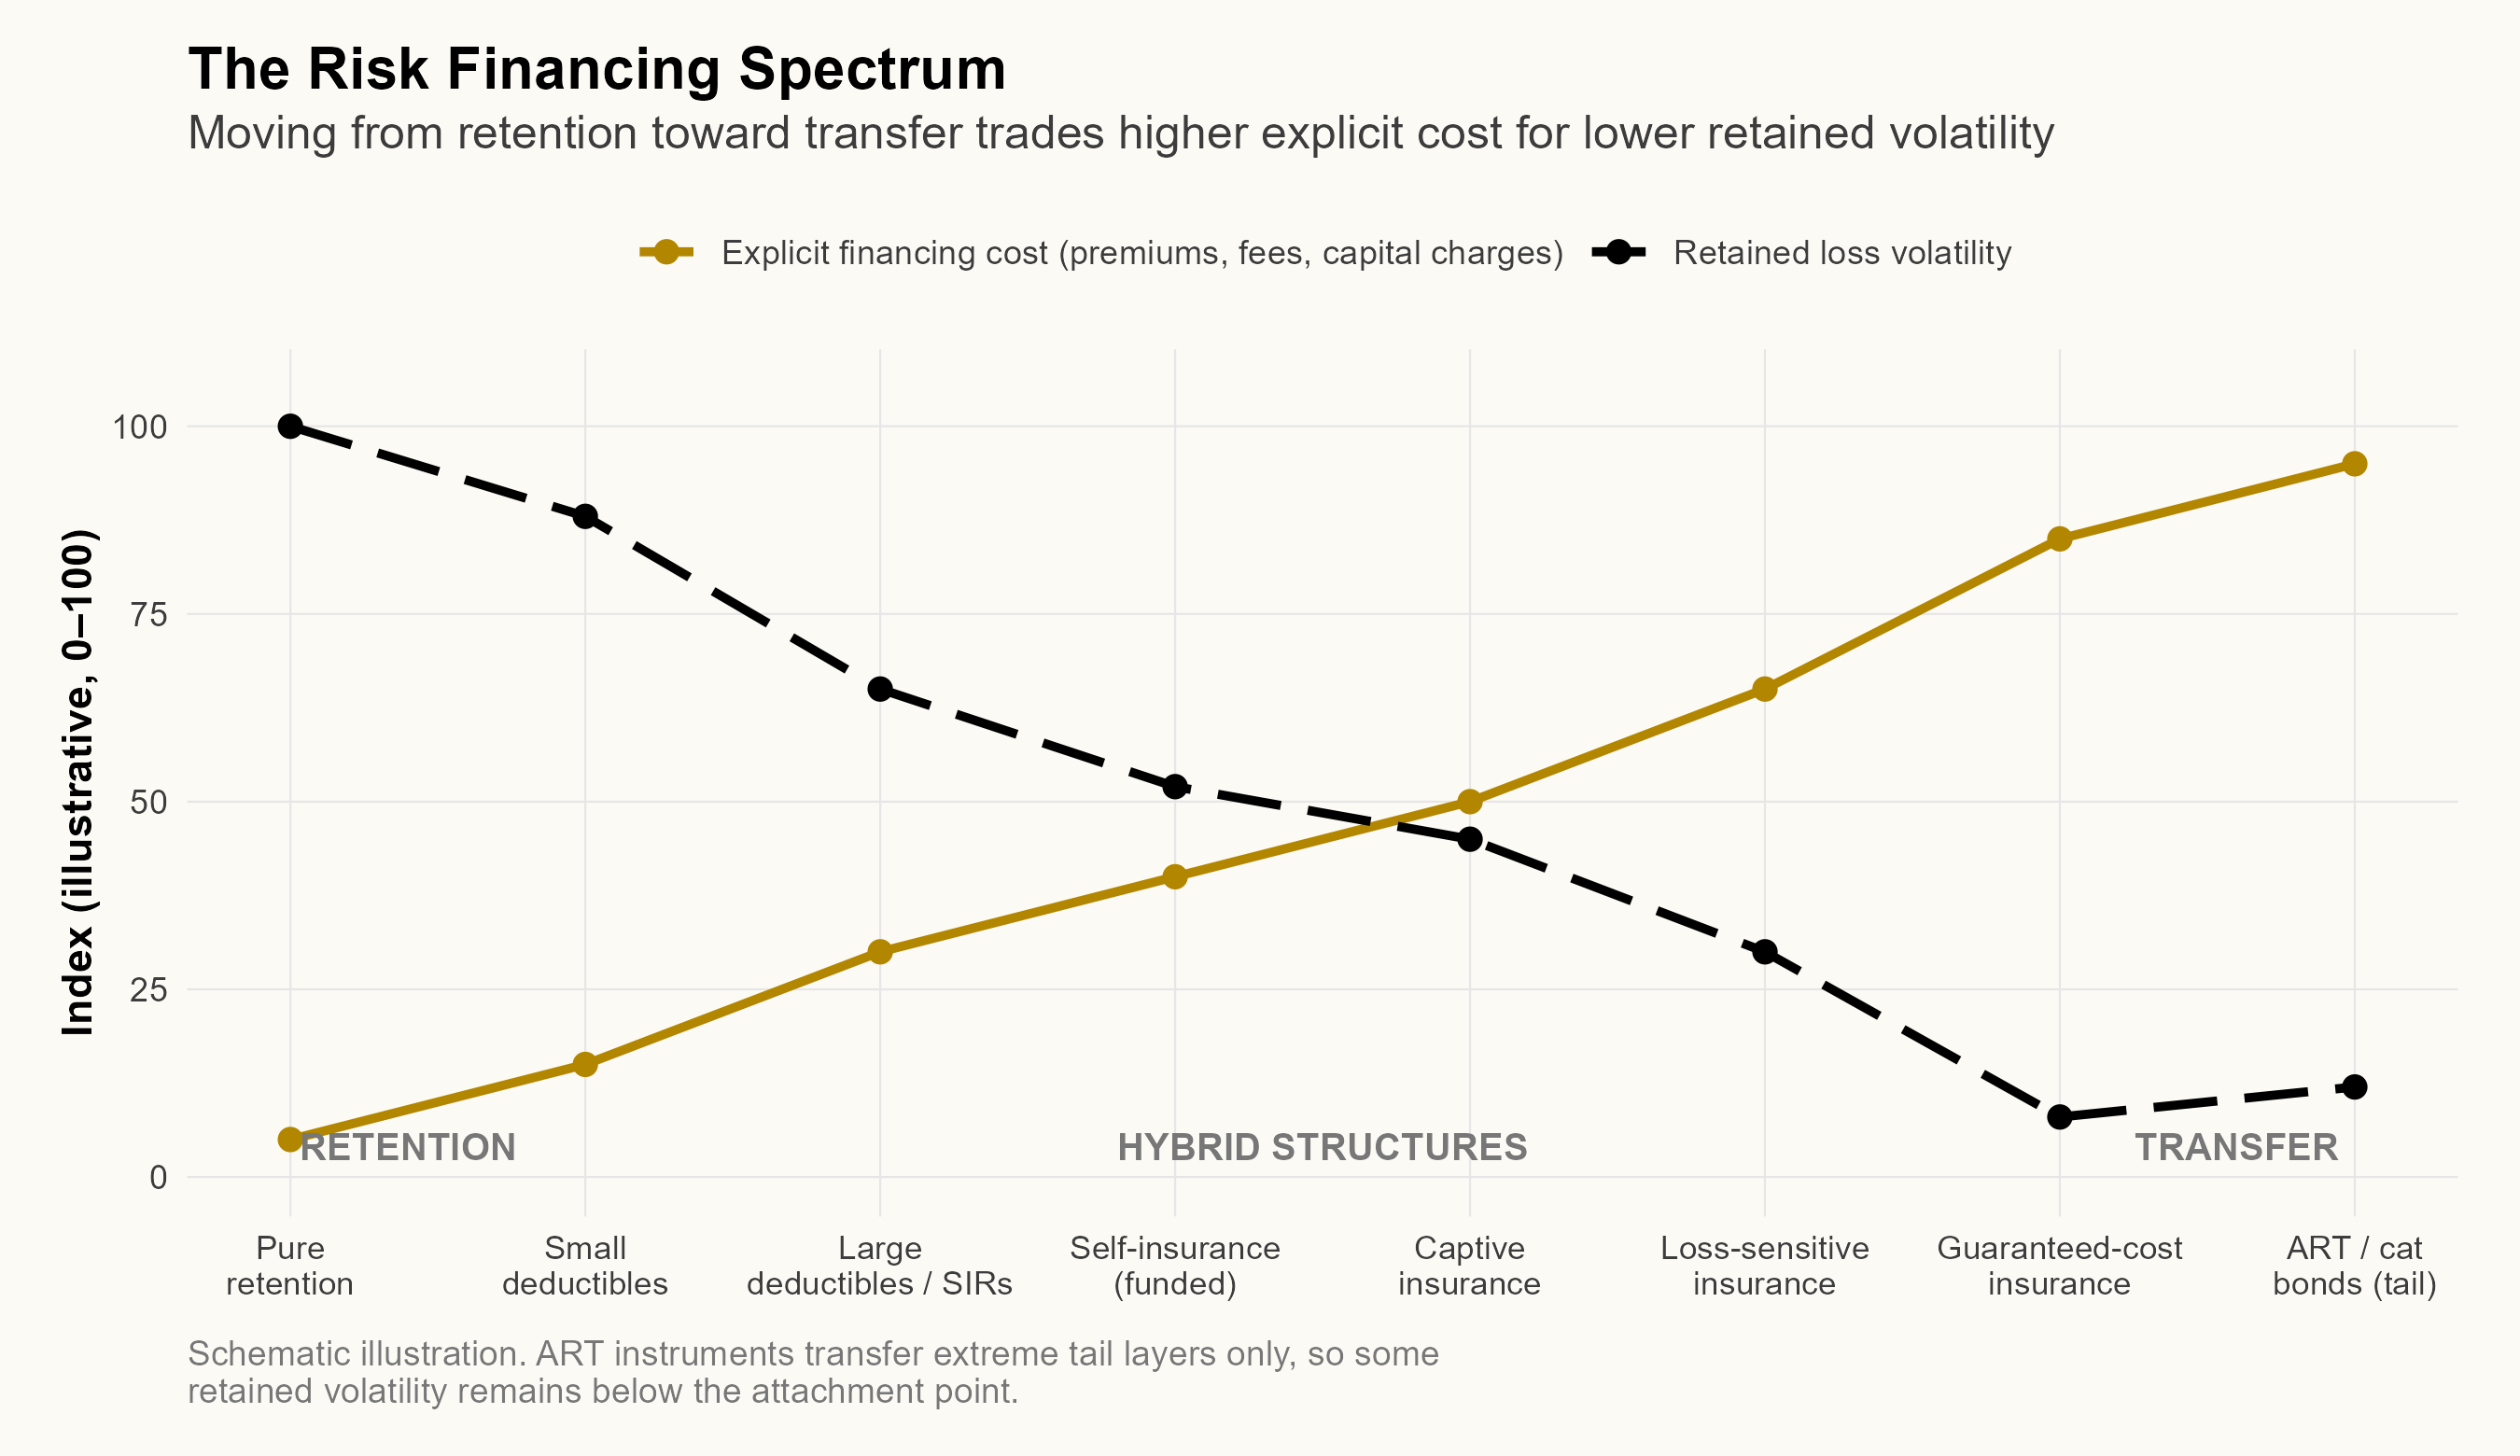
\includegraphics[width=\textwidth]{c8_financing_spectrum.png}
  \caption{The risk financing spectrum. Moving from retention toward transfer
  raises the explicit cost of financing and reduces retained loss volatility.
  ART instruments sit at the high-cost end but transfer only extreme tail
  layers, so some retained volatility remains below the attachment point.}
  \label{fig:spectrum}
  \figurenote{Schematic illustration; index values are illustrative rather
  than data. Generated by \texttt{rscripts/chapter8/c8\_financing\_spectrum.r}.}
\end{figure}

\textbf{Pure retention.}\index{risk retention} The organization absorbs all losses internally,
paying claims as they occur from operating cash flow or dedicated reserves.
Explicit cost is minimal (no premiums), volatility is maximal, and the
organization keeps complete control over claims.

\textbf{Small deductibles.} Most commercial policies include
deductibles\index{deductibles}---the amount the insured pays before insurance responds. Small
deductibles (\$10,000--\$50,000) reduce premiums modestly (5--15\%) while
eliminating nuisance claims that cost more to administer than they are worth.

\textbf{Large deductibles and SIRs.} Organizations with strong balance sheets
often choose retentions of \$250,000 to \$1 million or more per occurrence,
cutting premiums 30--50\% while retaining frequency exposure and transferring
severity. A \emph{self-insured retention (SIR)}\index{self-insured retention (SIR)} functions like a large
deductible with a legal distinction: under an SIR the insured pays claimants
directly before insurance attaches, whereas a deductible is typically
advanced by the insurer and reimbursed by the insured. SIRs are common in
liability lines, where direct payment reduces administrative friction.

\textbf{Funded self-insurance.} A formal program of retention backed by
actuarially determined reserves, professional claims administration, and
aggregate stop-loss protection (Section~\ref{sec:self-insurance}).

\textbf{Captive insurance.} The organization establishes its own licensed
insurance subsidiary to formally retain and manage risk while gaining tax,
regulatory, and reinsurance-access advantages (Section~\ref{sec:captives}).

\textbf{Loss-sensitive insurance.} Retrospectively rated programs and
dividend plans link the final premium to actual loss experience, blending
retention and transfer within a single policy
(Section~\ref{subsec:pricing-mechanics}).

\textbf{Guaranteed-cost insurance.} Fixed-premium coverage with no
loss-sensitive features provides maximum budget certainty: the insured knows
its exact insurance cost for the period regardless of losses, and pays the
highest expense load for the privilege.

\textbf{Alternative risk transfer.} Catastrophe bonds, sidecars, industry
loss warranties, and finite structures occupy the far end of the spectrum.
Note the wrinkle visible in Figure~\ref{fig:spectrum}: ART instruments
typically transfer only extreme tail layers, so some retained volatility
remains below the attachment point even as explicit cost peaks.

\subsection{The Cost--Volatility Tradeoff}
\label{subsec:cost-volatility}

Moving rightward along the spectrum costs more and retains less volatility.
The tradeoff\index{cost-volatility tradeoff} reflects an economic reality rather than an arbitrary pricing
convention: volatility reduction is a service, and the insurers and investors
who provide it require compensation for bearing risk and for their costs of
doing business.

Insurance premiums exceed expected losses by the expense load\index{expense load}:

\[
\text{Premium} = \text{Expected Loss} \times (1 + \text{Expense Load})
\]

where the load covers acquisition costs (agent and broker commissions,
marketing, underwriting---roughly 10--15\% of premium), administrative
expenses (claims adjustment, policy servicing, overhead---another 10--15\%),
and underwriting profit and contingencies (5--10\%) (Insurance Information
Institute, 2023). Expressed as a markup over expected losses rather than a
share of premium, typical commercial property-casualty loads run 25--40\%.

A concrete example. An organization with \$1 million in expected annual
property losses faces a premium of roughly \$1.4 million for ground-up
coverage---a 40\% markup, or \$400,000 of expense load. Suppose instead it
retains the first \$500,000 per occurrence through a large deductible.
Expected retained losses are \$600,000 (the frequent small claims account for
most expected loss), and the premium for excess coverage falls to
\$600,000---covering \$400,000 of expected transferred losses at a steeper
50\% markup, because excess layers carry proportionally higher loads. Total
cost falls from \$1.4 million to \$1.2 million: the organization saves
\$200,000 by no longer paying an expense load on losses it could finance
itself, and accepts the volatility of the retained layer in exchange.

The optimization logic generalizes. Retain predictable, high-frequency losses
where the law of large numbers makes outcomes nearly certain and the expense
load buys little; transfer unpredictable, low-frequency/high-severity
exposures where volatility reduction per premium dollar is greatest; and cap
the maximum retained loss so the program respects risk appetite.
Section~\ref{sec:tcor} formalizes this intuition as TCOR optimization.

\subsection{Factors Influencing Position on the Spectrum}

Organizations settle at different points on the spectrum for identifiable
reasons.

\textbf{Financial strength.} Large, profitable corporations with substantial
reserves and diversified operations gravitate toward retention; they can
absorb bad years without distress. Small businesses with limited capital must
transfer risks that could threaten solvency.

\textbf{Risk tolerance and culture.}\index{risk tolerance} From Chapter~5,
the risk appetite\index{risk appetite} framework constrains financing structure directly.
Conservative boards may mandate low retentions and comprehensive insurance
despite the higher cost, prioritizing earnings stability. Boards comfortable
with volatility may retain aggressively to minimize premium spend.

\textbf{Loss predictability.} Stable, high-frequency loss patterns support
confident retention---workers' compensation for a large employer with mature
safety programs is the standard example. Catastrophic exposures with low
frequency and devastating severity warrant transfer despite expensive
pricing; this is precisely where OLC landed on earthquake.

\textbf{Access to capital markets.} Publicly traded corporations with ready
access to equity and debt can finance retained losses through normal treasury
operations. Private companies, or firms near covenant limits, lack that
flexibility---for them insurance functions as contingent capital.

\textbf{Regulatory and contractual requirements.} States require proof of
financial responsibility for workers' compensation and auto liability;
lenders and counterparties routinely mandate insurance. These requirements
constrain retention regardless of what economic optimization would suggest.

\textbf{Tax considerations.} Premiums paid to qualified insurers are
immediately deductible; self-insured losses may face timing disadvantages.
Captives offer planning opportunities under anti-abuse scrutiny
(Section~\ref{subsec:captive-tax}).

\textbf{Management expertise and systems.} Sophisticated retention requires
claims systems, actuarial capability, and experienced staff. Organizations
without that infrastructure may rationally pay higher premiums for
administrative simplicity.

% =======================================================================
\section{Retention versus Transfer: The Core Decision}
\label{sec:retention-transfer}

\subsection{The Fundamental Cost Comparison}
\label{subsec:cost-comparison}

For any given exposure, the organization compares total expected costs\index{risk retention!versus transfer}:

\begin{align*}
\text{Total Cost of Retention} ={}& E[\text{Retained Losses}]
+ \text{Cost of Capital Held Against Losses} \\
&+ \text{Administrative Costs}
\end{align*}

\begin{align*}
\text{Total Cost of Transfer} ={}& \text{Insurance Premiums}
+ \text{Residual Retained Losses} \\
&+ \text{Brokerage and Fees}
\end{align*}

The decision minimizes total expected cost subject to risk appetite
constraints.

\textbf{Cost of retention.} Retaining risk requires capital held against
potential losses, and that capital has an opportunity cost at the firm's cost
of capital\index{cost of capital} \(k\). Required reserves typically equal expected losses plus a
safety margin tied to the loss distribution from
Chapter~4---for instance, reserves at the 95th
percentile:

\[
\text{Required Reserves} = E[\text{Losses}]
+ \big(\text{VaR}_{0.95} - E[\text{Losses}]\big) = \text{VaR}_{0.95}
\]

Suppose an organization expects \$2 million in annual losses with VaR(95\%)
of \$3.5 million, and its cost of capital is 10\%. The annual opportunity
cost of holding reserves at VaR is \(\$3.5\text{M} \times 0.10 =
\$350{,}000\). Adding expected losses of \$2 million and administrative costs
(claims handling, safety programs) of \$200,000:

\[
\text{Total Annual Cost of Retention}
= \$2{,}000{,}000 + \$350{,}000 + \$200{,}000 = \$2{,}550{,}000
\]

\textbf{Cost of transfer.} Full insurance for the same exposure, at a 35\%
expense load, costs \(\$2\text{M} \times 1.35 = \$2.7\) million in premium.
Adding broker fees of 5\% of premium (\$135,000) and roughly \$100,000 of
expected losses retained within small per-claim deductibles:

\[
\text{Total Annual Cost of Transfer}
= \$2{,}700{,}000 + \$135{,}000 + \$100{,}000 = \$2{,}935{,}000
\]

\textbf{Decision.} Retention costs \$2.55 million against \$2.935 million for
transfer---a saving of \$385,000 annually, about 13\%. But retention exposes
the organization to outcomes as bad as \$3.5 million (and worse, beyond the
95th percentile). If the board's risk appetite caps acceptable annual loss
volatility at \$3 million, retention is infeasible regardless of its expected
savings. The appetite constraint, not the cost comparison, is binding---a
pattern that recurs throughout this chapter.

\subsection{The Optimal Retention Level}
\label{subsec:optimal-retention}

Rather than choosing pure retention or pure transfer, most organizations
select a retention level\index{optimal retention level}---a deductible or SIR---that balances premium
savings against capital costs and appetite limits. Formally:

\[
\min_{R} \; \text{TCOR}(R) = E[L(R)] + k \cdot C(R) + P(R) + \text{Admin}(R)
\quad \text{s.t.} \quad \text{VaR}_{0.95}(R) \le \text{Appetite Limit}
\]

where \(R\) is the retention level, \(E[L(R)]\) the expected retained losses
at retention \(R\), \(C(R)\) the capital required to support that retention,
\(k\) the cost of capital, \(P(R)\) the premium for excess coverage above
\(R\), and \(\text{Admin}(R)\) administrative costs.

The comparative statics are intuitive. As \(R\) rises, expected retained
losses and required capital rise while premium falls; retained VaR rises
until it hits the appetite boundary. The optimum \(R^{*}\) is where marginal
premium savings stop covering the marginal cost of retained losses and
capital---or where the appetite constraint binds, whichever comes first.

\textbf{Worked example.} An organization faces property losses with expected
annual loss of \$1.5 million and a loss standard deviation of \$900,000. Its
cost of capital is 12\%, the insurer's expense load is 35\%, capital is held
at 150\% of expected retained losses, and the board's appetite limit is
VaR(95\%) \(\le\) \$4 million. Table~\ref{tab:retention-levels} evaluates
three candidate retentions.

\begin{ermtable}{Retention alternatives compared (\$000s)}[tab:retention-levels]
\begin{tabular}{@{}lrrrrrrr@{}}
\toprule
\textbf{Retention} & \textbf{Retained} & \textbf{Capital} &
\textbf{Cap.\ cost} & \textbf{Transferred} & \textbf{Premium} &
\textbf{Total} & \textbf{VaR(95\%)} \\
 & \textbf{loss} & \textbf{(150\%)} & \textbf{@12\%} &
\textbf{loss} & \textbf{@1.35\(\times\)} & & \\
\midrule
\$0 (full ins.) & 0 & 0 & 0 & 1{,}500 & 2{,}025 & 2{,}025 & \(\approx 0\) \\
\$500K & 400 & 600 & 72 & 1{,}100 & 1{,}485 & 1{,}957 & 2{,}800 \\
\$1M & 700 & 1{,}050 & 126 & 800 & 1{,}080 & 1{,}906 & 3{,}500 \\
\bottomrule
\end{tabular}
\tablenote{Premiums equal 1.35 times expected transferred losses; capital is
held at 150\% of expected retained losses with a 12\% opportunity cost.}
\end{ermtable}

Full insurance costs \$2,025K and eliminates volatility. The \$500K retention
saves \$68K annually (3.4\%) with retained VaR comfortably inside the limit.
The \$1M retention saves \$119K (5.9\%) and still respects the \$4M appetite.
The optimal retention is \$1M---the highest candidate whose VaR remains
inside appetite. Note what drives the result: every dollar of expected loss
moved from the transferred to the retained column saves its 35-cent expense
load but costs 18 cents of capital charge (150\% \(\times\) 12\%), so
retention wins on expected cost until the appetite constraint stops it.

\subsection{Decision Rules and Heuristics}

Quantitative optimization is the right framework, but practitioners lean on a
handful of rules that capture most of its content.

\textbf{Rule 1: Retain high-frequency, low-severity risks.} Frequent losses
with predictable severity are prime retention candidates---the law of large
numbers makes annual outcomes nearly certain, so the expense load buys
nothing. Fleet physical damage for a 500-vehicle company; employee health
claims for a large employer.

\textbf{Rule 2: Transfer low-frequency, high-severity risks.} Catastrophic
exposures that could threaten viability warrant transfer despite expensive
pricing. Product liability for a pharmaceutical manufacturer; earthquake for
a Tokyo Bay theme park; cyber breach liability for a retailer holding payment
card data.

\textbf{Rule 3: Cap retention by financial capacity.} A conservative rule of
thumb: maximum aggregate annual retention should not exceed 5--10\% of net
worth or 15--20\% of pre-tax earnings, so a bad year does not become a
distress event.

\textbf{Rule 4: Transfer non-core risks, retain core competencies.} Transfer
risks where insurers hold informational and claims-handling advantages
(directors and officers liability for an operating company). Retain risks
central to operations---product quality, employee safety---where the
organization controls outcomes better than any insurer could.

\textbf{Rule 5: Evaluate correlation in aggregate.} From
Chapter~6, retention decisions made line by line
ignore portfolio effects. Retaining several uncorrelated exposures is safer
than the line-by-line view suggests; retaining correlated ones is more
dangerous. Section~\ref{subsec:multiline} quantifies this.

% =======================================================================
\section{Traditional Risk Financing: Commercial Insurance}
\label{sec:commercial-insurance}

\subsection{The Insurance Value Proposition}

Insurance\index{commercial insurance} performs three economic functions that justify paying an expense
load rather than retaining.

\textbf{Risk pooling and diversification.}\index{risk pooling}\index{diversification} Insurers pool thousands or
millions of largely independent exposures, achieving diversification no
single insured can replicate. The law of large numbers\index{law of large numbers} makes the insurer's
aggregate outcome predictable even though each insured's outcome is not
(Rejda \& McNamara, 2017).

\textbf{Claims expertise.} Professional insurers bring specialized capability
in claims investigation, defense, and settlement that reduces total claim
cost: medical cost containment in workers' compensation, litigation
management in liability, negotiated repair networks in property. For complex
claims these savings can exceed the insurer's entire administrative fee
(Harrington \& Niehaus, 2004).

\textbf{Contingent capital.}\index{contingent capital} The insurer's promise to pay is pre-arranged
financing activated by loss events. For organizations with limited capital
market access or binding covenants, this contingent capital has value beyond
the loss payment itself (Froot et al., 1993)---the same economic function OLC
bought from bond investors, purchased instead from an insurer's balance
sheet.

\subsection{Major Commercial Insurance Lines}
\label{subsec:lines}

\textbf{Property insurance}\index{property insurance} covers direct physical damage to buildings,
equipment, and inventory from covered perils. Standard commercial forms use
``special form'' (all-risks) coverage---protection against everything except
specific exclusions, commonly flood, earthquake (both separately insurable),
war, and nuclear hazard (Insurance Services Office, 2012). Typical structures
include per-occurrence deductibles from \$5,000 to \$1 million or more,
limits set at insured values or blanket limits across locations, coinsurance
clauses requiring insurance to at least 80--90\% of value, and optional
business interruption coverage for lost income during restoration. Recall
from Chapter~3 that business interruption is an
operational/hazard exposure; the insurance that finances it rides on the
property form.

\textbf{Commercial general liability (CGL)}\index{commercial general liability (CGL)} provides third-party coverage for
bodily injury and property damage arising from premises, operations, and
products. CGL is written on an \emph{occurrence} basis\index{occurrence versus claims-made coverage}: coverage attaches
based on when the injury occurred, regardless of when the claim is filed,
creating long-tail exposure in which claims surface years after policy
expiration (Harrington \& Niehaus, 2004). Typical structures: per-occurrence
limits of \$1--5 million, general aggregate limits of \$2--10 million,
separate products/completed-operations aggregates, and defense costs paid in
addition to limits.

\textbf{Workers' compensation}\index{workers' compensation}, mandatory in most states, pays statutory
medical and wage-replacement benefits to injured employees while shielding
employers from tort liability under the exclusive remedy doctrine\index{exclusive remedy doctrine}. Because
benefits are prescribed by statute, loss patterns are comparatively
predictable---which is why workers' compensation is the most common line for
large-deductible programs and self-insurance (National Academy of Social
Insurance, 2021). Premiums adjust to the employer's own loss history through
the experience modification rate (EMR)\index{Experience Modification Rate (EMR)} introduced in
Chapter~7.

\textbf{Professional liability (errors and omissions)}\index{professional liability insurance} covers economic
damages from professional mistakes or failure to deliver promised
services---architects, engineers, accountants, consultants, technology
providers. Unlike occurrence-based CGL, professional liability is written on
a \emph{claims-made} basis\index{occurrence versus claims-made coverage}, covering only claims first made during the policy
period. The distinction matters when switching insurers or winding down
operations, when ``tail'' coverage must be purchased to cover claims not yet
reported.

\subsection{Insurance Pricing Mechanics}
\label{subsec:pricing-mechanics}

Actuaries build rates from the pure premium\index{pure premium}---expected loss per unit of
exposure:

\[
\text{Loaded Premium} = \text{Pure Premium}
\times (1 + \text{Expense Load})
\times (1 + \text{Profit and Contingency Margin})
\]

For property, the exposure base is \$100 of insured value; the pure premium
is historical loss cost per \$100, trended and adjusted for territory,
construction, protection class, and occupancy. A manufacturer insuring a \$10
million building might face a pure premium of \$0.25 per \$100 loaded to
\$0.34, for a total premium of \$34,000. For liability lines the exposure
base varies by classification---payroll for workers' compensation, sales for
products liability---and loads run higher (35--45\%) because of defense costs
and long claim durations.

Beyond fixed-price (``guaranteed cost'') policies, insurers offer
loss-sensitive structures that blend retention and transfer.

\textbf{Experience rating}\index{experience rating} adjusts premiums based on the insured's own
multi-year loss history. Workers' compensation experience rating through the
EMR is mandatory above a premium threshold; other lines offer credits and
debits at the underwriter's discretion.

\textbf{Retrospective rating}\index{retrospective rating} sets the final premium after the policy period
based on actual losses:

\[
\text{Retro Premium} = (\text{Basic Premium} + \text{Converted Losses})
\times \text{Tax Multiplier}
\]

subject to a minimum premium (often 60--70\% of standard) and a maximum
(often 125--140\%). The basic premium covers insurer overhead and profit;
converted losses are actual losses grossed up by a loss conversion factor
(typically 1.10--1.15) for claims-handling expense. The insured benefits
directly from good experience and is protected from catastrophic experience
by the maximum.

\textbf{Large-deductible and SIR programs}
(Section~\ref{subsec:optimal-retention}) reduce premiums to the cost of
excess coverage plus service fees.

\textbf{Dividend plans} return a portion of premium if losses run below
target thresholds---a profit-sharing arrangement common in workers'
compensation, where dividends of 20--40\% of premium are achievable for
excellent experience.

\subsection{Insurance Market Cycles: Hard and Soft Markets}
\label{subsec:market-cycles}

Insurance pricing is cyclical\index{insurance market cycle}, driven by industry capital and competitive
dynamics. In a \textbf{soft market}\index{soft market}, abundant capacity produces aggressive
pricing at or below actuarially indicated rates, broad coverage terms, and
readily available limits; insurer combined ratios drift above 100\% with
investment income covering the gap. In a \textbf{hard market}\index{hard market}, capital
impairment---from catastrophes or investment losses---produces rate increases
of 10--50\% or more at renewal, narrowed terms, withdrawn capacity, and
restored underwriting discipline.

Major hardenings followed September 11, 2001, Hurricane Katrina in 2005, and
the 2017--2021 period of heavy catastrophe losses capped by the pandemic. The
strategic implication for insureds: anticipate the cycle rather than chase
it. Organizations that slash retentions when coverage is cheap, then face
unaffordable renewals when the market turns, pay more over the cycle than
those that hold a stable program designed around their own risk-bearing
capacity (Insurance Information Institute, 2023). The market cycle is also a
standing argument for the alternative mechanisms in
Sections~\ref{sec:captives}--\ref{sec:securitization}, which insulate part of
the program from renewal repricing.

% =======================================================================
\section{Self-Insurance and Retention Programs}
\label{sec:self-insurance}

\subsection{Self-Insurance Fundamentals}

\textbf{Self-insurance}\index{self-insurance} is the deliberate, structured decision to retain risk
and pay losses from organizational resources. The word \emph{structured}
distinguishes it from ``going bare''---operating without coverage because
insurance seems expensive. A true self-insurance program incorporates
actuarial funding (reserves accumulated against projected losses), formal
claims administration, integrated safety and loss control, aggregate
protection capping extreme outcomes, and compliance with state financial
responsibility requirements.\footnote{Regulatory requirements for
self-insurance vary substantially by state and coverage type. Organizations
considering self-insurance should consult qualified advisors in every
jurisdiction where they operate.}

\subsection{When Self-Insurance Makes Economic Sense}

Five conditions favor self-insurance, and most successful programs satisfy
all of them.

\textbf{Scale and predictability.} Enough exposure units---employees,
vehicles, locations---that the law of large numbers operates internally.
Common benchmarks: 500+ employees for workers' compensation; 250+ vehicles
for auto liability.

\textbf{Financial capacity.} Balance sheet strength to absorb adverse years.
Rule of thumb: required reserves (expected losses plus 1.5--2.0 standard
deviations) should not exceed 15--20\% of net worth.

\textbf{Superior risk management.} Organizations that consistently outperform
industry loss averages subsidize weaker risks when they buy insurance priced
to the average. Self-insurance lets them keep the difference---the same logic
that justified Mercer Tool \& Stamping's loss control investment in
Chapter~7 carries over to financing.

\textbf{Expense load savings exceed administration costs.} Self-insurance
eliminates the insurer's 25--40\% load but adds internal or third-party
administration costs of roughly 5--15\% of losses. The net must be positive.

\textbf{Cash flow value.} Retaining cash until losses are paid, rather than
paying premiums in advance, benefits organizations whose investment
opportunities exceed the risk-free rate.

\subsection{Self-Insurance Program Structure}

\textbf{Funding mechanisms.} A \emph{pre-funded reserve account} accumulates
contributions equal to expected losses plus a margin, reaching steady state
at expected outstanding liabilities; for tax purposes, contributions are not
deductible---only paid losses are (26 U.S.C. \S~162). \emph{Pay-as-you-go}
funding pays claims from operating cash as they come due, maximizing cash
availability at the cost of volatile cash flows. To satisfy state security
requirements without tying up cash, organizations post \emph{letters of
credit} (bank fees of 1--3\% annually) or \emph{surety bonds} (2--5\% of face
amount).

\textbf{Claims administration.} Self-insureds must handle claims
professionally or pay for sloppiness in settlements, litigation, and
regulatory penalties. Three models: \emph{internal administration} (dedicated
staff---economic only for very large programs, roughly 5,000+ employees or
\$10M+ annual claims); \emph{third-party administrators (TPAs)}\index{third-party administrator (TPA)}, independent
firms that investigate, negotiate, and pay claims for fees of \$150--\$400
per claim or 8--12\% of incurred losses; and \emph{fronting arrangements}\index{fronting arrangement}, in
which a licensed insurer issues the policy and administers claims while the
insured retains the economic risk through deductible reimbursement
obligations.

\textbf{Aggregate stop-loss protection.}\index{aggregate stop-loss} Pure self-insurance leaves the
program exposed to a bad cluster of claims in a single year. Aggregate
stop-loss insurance caps annual retained losses at an attachment point,
typically 125--150\% of expected losses. An organization expecting \$3
million of workers' compensation losses might attach aggregate coverage at
130\%---\$3.9 million. If actual losses reach \$5 million, the stop-loss
insurer pays the \$1.1 million above the attachment. Premiums for the
aggregate layer typically run 5--15\% of the covered layer.

\subsection{Regulatory Requirements}

States regulate self-insurance to protect claimants---particularly injured
workers---from employers who retain risk without the capacity to pay.
Workers' compensation self-insurance typically requires state approval with
minimum net worth thresholds (\$1--25 million depending on state), audited
financials and actuarial certification of reserves, security deposits (cash,
letters of credit, or surety bonds scaled to payroll and loss history), proof
of specific and aggregate excess coverage, demonstrated claims administration
capability, and annual fees and assessments.

First-party property self-insurance is generally unregulated---the
organization bears the consequences of its own choices. Liability
self-insurance faces restrictions wherever third parties could be left
uncompensated: auto liability financial responsibility laws, environmental
bonding requirements for hazardous operations, and professional licensing
board requirements.

% =======================================================================
\section{Captive Insurance Companies}
\label{sec:captives}

\subsection{The Captive Concept}

A \textbf{captive insurance company}\index{captive insurance} is a licensed insurer owned and
controlled by its insureds, formed primarily to cover the risks of its parent
organization. A captive formalizes retention inside an insurance company
structure---with capital requirements, regulatory oversight, and professional
management---and in exchange gains the legal and economic standing of an
insurer. Roughly 7,000 captives operate worldwide, with U.S. corporations
accounting for about 40\% of formations (Captive Insurance Companies
Association, 2022).\footnote{Captive formation and operation require
compliance with domicile insurance regulation, federal and state tax law, and
parent-company accounting standards. Professional guidance from captive
managers, actuaries, tax counsel, and auditors is essential, and its cost
belongs in the captive feasibility analysis.}

Five defining characteristics: ownership by insureds rather than outside
shareholders; primary business of insuring parent risks; licensure and
regulation in a domicile jurisdiction; minimum capital and surplus
requirements; and professional underwriting, claims, actuarial, and
investment management.

The economic rationale parallels the value channels of
Section~\ref{subsec:value-channels}, applied through an insurance subsidiary.
The captive eliminates the commercial insurer's profit margin and overhead,
paying only incremental administration, regulatory, and reinsurance costs.
Premium paid to the captive accumulates as captive surplus and earns
investment income for the parent rather than for a commercial insurer---the
``float'' stays home. Premiums may be tax-deductible while the captive's
income enjoys favorable insurance company taxation
(Section~\ref{subsec:captive-tax}). The captive can write coverage that
commercial markets price punitively or refuse outright---terrorism, product
recall, brand protection, cyber---on terms the parent designs. And the
captive buys reinsurance directly at wholesale, skipping a layer of
intermediary loading.

\subsection{Types of Captive Structures}

\textbf{Single-parent (pure) captive.}\index{captive insurance!structures} Owned by one operating company to
insure its own risks; maximum control, but the parent funds all capital and
operating costs. Typical minimum capital: \$250,000--\$500,000 plus loss
reserves; annual operating costs \$75,000--\$200,000 for small captives and
\$250,000+ for sophisticated ones.

\textbf{Group captive.}\index{group captive} Owned by multiple unrelated organizations---usually
in the same industry---pooling homogeneous risks and sharing fixed costs.
Hospital systems pooling malpractice; contractors pooling workers'
compensation.

\textbf{Association captive.} Sponsored by a trade association for its
members; functionally a group captive or mutual with association governance.
Municipal workers' compensation pools and design-professional liability
captives are common examples.

\textbf{Protected cell company (PCC) / segregated portfolio company (SPC).}\index{protected cell company (PCC)} A
single licensed entity containing legally segregated ``cells,'' each with its
own assets and liabilities. Cells share infrastructure---cutting formation
cost---without sharing solvency. Cell rental runs \$25,000--\$75,000
annually, far below dedicated captive costs, making cells the entry point for
mid-sized firms.

\textbf{Rent-a-captive.} Participants rent underwriting capacity from an
existing captive---fastest market entry, least control.

\textbf{Agency captive.} Owned by an insurance agency to write its clients'
business. The structure creates obvious conflicts of interest (the broker
profits from placing business in its own captive) and draws regulatory
scrutiny.

\subsection{Captive Domicile Selection}

A captive must be licensed somewhere, and domiciles compete for formations on
regulation, tax, and cost\index{captive insurance!domicile selection}. \textbf{Vermont} is the oldest and largest U.S.
domicile (800+ captives), with a sophisticated regulator, deep
service-provider infrastructure, and a premium tax of 0.4\% capped at
\$200,000 for most captives. \textbf{Delaware} (roughly 400 captives) offers
no state premium tax and familiar corporate law. South Carolina, North
Carolina, Tennessee, and Utah market actively to home-state corporations.
Offshore, \textbf{Bermuda} (700+ captives) offers no corporate income tax,
respected regulation, and direct access to the world's largest reinsurance
market, at operating costs of \$150,000--\$300,000 annually and with U.S.
controlled-foreign-corporation tax complications; the \textbf{Cayman Islands}
is comparable with particularly flexible segregated portfolio legislation;
\textbf{Luxembourg, Ireland, and Malta} give EU passporting rights important
to multinationals with European operations.

Selection turns on tax treatment, regulatory quality, operating cost,
reinsurance access, proximity to the parent, legal infrastructure, and
political stability. In practice the choice is usually between the parent's
home-state domicile (administrative convenience, political goodwill) and a
major established domicile (depth of expertise).

\subsection{Tax Considerations}
\label{subsec:captive-tax}

Tax treatment can make or break captive economics\index{captive insurance!tax considerations}, and it attracts
correspondingly aggressive structuring and correspondingly aggressive
enforcement.

\textbf{Premium deductibility.} For premiums paid to a captive to be
deductible under 26 U.S.C. \S~162(a), the arrangement must be
\emph{insurance} in the sense of \emph{Helvering v.\ Le Gierse}\index{Helvering v. Le Gierse}, 312 U.S. 531
(1941) and its progeny, which requires both \textbf{risk transfer} (genuine
shifting of economic loss to the captive) and \textbf{risk distribution}\index{risk distribution}
(pooling across enough exposures for the law of large numbers to operate).
Single-parent captives insuring only the parent have historically struggled
with risk distribution. Accepted strategies include writing substantial
unrelated third-party business (often 30\%+ of premium), participating in
group structures or reinsurance pools, and insuring numerous operating
subsidiaries---though the IRS views brother-sister arrangements skeptically.

\textbf{The \S~831(b) election.}\index{831(b) election} ``Micro-captives'' with annual premiums at
or below the inflation-indexed limit (\$2.85 million for 2025) may elect
taxation on investment income only, paying no federal income tax on
underwriting income, provided diversification requirements are met (no more
than 20\% of premium from one insured). The election is legitimate for
genuinely operating small captives---and has been heavily abused by promoters
selling captives as estate-planning and tax shelters with token risk
transfer. The IRS designated certain micro-captive transactions as reportable
``listed transactions'' in Notice 2016-66; after that notice was set aside on
procedural grounds in litigation, the IRS finalized regulations in 2024
re-designating abusive micro-captive structures as listed transactions or
transactions of interest.\footnote{Genuine risk transfer, arm's-length
pricing, and adequate capitalization remain the touchstones; the procedural
litigation changed the disclosure mechanics, not the substantive
requirements.} The substance requirements are unchanged: real risk transfer,
arm's-length pricing, adequate capitalization, and a business purpose beyond
tax savings.

\textbf{Controlled foreign corporation rules.}\index{controlled foreign corporation (CFC) rules} Offshore captives owned by
U.S. parents are typically CFCs, and Subpart F (26 U.S.C. \S\S~951--965) can
pull insurance income into current U.S. taxation even if undistributed.
Exceptions exist for qualifying insurance income, but the analysis is
intricate and domicile-dependent---one reason the U.S. domiciles have grown
at the offshore centers' expense.

% =======================================================================
\section{Alternative Risk Transfer Instruments}
\label{sec:art}

\subsection{The ART Rationale}

\textbf{Alternative risk transfer (ART)}\index{alternative risk transfer (ART)} covers the non-traditional
mechanisms that blend insurance and capital market techniques, often
packaging multiple risks or multiple years into a single transaction. ART
emerged in the 1990s from a convergence of pressures: capacity crises that
made conventional coverage unavailable or unaffordable; corporate
dissatisfaction with one-year, one-line insurance pricing; the recognition
that global capital markets (measured in the hundreds of trillions of
dollars) dwarf the insurance industry's risk-bearing capacity (single-digit
trillions); and quantitative modeling advances that made bespoke structures
priceable. OLC's Midori bond is the cleanest illustration of the underlying
idea---when the risk is well-modeled and the traditional market is expensive,
go directly to investors.

\subsection{Finite Risk Insurance and Reinsurance}
\label{subsec:finite}

\textbf{Finite risk}\index{finite risk insurance} products cap the insurer's maximum loss at a modest
multiple of premium---typically 110--125\%---and explicitly price the time
value of money. Where traditional insurance transfers underwriting risk,
finite structures primarily transfer \emph{timing} risk, smoothing losses
over multi-year horizons.

Key features: premiums set well above expected losses (often 150--200\%),
with the excess accumulating in an \textbf{experience account}\index{experience account} that earns
interest at contractual rates; multi-year terms of 3--10 years; and
profit-sharing at expiry---favorable experience returns the account balance
to the cedent, adverse experience requires additional premium up to a cap,
and only losses beyond the cap land on the insurer.

\textbf{Example structure.} Calloway Industries\index{Calloway Industries} purchases five-year finite
reinsurance for product liability: annual premium \$2 million (\$10 million
total), expected losses \$6 million over the term, maximum insurer payout
\$12 million (120\% of premium), and a 4\% annual interest credit. Each year
the experience account grows by premium plus interest and is drawn down by
paid losses. At expiry, a positive balance is refunded; a deficit up to \$2
million is repaid by Calloway; anything beyond that cap is the reinsurer's
loss.

Finite risk serves loss smoothing (converting volatile annual outcomes into a
predictable multi-year cost---attractive to public companies managing
earnings guidance), structured funding of long-tail reserves, and regulatory
capital relief for insurers and banks.

The accounting deserves the caution it has earned\index{finite risk insurance!accounting issues}. To qualify for insurance
accounting, a finite contract must transfer genuine risk---both underwriting
and timing risk---under FASB ASC 944; structures that fail the test are
deposits, not insurance. Finite transactions were central to accounting
scandals at AIG and Gen Re in the early 2000s, where contracts with
negligible risk transfer were booked as reinsurance to dress up reserves.
Regulators have scrutinized the product line closely ever since.

\subsection{Multi-Trigger and Integrated Risk Programs}

\textbf{Multi-trigger policies}\index{multi-trigger policies} pay only when two or more specified events
occur together, cutting the probability of payout---and the
premium---relative to single-trigger coverage. Lakeshore Power \& Light\index{Lakeshore Power and Light}, a
utility, buys earthquake coverage that pays only if (1) an earthquake of
magnitude 7.0 or greater strikes its service territory \emph{and} (2) its
stock price falls 25\% or more within 30 days. The double trigger prices at
perhaps 40--60\% of conventional earthquake coverage. The logic is the
financial-distress channel from Section~\ref{subsec:value-channels}: the
company needs external capital only when physical damage coincides with
impaired financing capacity. If the earthquake comes and the stock holds,
treasury operations can fund the repairs.

\textbf{Integrated risk programs}\index{integrated risk programs} combine traditionally separate
lines---property, casualty, marine, political risk, business
interruption---into one policy with an aggregate retention and limit.
Meridian Industrial Group\index{Meridian Industrial Group} consolidates five lines into a single \$500 million
program with a \$50 million aggregate deductible across all perils. Because
the covered perils are imperfectly correlated (the
Chapter~6 logic, applied to insurance purchasing),
the integrated program prices 15--25\% below the sum of standalone policies.
Integrated programs suit multinationals with genuinely diversified exposures;
administrative complexity and jurisdictional insurance requirements limit
broader adoption.

\subsection{Risk Retention Groups}

The federal \textbf{Liability Risk Retention Act of 1986}\index{Liability Risk Retention Act} (15 U.S.C.
\S\S~3901--3906) authorizes \textbf{risk retention groups (RRGs)}\index{risk retention group (RRG)}---liability
insurers owned by their policyholder-members---to operate nationwide under a
single state license, preempting other states' licensing requirements (though
not their solvency oversight). The Act responded to the liability crisis of
the mid-1980s, when entire professions faced unavailable or unaffordable
coverage.

RRGs are restricted to liability lines (no property or workers'
compensation), require member ownership and industry homogeneity, and in some
structures impose joint and several liability among members---an arrangement
that concentrates the mind on underwriting discipline. Roughly 240 RRGs
operate today, concentrated in medical malpractice, product liability, and
commercial auto (National Association of Insurance Commissioners, 2023). They
function well for stable, homogeneous member bases; failures have generally
traced to underpricing or under-reserving in the early years, the standard
failure mode of mutual insurance.

% =======================================================================
\section{Risk Securitization: Catastrophe Bonds and Insurance-Linked
Securities}
\label{sec:securitization}

\subsection{The ILS Market}

\textbf{Insurance-linked securities (ILS)}\index{insurance-linked securities (ILS)} are financial instruments whose
payoffs depend on insurance loss events, transferring risk from insurers,
reinsurers, corporations, and governments to capital market investors. From
experimental transactions in the mid-1990s, the ILS market has grown into a
mature asset class exceeding \$100 billion, providing essential capacity for
catastrophic risk (Swiss Re, 2023).\footnote{The ILS market's modern growth
dates to the capacity shortage after Hurricane Andrew (1992) and accelerated
after Hurricane Katrina (2005). Structures, triggers, and covered perils
continue to evolve.}

The economics work for both sides. Sponsors gain access to risk-bearing
capacity that vastly exceeds the reinsurance industry's capital, particularly
for the low-frequency, high-severity perils---hurricane, earthquake,
pandemic---where reinsurance capacity is scarcest and most cyclical.
Investors gain an asset whose returns are driven by hurricanes and
earthquakes rather than by interest rates and corporate earnings: near-zero
correlation with equity and bond markets makes ILS a genuine diversifier even
at moderate expected returns (Cummins \& Weiss, 2009). When OLC issued the
Midori notes, it was renting exactly this: balance sheet capacity from
investors who held Japanese earthquake risk as one uncorrelated line in a
diversified portfolio.

\subsection{Catastrophe Bonds}
\label{subsec:catbonds}

\textbf{Catastrophe bonds}\index{catastrophe bond} are the largest ILS segment, with roughly \$45
billion outstanding. The structure deserves careful study because every
element solves a specific contracting problem.

The \textbf{sponsor}---an insurer, reinsurer, corporation, or government
seeking protection---enters a risk transfer agreement with a \textbf{special
purpose vehicle (SPV)}\index{special purpose vehicle (SPV)}\index{catastrophe bond!structure}, an independent entity (typically Bermuda or Cayman
domiciled) created for the transaction; Midori Ltd.\ played this role for
OLC. The SPV issues notes to investors and deposits the proceeds in a
\textbf{collateral trust}\index{collateral trust} invested in high-quality assets such as Treasury
money market funds. The sponsor pays the SPV a periodic premium. Investors
receive a floating coupon---the collateral yield (a money market rate such as
SOFR) plus the \textbf{risk spread} funded by the sponsor's premium, with
spreads typically 300--1,000 basis points depending on modeled risk. If no
trigger event occurs during the term, the collateral returns to investors at
maturity. If the trigger fires, collateral flows to the sponsor and investors
lose principal, in part or in whole.

Note the cost structure: because the collateral itself earns the money market
rate, the sponsor's economic cost is the risk spread, not the entire coupon.
This becomes important when comparing cat bond costs to reinsurance
rate-on-line (Section~\ref{subsec:reit-case}).

Two features distinguish the cat bond from reinsurance with the same limit.
First, the protection is \emph{fully collateralized}---the money exists in
trust on day one, eliminating the counterparty credit risk that haunts
reinsurance recoverables after a market-wide catastrophe. Second, the term is
multi-year (typically 3--5 years), locking in pricing across the reinsurance
cycle.

\textbf{Example transaction.} A Florida property insurer sponsors a \$300
million, 3-year cat bond paying SOFR + 650 basis points, triggered if modeled
industry losses from a Florida hurricane exceed \$50 billion. With SOFR at
4\%, investors earn 10.5\% running yield. Suppose catastrophe models from
firms such as Moody's RMS or Verisk put the annual trigger probability at
2\%. The investor's expected one-year return, assuming the full coupon is
received and principal is lost only in a trigger year:

\[
E[R] = 0.98 \times 10.5\% + 0.02 \times (-100\% + 10.5\%) \approx 8.3\%
\]

The 2\% expected loss of principal consumes about a fifth of the 10.5\%
coupon, leaving an expected return well above comparably rated corporate
credit---compensation for bearing tail risk that arrives suddenly and totally
rather than through gradual credit deterioration.

\subsection{Trigger Mechanisms}
\label{subsec:triggers}

Trigger design\index{catastrophe bond!triggers} is the central engineering problem in a cat bond, balancing
\textbf{basis risk}\index{basis risk} (the gap between what the sponsor loses and what the bond
pays) against \textbf{moral hazard}\index{moral hazard} (the sponsor's ability to influence
whether the bond pays).

\textbf{Indemnity triggers}\index{indemnity trigger} pay based on the sponsor's actual losses---zero
basis risk, maximum moral hazard, and slow settlement while losses develop.
Investors demand extra spread for the information asymmetry.

\textbf{Industry loss triggers}\index{industry loss trigger} pay when aggregate industry losses, as
estimated by an independent reporting agency such as PCS, exceed a threshold.
The sponsor cannot manipulate industry-wide losses, but its own experience
may diverge from the industry's---basis risk in both directions.

\textbf{Parametric triggers}\index{parametric trigger} pay based on measured physical parameters:
earthquake magnitude and location, hurricane central pressure, wind speed at
defined stations. This was the Midori design---payment determined entirely by
seismograph readings at specified monitoring points. Parametric triggers
eliminate moral hazard and settle fast (no loss adjustment, no negotiation;
OLC's collateral moved within weeks), at the price of the largest basis risk:
the instrument pays on physics, not on damage. OLC's risk team accepted that
tradeoff knowingly, and the 2011 event happened to land on the right side of
it---the recorded ground motion crossed the contractual thresholds \emph{and}
the liquefaction damage was severe. A slightly different earthquake could
have produced heavy damage without a triggering reading, leaving OLC with
losses and no recovery. Basis risk did not disappear because the bond paid;
it simply did not bind that day.

\textbf{Modeled loss triggers}\index{modeled loss trigger} run the event's physical parameters through a
pre-agreed catastrophe model to estimate losses, splitting the difference
between parametric simplicity and indemnity accuracy. Modeled and industry
triggers together account for the majority of recent issuance, with indemnity
triggers regaining share among insurer sponsors whose investors have grown
comfortable with their data.

\subsection{Other Insurance-Linked Securities}

\textbf{Collateralized reinsurance}\index{collateralized reinsurance}---economically similar to cat bonds but
documented as reinsurance contracts with the investor's capital posted in
trust---is now larger than the cat bond market itself (roughly \$50--60
billion), though private and less transparent. \textbf{Industry loss
warranties (ILWs)}\index{industry loss warranty (ILW)} are derivative contracts paying a fixed amount if
industry-wide losses exceed a threshold---\$10 million if PCS California
earthquake losses exceed \$50 billion, say---used mainly by reinsurers for
portfolio hedging; because payment is fixed rather than loss-based, there is
no adjustment process at all. \textbf{Mortality and longevity bonds}\index{mortality and longevity bonds}
securitize the two sides of life-contingent risk: mortality bonds pay
sponsors if deaths exceed a trigger (pandemic protection), longevity bonds
pay if populations live longer than expected (pension risk transfer); the
life ILS market remains small (\$10--15 billion) but growing.
\textbf{Sidecars}\index{sidecar} are temporary reinsurance vehicles capitalized by investors
to write quota-share business alongside a sponsor for 1--3 years---a fast way
to scale capacity in hard markets, with formations surging after Katrina, the
2017--2018 catastrophe years, and the pandemic.

\subsection{Advantages and Limitations of ILS}
\label{subsec:ils-advantages}

The advantages are real. \emph{Multi-year committed capacity} insulates
sponsors from renewal repricing. \emph{Non-correlating capital} means ILS
capacity survives insurance-market capital depletion---after a major
catastrophe, capital markets can replenish faster than reinsurer balance
sheets. \emph{Collateralization} eliminates counterparty credit risk.
\emph{Transparent pricing} through secondary trading (thin, but real) gives
both sides a market reference. And \emph{settlement speed}---for parametric
structures especially---delivers cash when it is worth the most; OLC was
financing reconstruction while a conventional claim would still have been in
the documentation stage.

The limitations are equally concrete. \emph{Basis risk} is the headline cost
of non-indemnity triggers, as Section~\ref{subsec:triggers} discussed.
\emph{Transaction costs}---structuring, legal, modeling, rating---run
\$500,000 to \$2 million per issuance, which is why cat bonds below \$100
million are uncommon. \emph{Lead time} of 3--6 months rules out ILS for
immediate capacity needs. \emph{Peril concentration}: securitization requires
credible models, so the market concentrates in well-modeled perils
(hurricane, earthquake, increasingly severe convective storm); cyber and
terrorism remain mostly beyond its reach. The instrument is a precision tool,
not a general substitute for insurance.

% =======================================================================
\section{Total Cost of Risk Optimization}
\label{sec:tcor}

\subsection{The TCOR Framework}

\textbf{Total cost of risk (TCOR)}\index{total cost of risk (TCOR)} aggregates every cost the organization
bears because risk exists, providing the common currency in which alternative
financing strategies are compared. Following the RIMS framework (RIMS,
2008):\footnote{Total cost of risk definitions vary among practitioners. The
RIMS framework includes retained losses, transfer costs, administrative
expenses, and certain indirect costs; organizations may add components such
as the cost of risk capital depending on their sophistication and
circumstances.}

\begin{align*}
\text{TCOR} ={}& \text{Retained Losses} + \text{Risk Transfer Costs}
+ \text{Administrative Costs} \\
&+ \text{Indirect Costs} + \text{Cost of Risk Capital}
\end{align*}

Retained losses include deductible and self-insured payments, claims-handling
costs on retained claims, and adverse development on prior years' retained
reserves. Risk transfer costs include premiums across all lines, collateral
costs (letters of credit, surety bonds), captive reinsurance, and ILS
spreads. Administrative costs cover the risk management department, TPAs,
brokers, actuaries, legal fees, and claims audits. Indirect costs---lost
productivity, management time, disruption---are the hardest to measure and
the most often omitted; Chapter~7's iceberg discussion
applies with equal force here. The cost of risk capital is the opportunity
cost of capital held against retained losses, plus regulatory and rating
agency capital effects for financial institutions.

\subsection{TCOR Benchmarking}

Industry surveys report median TCOR\index{total cost of risk (TCOR)!benchmarking} as a percentage of revenue: roughly
0.4--0.8\% for manufacturing, 1.5--3.0\% for healthcare (malpractice-driven),
2.0--3.5\% for construction, 0.2--0.5\% for financial services, and
1.5--2.5\% for transportation. An organization far above its industry median
is over-insuring, managing claims poorly, or experiencing loss frequency and
severity its controls should have prevented. An organization far below the
median is either genuinely superior or quietly under-insured---a distinction
that surfaces only in the tail, which is why benchmarking complements but
never replaces the appetite analysis of Chapter~5.

\subsection{The Optimization Model}

The retention optimization of Section~\ref{subsec:optimal-retention}
generalizes to the full program\index{total cost of risk (TCOR)!optimization}:

\[
\min_{R} \; \text{TCOR}(R) = E[L_{\text{ret}}(R)] + P(R) + \text{Admin}(R)
+ k \cdot C(R)
\quad \text{s.t.} \quad \text{VaR}_{0.95}(R) \le \text{Appetite}
\]

Each component responds to the retention level \(R\) in a characteristic way.
Expected retained losses rise with \(R\), steeply at first (the first layers
of retention absorb the high-frequency claims that carry most expected loss)
and then more slowly. Premium falls as coverage shrinks: with a 35\% load,
moving from full insurance on \$2 million of expected losses (premium \$2.7
million) to a retention that keeps \$400,000 of expected losses in-house cuts
the premium to \(\$1.6\text{M} \times 1.35 = \$2.16\) million---\$540,000 of
savings. Administrative costs are U-shaped: full insurance needs almost none,
heavy retention needs claims infrastructure, and moderate retention often
sits in the comfortable middle. The capital charge \(k \cdot C(R)\) rises
roughly in proportion to retained losses.

\subsection{A Worked Decision Table}
\label{subsec:decision-table}

Brennan Industrial Products\index{Brennan Industrial Products} evaluates five workers' compensation financing
strategies. Expected annual losses are \$2.0 million; the insurer's expense
load is 35\% on transferred expected losses; capital is held at 175\% of
expected retained losses with a 10\% cost of capital; and the aggregate
stop-loss premium under full self-insurance is \$400K.
Table~\ref{tab:brennan} shows the results (all figures in thousands). Each
premium equals 1.35 times the expected transferred losses (for the \$250K
deductible, \(1.35 \times \$1{,}400\text{K} = \$1{,}890\text{K}\)), so every
row can be reproduced from the assumptions.

\begin{ermtable}{Brennan Industrial Products: financing strategies compared
(\$000s)}[tab:brennan]
\small
\setlength{\tabcolsep}{4pt}
\begin{tabular}{@{}lrrrrrrr@{}}
\toprule
\textbf{Strategy} & \textbf{Retained} & \textbf{Premium} & \textbf{Admin} &
\textbf{Capital} & \textbf{Cap.\ cost} & \textbf{TCOR} & \textbf{VaR(95\%)} \\
 & \textbf{loss} & & & \textbf{held} & \textbf{@10\%} & & \\
\midrule
Guaranteed cost & 0 & 2{,}700 & 50 & 0 & 0 & \textbf{2{,}750} & \(\approx 0\) \\
\$250K deductible & 600 & 1{,}890 & 120 & 1{,}050 & 105 & \textbf{2{,}715} & 1{,}200 \\
\$500K deductible & 900 & 1{,}485 & 180 & 1{,}575 & 158 & \textbf{2{,}723} & 1{,}800 \\
\$1M SIR & 1{,}350 & 878 & 220 & 2{,}363 & 236 & \textbf{2{,}684} & 2{,}600 \\
Self-ins.\ + agg.\ stop-loss & 2{,}000 & 400 & 320 & 3{,}500 & 350 &
\textbf{3{,}070} & 3{,}200 \\
\bottomrule
\end{tabular}
\tablenote{Expected annual losses \$2.0M; premiums at a 1.35 load on expected
transferred losses; capital at 175\% of expected retained losses; cost of
capital 10\%.}
\end{ermtable}

The reading of this table repays attention. Unconstrained, the \$1M SIR
minimizes TCOR at \$2,684K---a \$66K saving over full insurance. But suppose
the board's appetite caps retained VaR(95\%) at \$2 million. The \$1M SIR
(VaR \$2.6M) and full self-insurance (VaR \$3.2M) are infeasible, and the
constrained optimum is the \$250K deductible at \$2,715K. The appetite
constraint costs \(\$2{,}715\text{K} - \$2{,}684\text{K} = \$31\text{K}\) per
year---a price worth making explicit, because it tells the board exactly what
its conservatism costs and invites a considered judgment about whether the
protection is worth it. Note also that full self-insurance is dominated here:
the premium saved no longer covers the capital charges and administration.
More retention is not always better, even before the appetite constraint
bites.

Sensitivity analysis matters as much as the base case. The \$250K and \$500K
deductibles differ by only \$8K---well inside estimation error---so the
choice between them turns on capital availability and administrative appetite
rather than on the point estimates. And if actual losses ran 20\% below
expectations, the rankings would shift toward higher retention. Model
multiple scenarios before committing.

\subsection{Multi-Line Portfolio Optimization}
\label{subsec:multiline}

Optimizing each line separately leaves money on the table, because
line-by-line analysis ignores the diversification\index{diversification} at the heart of
Chapter~6. If property and liability losses correlate
at 0.3 rather than 1.0, the volatility of the combined retained portfolio is
much less than the sum of the parts, and the organization can safely retain
more in aggregate than line-by-line optima suggest.

Suppose independent line analyses recommend retentions of \$500K (workers'
compensation), \$750K (property), and \$1M (liability)---\$2.25 million in
total. A portfolio analysis using the lines' correlation structure (workers'
compensation--property \(\rho = 0.4\), workers' compensation--liability
\(\rho = 0.2\), property--liability \(\rho = 0.5\)) shows that aggregate
retained VaR at these retentions sits well inside appetite, because the
lines' bad years do not coincide. Re-optimizing jointly supports roughly \$3
million of aggregate retention---about a third more---saving an additional
\$180K per year in expense loads. The portfolio view also corrects the
opposite error: lines that \emph{do} move together (the Maersk lesson from
Chapter~6---operational disruptions cascading across
what looked like separate exposures) should be retained more cautiously than
line-by-line analysis implies. Portfolio TCOR optimization requires actuarial
modeling of the joint loss distribution, but for organizations with several
material lines the savings are usually worth the modeling.

% =======================================================================
\section{Three Risk Financing Strategies}
\label{sec:cases}

The three cases in this section show the chapter's toolkit deployed under
different conditions: a financially strong manufacturer maximizing retention,
a hospital system escaping a failed commercial market through a group
structure, and a property owner blending reinsurance with capital markets.
The numbers in each case are internally consistent and worth working through
with a calculator.

\subsection{Case 1: GlobalTech Industries --- High Retention}
\label{subsec:globaltech-case}

\textbf{Profile.} GlobalTech Industries\index{GlobalTech Industries} is a \$12 billion revenue diversified
industrial manufacturer: 35,000 employees, 50 U.S. locations, 15
international facilities, \$4 billion of equity, investment-grade ratings,
and a mature safety program (TRIR 40\% below industry average). Its expected
annual losses: workers' compensation \$18M, property/business interruption
\$12M, product liability \$8M, auto liability \$3M---\$41M in total. The
board's appetite limits aggregate annual retained losses to \$75M at 95\%
confidence.

\textbf{Program.}

\emph{Workers' compensation:} \$1M per-occurrence deductible retaining \$14M
of expected losses (78\% retention); excess insurance from \$1M to \$25M for
\$5.5M premium; TPA fees \$0.6M. Annual cost \$20.1M against \$24M guaranteed
cost---a 16\% saving.

\emph{Property/BI:} \$5M per-occurrence retention with excess to \$250M;
expected retained \$8M; excess premium \$6.2M; captive administration \$0.5M.
Annual cost \$14.7M against \$17M---13\% saved.

\emph{Liability:} \$2M SIR with coverage to \$75M per occurrence / \$150M
aggregate; expected retained \$5M; premium \$4.8M; administration \$0.2M.
Annual cost \$10.0M against \$11.5M---13\% saved.

\emph{Auto liability:} \$250K per-occurrence deductible retaining \$2.5M of
expected losses; excess premium \$0.9M; TPA \$0.1M. Annual cost \$3.5M
against \$4.0M guaranteed cost---12.5\% saved.

\textbf{Program totals.} Expected retained losses \$29.5M; premiums \$17.4M;
administration \$1.4M; capital of \$50M held in the captive and corporate
reserves at an 8\% opportunity cost, \$4.0M.

\[
\text{TCOR} = \$29.5\text{M} + \$17.4\text{M} + \$1.4\text{M} + \$4.0\text{M}
= \$52.3\text{M}
\]

or 0.44\% of revenue---below the manufacturing median of roughly 0.6\%. The
guaranteed-cost alternative would run \$57.0M (\$24M + \$17M + \$11.5M +
\$4M of premiums plus \$0.5M of broker and administrative costs), so the
retention program saves \$4.7M annually (8.2\%). Modeled portfolio VaR(95\%)
of \$68M sits inside the \$75M appetite.

\textbf{Rationale.} Financial strength, diversification across lines and
geographies (low correlations shrink the aggregate VaR, per
Chapter~6), and superior loss control (the firm
outperforms the industry experience that commercial rates are priced to) all
point the same direction. The Vermont captive formalizes the retention,
captures investment income on reserves, and buys reinsurance at wholesale.
The savings are recycled into further loss control---the
Chapter~7 feedback loop operating at enterprise scale.

\subsection{Case 2: MidState Health System --- Group Captive for Malpractice}
\label{subsec:midstate-case}

\textbf{Profile.} MidState Health System\index{MidState Health System} operates eight hospitals with 2,500
affiliated physicians and \$1.8 billion of revenue. Its malpractice
experience: roughly 75 claims per year, of which about 60 settle below \$250K
(averaging \$15K---mostly incidents resolved without litigation) and about 15
are significant claims averaging \$850K in total severity. A five-year hard
market drove its commercial malpractice premium to \$22M while carriers cut
limits from \$5M to \$3M per occurrence---more money for less protection,
with two carriers exiting the state outright.

\textbf{Structure.} MidState joined five comparable regional systems to form
a Vermont-domiciled risk retention group\index{risk retention group (RRG)}. Each member contributed \$5M of
capital (\$30M total) and owns one-sixth of the RRG. The RRG writes each
member's coverage from \$250K to \$3M per occurrence (\$15M annual aggregate
per member) and buys group reinsurance from \$3M to \$10M per occurrence.
Members retain the first \$250K of every claim.

\textbf{MidState's annual economics.}
\begin{itemize}\tightlist
  \item Retained losses below \$250K: 60 claims \(\times\) \$15K =
        \textbf{\$0.9M}
  \item Expected ceded losses to the RRG layer: 15 claims \(\times\)
        (\$850K \(-\) \$250K) = \$9.0M; risk-allocated premium to the RRG:
        \textbf{\$10.5M} (an expected loss ratio near 86\%, leaving margin
        for the RRG's expenses)
  \item Share of the RRG's \$5M group reinsurance premium: \textbf{\$0.83M}
  \item TPA, legal, and internal risk management: \textbf{\$1.2M}
  \item Investment income on the \$5M capital commitment at 4\%:
        \textbf{\(-\$0.2\)M}
\end{itemize}

Total: \(\$0.9 + \$10.5 + \$0.83 + \$1.2 - \$0.2 = \$13.2\)M, against \$22M
of commercial premium for thinner limits---a saving of \$8.8M annually
(40\%), with per-occurrence protection to \$10M instead of \$3M.

\textbf{Why the pooling works.} Each member's annual losses have a standard
deviation of about \$7.8M. If the six members' losses were perfectly
correlated, the pool's standard deviation would be the simple sum, \$47M. At
the estimated inter-member correlation of 0.45 (members share
malpractice-environment and judicial-climate exposure but differ in geography
and specialty mix), the pooled standard deviation is

\[
\sigma_{\text{pool}} = 7.83 \times \sqrt{6 + 2 \times 15 \times 0.45}
\approx \$35\text{M},
\]

about 26\% below the perfectly correlated case---the
Chapter~6 aggregation formula doing the work that
makes group retention safe. The diversification lets the RRG hold a
substantial layer with confidence and buy reinsurance only for true excess
exposure.

\textbf{Five-year results.} The RRG ran a combined ratio near 92\%, returned
\$2M of dividends to members in years four and five, and grew surplus from
\$30M to \$55M---supporting higher retentions and cheaper reinsurance over
time. When the commercial market softened in year five, the RRG's pricing
simply held steady; members had exited the market cycle. Beyond the
financials, the RRG gave members governance control over underwriting and
claims philosophy, mandated patient-safety programs that improved underlying
loss experience, and created an anonymized benchmarking consortium.

\subsection{Case 3: Coastal Properties REIT --- Layered Reinsurance Plus Cat
Bond}
\label{subsec:reit-case}

\textbf{Profile.} Coastal Properties REIT\index{Coastal Properties REIT} holds \$3 billion of multifamily
real estate across Florida, South Carolina, and the Gulf Coast. Hurricane
modeling puts its 100-year probable maximum loss\index{probable maximum loss (PML)} at \$800M and its 250-year
PML at \$1.4B---concentrated, correlated exposure of exactly the kind
traditional markets price worst. After the 2017--2018 hurricane seasons,
reinsurance rates for coastal property rose 60--80\% and Gulf Coast capacity
contracted. A conventional quote---\$45M annually for \$500M of cover excess
of \$300M---amounted to 1.5\% of portfolio value per year, and the board
balked.

\textbf{The layered program.}

\emph{Layer 1 --- Retention, \$0--150M.} The REIT retains the working layer
through corporate resources and building-level policies. Expected annual
losses in the layer (tropical storms, tornadoes, hail): \$18M, plus \$0.4M of
administration.

\emph{Layer 2 --- Traditional reinsurance, \$150--450M.}\index{reinsurance!layered programs} Placed with a panel
of eight reinsurers for \$28M (a 9.3\% rate-on-line\index{rate-on-line}), covering moderate
hurricane scenarios.

\emph{Layer 3 --- Catastrophe bond, \$450--750M.} A 3-year, \$300M cat bond
through a Bermuda SPV with an industry-index trigger: 50\% of principal pays
out if PCS Florida hurricane losses exceed \$30B, 100\% above \$45B.
Investors receive SOFR + 725 basis points; since the collateral trust earns
SOFR, the REIT's annual cost is the spread:

\[
\$300\text{M} \times 7.25\% = \$21.8\text{M per year}
\]

for the three-year term.

\emph{Layer 4 --- Traditional reinsurance, \$750M--1B.} Extreme excess for
\$6M (2.4\% rate-on-line---cheap because attachment is remote).

\textbf{Total annual cost:} \$18M retained + \$34M reinsurance (Layers 2 and
4) + \$21.8M cat bond spread + \$2M administration and structuring
amortization = \textbf{\$75.8M}.

\textbf{The all-traditional comparison.} Covering the same \$150M--\$1B tower
entirely with reinsurance at a blended 8.5\% rate-on-line would cost
\(\$850\text{M} \times 0.085 = \$72.3\text{M}\) in premium, plus the same
\$18M of retained losses: \$90.3M in total. The layered program saves
\textbf{\$14.5M annually (16\%)}---and buys three years of locked pricing on
the cat bond layer while reinsurance renewals stayed turbulent.

\textbf{The basis risk decision.}\index{basis risk} The industry-index trigger means the bond
pays on PCS's Florida estimate, not on the REIT's own losses. The risk team
tested the index against its portfolio across 50 historical and modeled
hurricane scenarios and found 85\% correlation---high, because the
portfolio's geographic distribution resembles the state's insured property
distribution. They accepted the residual mismatch consciously, documented it
for the board, and sized Layer 2 (indemnity-based reinsurance) to carry the
scenarios where the index and the portfolio diverge most. This is the right
way to handle basis risk: measure it, price it, and place it where it is
least dangerous---not pretend it is absent. OLC made the same judgment with
its parametric trigger, and Section~\ref{subsec:triggers}'s caution applies
to both: the 2011 outcome validated OLC's design, but a near-miss earthquake
would have tested it.

\textbf{Outcome.} No qualifying hurricane struck during the bond's term;
investors recovered principal and the REIT renewed the bond at similar
pricing---cat bond spreads stayed stable while reinsurance quotes whipsawed.
Cumulative savings over five years exceeded \$70M against the all-traditional
alternative, and the rating agencies cited the program's structure favorably
in maintaining the REIT's credit rating.

% =======================================================================
% End-of-chapter material
% =======================================================================

\begin{keytakeaways}
\item
  \textbf{Risk financing completes the ERM cycle}: Loss control
  (Chapter~7) changes the loss distribution; risk
  financing decides who pays for what remains and when. The two are
  complements---financing structures like deductibles create the incentives
  that make loss control pay.
\item
  \textbf{The spectrum is a cost--volatility tradeoff}: From pure retention
  to guaranteed-cost insurance and ART, every step toward transfer raises
  explicit cost and lowers retained volatility. Optimal positioning retains
  predictable high-frequency losses (where expense loads buy nothing) and
  transfers low-frequency severity (where volatility reduction per dollar is
  greatest).
\item
  \textbf{Risk appetite, not expected cost, is usually the binding
  constraint}: Retention strategies routinely minimize expected TCOR but fail
  VaR limits. Computing the cost of the appetite constraint---the gap between
  the constrained and unconstrained optima---makes the price of conservatism
  explicit for the board.
\item
  \textbf{Self-insurance and captives are structured retention, not the
  absence of insurance}: They demand scale, capital, claims infrastructure,
  and aggregate protection; the captive adds a licensed structure that
  captures expense loads, investment float, reinsurance access, and (within
  anti-abuse limits) tax efficiency.
\item
  \textbf{ART instruments solve specific contracting problems}: Finite risk
  transfers timing risk; multi-trigger policies pay only when loss coincides
  with financing need; RRGs rebuild capacity that commercial markets
  abandoned. Each earns its complexity only when the targeted friction is
  material.
\item
  \textbf{Catastrophe bonds rent balance sheet from capital markets}: Fully
  collateralized, multi-year, and priced off the risk spread, they suit
  well-modeled tail perils. Trigger design trades basis risk against moral
  hazard---OLC's parametric bond paid within weeks precisely because it paid
  on physics rather than on adjusted losses, a design that would have carried
  real basis risk in a different earthquake.
\item
  \textbf{TCOR is the common currency, and the portfolio view pays}:
  Comparing strategies requires totaling retained losses, transfer costs,
  administration, and capital charges. Optimizing lines jointly rather than
  separately exploits the diversification mathematics of
  Chapter~6 and typically supports materially higher
  aggregate retention.
\end{keytakeaways}

% -----------------------------------------------------------------------
\begin{keyterms}
  \item[\keyterm{Aggregate stop-loss}] Insurance capping total retained
    losses across all events in a policy period, protecting self-insurers
    from adverse accumulations.
  \item[\keyterm{Alternative risk transfer (ART)}] Non-traditional risk
    financing mechanisms including finite reinsurance, catastrophe bonds,
    multi-trigger policies, and integrated risk programs.
  \item[\keyterm{Basis risk}] The difference between the sponsor's actual
    losses and an instrument's payout, arising whenever the trigger is
    anything other than the sponsor's own indemnified loss.
  \item[\keyterm{Captive insurance company}] A licensed insurer owned by its
    insureds to cover primarily the parent's risks, combining formal
    retention with insurance company structure.
  \item[\keyterm{Catastrophe bond (cat bond)}] An insurance-linked security
    transferring catastrophe risk to investors who lose principal if
    predefined triggers occur; proceeds are held in a collateral trust, and
    the sponsor's cost is the risk spread.
  \item[\keyterm{Collateralized reinsurance}] Reinsurance backed by investor
    capital posted in trust---economically similar to cat bonds but
    documented as private reinsurance contracts.
  \item[\keyterm{Deductible}] The amount of each loss the insured bears
    before insurance responds; the insurer typically advances payment and is
    reimbursed.
  \item[\keyterm{Expense load}] Insurer costs added to expected
    losses---acquisition, administration, profit, and
    contingencies---typically a 25--40\% markup in commercial
    property-casualty lines.
  \item[\keyterm{Experience account}] In finite risk contracts, the notional
    fund accumulating premiums plus interest and drawn down by losses, with
    the terminal balance shared between cedent and insurer.
  \item[\keyterm{Finite risk (re)insurance}] Multi-year structures capping
    the insurer's exposure at a modest multiple of premium and explicitly
    crediting investment income; transfers timing risk more than underwriting
    risk.
  \item[\keyterm{Fronting arrangement}] A licensed insurer issues the policy
    and administers claims while the insured retains the economic risk
    through deductible or reimbursement obligations.
  \item[\keyterm{Group captive}] A captive owned by multiple unrelated
    organizations pooling homogeneous risks.
  \item[\keyterm{Hard market}] The phase of the insurance cycle with depleted
    capacity, rising rates, and restrictive terms.
  \item[\keyterm{Industry loss warranty (ILW)}] A derivative paying a fixed
    amount if industry-wide losses from a specified peril exceed a threshold.
  \item[\keyterm{Insurance-linked securities (ILS)}] Instruments whose
    payoffs depend on insurance loss events---cat bonds, collateralized
    reinsurance, mortality and longevity bonds, sidecars.
  \item[\keyterm{Parametric trigger}] A payout condition defined by measured
    physical parameters (magnitude, wind speed, ground motion) rather than
    losses; fast settlement, maximal basis risk.
  \item[\keyterm{Protected cell company (PCC)}] A licensed entity containing
    legally segregated cells, letting multiple participants share captive
    infrastructure without sharing solvency.
  \item[\keyterm{Retention}] The portion of risk financed internally rather
    than transferred---via deductibles, SIRs, or aggregate retentions.
  \item[\keyterm{Retrospective rating}] Premium determined after the policy
    period from actual losses, bounded by minimum and maximum premiums.
  \item[\keyterm{Risk retention group (RRG)}] A policyholder-owned liability
    insurer authorized by federal law to operate nationwide under a single
    state license.
  \item[\keyterm{Self-insured retention (SIR)}] A retention the insured pays
    directly to claimants before coverage attaches; legally distinct from a
    deductible.
  \item[\keyterm{Self-insurance}] The structured decision to retain risk with
    actuarial funding, professional claims administration, and aggregate
    protection.
  \item[\keyterm{Sidecar}] A temporary investor-capitalized reinsurance
    vehicle writing quota-share business alongside a sponsor, typically for
    1--3 years.
  \item[\keyterm{Soft market}] The phase of the insurance cycle with abundant
    capacity, falling rates, and broad terms.
  \item[\keyterm{Third-party administrator (TPA)}] An independent firm
    providing claims services to self-insured organizations for fees.
  \item[\keyterm{Total cost of risk (TCOR)}] The sum of retained losses, risk
    transfer costs, administrative costs, indirect costs, and the cost of
    risk capital; the common metric for comparing financing strategies.
\end{keyterms}

% -----------------------------------------------------------------------
\begin{shortanswerquestions}
\item \textbf{TCOR comparison.} A manufacturer faces expected annual losses
  of \$1.8M. Full insurance costs \$2.5M in premium plus \$30K of broker
  fees. A \$500K-deductible program retains \$700K of expected losses, with
  an excess premium of \$1.45M, administrative costs of \$120K, and required
  capital of \$1.2M at a 10\% opportunity cost.
  \begin{enumerate}[label=\alph*)]\tightlist
    \item Calculate TCOR for full insurance.
    \item Calculate TCOR for the deductible program.
    \item What are the annual savings?
    \item What additional consideration might make the deductible infeasible
          despite the savings?
  \end{enumerate}
\item \textbf{Optimal retention with an appetite constraint.} Expected annual
  losses are \$2.2M; the insurer's load is 35\% on transferred expected
  losses; the cost of capital is 8\%.

  \begin{center}
  \begin{tabular}{@{}lrrrrr@{}}
  \toprule
  \textbf{Retention} & \textbf{Retained loss} & \textbf{Premium} &
  \textbf{Admin} & \textbf{Capital} & \textbf{VaR(95\%)} \\
  \midrule
  \$0 & \$0 & \$2,970K & \$40K & \$0 & \(\approx 0\) \\
  \$750K & \$900K & \$1,755K & \$150K & \$1,500K & \$2,400K \\
  \$1.5M & \$1,500K & \$945K & \$220K & \$2,500K & \$3,600K \\
  \bottomrule
  \end{tabular}
  \end{center}

  \begin{enumerate}[label=\alph*)]\tightlist
    \item Calculate TCOR for each retention level.
    \item Which retention is optimal if risk appetite limits retained
          VaR(95\%) to \$3M?
    \item Which is optimal if the limit is \$4M?
    \item What is the annual cost of the tighter appetite constraint?
  \end{enumerate}
\item \textbf{Cat bond expected return.} An investor buys a 3-year hurricane
  cat bond: principal \$100,000; coupon SOFR + 650 bp (take SOFR = 5\%, so
  the coupon is 11.5\%); annual trigger probability 3\%, independent across
  years; full principal loss if triggered. Assume the year's coupon is paid
  even in a trigger year.
  \begin{enumerate}[label=\alph*)]\tightlist
    \item Expected return in Year 1.
    \item Cumulative three-year return if the bond never triggers
          (compounded).
    \item Probability the bond survives all three years.
    \item At what annual trigger probability does the expected one-year
          return equal the 5\% risk-free rate?
  \end{enumerate}
\item \textbf{Self-insurance feasibility.} A 400-employee manufacturer
  (\$150M revenue) pays an \$800K workers' compensation premium (EMR 1.15).
  If self-insured: expected losses \$550K (SD \$200K), TPA costs \$90K,
  aggregate stop-loss premium \$40K (attaching at 130\% of expected losses),
  required reserves of expected losses plus 1.5 standard deviations, and a
  12\% opportunity cost of capital.
  \begin{enumerate}[label=\alph*)]\tightlist
    \item Calculate the total annual cost of self-insurance.
    \item Compare it to the current premium.
    \item Is this organization large enough to self-insure comfortably? What
          does the size of the margin suggest?
  \end{enumerate}
\item \textbf{Captive NPV.} A multinational with \$800M of global property
  values pays \$12M for property insurance with a 45\% expense ratio. A
  captive alternative would cost: \$250K formation (one-time), \$180K annual
  operations, \$600K annual reinsurance, \$500K of committed capital, and
  \$6.5M of expected retained losses annually.
  \begin{enumerate}[label=\alph*)]\tightlist
    \item Compute the captive's annual cost and the annual saving versus
          commercial insurance.
    \item Compute the five-year NPV of the captive at an 8\% discount rate
          (treat formation and capital as time-zero outlays; ignore capital
          recovery).
    \item Name three non-financial benefits the captive might add.
  \end{enumerate}
\end{shortanswerquestions}

% -----------------------------------------------------------------------
\begin{discussionquestions}
\item \textbf{Conceptual:} Explain the cost--volatility tradeoff along the
  risk financing spectrum. Why does volatility reduction command a price, and
  what economic principle underlies the expense load?
\item \textbf{Conceptual:} Describe the conditions under which retention
  beats transfer. Why does each condition matter, and which is most often the
  binding one in practice?
\item \textbf{Conceptual:} Distinguish deductibles from self-insured
  retentions legally and operationally. When would an organization prefer
  each?
\item \textbf{Conceptual:} What three economic functions justify insurance
  expense loads? Give an example of each.
\item \textbf{Conceptual:} Lay out the captive value proposition and its
  limits. Why do small organizations rarely benefit despite the advertised
  advantages?
\item \textbf{Conceptual:} Walk through the mechanics of a catastrophe
  bond---sponsor, SPV, collateral trust, trigger, spread. Why is the
  sponsor's economic cost the spread rather than the full coupon? Use the
  OLC/Midori transaction to illustrate.
\item \textbf{Conceptual:} Compare the four cat bond trigger types on basis
  risk, moral hazard, and settlement speed. Why did a parametric trigger suit
  OLC, and what risk did OLC accept in choosing it?
\item \textbf{Application:} Your organization buys \$5M of general liability
  coverage for \$350K (7\% rate-on-line). The market has been soft for three
  years; your broker expects hardening within two to three years, with rate
  increases of 30--50\%. Evaluate the tradeoffs among (a) staying the course,
  (b) negotiating a three-year policy at current rates, (c) raising retention
  to \$1M now, and (d) forming a captive. What would you recommend, and what
  does the timing depend on?
\item \textbf{Application:} Your risk portfolio includes workers'
  compensation (\$2.5M expected, \(\sigma\) = \$800K), property (\$1.8M
  expected, \(\sigma\) = \$1.2M), and liability (\$1.5M expected, \(\sigma\)
  = \$600K), with correlations WC--property 0.3, WC--liability 0.2,
  property--liability 0.4. Line-by-line optimization recommends retentions of
  \$1M (WC), \$500K (property), and \$750K (liability). Explain
  conceptually---no calculation required---why the portfolio view supports
  retaining more in aggregate, and what feature of the correlation matrix
  would reverse that conclusion.
\item \textbf{Application:} A coastal insurer needs \$200M of hurricane
  protection above a \$100M retention. Traditional reinsurance costs \$22M
  per year (11\% rate-on-line), pays on actual company losses, and renews
  annually. A 3-year cat bond pays a spread costing the sponsor \$26M per
  year, triggers on PCS Florida industry losses above \$35B, and carries an
  estimated 20\% basis risk. Which would you choose, and under what
  circumstances would the more expensive cat bond be preferable? Consider the
  market cycle, counterparty credit, collateralization, and what happens
  after a major industry loss.
\end{discussionquestions}

% -----------------------------------------------------------------------
\begin{minicase}{Cedar River Logistics --- Designing the Risk Financing
Program}

Cedar River Logistics\index{Cedar River Logistics} is a regional trucking and warehousing company: \$600
million in revenue, 2,800 employees, 1,400 power units, and 22 distribution
centers across the upper Midwest. The company currently buys guaranteed-cost
insurance for everything. The CFO suspects the program is expensive and has
asked you---the newly hired risk manager---to redesign it.

\textbf{Current program and loss data:}

\begin{center}
\begin{tabular}{@{}lrrr@{}}
\toprule
\textbf{Line} & \textbf{Expected loss} & \textbf{Loss SD} &
\textbf{Current premium} \\
\midrule
Auto liability & \$4.0M & \$1.5M & \$5.6M \\
Workers' compensation & \$2.5M & \$0.8M & \$3.5M \\
Cargo & \$1.2M & \$0.5M & \$1.7M \\
Cyber & \$0.8M & \$1.0M & \$1.3M \\
\midrule
\textbf{Total} & \textbf{\$8.5M} & & \textbf{\$12.1M} \\
\bottomrule
\end{tabular}
\end{center}

Correlations: auto--WC 0.4; auto--cargo 0.3; WC--cargo 0.2; cyber with all
other lines 0.1. The board's risk appetite limits aggregate retained losses
to \$9.0M at 95\% confidence. Cedar River's cost of capital is 9\%; assume
capital must be held at expected retained losses plus 1.5 portfolio standard
deviations of the retained book; assume insurers price excess coverage at a
35\% load on transferred expected losses; estimate TPA and administrative
costs for any retention program at 8\% of expected retained losses. For VaR
calculations, a normal approximation to the aggregate retained distribution
is acceptable.

\textbf{Your assignment (50 points):}

\begin{enumerate}
\item \textbf{Current-state TCOR (10 points).} Compute the TCOR of the
  guaranteed-cost program and express it as a percentage of revenue. Compare
  to the transportation industry benchmark of 1.5--2.5\%.
\item \textbf{Two alternative designs (25 points).} Design and price two
  alternatives:
  \begin{itemize}\tightlist
    \item \emph{Strategy A --- Retention program:} Select per-line retentions
      (state your assumed split of expected losses between retained and
      transferred layers, and keep the assumptions defensible). Compute
      expected retained losses, excess premiums, administrative costs, the
      capital charge, TCOR, and aggregate retained VaR(95\%) using the
      correlation matrix.
    \item \emph{Strategy B --- Retention plus one alternative mechanism:} Add
      a captive, group captive, or parametric/ART element to Strategy A for
      at least one line, and justify why that line suits the mechanism.
      Recompute TCOR and VaR.
  \end{itemize}
\item \textbf{Recommendation memo (15 points).} In no more than three pages,
  recommend a strategy to the CFO. State the TCOR savings, demonstrate
  appetite compliance, identify the two largest risks in your recommendation
  (e.g., adverse loss development, market cycle timing, basis risk), and
  propose one metric the board should monitor quarterly.
\end{enumerate}

\textbf{Deliverables:} the memo plus a spreadsheet showing all calculations
with formulas visible.
\end{minicase}

% -----------------------------------------------------------------------
\section*{References}
\addcontentsline{toc}{section}{References}
\begingroup
\sloppy
\begin{hangparas}{2em}{1}

Bermuda Monetary Authority. (2022). \emph{Insurance statistics report}.
Government of Bermuda. \url{https://www.bma.bm/}

Captive Insurance Companies Association. (2022). \emph{CICA international
captive domicile statistics}. \url{https://www.cicaworld.com/}

Cummins, J.~D., \& Weiss, M.~A. (2009). Convergence of insurance and
financial markets: Hybrid and securitized risk-transfer solutions.
\emph{Journal of Risk and Insurance, 76}(3), 493--545.

Financial Accounting Standards Board (FASB). (2023). \emph{Accounting
Standards Codification Topic 944: Financial Services---Insurance}.
\url{https://asc.fasb.org/}

Froot, K.~A., Scharfstein, D.~S., \& Stein, J.~C. (1993). Risk management:
Coordinating corporate investment and financing policies. \emph{Journal of
Finance, 48}(5), 1629--1658.

Guy Carpenter. (2012). \emph{Tohoku earthquake: Catastrophe bond market
impact}. Guy Carpenter \& Company.

Harrington, S.~E., \& Niehaus, G.~R. (2004). \emph{Risk management and
insurance} (2nd ed.). McGraw-Hill/Irwin.

Insurance Information Institute. (2023). \emph{Insurance industry financial
data}. \url{https://www.iii.org/}

Insurance Services Office (ISO). (2012). \emph{Commercial property coverage
forms} (ISO CP 00 10 10 12). Insurance Services Office, Inc.

National Academy of Social Insurance. (2021). \emph{Workers' compensation:
Benefits, coverage, and costs}. \url{https://www.nasi.org/}

National Association of Insurance Commissioners (NAIC). (2023). \emph{Risk
retention group data}. \url{https://content.naic.org/}

Oriental Land Company. (2006--2012). \emph{Annual reports}. Oriental Land
Co., Ltd.

Rejda, G.~E., \& McNamara, M.~J. (2017). \emph{Principles of risk management
and insurance} (13th ed.). Pearson.

Risk and Insurance Management Society (RIMS). (2008). \emph{RIMS benchmark
survey: Cost of risk}. \url{https://www.rims.org/}

Swiss Re. (2023). \emph{Insurance-linked securities market update}. Swiss Re
Capital Markets. \url{https://www.swissre.com/}

U.S. Code, Title 15, \S\S~3901--3906. \emph{Liability Risk Retention Act of
1986}.

U.S. Code, Title 26 (Internal Revenue Code). \S\S~162, 482, 831, 832,
951--965.

\end{hangparas}
\endgroup

\end{document}

\input{"../chapter_09/Chapter_09_Corporate_Risk_Governance.tex"}

\backmatter

% =======================================================================
% CONSOLIDATED BIBLIOGRAPHY
% =======================================================================
\chapter*{Bibliography}
\phantomsection
\addcontentsline{toc}{chapter}{Bibliography}
\markboth{Bibliography}{Bibliography}

\noindent This bibliography consolidates the references cited across all
chapters. Chapter-specific reference lists appear at the end of each
chapter.

\medskip
\begingroup
\sloppy\small
% Consolidated bibliography for the integrated book.
% Merged and deduplicated from the nine chapter reference lists
% (including the Chapter 7 Appendix References).
\begin{hangparas}{2em}{1}

adidas AG. (2025). \emph{Annual report 2024: Risk and opportunity report.}
adidas AG. \url{https://www.adidas-group.com/}

American Heart Association. (2020). \emph{Highlights of the 2020 American
Heart Association guidelines update for CPR and emergency cardiovascular
care.} American Heart Association. \url{https://cpr.heart.org/}

Basel Committee on Banking Supervision. (1988). \emph{International
convergence of capital measurement and capital standards}. Bank for
International Settlements.

Basel Committee on Banking Supervision. (2006). \emph{International
convergence of capital measurement and capital standards: A revised
framework---Comprehensive version}. BIS.

Basel Committee on Banking Supervision. (2011). \emph{Basel~III: A global
regulatory framework for more resilient banks and banking systems.} Bank for
International Settlements. \url{https://www.bis.org/publ/bcbs189.pdf}

Basel Committee on Banking Supervision. (2011). \emph{Principles for the
sound management of operational risk}. BIS.
\url{https://www.bis.org/publ/bcbs195.pdf}

Bermuda Monetary Authority. (2022). \emph{Insurance statistics report}.
Government of Bermuda. \url{https://www.bma.bm/}

Brealey, R.~A., Myers, S.~C., \& Allen, F. (2020). \emph{Principles of
corporate finance} (13th~ed.). McGraw-Hill Education.

Captive Insurance Companies Association. (2022). \emph{CICA international
captive domicile statistics}. \url{https://www.cicaworld.com/}

CBS News Chicago. (2022). \emph{Chicago Tylenol murders: 3 members of the
Janus family died in 1982, and pain has passed on to generations.}
\url{https://www.cbsnews.com/chicago/news/1982-tylenol-poisoning-murders-janus-family/}

Centers for Disease Control and Prevention. (2023). \emph{National Healthcare
Safety Network (NHSN) overview.} U.S.\ Department of Health and Human
Services. \url{https://www.cdc.gov/nhsn/}

Centers for Medicare \& Medicaid Services. (2022). \emph{Hospital Readmissions
Reduction Program (HRRP).} U.S.\ Department of Health and Human Services.
\url{https://www.cms.gov/medicare/quality/value-based-programs/hrrp}

Columbia University School of International and Public Affairs. (2022).
\emph{NotPetya: A Columbia University case study.} Columbia SIPA.
\url{https://www.sipa.columbia.edu/sites/default/files/2022-11/NotPetya%20Final.pdf}

Committee of Sponsoring Organizations of the Treadway Commission. (1992).
\emph{Internal control---Integrated framework}. COSO.

Committee of Sponsoring Organizations of the Treadway Commission. (2004).
\emph{Enterprise risk management---Integrated framework}. COSO.

Committee of Sponsoring Organizations of the Treadway Commission. (2017).
\emph{Enterprise risk management---Integrating with strategy and performance.}
COSO. \url{https://www.coso.org/}

Consumer Financial Protection Bureau. (2016). \emph{Consent order: Wells
Fargo Bank, N.A.} (2016-CFPB-0015). CFPB.

Cummins, J.~D., \& Weiss, M.~A. (2009). Convergence of insurance and
financial markets: Hybrid and securitized risk-transfer solutions.
\emph{Journal of Risk and Insurance, 76}(3), 493--545.

Dixit, A.~K., \& Pindyck, R.~S. (1994). \emph{Investment under uncertainty.}
Princeton University Press.

Dodd-Frank Wall Street Reform and Consumer Protection Act, Pub.\ L.\ No.\
111-203, 124 Stat.\ 1376 (2010).

European Commission. (2009). \emph{Directive 2009/138/EC (Solvency II)}.
Official Journal of the European Union.

Federal Emergency Management Agency (FEMA). (2021). \emph{National
preparedness goal} (2nd~ed.). Department of Homeland Security.
\url{https://www.fema.gov/emergency-managers/national-preparedness/goal}

Financial Accounting Standards Board (FASB). (2023). \emph{Accounting
Standards Codification Topic 944: Financial Services---Insurance}.
\url{https://asc.fasb.org/}

Financial Stability Board (FSB). (2014). \emph{Guidance on supervisory
interaction with financial institutions on risk culture}. FSB.
\url{https://www.fsb.org/}

Froot, K.~A., Scharfstein, D.~S., \& Stein, J.~C. (1993). Risk management:
Coordinating corporate investment and financing policies. \emph{Journal of
Finance}, \emph{48}(5), 1629--1658.

Greenberg, A. (2018a, August 22). The untold story of NotPetya, the most
devastating cyberattack in history. \emph{WIRED}.
\url{https://www.wired.com/story/notpetya-cyberattack-ukraine-russia-code-crashed-the-world/}

Greenberg, A. (2018b, February 15). The White House blames Russia for
NotPetya, the ``most costly cyberattack in history.'' \emph{WIRED}.
\url{https://www.wired.com/story/white-house-russia-notpetya-attribution/}

Guy Carpenter. (2012). \emph{Tohoku earthquake: Catastrophe bond market
impact}. Guy Carpenter \& Company.

Harrington, S.~E., \& Niehaus, G.~R. (2004). \emph{Risk management and
insurance} (2nd~ed.). McGraw-Hill/Irwin.

Heinrich, H.~W. (1931). \emph{Industrial accident prevention: A scientific
approach.} McGraw-Hill.

Hoyt, R.~E., \& Liebenberg, A.~P. (2011). The value of enterprise risk
management. \emph{Journal of Risk and Insurance}, \emph{78}(4), 795--822.

Independent Directors of the Board of Wells Fargo \& Company. (2017).
\emph{Sales practices investigation report}. Wells Fargo \& Company.

Institute of Internal Auditors. (2013). \emph{IIA position paper: The three
lines of defense in effective risk management and control}. IIA.

Institute of Internal Auditors. (2020). \emph{The IIA's three lines model: An
update of the three lines of defense}. IIA. \url{https://www.theiia.org/}

Insurance Information Institute. (2023). \emph{Insurance industry financial
data}. \url{https://www.iii.org/}

Insurance Information Institute. (2025). \emph{The efficacy and return on
investment of loss prevention programs: Background, methods, and results.}
Insurance Information Institute. \url{https://www.iii.org/}

Insurance Services Office (ISO). (2012). \emph{Commercial property coverage
forms} (ISO CP 00 10 10 12). Insurance Services Office, Inc.

Internal Revenue Service (IRS). (2023). \emph{Publication 946: How to
depreciate property.} U.S. Department of the Treasury.
\url{https://www.irs.gov/publications/p946}

International Organization for Standardization. (2018). \emph{ISO~31000:2018
Risk management---Guidelines} (2nd~ed.). ISO.
\url{https://www.iso.org/standard/65694.html}

Jensen, M. C., \& Meckling, W. H. (1976). Theory of the firm: Managerial
behavior, agency costs and ownership structure. \emph{Journal of Financial
Economics}, \emph{3}(4), 305--360.

Lewis, M. (2003). \emph{Moneyball: The art of winning an unfair game.}
W.\,W.\ Norton \& Company.

Lintner, J. (1965). The valuation of risk assets and the selection of risky
investments in stock portfolios and capital budgets. \emph{Review of
Economics and Statistics}, \emph{47}(1), 13--37.

Los Angeles Times. (2017, August 17). Maersk cyberattack closes Port of Los
Angeles terminal. \emph{Los Angeles Times}.
\url{https://www.latimes.com/business/la-fi-maersk-cyberattack-20170817-story.html}

Lowenstein, R. (2000). \emph{When genius failed: The rise and fall of
Long-Term Capital Management.} Random House.

Markowitz, H. (1952). Portfolio selection. \emph{The Journal of Finance,
7}(1), 77--91.

Modigliani, F., \& Miller, M. H. (1958). The cost of capital, corporation
finance and the theory of investment. \emph{American Economic Review},
\emph{48}(3), 261--297.

Myers, S. C. (1977). Determinants of corporate borrowing. \emph{Journal of
Financial Economics}, \emph{5}(2), 147--175.

National Academy of Social Insurance. (2021). \emph{Workers' compensation:
Benefits, coverage, and costs}. \url{https://www.nasi.org/}

National Association of Corporate Directors (NACD). (2019). \emph{NACD
director's handbook on cyber-risk oversight} (2nd ed.). NACD.

National Association of Insurance Commissioners. (2012). \emph{Risk
management and own risk and solvency assessment model act.} NAIC.
\url{https://content.naic.org/}

National Association of Insurance Commissioners (NAIC). (2023). \emph{Risk
retention group data}. \url{https://content.naic.org/}

National Council on Compensation Insurance (NCCI). (2017). \emph{Experience
rating: A guide for employers.} NCCI Holdings, Inc.
\url{https://www.ncci.com/}

National Council on Compensation Insurance (NCCI). (2017). \emph{State of the
line report: Workers compensation.} NCCI Holdings, Inc.
\url{https://www.ncci.com/}

National Fire Protection Association (NFPA). (2021). \emph{U.S. experience
with sprinklers} (Research Report). NFPA Fire Analysis and Research Division.
\url{https://www.nfpa.org/}

National Institute for Occupational Safety and Health (NIOSH). (2015).
\emph{Hierarchy of controls.} Centers for Disease Control and Prevention.
\url{https://www.cdc.gov/niosh/topics/hierarchy/}

Netflix, Inc. (2008). \emph{Annual report on Form~10-K for the fiscal year
ended December~31, 2007, Item~1A ``Risk Factors.''} U.S.\ Securities and
Exchange Commission. \url{https://www.sec.gov/edgar}

Occupational Safety and Health Administration (OSHA). (2002). \emph{Control of
hazardous energy (lockout/tagout)} (OSHA 3120). U.S. Department of Labor.
\url{https://www.osha.gov/}

Occupational Safety and Health Administration (OSHA). (2007).
\emph{Safeguarding equipment and protecting employees from amputations} (OSHA
3170). U.S. Department of Labor. \url{https://www.osha.gov/}

Occupational Safety and Health Administration (OSHA). (2015).
\emph{Recommended practices for safety and health programs} (OSHA 3885).
U.S. Department of Labor. \url{https://www.osha.gov/}

Occupational Safety and Health Administration (OSHA). (2016). \emph{Injury and
illness prevention programs white paper.} U.S. Department of Labor.
\url{https://www.osha.gov/}

Oriental Land Company. (2006--2012). \emph{Annual reports}. Oriental Land
Co., Ltd.

Pace, E. (1982, November 12). Tylenol will reappear in triple-seal package.
\emph{The New York Times}.
\url{https://www.nytimes.com/1982/11/12/business/tylenol-will-reappear-in-triple-seal-package.html}

Private Securities Litigation Reform Act of 1995, Pub.\ L.\ No.\ 104-67, 109
Stat.\ 737 (1995).

Rejda, G.~E., \& McNamara, M.~J. (2017). \emph{Principles of risk management
and insurance} (13th ed.). Pearson.

Risk and Insurance Management Society. (n.d.). \emph{About RIMS}.
\url{https://www.rims.org/about-rims}

Risk and Insurance Management Society (RIMS). (2008). \emph{RIMS benchmark
survey: Cost of risk}. \url{https://www.rims.org/}

Sarbanes-Oxley Act of 2002, Pub.\ L.\ No.\ 107-204, 116 Stat.\ 745 (2002).

Securities Act of 1933, Pub.\ L.\ No.\ 73-22, 48 Stat.\ 74 (1933).

Securities and Exchange Commission. (2005). \emph{Securities offering reform}
[Final rule]. 70 Fed.\ Reg.\ 44,722.

Securities and Exchange Commission. (2019). \emph{Modernization of Regulation
S-K Items~101, 103, and~105} [Final rule]. 84 Fed.\ Reg.\ 44,358.

Securities and Exchange Commission. (2022). \emph{Listing standards for
recovery of erroneously awarded compensation} (Rule 10D-1). SEC.

Securities Exchange Act of 1934, Pub.\ L.\ No.\ 73-291, 48 Stat.\ 881 (1934).

Sharpe, W. F. (1964). Capital asset prices: A theory of market equilibrium
under conditions of risk. \emph{Journal of Finance}, \emph{19}(3), 425--442.

Smith, C. W., \& Stulz, R. M. (1985). The determinants of firms' hedging
policies. \emph{Journal of Financial and Quantitative Analysis},
\emph{20}(4), 391--405.

Standard \& Poor's. (2005). \emph{Evaluating the enterprise risk management
practices of insurance companies}. S\&P Ratings Services.

Swiss Re. (2023). \emph{Insurance-linked securities market update}. Swiss Re
Capital Markets. \url{https://www.swissre.com/}

Tax Foundation. (2023). \emph{State corporate income tax rates and brackets.}
\url{https://taxfoundation.org/}

University of Oklahoma Department of Communication. (n.d.). \emph{Johnson \&
Johnson [Tylenol crisis case summary]}.
\url{https://www.ou.edu/deptcomm/dodjcc/groups/02C2/Johnson\%20\&\%20Johnson.htm}

U.S. Board of Governors of the Federal Reserve System. (2014).
\emph{Regulation YY: Enhanced prudential standards} (12 C.F.R. Part 252).
Federal Reserve.

U.S. Board of Governors of the Federal Reserve System. (2018). \emph{Order
to cease and desist: Wells Fargo \& Company}. Federal Reserve.

U.S. Bureau of Labor Statistics (BLS). (2023a). \emph{Employer-reported
workplace injuries and illnesses---2022.} U.S. Department of Labor.
\url{https://www.bls.gov/iif/}

U.S. Bureau of Labor Statistics (BLS). (2023b). \emph{National census of fatal
occupational injuries in 2022.} U.S. Department of Labor.
\url{https://www.bls.gov/iif/oshcfoi1.htm}

U.S. Code, Title 15, \S\S~3901--3906. \emph{Liability Risk Retention Act of
1986}.

U.S. Code, Title 26 (Internal Revenue Code), \S\S~11, 162, 165, 168, 179,
482, 831, 832, 951--965.

U.S. Code, Title 29, \S~666. \emph{Civil and criminal penalties} (Occupational
Safety and Health Act).

U.S. Code of Federal Regulations, Title 17, \S~229.105 (2024). \emph{Risk
factors}.
\url{https://www.ecfr.gov/current/title-17/chapter-II/part-229/subpart-229.100/section-229.105}

U.S. Code of Federal Regulations, Title 29, Part 1904. \emph{Recording and
reporting occupational injuries and illnesses.}

U.S. Code of Federal Regulations, Title 29, Part 1910. \emph{Occupational
safety and health standards.}

U.S. Code of Federal Regulations, Title 29, Part 1926. \emph{Safety and health
regulations for construction.}

U.S. Code of Federal Regulations, Title 40, Part 112. \emph{Oil pollution
prevention.}

U.S. Environmental Protection Agency (EPA). \emph{Spill Prevention, Control,
and Countermeasure (SPCC) rule.}
\url{https://www.epa.gov/oil-spills-prevention-and-preparedness-regulations/}

Valukas, A.~R. (2014). \emph{Report to Board of Directors of General Motors
Company regarding ignition switch recalls}. Jenner \& Block.

\textbf{Legal cases:}

\emph{In re Caremark International Inc. Derivative Litigation}, 698 A.2d 959
(Del. Ch. 1996).

\emph{Marchand v. Barnhill}, 212 A.3d 805 (Del. 2019).

\emph{Stone v. Ritter}, 911 A.2d 362 (Del. 2006).

\end{hangparas}

\endgroup

% =======================================================================
% INDEX
% =======================================================================
\printindex

\end{document}
